\documentclass{warpdoc}
\newlength\lengthfigure                  % declare a figure width unit
\setlength\lengthfigure{0.158\textwidth} % make the figure width unit scale with the textwidth
\usepackage{psfrag}         % use it to substitute a string in a eps figure
\usepackage{subfigure}
\usepackage{rotating}
\usepackage{pstricks}
\usepackage[innercaption]{sidecap} % the cute space-saving side captions
\usepackage{scalefnt}
\usepackage{bm}

%%%%%%%%%%%%%=--NEW COMMANDS BEGINS--=%%%%%%%%%%%%%%%%%%%%%%%%%%%%%%%%%%
\newcommand{\alb}{\vspace{0.2cm}\\} % array line break
\newcommand{\rhos}{\rho}
\newcommand{\Cv}{{C_{\rm v}}}
\newcommand{\Cp}{{C_{\rm p}}}
\newcommand{\Sct}{{{\rm Sc}_{\rm T}}}
\newcommand{\Prt}{{{\rm Pr}_{\rm T}}}
\newcommand{\nd}{{{n}_{\rm d}}}
\newcommand{\ns}{{{n}_{\rm s}}}
\newcommand{\nn}{{{n}_{\rm n}}}
\newcommand{\ndm}{{\bar{n}_{\rm d}}}
\newcommand{\nsm}{{\bar{n}_{\rm s}}}
\newcommand{\turb}{_{\rm T}}
\newcommand{\mut}{{\mu\turb}}
\newcommand{\mfa}{\scriptscriptstyle}
\newcommand{\mfb}{\scriptstyle}
\newcommand{\mfc}{\textstyle}
\newcommand{\mfd}{\displaystyle}
\newcommand{\hlinex}{\vspace{-0.34cm}~~\\ \hline \vspace{-0.31cm}~~\\}
\newcommand{\hlinextop}{\vspace{-0.46cm}~~\\ \hline \hline \vspace{-0.32cm}~~\\}
\newcommand{\hlinexbot}{\vspace{-0.37cm}~~\\ \hline \hline \vspace{-0.50cm}~~\\}
\newcommand{\tablespacing}{\vspace{-0.4cm}}
\newcommand{\fontxfig}{\footnotesize\scalefont{0.918}}
\newcommand{\fontgnu}{\footnotesize\scalefont{0.896}}
\newcommand{\ev}{e_{\rm v}}
\newcommand{\evzero}{e_{\rm v0}}
\newcommand{\cNtwo}{c_{\rm N_2}}
\newcommand{\tauvt}{\tau_{\rm vt}}
\newcommand{\sigmaev}{\sigma_{e_{\rm v}}}
\renewcommand{\fontsizetable}{\footnotesize\scalefont{1.0}}
\renewcommand{\fontsizefigure}{\footnotesize}
\renewcommand{\vec}[1]{\bm{#1}}
\setcounter{tocdepth}{3}
\let\citen\cite

%%%%%%%%%%%%%=--NEW COMMANDS BEGINS--=%%%%%%%%%%%%%%%%%%%%%%%%%%%%%%%%%%

\setcounter{tocdepth}{3}

%%%%%%%%%%%%%=--NEW COMMANDS ENDS--=%%%%%%%%%%%%%%%%%%%%%%%%%%%%%%%%%%%%



\author{
  Jason Etele
}

\email{
  jason.etele@utoronto.ca
}

\department{
  Institute for Aerospace Studies	
}

\institution{
  University of Toronto
}

\title{
  Derivation of the Axisymmetric Favre-Averaged
Navier Stokes Equations
}

\date{
  June 2001
}

%\setlength\nomenclaturelabelwidth{0.13\hsize}  % optional, default is 0.03\hsize
%\setlength\nomenclaturecolumnsep{0.09\hsize}  % optional, default is 0.06\hsize

\nomenclature{

  \begin{nomenclaturelist}{Roman symbols}
   \item[$a$] speed of sound
  \end{nomenclaturelist}
}


\abstract{
	This document contains the derivation of the Axisymmetric Favre Averaged Navier-Stokes equations.  
The first section focuses on the derivation of the axisymmetric set of equations with little attention paid to 
the details of turbulence other than to assume the existence of two quantities, $k$ and $\omega$, which are then
assumed to be conserved quantities.  Thus the flow variables used in this section are not explicitly assumed to
be averaged values while the viscosity as well is not explicitly said to account for the characteristics of turbulent flow.
Thus these equations, with the $k$ and $\omega$ variables removed, correspond to the axisymmetric laminar Navier-Stokes
equations.  

	The second section goes back and details the evolution from the laminar to the turbulent set of equations using
Favre averaged values.  Thus the variables are treated more carefully, making the distinction between the actual variable
and its Favre averaged counterpart.  As well, the co-efficient of viscosity is explicitly defined as containing 
turbulent terms.  Although the derived equations at the end of section one and two are identical in form, the equations
at the end of section two contain stricter nomenclature specifically identifying them as turbulent equations.  However,
it should be noted that these two sets of equations are \emph{identical} but for the fact the ones in section one
are implicitly assumed to represent the quantities explicitly shown in section two.

	The third section details the transformation into generalized co-ordinates of the terms specific to the
axisymmetric version of the Navier-Stokes equations.
}

\begin{document}
  \pagestyle{headings}
  \pagenumbering{arabic}
  \setcounter{page}{1}
%%  \maketitle
  \makewarpdoctitle
  \makeabstract
  \tableofcontents
%  \makenomenclature
%%  \listoftables
%%  \listoffigures




\section{Axisymmetric Navier-Stokes Equations}
\subsection{Co-Ordinate Dimensions}

The use of axisymmetric co-ordinates can be used to great efficiency
when trying to solve a three dimensional problem.  The efficiency is manifested
by the reduction of the governing equations by one spatial dimension, thus 
reducing the complexity of the overall equation set and saving time in their 
solution.  By reducing a three dimensional problem to a two dimensional axisymmetric
problem, the computational domain is reduced by orders of magnitude through the 
addition of a source term similar in thought to that of the source 
term for \emph{Quasi-2D flow}.  

However, it should be noted that unlike \emph{Quasi-2D flow} 
where a two dimensional flow is approximated as having only one dimension (for example, 
inviscid flow through a converging nozzle can be described as having velocity only along the 
length of the nozzle despite the fact that there must be some normal velocity for the flow
to follow the nozzle contour), axisymmetric flow is really only a special type of \emph{three}
dimensional flow, and hence not, in fact, a \emph{Quasi-2D flow}.  This point is best 
illustrated by the fact that the shock angles on an infinte wedge and cone are different, this 
difference being a direct result of the three dimensional nature of the flow around a cone.

\begin{figure}[h]
\begin{center}
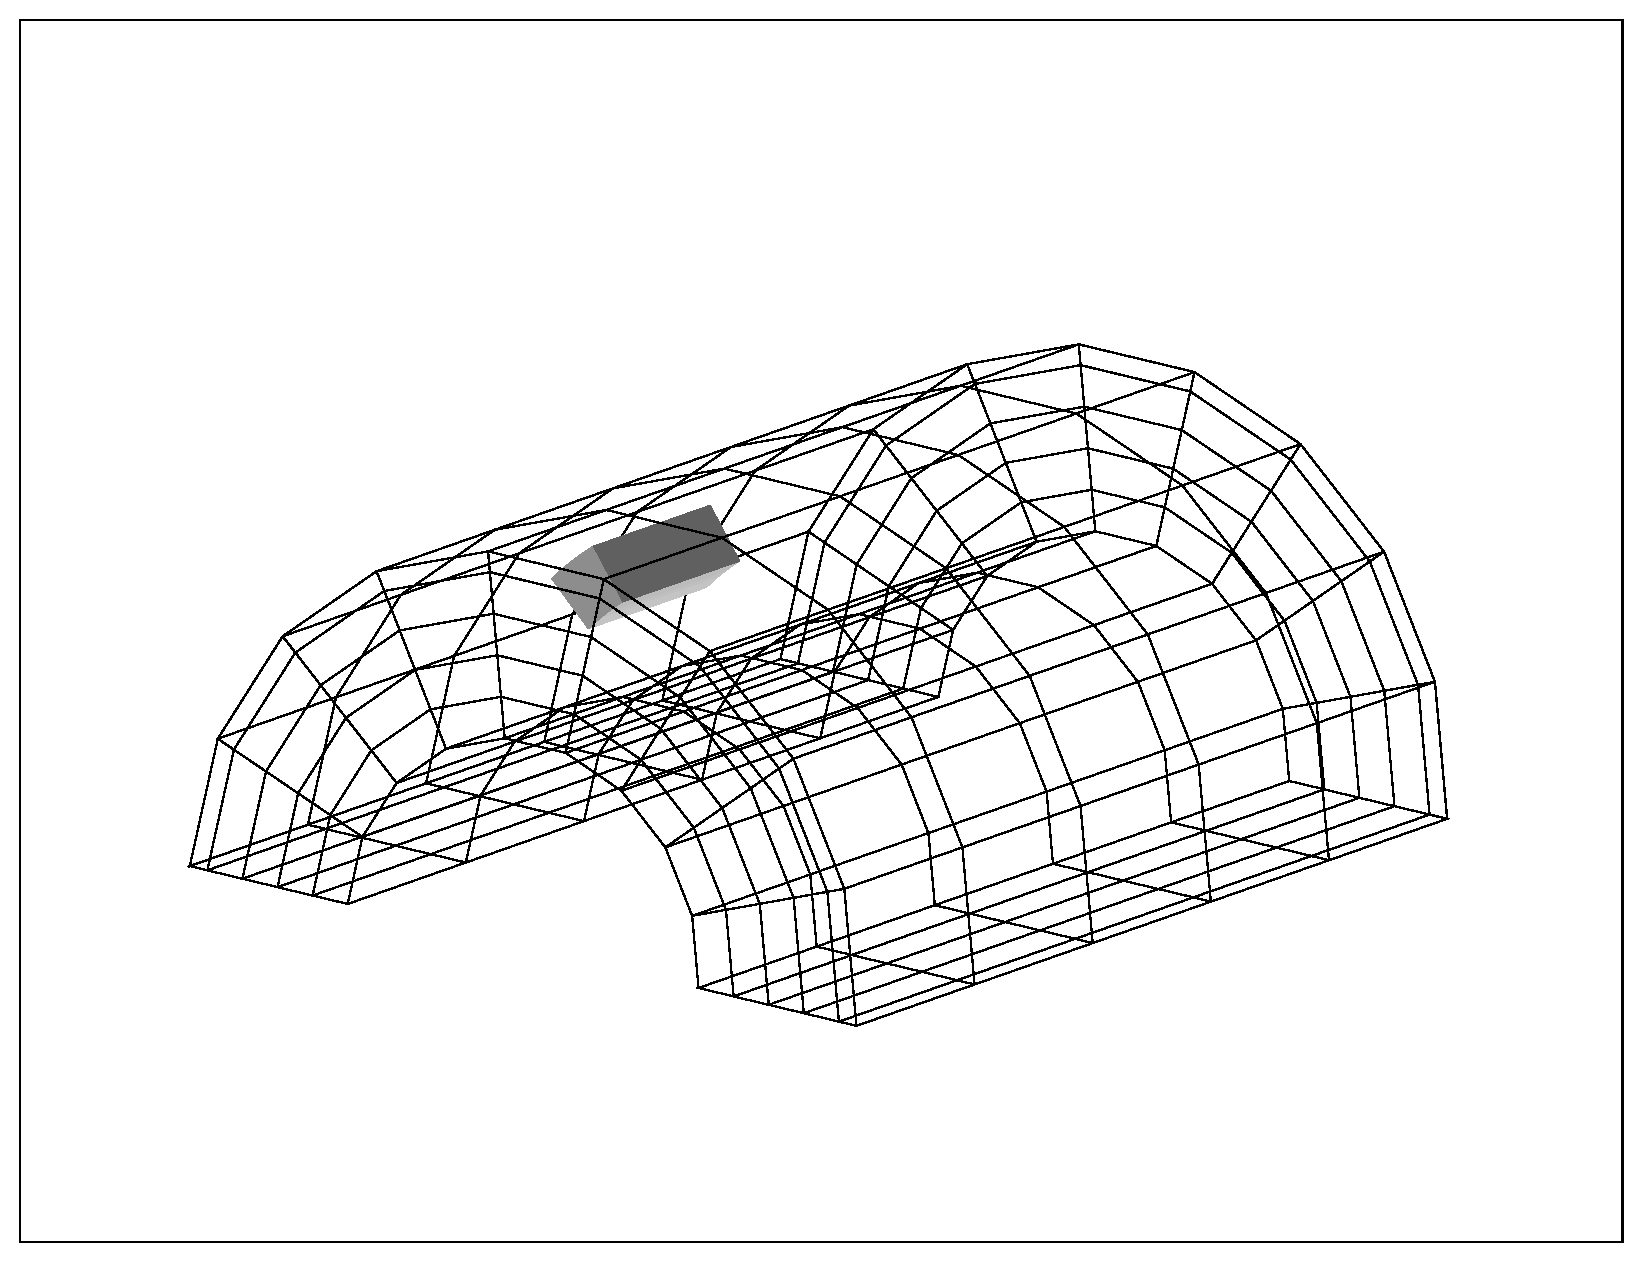
\includegraphics[width=5cm]{./cyl_grid.eps}
% One can specify [angle=x,width=y,height=z] for the graphics
\caption{Axisymmetric Grid Space}
\label{fig:grid}
\end{center}
\end{figure}

\indent In order to derive the axisymmetric Navier-Stokes equations, let us examine 
in detail an axisymmetric flow field. Fig. \ref{fig:grid} shows a half portion of a
generic axisymmetric domain, with an infantesimal region shaded within.  In order to reduce the 
computational effort required to solve a given scenario, it is convenient to express the problem 
in only two co-ordinate directions and account for the three dimensional effects through the use of
a source term.  For this approach to be correct, the flow field must be accuractly described
by a planar set of variables that can be taken to exist at any location in the circumferential
direction ($\theta$ axis).  Mathematically this condition is expressed by the following relation,

\begin{equation}
	\frac{\partial}{\partial \theta}=0 
\label{eqn:dtheta}
\end{equation}

	By further restricting the problem to a set of flow variables where the circumferential
velocity is taken as zero ($w = 0$) this eliminates the need to consider any variables in the out of plane 
dimension.  This has the effect of reducing the $\theta$ dimension to a 'void'
dimension, one that contains no flowing properties but has a physical presence in that one still
considers an infantesimal \emph{volume} when deriving the appropriate equations (also, as
will be seen in subsequent sections on turbulence, one must consider flow velocity in 
the circumferential direction for the purposes of deriving a set of axisymmetric equations,
despite the fact that the resulting equations will not contain this variable explicitly).  As well,
forces acting on the faces of the 'void' dimension must still be carefully considered as they
can in certain instances exert an influence the radial ($r$ axis) direction.  This approach is 
similar to that used when deriving a set of \emph{Quasi-2D} equations, where one makes use of 
an infantesimal	area but restricts flow variables to the first co-ordinate axis only (in essence 
creating a 'void' dimension).

	At first glance this approach may seem to contain an inconsistency in that, for example, 
in the case of supersonic flow over a cone the axisymmetric equations are able to accurately predict 
what is sometimes referred to as the three dimensional relieving effect (the reduction of the 
shock angle on a cone when compared to a wedge with an angle equal to the half angle of the cone). 
This effect is created by the fact that the flow is able to expand not only in the radial and 
axial directions, but the circumferential direction as well.  However, expansion along the 
circumferential axis by definition requires that the flow be allowed to travel in this direction, 
which as previously stated is not permitted as this dimension is declared 'void'.  

	The key to resolving this paradox lies in remembering that the Navier-Stokes equations 
deal with flows as a continuum, and as a result necessarily rely on the averaging of molecular
processes.  From a molecular viewpoint, as each particle travels along the cone it's tendency
to deviate from it's original $x$-$r$ plane is equally as likely to be left as it is to be right.  
Thus on average,for each particle traveling on a given ray that deviates to the left, 
there exists another particle traveling along this ray that deviates to the right.  This explains
why upon averaging the molecular movements, which is the basis for the Navier-Stokes equations, 
one sees no apparent movement in the circumferential direction while still being able to account
for the expansion of the flow in this direction.  

%-------------------------------------------------------------------------------------------------------------
\subsection{Species Conservation}

\begin{figure}[!h]
\begin{center}
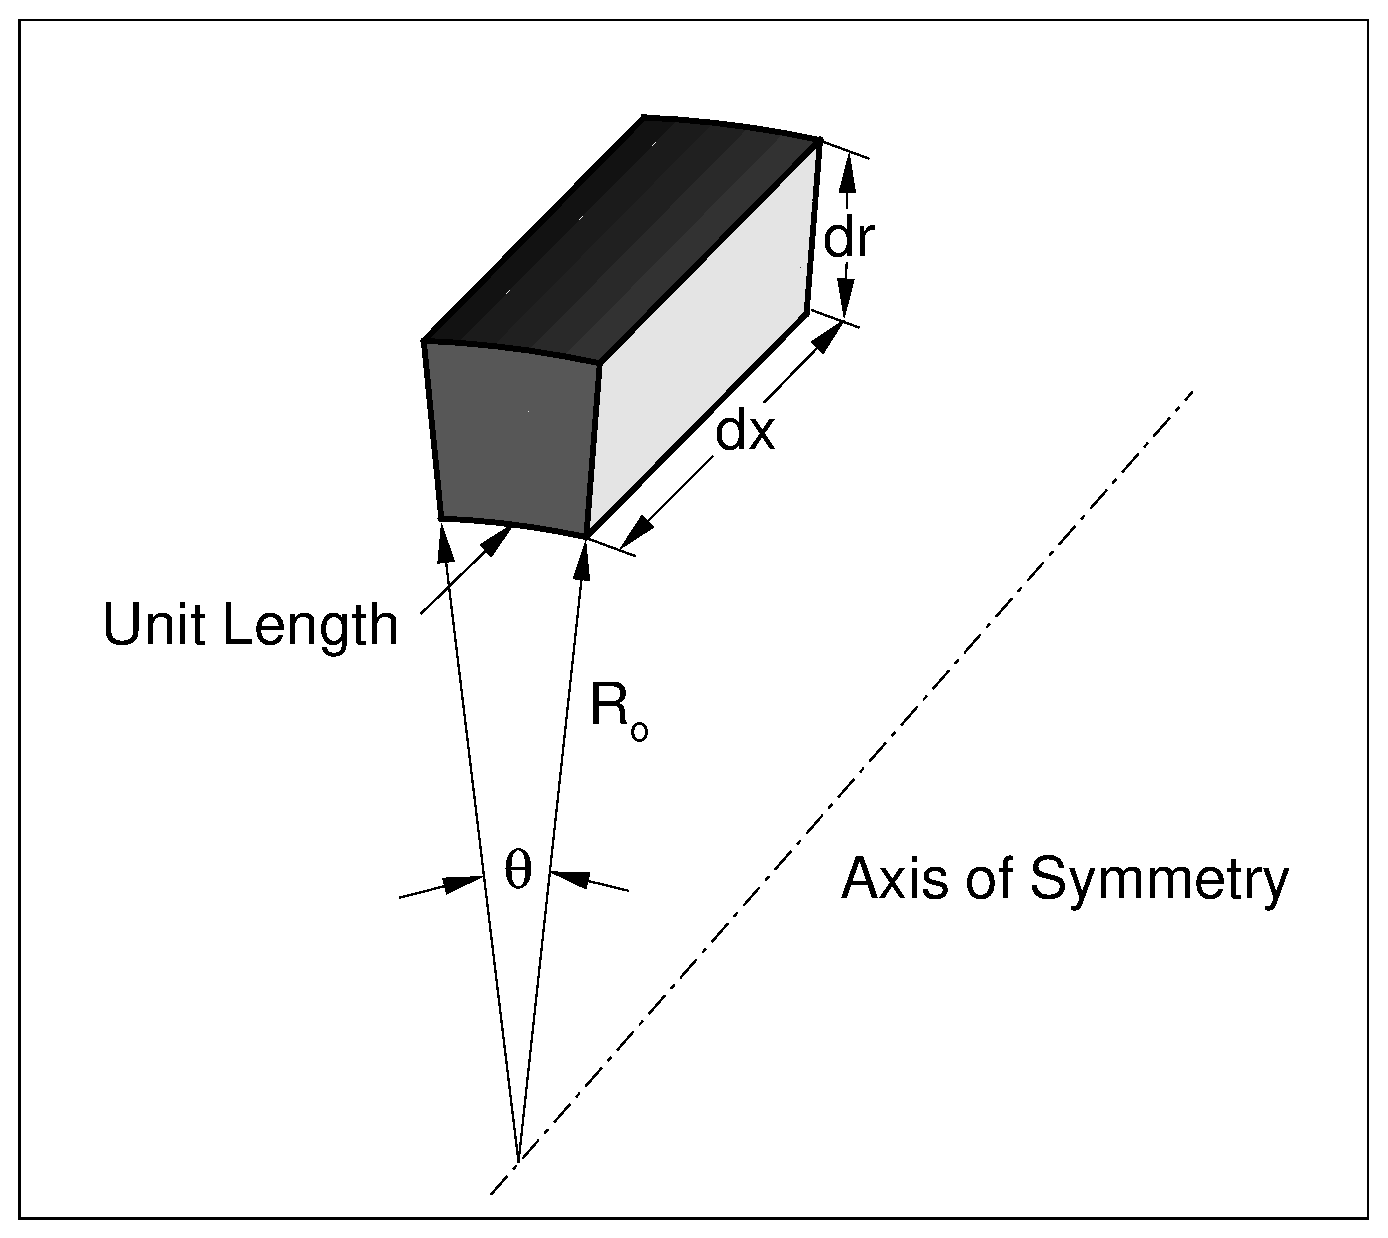
\includegraphics[width=5cm]{./infantesimal.eps}
% One can specify [angle=x,width=y,height=z] for the graphics
\caption{Infantesimal Axisymmetric Volume}
\label{fig:inftes}
\end{center}
\end{figure}

	In order to derive the conservation of mass equations for a multi-species flow, let us 
consider the infantesimal volume shown in Fig. \ref{fig:inftes}.  As can be seen, although the
equations to be derived will be for planar flow (and hence be valid in any $x$ - $r$ plane),
the fluid volume used to obtain these equations must be appropriately defined to account for the
curved nature of the $\theta$ dimension.  In this derivation, the desired
equation will be derived by considering the behaviour of the flow along each co-ordinate direction
separately and then combining the results to arrive at the final equation.



%-------------------------------------------------------------------------------------------------------------------------
\subsubsection{$x$ direction}

\begin{figure}[ht]
\includegraphics[height=5cm]{./xdir.eps}
% One can specify [angle=x,width=y,height=z] for the graphics
\caption[$r$ - $\theta$ planes]{$r$ - $\theta$ planes : All fluid properties are depicted by solid lines while 
				forces acting on the infantesimal fluid element are depicted by dashed lines (these include
				the pressure acting on the front an back $r$ - $\theta$ planes, as well as the shear
				acting on the $x$ - $r$, $x$ - $\theta$, and $r$ - $\theta$ planes)}
\label{fig:xdir}
\end{figure}

\begin{displaymath}
	\begin{array}{ccc}
		\begin{array}{c}
			\textrm{Mass flow of species \emph{k}} \\ \textrm{in through the front $r$ - $\theta$ plane} 
		\end{array} & 
	= & (\rho_k u)dr(R_o \theta) + j_{k_x} dr(R_o \theta)\\
	& \\ & \\
		\begin{array}{c}
			\textrm{Mass flow of species \emph{k}} \\ \textrm{out through the back $r$ - $\theta$ plane}
		\end{array} & 
	= & \begin{array}{c}
		(\rho_k + \frac{\partial \rho_k}{\partial x}dx)(u + \frac{\partial u}{\partial x}dx)dr(R_o \theta) \\
	+ (j_{k_x} + \frac{\partial j_{k_x}}{\partial x}dx)dr(R_o \theta)
		\end{array}
	\end{array}
\end{displaymath}

	In the above equations, $j_{k_x}$ is the diffusive flux caused by gradients existing in the concentration
of species \emph{k}, which give rise to movement of the given species in the direction opposite the gradient
(Note that $j_{k_x}$ has units of $kg/m^2 s$). All other terms are shown in Fig. \ref{fig:xdir}.
Taking the difference between these two planes (outflow - inflow) yields,

\begin{displaymath}
	\Delta \dot{m}_{k_x} = \Big\{(\rho_k u + j_{k_x} + \rho_k \frac{\partial u}{\partial x}dx + u \frac{\partial \rho_k}
	{\partial x}dx + \frac{\partial u}{\partial x} \frac{\partial \rho_k}{\partial x}dx^2 + \frac{\partial j_{k_x}}
	{\partial x}dx) - (\rho_k u + j_{k_x})\Big\} dr(R_o \theta)
\end{displaymath}

	Canceling like terms, neglecting any resulting triple products of differential quantities, and collecting terms
using the inverse of the chain rule (from the Calculus) to combine derivatives yields the following,

\begin{displaymath}
	\Delta \dot{m}_{k_x} = \Big( \frac{\partial \rho_k u}{\partial x} + \frac{\partial j_{k_x}}{\partial x}
	\Big)dxdr(R_o \theta)
\end{displaymath}
 
	It should be noted that here, and in all subsequent derivations, the area used for quantities passing through
the infantesimal volume in the $x$ direction is simply $dr(R_o \theta)$.  This assumes that the two sides of
the volume (the boundary $x$ - $r$ planes) are parallel, which is not the case as can be seen in Fig. \ref{fig:xdir}.
By making this assumption, one neglects a pie shaped area of the $r$ - $\theta$ plane, which if approximated by a 
triangle, can be calculated as,

\begin{displaymath}
	\begin{array}{ccc}
		\textrm{Area} & = & \frac{1}{2}bh \\
		\textrm{Area} & = & \frac{1}{2}\Big\{\theta(R_o + dr) - \theta(R_o)\Big\}(dr) \\
		\textrm{Area} & = & \frac{1}{2}\theta dr^2
	\end{array}
\end{displaymath}

	With the neglected area defined one can calculate the flow properties through this area as was done
previously, using $\rho_k$ as an example

\begin{displaymath}
	\begin{array}{ccc}
		\begin{array}{c}
			\textrm{Mass flow of species \emph{k}} \\ \textrm{in through the neglected area} 
		\end{array} & 
	= & (\rho_k u)(\frac{1}{2}\theta dr^2) + j_{k_x} (\frac{1}{2}\theta dr^2)\\
	& \\ & \\
		\begin{array}{c}
			\textrm{Mass flow of species \emph{k}} \\ \textrm{out through the neglected area}
		\end{array} & 
	= & \begin{array}{c}
		(\rho_k + \frac{\partial \rho_k}{\partial x}dx)(u + \frac{\partial u}{\partial x}dx)
		(\frac{1}{2}\theta dr^2) \\
	+ (j_{k_x} + \frac{\partial j_{k_x}}{\partial x}dx)(\frac{1}{2}\theta dr^2)
		\end{array}
	\end{array}
\end{displaymath}

	Again taking the diffence between the outflow minus the inflow yields,

\begin{displaymath}
	\Delta \dot{m}_{k_{\textrm{Area}}} = \Big\{(\rho_k u + j_{k_x} + \rho_k \frac{\partial u}{\partial x}dx 
					     + u \frac{\partial \rho_k}
	{\partial x}dx + \frac{\partial u}{\partial x} \frac{\partial \rho_k}{\partial x}dx^2 + \frac{\partial j_{k_x}}
	{\partial x}dx) - (\rho_k u + j_{k_x})\Big\}(\frac{1}{2}\theta dr^2)
\end{displaymath}

	Thus as shown above, after neglecting triple products and higher of differentials, the contribution of this area 
reduces to nothing.  Therefore, it is considered justified to calculate area as done previously given the fact that these 
higher order products of differentials are neglected throughout the derivation of the complete set of Navier-Stokes 
equations.

%-------------------------------------------------------------------------------------------------------------------------
\subsubsection{$r$ direction}

\begin{figure}[ht]
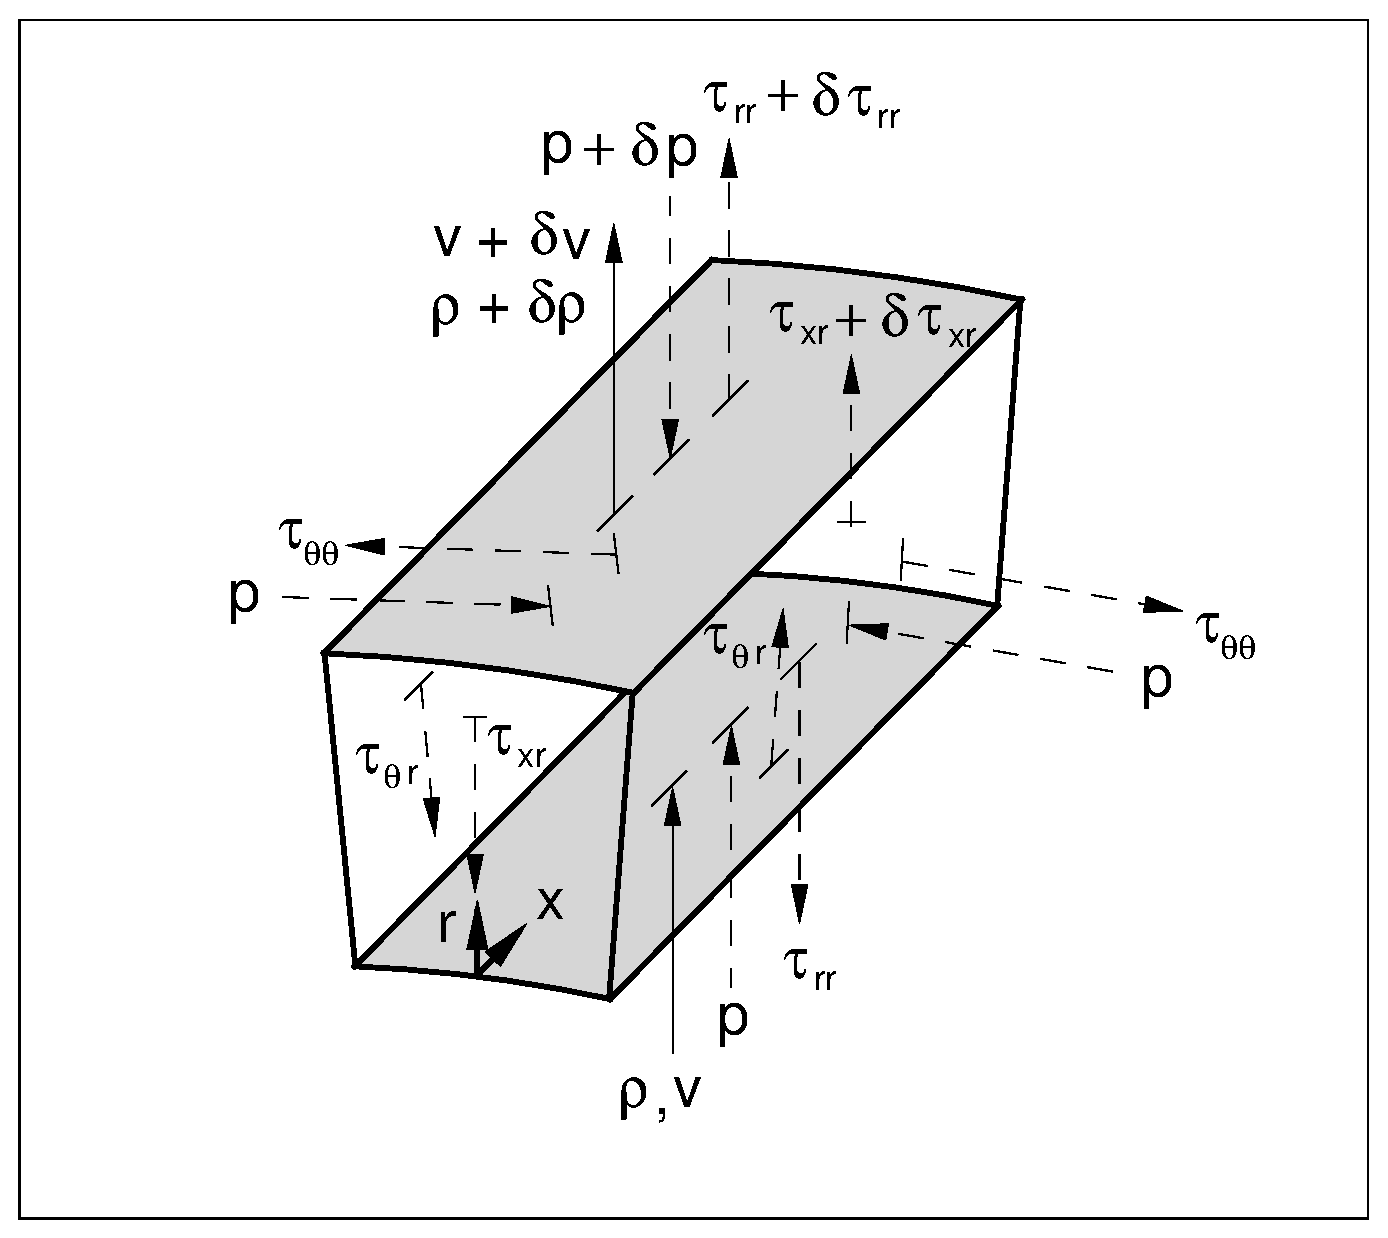
\includegraphics[height=5cm]{./rdir.eps}
% One can specify [angle=x,width=y,height=z] for the graphics
\caption[$x$ - $\theta$ planes]{$x$ - $\theta$ planes : All fluid properties are depicted by solid lines while 
				forces acting on the infantesimal fluid element are depicted by dashed lines (these include
				the pressure acting on the lower and upper $x$ - $\theta$ planes, as well as the left
				and right $x$ - $r$ planes and the shear acting on all faces of the volume)}
\label{fig:rdir}
\end{figure}

\begin{displaymath}
	\begin{array}{ccc}
		\begin{array}{c}
			\textrm{Mass flow of species \emph{k}} \\ \textrm{in through the bottom $x$ - $\theta$ plane} 
		\end{array} & 
	= & (\rho_k v)dx(R_o \theta) + j_{k_r} dx(R_o \theta)\\
	& \\ & \\
		\begin{array}{c}
			\textrm{Mass flow of species \emph{k}} \\ \textrm{out through the top $x$ - $\theta$ plane}
		\end{array} & 
	= & \begin{array}{c}
		(\rho_k + \frac{\partial \rho_k}{\partial r}dr)(v + \frac{\partial v}{\partial r}dr)dx
		(R_o + dr) \theta  \\
	+ (j_{k_r} + \frac{\partial j_{k_r}}{\partial r}dr)dx (R_o + dr) \theta
		\end{array}
	\end{array}
\end{displaymath}

	Taking the difference between the outflow and inflow in the $r$ direction yields,

\begin{displaymath}
	\begin{array}{ccc}
	\Delta \dot{m}_{k_r} & = &
		\begin{array}{c} 
	\Big\{(\rho_k v + j_{k_r} + \rho_k \frac{\partial v}{\partial r}dr + v \frac{\partial \rho_k}
	{\partial r}dr + \frac{\partial v}{\partial r} \frac{\partial \rho_k}{\partial r}dr^2 + \frac{\partial j_{k_r}}
	{\partial r}dr) -\rho_k v - j_{k_r}\Big\} dx(R_o \theta) \\
	+ (\rho_k v + j_{k_r} + \rho_k \frac{\partial v}{\partial r}dr + v \frac{\partial \rho_k}
	{\partial r}dr + \frac{\partial v}{\partial r} \frac{\partial \rho_k}{\partial r}dr^2 + \frac{\partial j_{k_r}}
	{\partial r}dr) dx dr \theta
		\end{array}
	\end{array}
\end{displaymath}

	Again combining differentials using the inverse of the chain rule and neglecting triple products (and higher)
of differentials, the above equation reduces to the following,

\begin{displaymath}
	\Delta \dot{m}_{k_r} = \Big( \frac{\partial \rho_k v}{\partial r} + \frac{\partial j_{k_r}}{\partial r}
	\Big)dxdr(R_o \theta) + (\rho_k v + j_{k_r})dxdr\theta
\end{displaymath}

	Applying the principle of mass conservation, any unsteady change in $\rho_k$ plus the sum of the mass fluxes in 
each of the co-ordinate directions must sum to zero,

\begin{displaymath}
	\begin{array}{ccc}
	\frac{\partial \rho_k}{\partial t}dxdr(R_o \theta) + \Delta \dot{m}_{k_x} + \Delta \dot{m}_{k_r} & = & 0 \\
	\Big\{(\frac{\partial \rho_k}{\partial t} + \frac{\partial \rho_k u}{\partial x} + \frac{\partial j_{k_x}}{\partial x}
	+  \frac{\partial \rho_k v}{\partial r} + \frac{\partial j_{k_r}}{\partial r})(R_o \theta) + 
	(\rho_k v + j_{k_r})\theta \Big\}dxdr & = & 0
	\end{array}
\end{displaymath}

	Without loss in generality, one can let $R_o \theta$ = 1 as shown in Fig. \ref{fig:inftes} and if one rewrites $R_o$ 
as $r$ then $\theta$ can be expressed as,	

\begin{equation}
	\theta = \frac {1}{r}
\label{eqn:theta}
\end{equation}

	which then allows the axisymmetric species conservation equation to be written as,

\begin{equation}
	\frac{\partial \rho_k}{\partial t} + \frac{\partial \rho_k u}{\partial x} + \frac{\partial \rho_k v}{\partial r}
	+ \frac {1}{r}(\rho_k v) = -\frac{\partial j_{k_x}}{\partial x} - \frac{\partial j_{k_r}}{\partial r} - \frac {1}{r}
	(j_{k_r})
\label{eqn:species}
\end{equation}

	For multi-species flow, the total density can be expressed as the sum of the individual species densities

\begin{equation}
	\sum_{i} \rho_k
\end{equation}

	while the concentration of species \emph{k}, $c_k$, can be written as 

\begin{equation}
	\rho_k = c_k \rho
\label{eqn:conc}
\end{equation}

	To express the diffusive flux in term of species concentrations one can use Fick's Law,

\begin{equation}
	j_{k_x} = - \rho D_{kl} \frac{\partial c_k}{\partial x}
\label{eqn:fick}
\end{equation}

	where $D_{kl}$ is the binary diffusion coefficient representing the degree to which gas $k$ will tend to 
diffuse into gas $l$ and the negative sign reflects the fact that the gas diffuses in the direction opposite the
concentration gradient (also note $j_{k_r}$ is similarly defined).  If we define another co-efficient $\nu_i$ as,

\begin{equation}
	\nu_k = \rho D_{kl}
\label{eqn:nuk}
\end{equation}

	then by substituting Eqs. \ref{eqn:fick} and \ref{eqn:nuk} into Eq. \ref{eqn:species} one obtains 

\begin{equation}
	\frac{\partial}{\partial t}(\rho_k) + \frac{\partial}{\partial x}(\rho_k u) + \frac{\partial}{\partial r}(\rho_k v)
	+ \frac {1}{r}(\rho_k v) = \frac{\partial}{\partial x}(\nu_k \frac{\partial c_k}{\partial x}) + \frac{\partial}
	{\partial r}(\nu_k \frac{\partial c_k}{\partial r}) + \frac {1}{r}(\nu_k \frac{\partial c_k}{\partial r})
\label{eqn:speciesfinal}
\end{equation}

	To obtain the global continuity equation, simply sum Eq.\ref{eqn:speciesfinal} over all the species present.
Since the sum of the species concentrations is unity ($\sum c_k = 1$), the sum of $\rho_k$ simplifies to $\rho$ 
(see Eq.\ref{eqn:conc} while any derivatives involving species concentrations reduce to zero yielding,

\begin{equation}
	\frac{\partial}{\partial t}(\rho) + \frac{\partial}{\partial x}(\rho u) + \frac{\partial}{\partial r}(\rho v)
	+ \frac{1}{r}(\rho v) = 0
\label{eqn:globalcont}
\end{equation}
	
%---------------------------------------------------------------------------------------------------------------------------
\subsection{Momentum Along the $x$ Co-Ordinate Direction}

	In order to derive the momentum equations in both the $x$ and $r$ directions, we will again make use of Figs.
\ref{fig:xdir} and \ref{fig:rdir}.  Since the desired equations are based on Newton's second law, ($F=ma$), the forces
acting on the surface of the infantesimal volume must be properly considered as it is these forces which balance the 
net change in momentum of the volume.  It should be noted at this point that given the axisymmetric assumption 
(Eq.\ref{eqn:dtheta}) no quantites passing through the $x$ - $r$ planes need be considered as there will be no net 
change in these quantites (i.e. the net change in $x$ momentum passing through these planes will be zero).  This 
also hold true for the $r$ co-ordinate direction.    

\begin{displaymath}
	\begin{array}{ccc}
		\textrm{$x$ Momentum in through the front $r$ - $\theta$ plane} &
		= & (\rho u)(u)dr(R_o \theta)\\
 		& \\ & \\
		\textrm{$x$ Momentum out through the back $r$ - $\theta$ plane} &
		= & (\rho u + \frac{\partial \rho u}{\partial x}dx)(u + \frac{\partial u}{\partial x}dx)dr(R_o \theta) 
	\end{array}
\end{displaymath}

	Taking the difference between the outflow and inflow $r$ - $\theta$ planes yields,

\begin{displaymath}
	\begin{array}{c}
	\Delta x_{momentum_{r \theta}}=(\rho u^2 + \rho u \frac{\partial u}{\partial x}dx + 
	u \frac{\partial \rho u}{\partial x}dx +
	\frac{\partial\rho u}{\partial x} \frac{\partial u}{\partial x}dx^2 - \rho u^2)dr(R_o \theta) \\ \\
	\Delta x_{momentum_{r \theta}}=(\frac{\partial \rho u^2}{\partial x})dxdr(R_o \theta)
	\end{array}
\end{displaymath}

	after combining derivatives and neglecting triple products of differentials.

\begin{displaymath}
	\begin{array}{ccc}
		\textrm{$x$ Momentum in through the bottom $x$ - $\theta$ plane} &
		= & (\rho v)(u)dx(R_o \theta)\\
 		& \\ & \\
		\textrm{$x$ Momentum out through the top $x$ - $\theta$ plane} &
		= & (\rho v + \frac{\partial \rho v}{\partial r}dr)(u + \frac{\partial u}{\partial r}dr)dx
		(R_o + dr) \theta 
	\end{array}
\end{displaymath}

	Taking the difference between the outflow and inflow $x$ - $\theta$ planes yields,

\begin{displaymath}
	\begin{array}{c}
	\Delta x_{momentum_{x \theta}}=
		\begin{array}{c}
	(\rho uv + \rho v \frac{\partial u}{\partial r}dr + 
	u \frac{\partial \rho v}{\partial r}dr + \frac{\partial u}{\partial r} \frac{\partial \rho v}{\partial r}dr^2 -
	\rho uv)dx(R_o \theta) \\
	 + (\rho uv + \rho v \frac{\partial u}{\partial r}dr + u \frac{\partial \rho v}{\partial r}dr + 
	\frac{\partial u}{\partial r} \frac{\partial \rho v}{\partial r}dr^2)dxdr \theta
		\end{array} \\ \\
	\Delta x_{momentum_{x \theta}}= (\frac{\partial \rho uv}{\partial r})dxdr (R_o \theta) + (\rho uv)dxdr \theta
	\end{array}
\end{displaymath}

	after again simplifying and neglecting triple products and higher of differential quantities.  Allowing for an
unsteady change in the $x$ direction momentum and applying Newton's second law yields,

\begin{displaymath}
	\frac{\partial \rho u}{\partial t}dxdr(R_o \theta) + \Delta x_{momentum_{r \theta}} + \Delta x_{momentum_{x \theta}} = 
	\sum \textrm{Forces}_x
\end{displaymath}

	which after making the appropriate substitutions yields

\begin{displaymath}
	\Big\{(\frac{\partial \rho u}{\partial t} + \frac{\partial \rho u^2}{\partial x} +
	\frac{\partial \rho uv}{\partial r})(R_o \theta) + (\rho u v) \theta\Big\}dxdr = \sum \textrm{Forces}_x
\end{displaymath}

	However, $\theta$ can be eliminated through the use of Eq. \ref{eqn:theta} to obtain

\begin{equation}
	\Big\{\frac{\partial \rho u}{\partial t} + \frac{\partial \rho u^2}{\partial x} +
	\frac{\partial \rho uv}{\partial r} + \frac{1}{r}(\rho u v)\Big\}dxdr = \sum \textrm{Forces}_x
\label{eqn:xmomchg}
\end{equation}

	To complete the right side of Eq.\ref{eqn:xmomchg}, one needs to consider the forces acting in the $x$ direction,
shown in Fig. \ref{fig:xdir} as dashed lines.
The forces that need to be considered are the pressure acting on the $r$ - $\theta$ planes 
(which always acts towards the interior of the volume), the tangential shear acting on the $x$ - $r$ and $x$ - $\theta$ 
planes ($\tau_{\theta x}$ and $\tau_{rx}$ respectively),
and the normal shear acting as well on the $r$ - $\theta$ planes (which always acts away from the interior
of the volume).  Also note that if turbulence is being considered then the pressure is the sum of the thermodynamic
pressure (as defined by some appropriate equation of state) and the turbulent pressure (which depends on the kinetic
energy of turbulence, $\rho k$)

\begin{displaymath}
	p = p_{thermodynamic} + \frac{2}{3}\rho k
\end{displaymath}

\begin{displaymath}
	\begin{array}{ccc}
		\begin{array}{c}
		\textrm{Force exerted on the front $r$ - $\theta$ plane} \\
		\textrm{by the pressure on its surface}
		\end{array} & = &
		p dr (R_o \theta) \\
	& \\ & \\
		\begin{array}{c}
		\textrm{Force exerted on the back $r$ - $\theta$ plane}\\
		\textrm{by the pressure on its surface}
		\end{array} & = &
		-(p + \frac{\partial p}{\partial x}dx) dr (R_o \theta) 
	\end{array} 
\end{displaymath}
\\
\begin{displaymath}
	\begin{array}{ccc}
		\begin{array}{c}
		\textrm{Force exerted on the front $r$- $\theta$ plane} \\
		\textrm{by the shear on its surface}
		\end{array} & = &
		- \tau_{xx}dr (R_o \theta) \\
   	& \\ & \\
		\begin{array}{c}
		\textrm{Force exerted on the back $r$ - $\theta$ plane}\\
		\textrm{by the shear on its surface}
		\end{array} & = &
		(\tau_{xx} + \frac{\partial \tau_{xx}}{\partial x}dx) dr (R_o \theta) 
	\end{array}
\end{displaymath}
\\
\begin{displaymath}
	\begin{array}{ccc}
		\begin{array}{c}
		\textrm{Force exerted on the bottom $x$ - $\theta$ plane}\\
		\textrm{by the shear on its surface}
		\end{array} & = &
		- \tau_{rx}dx(R_o \theta) \\
	& \\ & \\
		\begin{array}{c}
		\textrm{Force exerted on the top $x$ - $\theta$ plane} \\
		\textrm{by the shear on its surface}
		\end{array} & = &
		(\tau_{rx} + \frac{\partial \tau_{rx}}{\partial r}dr)dx(R_o + dr)\theta
	\end{array} 
\end{displaymath}

	Note that since the remaining shear acting in the $x$ direction, $\tau_{\theta x}$, is independent of the $x$ - $r$
plane upon which it acts due to the condition expressed in Eq. \ref{eqn:dtheta}, by inspection one can see that the forces
created by these shears will exactly cancel out in the $x$ direction.  However, summing the remaining terms yields,

\begin{displaymath}
	\begin{array}{ccc}
	\sum \textrm{Forces}_x & = &
		\begin{array}{c}
			(pdr - pdr - \frac{\partial p}{\partial x}dxdr - \tau_{xx}dr + \tau_{xx}dr + \frac{\partial \tau_{xx}}
			{\partial x}dxdr \\
			- \tau_{rx}dx + \tau_{rx}dx + \frac{\partial \tau_{rx}}{\partial r}dxdr)(R_o \theta)
			+ (\tau_{rx} + \frac{\partial \tau_{rx}}{\partial r}dr)dxdr \theta
		\end{array}
	\end{array}
\end{displaymath}

	which after canceling like terms, inserting Eq. \ref{eqn:theta} to replace $\theta$, and neglecting 
triple products of differentials reduces to

\begin{equation}
	\begin{array}{ccc}
	\sum \textrm{Forces}_x & = &
		(- \frac{\partial p}{\partial x} + \frac{\partial \tau_{xx}}{\partial x}
		+ \frac{\partial \tau_{rx}}{\partial r} + \frac{1}{r}\tau_{rx})dxdr
	\end{array}
\label{eqn:xforces}
\end{equation}

	Combining Eqs. \ref{eqn:xmomchg} and \ref{eqn:xforces} one obtains

\begin{equation}
\Big\{\frac{\partial}{\partial t}(\rho u) + \frac{\partial}{\partial x}(\rho u^2) +
\frac{\partial}{\partial r}(\rho uv) + \frac{1}{r}(\rho u v)\Big\}dxdr = \Big\{ - \frac{\partial}{\partial x}(p) 
+ \frac{\partial}{\partial x}(\tau_{xx}) + \frac{\partial}{\partial r}(\tau_{rx}) + \frac{1}{r}(\tau_{rx})\Big\}dxdr
\label{eqn:xmomshear}
\end{equation}

\subsubsection{Definition of the Viscous Stresses}

	From the mechanics of Newtonian fluids the stresses can be defined using derivatives of the 
co-ordinate velocities as follows

\begin{equation}
	\tau_{rx} = \tau_{xr} = \mu(\frac{\partial v}{\partial x} + \frac{\partial u}{\partial r})
\label{eqn:taurx}
\end{equation}

\begin{equation}
	\tau_{xx} = \lambda(\nabla \cdot \vec{V}) + 2 \mu \frac{\partial u}{\partial x}
\label{eqn:tauxxlambda}
\end{equation}

\begin{equation}
	\tau_{rr} = \lambda(\nabla \cdot \vec{V}) + 2 \mu \frac{\partial v}{\partial r}
\label{eqn:taurrlambda}
\end{equation}

\begin{displaymath}
	\tau_{\theta \theta} = \lambda(\nabla \cdot \vec{V}) + 2 \mu (\frac{1}{r} \frac{\partial w}{\partial \theta} + \frac{v}{r})
\end{displaymath}

	which for the axisymmetric case (Eq. \ref{eqn:dtheta}) reduces to 

\begin{equation}
	\tau_{\theta \theta} = \lambda(\nabla \cdot \vec{V}) + 2 \mu \frac{v}{r}	
\label{eqn:tauthetathetalambda}
\end{equation}
	
	The quantity $\vec{V}$ is the vector sum of the co-ordinate velocties and $\mu$ is the coefficient of 
viscosity of the fluid under consideration.  In order to evaluate the dot product of the del operator ($\nabla$) on 
the velocity vector ($\vec{V}$) one must remember to use the cylindrical co-ordinate system,

\begin{displaymath}
	\nabla \cdot \vec{V} = \frac{\partial u}{\partial x} + \frac{1}{r} \frac{\partial rv}{\partial r} + \frac{1}{r}
	\frac{\partial w}{\partial \theta}
\end{displaymath}

	which after applying the axisymmetric condition (Eq. \ref{eqn:dtheta}) and the chain rule from the Calculus
can be reduced to

\begin{equation}
	\nabla \cdot \vec{V} = \frac{\partial u}{\partial x} +  \frac{\partial v}{\partial r} + \frac{v}{r}
\label{eqn:delv}
\end{equation}

	With the help of Stokes' hypothesis which states

\begin{equation}
	\lambda = -\frac{2}{3} \mu
\label{eqn:stokes}
\end{equation}

	one can rewrite the stress quantities in terms of velocity component derivatives by substituting Eqs. \ref{eqn:delv} and
\ref{eqn:stokes} into Eqs. \ref{eqn:tauxxlambda} - \ref{eqn:tauthetathetalambda},

\begin{displaymath}
	\tau_{xx} = - \frac{2}{3} \mu (\frac{\partial u}{\partial x} + \frac{\partial v}{\partial r} + \frac{v}{r}) 
	+ \frac{6}{3} \mu \frac{\partial u}{\partial x}
\end{displaymath}

\begin{displaymath}
	\tau_{xx} = \mu ( \frac{4}{3} \frac{\partial u}{\partial x} - \frac{2}{3} \frac{\partial v}{\partial r})  
	- \mu \frac{2}{3} \frac{v}{r} 
\end{displaymath}

\begin{displaymath}
	\tau_{rr} = - \frac{2}{3} \mu (\frac{\partial u}{\partial x} + \frac{\partial v}{\partial r} + \frac{v}{r}) 
	+ \frac{6}{3} \mu \frac{\partial v}{\partial x}
\end{displaymath}

\begin{displaymath}
	\tau_{rr} = \mu ( - \frac{2}{3} \frac{\partial u}{\partial x} + \frac{4}{3} \frac{\partial v}{\partial r})  
	- \mu \frac{2}{3} \frac{v}{r} 
\end{displaymath}

\begin{displaymath}
	\tau_{\theta \theta} = - \frac{2}{3} \mu (\frac{\partial u}{\partial x} + \frac{\partial v}{\partial r} 
	+ \frac{v}{r}) + \frac{6}{3}\mu \frac{v}{r}
\end{displaymath}

\begin{equation}
	\tau_{\theta \theta} = \mu \Big\{- \frac{2}{3} (\frac{\partial u}{\partial x} + \frac{\partial v}{\partial r})  
	+ \frac{4}{3} \frac{v}{r} \Big\} 
\label{eqn:tauthetatheta}
\end{equation}

	If we further define $\hat{\tau}_{xx}$ and $\hat{\tau}_{rr}$ to be 

\begin{equation}
	\hat{\tau}_{xx} =  \mu ( \frac{4}{3} \frac{\partial u}{\partial x} - \frac{2}{3} \frac{\partial v}{\partial r})  
\label{eqn:tauxxhat}
\end{equation}

\begin{equation}
	\hat{\tau}_{rr} =  \mu ( - \frac{2}{3} \frac{\partial u}{\partial x} + \frac{4}{3} \frac{\partial v}{\partial r})  
\label{eqn:taurrhat}
\end{equation}

	then

\begin{equation}
	\tau_{xx} = \hat{\tau}_{xx} - \mu \frac{2}{3} \frac {v}{r}
\label{eqn:tauxx}
\end{equation}

\begin{equation}
	\tau_{rr} = \hat{\tau}_{rr} - \mu \frac{2}{3} \frac{v}{r}
\label{eqn:taurr}
\end{equation}

	This step of defining $\hat{\tau}$ is done so that all differences between the axisymmetric and more
conventional 2D equations can be kept to a single source term, since $\hat{\tau}$ now matches exactly the stresses
found from a 2D Cartesian derivation.
	
	Finally, by using the results of Eq. \ref{eqn:tauxx} in Eq. \ref{eqn:xmomshear} and 
rearranging leaving only viscosity related terms on the right side of the equation, one obtains the 
desired form of the $x$ direction momentum equation

\begin{equation}
\frac{\partial}{\partial t}(\rho u) + \frac{\partial}{\partial x}(\rho u^2 + p) +
\frac{\partial}{\partial r}(\rho uv) + \frac{1}{r}(\rho u v) = 
\frac{\partial}{\partial x}(\hat{\tau}_{xx}) + \frac{\partial}{\partial r}(\tau_{rx}) + 
\frac{1}{r}(\tau_{rx}) - \frac{2}{3} \frac{\partial}{\partial x}(\mu \frac{v}{r})
\label{eqn:xmom}
\end{equation}

	with the stresses defined by their respective Eqs.\ref{eqn:taurx} and \ref{eqn:tauxxhat}.

%---------------------------------------------------------------------------------------------------------------------------
\subsection{Momentum Along the $r$ Co-Ordinate Direction}

	To obtain this equation, one needs to consider the quantities shown in Fig. \ref{fig:rdir}.  The derivation of 
this equation is similar to that of the $x$ direction but for a few extra terms acting in the $\theta$ direction that need 
be considered due to their influence in the $r$ direction.

\begin{displaymath}
	\begin{array}{ccc}
		\textrm{$r$ Momentum in through the bottom $x$ - $\theta$ plane} &
		= & (\rho v)(v)dx(R_o \theta)\\
 		& \\ & \\
		\textrm{$r$ Momentum out through the top $x$ - $\theta$ plane} &
		= & (\rho v + \frac{\partial \rho v}{\partial r}dr)(v + \frac{\partial v}{\partial r}dr)dx
		(R_o + dr) \theta 
	\end{array}
\end{displaymath}


	Taking the difference between the outflow and inflow $x$ - $\theta$ planes yields,

\begin{displaymath}
	\begin{array}{c}
	\Delta r_{momentum_{x \theta}}=
		\begin{array}{c}
	(\rho v^2 + \rho v \frac{\partial v}{\partial r}dr + 
	v \frac{\partial \rho v}{\partial r}dr + \frac{\partial v}{\partial r} \frac{\partial \rho v}{\partial r}dr^2 -
	\rho v^2)dx(R_o \theta) \\
	 + (\rho v^2 + \rho v \frac{\partial v}{\partial r}dr + v \frac{\partial \rho v}{\partial r}dr + 
	\frac{\partial v}{\partial r} \frac{\partial \rho v}{\partial r}dr^2)dxdr \theta
		\end{array} \\ \\
	\Delta r_{momentum_{x \theta}}= (\frac{\partial \rho v^2}{\partial r})dxdr (R_o \theta) + (\rho v^2)dxdr \theta
	\end{array}
\end{displaymath}

\begin{displaymath}
	\begin{array}{ccc}
		\textrm{$r$ Momentum in through the front $r$ - $\theta$ plane} &
		= & (\rho v)(u)dr(R_o \theta)\\
 		& \\ & \\
		\textrm{$r$ Momentum out through the back $r$ - $\theta$ plane} &
		= & (\rho v + \frac{\partial \rho v}{\partial x}dx)(u + \frac{\partial u}{\partial x}dx)dr(R_o \theta) 
	\end{array}
\end{displaymath}

	Taking the difference between the outflow and inflow $r$ - $\theta$ planes yields,

\begin{displaymath}
	\begin{array}{c}
	\Delta r_{momentum_{r \theta}}=(\rho uv + \rho v \frac{\partial u}{\partial x}dx + 
	u \frac{\partial \rho v}{\partial x}dx +
	 \frac{\partial u}{\partial x} \frac{\partial\rho v}{\partial x}dx^2 - \rho uv)dr(R_o \theta) \\ \\
	\Delta r_{momentum_{r \theta}}=(\frac{\partial \rho uv}{\partial x})dxdr(R_o \theta)
	\end{array}
\end{displaymath}

	As before, allowing for an unsteady change in the $r$ direction momentum and applying Newton's second law

\begin{displaymath}
	\frac{\partial \rho v}{\partial t}dxdr(R_o \theta) + \Delta r_{momentum_{r \theta}} + \Delta r_{momentum_{x \theta}} = 
	\sum \textrm{Forces}_r
\end{displaymath}

	which after making the appropriate substitutions yields

\begin{displaymath}
	\Big\{(\frac{\partial \rho v}{\partial t} + \frac{\partial \rho uv}{\partial x} +
	\frac{\partial \rho v^2}{\partial r})(R_o \theta) + (\rho v^2 \theta)\Big\}dxdr = \sum \textrm{Forces}_r
\end{displaymath}

	However, $\theta$ can be eliminated through the use of Eq. \ref{eqn:theta} to obtain

\begin{equation}
	\Big\{\frac{\partial \rho v}{\partial t} + \frac{\partial \rho uv}{\partial x} +
	\frac{\partial \rho v^2}{\partial r} + \frac{1}{r}(\rho v^2)\Big\}dxdr = \sum \textrm{Forces}_r
\label{eqn:rmomchg}
\end{equation}

	Again examining each of the forces contributing to an overall force in the $r$ direction individually one 
can complete the right hand side of Eq.\ref{eqn:rmomchg}.

\begin{displaymath}
	\begin{array}{ccc}
		\begin{array}{c}
		\textrm{Force exerted on the bottom $x$ - $\theta$ plane} \\
		\textrm{by the pressure on its surface}
		\end{array} & = &
		p dx (R_o \theta) \\
	& \\ & \\
		\begin{array}{c}
		\textrm{Force exerted on the top $x$ - $\theta$ plane}\\
		\textrm{by the pressure on its surface}
		\end{array} & = &
		-(p + \frac{\partial p}{\partial r}dr) dx (R_o + dr) \theta
	\end{array} 
\end{displaymath}
\\
\begin{displaymath}
	\begin{array}{ccc}
		\begin{array}{c}
		\textrm{Force exerted on the bottom $x$- $\theta$ plane} \\
		\textrm{by the shear on its surface}
		\end{array} & = &
		- \tau_{rr}dx (R_o \theta) \\
   	& \\ & \\
		\begin{array}{c}
		\textrm{Force exerted on the top $x$ - $\theta$ plane}\\
		\textrm{by the shear on its surface}
		\end{array} & = &
		(\tau_{rr} + \frac{\partial \tau_{rr}}{\partial r}dr) dx (R_o + dr) \theta
	\end{array}
\end{displaymath}

\begin{displaymath}
	\begin{array}{ccc}
		\begin{array}{c}
		\textrm{Force exerted on the front $r$- $\theta$ plane} \\
		\textrm{by the shear on its surface}
		\end{array} & = &
		- \tau_{xr}dr (R_o \theta) \\
   	& \\ & \\
		\begin{array}{c}
		\textrm{Force exerted on the back $r$ - $\theta$ plane}\\
		\textrm{by the shear on its surface}
		\end{array} & = &
		(\tau_{xr} + \frac{\partial \tau_{xr}}{\partial x}dx) dr (R_o \theta) 
	\end{array}
\end{displaymath}

	Now, by symmetry, it can be see that since $\tau_{\theta r}$ acts in opposite directions and on opposite
faces of the fluid element, it's net effect in the $r$ direction will be zero due to the axisymmetric condtion
expressed by Eq.\ref{eqn:dtheta}.  This can be illustrated by the following.  If one places the $x$ - $r$ plane
at the centre of the infantesimal volume, then the distance to each boundary $x$ - $r$ plane (the left and right sides
of the volume) is $\frac{\theta}{2}$.  The component of $\tau_{\theta r}$ acting on each of these faces in the $r$ 
direction is $\tau_{\theta r}\cos{\frac{\theta}{2}}$.  Therefore, given that the direction each of these components 
acts is opposed, their overall contribution to the right hand side of Eq.\ref{eqn:rmomchg} is zero.  However, the same 
cannot be said for $\tau_{\theta \theta}$, and indeed $p$, which also 
acts on these surfaces.  In these cases, there is a net effect which must be accounted for as follows.

\begin{displaymath}
	\begin{array}{ccc}
		\begin{array}{c}
		\textrm{Force exerted on the left $x$- $r$ plane} \\
		\textrm{in the $r$ direction} \\
		\textrm{by the shear on its surface}
		\end{array} & = &
		- \tau_{\theta \theta}\sin{\frac{\theta}{2}}dxdr \\
   	& \\ & \\
		\begin{array}{c}
		\textrm{Force exerted on the right $x$ - $r$ plane}\\
		\textrm{in the $r$ direction} \\
		\textrm{by the shear on its surface}
		\end{array} & = &
		- \tau_{\theta \theta}\sin{\frac{\theta}{2}}dxdr
	\end{array}
\end{displaymath}  

\begin{displaymath}
	\begin{array}{ccc}
		\begin{array}{c}
		\textrm{Force exerted on the left $x$- $r$ plane} \\
		\textrm{in the $r$ direction} \\
		\textrm{by the pressure on its surface}
		\end{array} & = &
		p \sin{\frac{\theta}{2}}dxdr \\
   	& \\ & \\
		\begin{array}{c}
		\textrm{Force exerted on the right $x$ - $r$ plane}\\
		\textrm{in the $r$ direction} \\
		\textrm{by the pressre on its surface}
		\end{array} & = &
		p \sin{\frac{\theta}{2}}dxdr
	\end{array}
\end{displaymath}  

	but for small angles (as is the case for an infantesimal volume),

\begin{equation}
	\sin{\theta} = \theta
\label{eqn:smallangle}
\end{equation}

	therefore,

\begin{displaymath}
	\begin{array}{ccc}
		\begin{array}{c}
		\textrm{Force exerted on the left $x$- $r$ plane} \\
		\textrm{in the $r$ direction} \\
		\textrm{by the shear on its surface}
		\end{array} & = &
		- \frac{1}{2}\tau_{\theta \theta}\theta dxdr \\
   	& \\ & \\
		\begin{array}{c}
		\textrm{Force exerted on the right $x$ - $r$ plane}\\
		\textrm{in the $r$ direction} \\
		\textrm{by the shear on its surface}
		\end{array} & = &
		- \frac{1}{2} \tau_{\theta \theta}\theta dxdr
	\end{array}
\end{displaymath}

\begin{displaymath}
	\begin{array}{ccc}
		\begin{array}{c}
		\textrm{Force exerted on the left $x$- $r$ plane} \\
		\textrm{in the $r$ direction} \\
		\textrm{by the pressure on its surface}
		\end{array} & = &
		\frac{1}{2}p \theta dxdr \\
   	& \\ & \\
		\begin{array}{c}
		\textrm{Force exerted on the right $x$ - $r$ plane}\\
		\textrm{in the $r$ direction} \\
		\textrm{by the pressure on its surface}
		\end{array} & = &
		\frac{1}{2}p \theta dxdr
	\end{array}
\end{displaymath}

	Summing all the forces considered, the total force in the $r$ - direction yields,

\begin{displaymath}
	\begin{array}{ccc}
	\sum \textrm{Forces}_r & = &
		\begin{array}{c}
			(pdx - pdx  - \frac{\partial p}{\partial r}dxdr - \tau_{rr}dx + \tau_{rr}dx + 
			\frac{\partial \tau_{rr}}{\partial r}dxdr - \tau_{xr}dr + \tau_{xr}dr 
			 + \frac{\partial \tau_{xr}}{\partial x} dxdr)
			(R_o \theta) \\
			+ (-p -\frac{\partial p}{\partial r}dr + \tau_{rr} + \frac{\partial \tau_{rr}}{\partial r}dr
			+ \frac{1}{2}p + \frac{1}{2}p - \frac{1}{2}\tau_{\theta \theta} \theta 
			- \frac{1}{2}\tau_{\theta \theta}) dxdr\theta
		\end{array}
	\end{array}
\end{displaymath}

	which after cancelling like terms, inserting Eq. \ref{eqn:theta} to replace $\theta$, and neglecting 
triple products of differentials reduces to

\begin{equation}
	\begin{array}{ccc}
	\sum \textrm{Forces}_r & = &
		\Big\{- \frac{\partial p}{\partial r} + \frac{\partial \tau_{xr}}{\partial x}
		+ \frac{\partial \tau_{rr}}{\partial r} + \frac{1}{r}(\tau_{rr} - \tau_{\theta \theta})\Big\}dxdr
	\end{array}
\label{eqn:rforces}
\end{equation}

	As before, substituting Eq.\ref{eqn:taurr} into Eq.\ref{eqn:rforces} for $\tau_{rr}$ and combining
the result with Eq.\ref{eqn:rmomchg} (leaving only viscous terms on the right hand side) yields the desired form
of the $r$ momentum equation,

\begin{equation}
\frac{\partial}{\partial t}(\rho v) + \frac{\partial}{\partial x}(\rho uv) +
\frac{\partial}{\partial r}(\rho v^2 + p) + \frac{1}{r}(\rho v^2) = 
\frac{\partial}{\partial x}(\tau_{xr}) + \frac{\partial}{\partial r}(\hat{\tau}_{rr}) + 
\frac{1}{r}(\hat{\tau}_{rr} - \tau_{\theta \theta} - \frac{2}{3} \mu \frac{v}{r})
- \frac{2}{3} \frac{\partial}{\partial r}(\mu \frac{v}{r})
\label{eqn:rmom}
\end{equation}

	with the stresses defined by their respective Eqs.\ref{eqn:taurx},\ref{eqn:tauthetatheta}, and \ref{eqn:taurrhat}.

%--------------------------------------------------------------------------------------------------------------------------
\subsection{Energy Equation}

	To derive the complete energy equation for a multi-species, viscous, turbulent, axisymmetric flow, it is helpful to 
consider each source of energy transfer across the infantesimal volume boundaries individually.  In general, the 
complete energy equation can be expressed as follows

\begin{displaymath}
	\begin{array}{ccc}
		\begin{array}{c}
		\textrm{Rate of Change} \\ \textrm{of Total} \\ \textrm{Energy Inside} \\ \textrm{Infantesimal Volume}
		\end{array} & = &
	   \begin{array}{ccc}
		\begin{array}{c}
		\textrm{Energy Transfer} \\ \textrm{into Infantesimal}\\ \textrm{Volume due to}\\ \textrm{Species Diffusion}
		\end{array} & + &
		\begin{array}{c}
		\textrm{Energy Transfer} \\ \textrm{into Infantesimal}\\ \textrm{Volume due to Heat}
		\end{array}  
		\\ & + & \\
		\begin{array}{c}
		\textrm{Rate of Work}\\ \textrm{Done on} \\ \textrm{Infantesimal Volume}
		\end{array} & + &
		\begin{array}{c}
		\textrm{Energy Transfer} \\ \textrm{into Infantesimal}\\ \textrm{Volume due to}\\ 
		\textrm{Turbulence Diffusion}  
		\end{array}
	   \end{array}
	\end{array}
\end{displaymath}

\subsubsection{Rate of Change of Total Energy}

\begin{figure}[ht]
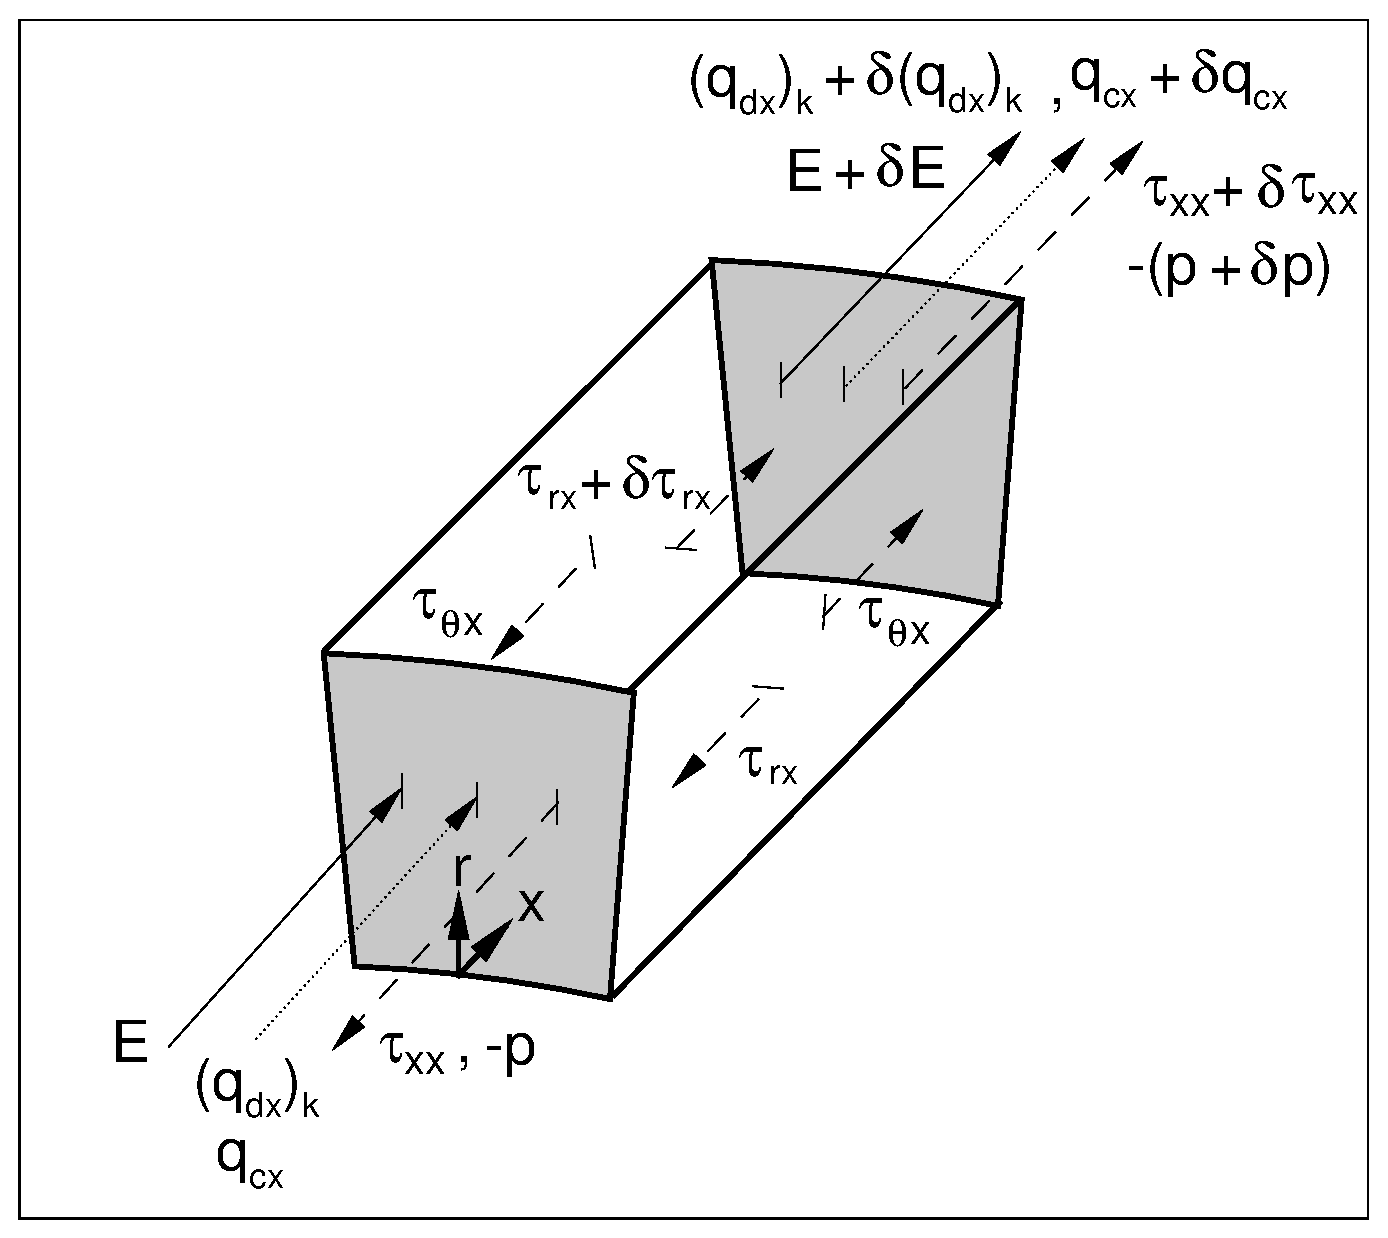
\includegraphics[height=5cm]{./xdirener.eps}
% One can specify [angle=x,width=y,height=z] for the graphics
\caption[$r$ - $\theta$ planes]{$r$ - $\theta$ planes : Energy itself is depicted by a solid line, forces  
				acting on the infantesimal fluid element are depicted by dashed lines (these
				are the same forces as in Fig. \ref{fig:xdir}) and the sources of energy
				transfer are depicted by dotted lines)}
\label{fig:xdirener}
\end{figure}

	For a infantesimal fluid volume in motion, the total energy is composed of internal energy, $\rho e$,
(where $e$ is the specific internal energy) and the kinetic energy due to motion $\frac{1}{2}\rho\vec{V}^2$.  
If $E$ represents the total \emph{specific} energy then

\begin{equation}
	E = e + \frac{1}{2}\vec{V}^2 
\label{eqn:spenergy}
\end{equation}

	From Fig. \ref{fig:xdirener} one can write

\begin{displaymath}
	\begin{array}{ccc}
		\textrm{Total Energy in the front $r$ - $\theta$ plane} & = & 
		(\rho E)u dr(R_o \theta) \\ & & \\
		\textrm{Total Energy out the back $r$ - $\theta$ plane} & = &
		(\rho E + \frac{\partial \rho E}{\partial x}dx)(u + \frac{\partial u}{\partial x}dx)dr(R_o \theta)
	\end{array}
\end{displaymath}	

	and from Fig. \ref{fig:rdirener}

\begin{displaymath}
	\begin{array}{ccc}
		\textrm{Total Energy in the bottom $x$ - $\theta$ plane} & = & 
		(\rho E)v dx(R_o \theta) \\ & & \\
		\textrm{Total Energy out the top $x$ - $\theta$ plane} & = &
		(\rho E + \frac{\partial \rho E}{\partial r}dr)(v + \frac{\partial v}{\partial r}dr)dx(R_o + dr)\theta
	\end{array}
\end{displaymath}

	Taking the net difference between the outflow and inflow and allowing for an unsteady change in the total energy
yields,

\begin{displaymath}
	\begin{array}{ccc}
		\begin{array}{c}
		\textrm{Rate of Change} \\ \textrm{of Total} \\ \textrm{Energy Inside} \\ \textrm{Infantesimal Volume}
		\end{array} & = &
		\begin{array}{c}
		(\rho E u dr + \rho E \frac{\partial u}{\partial x}dxdr + u \frac{\partial \rho E}{\partial x}dxdr +
		\frac{\partial u}{\partial x} \frac{\partial \rho E}{\partial x}dx^2dr - \rho E u dr + \rho E v dx \\
		+ \rho E \frac{\partial v}{\partial r}dxdr + v \frac{\partial \rho E}{\partial r}dxdr +
		\frac{\partial v}{\partial r} \frac{\partial \rho E}{\partial r}dxdr^2 - \rho E v dx  + \frac{\partial \rho E}
		{\partial t}dxdr)(R_o \theta) \\
		(\rho E v + \rho E \frac{\partial v}{\partial r}dr + v \frac{\partial \rho E}{\partial r}dr +
		\frac{\partial \rho E}{\partial r}\frac{\partial v}{\partial r}dr^2)dxdr \theta
		\end{array}
	\end{array}
\end{displaymath}

	After cancelling like terms and neglecting triple products and higher of differentials the above simplifies to

\begin{displaymath}
	\begin{array}{ccc}
		\begin{array}{c}
		\textrm{Rate of Change of Total Energy} \\ \textrm{Inside Infantesimal Volume}
		\end{array} & = &
		\Big\{( \frac{\partial \rho E}{\partial t} +\frac{\partial \rho E u}{\partial x} + \frac{\partial \rho E v}
		{\partial r})(R_o \theta) + (\rho E v)\theta \Big\}dxdr
	\end{array}
\end{displaymath}

	which after eliminating $\theta$ using Eq.\ref{eqn:theta} yields

\begin{equation}
	\begin{array}{ccc}
		\begin{array}{c}
		\textrm{Rate of Change of Total Energy} \\ \textrm{Inside Infantesimal Volume}
		\end{array} & = &
		\Big\{\frac{\partial \rho E}{\partial t} +\frac{\partial \rho E u}{\partial x} + \frac{\partial \rho E v}
		{\partial r} + \frac{1}{r}(\rho E v)\Big\}dxdr
	\end{array}
\label{eqn:energychange}
\end{equation}

\begin{figure}[hb]
\includegraphics[height=5cm]{./rdirener.eps}
% One can specify [angle=x,width=y,height=z] for the graphics
\caption[$r$ - $\theta$ planes]{$r$ - $\theta$ planes : Energy itself is depicted by a solid line, forces  
				acting on the infantesimal fluid element are depicted by dashed lines (these
				are the same forces as in Fig. \ref{fig:rdir}) and the sources of energy
				transfer are depicted by dotted lines)}
\label{fig:rdirener}
\end{figure}

\subsubsection{Energy Transfer due to Species Diffusion}

	Considering first species diffusion, from Eq.\ref{eqn:fick} one already has an expression for the rate
at which species diffusion occurs (as the units of the diffusive flux, $j_{k_x}$, are $kg/m^2 s$).  Hence to calculate the 
energy transfer occuring due to this flux, one needs only a quantity for the energy of the given species \emph{k}
per unit mass of species \emph{k}.  The specific enthalpy of a given species \emph{k}, $h_k$, has units of
$J/kg$ and is thus a suitable quanitity for determining the energy transfer due to species diffusion.  Therefore,

\begin{displaymath}
	\begin{array}{ccccc}
		\begin{array}{c}
			\textrm{Energy transfer due to species}\\ \textrm{diffusion in the $x$ direction}
		\end{array} 
		& = & (q_{d_x})_k & = & j_{k_x}h_k
		\\ & & & & \\
		\begin{array}{c}
			\textrm{Energy transfer due to species}\\ \textrm{diffusion in the $r$ direction} 
		\end{array}
		& = & (q_{d_r})_k & = & j_{k_r}h_k
	\end{array}
\end{displaymath} 

	which after substituting the results of Eqs. \ref{eqn:fick} and \ref{eqn:nuk} yields,

\begin{equation}
	(q_{d_x})_k = -\nu_k \frac{\partial c_k}{\partial x}h_k
\label{eqn:qdx}
\end{equation}

\begin{equation}
	(q_{d_r})_k = -\nu_k \frac{\partial c_k}{\partial r}h_k
\label{eqn:qdr}
\end{equation}

	Now, considering this energy flow in the $x$ direction first, as shown in Fig. \ref{fig:xdirener}, and
remembering to sum the total energy transfer over all the species \emph{k} present in the flow

\begin{displaymath}
	\begin{array}{ccc}
		\textrm{Energy in the front $r$ - $\theta$ plane} & = & \sum_k (q_{d_x})_kdr(R_o \theta) 
		\\ & & \\
		\textrm{Energy out the back $r$ - $\theta$ plane} & = & -\Big\{\sum_k (q_{d_x})_k + 
		\frac{\partial \sum_k (q_{d_x})_k}{\partial x}dx\Big\}dr(R_o \theta)
	\end{array}
\end{displaymath}

	while in the $r$ direction,

\begin{displaymath}
	\begin{array}{ccc}
		\textrm{Energy in the bottom $x$ - $\theta$ plane} & = & \sum_k (q_{d_r})_kdx(R_o \theta) 
		\\ & & \\
		\textrm{Energy out the top $x$ - $\theta$ plane} & = & -\Big\{\sum_k (q_{d_r})_k + 
		\frac{\partial \sum_k (q_{d_r})_k}{\partial r}dr\Big\}dx(R_o + dr) \theta
	\end{array}
\end{displaymath}

	Taking the sum of these quantities yields,

\begin{displaymath}
	\begin{array}{ccc}
		\begin{array}{c}
		\textrm{Net Energy Transfer} \\ \textrm{due to Species Diffusion}
		\end{array} & = &
			\begin{array}{c}
		\Big\{\sum_k (q_{d_x})_kdr - \sum_k (q_{d_x})_kdr - \frac{\partial \sum_k (q_{d_x})_k}{\partial x}dxdr \\
		+  \sum_k (q_{d_r})_kdx - \sum_k (q_{d_r})_kdx - \frac{\partial \sum _k(q_{d_r})_k}{\partial r}dxdr\Big\}
		(R_o \theta)\\
		\Big\{-\sum_k (q_{d_r})_k - \frac{\partial \sum_k (q_{d_r})_k}{\partial r}dr\Big\}dxdr \theta
			\end{array}
	\end{array}
\end{displaymath}

	which after simplifying, substituting Eq.\ref{eqn:theta} and neglecting triple products of differentials reduces to

\begin{equation}
	\begin{array}{ccc}
	\begin{array}{c}
	\textrm{Net Energy Transfer} \\ \textrm{due to Species Diffusion}
	\end{array} & = &
		\begin{array}{c}
			\Big\{-\frac{\partial \sum_k (q_{d_x})_k}{\partial x} - \frac{\partial \sum_k (q_{d_r})_k}{\partial r}
			- \frac{1}{r} \sum_k (q_{d_r})_k \Big\}dxdr	
		\end{array}
	\end{array}
\label{eqn:diff}
\end{equation}

	Combining the results of Eqs.\ref{eqn:energychange} and \ref{eqn:diff} and substituting Eqs.\ref{eqn:qdx} and
\ref{eqn:qdr}

\begin{displaymath}
	\begin{array}{ccc}
		\Big\{\frac{\partial \rho E}{\partial t} +\frac{\partial \rho E u}{\partial x} + \frac{\partial \rho E v}
		{\partial r} + \frac{1}{r}(\rho E v)\Big\}dxdr & = &
		\begin{array}{c}
			\Big\{\frac{\partial \sum_k (\nu_k \frac{\partial c_k}{\partial x}h_k)}{\partial x} 
			+ \frac{\partial \sum_k (\nu_k \frac{\partial c_k}{\partial r}h_k)}{\partial r}
			+ \frac{1}{r} \sum_k (\nu_k \frac{\partial c_k}{\partial r}h_k) + \ldots \Big\}dxdr	
		\end{array} 
	\end{array}
\end{displaymath}

\subsubsection{Energy Transfer due to Heat}

	The transfer of energy by heat follows the same logic as the transfer of energy by diffusion, only the
heat fluxes, $(q_c)_x$ and $(q_c)_r$ are defined by

\begin{equation}
	q_{c_x} = -\kappa \frac{\partial T}{\partial x} 
\label{eqn:xheatflux}
\end{equation}

\begin{equation}
	q_{c_r} = -\kappa \frac{\partial T}{\partial r}
\label{eqn:rheatflux}
\end{equation}	

	whose units are $J/m^2 s$ and where $k$ is the coefficient of thermal conductivity for the fluid 
as a whole (which can be found using a suitable mixing rule over all the individual species).  Thus for the $x$
direction

\begin{displaymath}
	\begin{array}{ccc}
		\textrm{Energy in the front $r$ - $\theta$ plane} & = & q_{c_x}dr(R_o \theta) 
		\\ & & \\
		\textrm{Energy out the back $r$ - $\theta$ plane} & = & -(q_{c_x} + 
		\frac{\partial q_{c_x}}{\partial x}dx)dr(R_o \theta)
	\end{array}
\end{displaymath}

	while in the $r$ direction,

\begin{displaymath}
	\begin{array}{ccc}
		\textrm{Energy in the bottom $x$ - $\theta$ plane} & = & q_{c_r}dx(R_o \theta) 
		\\ & & \\
		\textrm{Energy out the top $x$ - $\theta$ plane} & = & -(q_{c_r} + \frac{\partial q_{c_r}}
		{\partial r}dr)dx(R_o + dr) \theta
	\end{array}
\end{displaymath}

	Taking the sum of these quantities yields,

\begin{displaymath}
	\begin{array}{ccc}
		\begin{array}{c}
		\textrm{Net Energy Transfer} \\ \textrm{due to Heat}
		\end{array} & = &
			\begin{array}{c}
		q_{c_x}dr - q_{c_x}dr - \frac{\partial q_{c_x}}{\partial x}dxdr \\
		+  q_{c_r}dx - q_{c_r}dx - \frac{\partial q_{c_r}}{\partial r}dxdr)(R_o \theta)
		\\
		\Big\{-q_{c_r} - \frac{\partial q_{c_r}}{\partial r}dr\Big\}dxdr \theta
			\end{array}
	\end{array}
\end{displaymath}

	which after simplifying, substituting Eq.\ref{eqn:theta} and neglecting triple products of differentials reduces to

\begin{equation}
	\begin{array}{ccc}
	\begin{array}{c}
	\textrm{Net Energy Transfer} \\ \textrm{due to Heat}
	\end{array} & = &
		\begin{array}{c}
			(- \frac{\partial q_{c_x}}{\partial x} - \frac{\partial q_{c_r}}{\partial r}
			- \frac{1}{r} q_{c_r})dxdr
		\end{array}
	\end{array}
\label{eqn:heat}
\end{equation}

	Combining these results with those from Eqs.\ref{eqn:energychange},\ref{eqn:diff}, and \ref{eqn:heat}

\begin{displaymath}
	\begin{array}{ccc}
		\Big\{\frac{\partial \rho E}{\partial t} +\frac{\partial \rho E u}{\partial x} + \frac{\partial \rho E v}
		{\partial r} + \frac{1}{r}(\rho E v)\Big\}dxdr & = &
		\begin{array}{c}
			\Big\{\frac{\partial \sum_k (\nu_k \frac{\partial c_k}{\partial x}h_k)}{\partial x} 
			+\frac{\partial \sum_k (\nu_k \frac{\partial c_k}{\partial r}h_k)}{\partial r}
			-\frac{\partial q_{c_x}}{\partial x} - \frac{\partial q_{c_r}}{\partial r} \\
			+\frac{1}{r}[\sum_k (\nu_k \frac{\partial c_k}{\partial r}h_k) - q_{c_r}] + \ldots \Big\}dxdr	
		\end{array}  
	\end{array}
\end{displaymath}

\subsubsection{Rate of Work Done}

	Work is often expressed as the product of force and distance, where both these
quantities act parallel to one another.  However, for force and distance vectors in general (i.e., not necessarily
parallel) work can be expressed in integral form as,

\begin{displaymath}
	\begin{array}{ccc}
		W & = & \int_{s_0}^{s_1} \vec{F} \cdot \vec{ds}
	\end{array}
\end{displaymath}

	and hence the rate of work done (per unit time, $\dot{W}=\frac{\partial W}{\partial t}$) can be expressed as
\begin{equation}
	\dot{W} = \vec{F} \cdot \vec{V}
\label{eqn:dworkdt}
\end{equation}

	where the dot product of the force and velocity vectors can be expressed as

\begin{equation}
	\vec{F} \cdot \vec{V} = \mid F \mid \cos \theta \mid V \mid
\label{eqn:workdotproduct}
\end{equation}

	Thus when the force is parallel to the velocity, $\cos (0^o) = 1$, while for perpendicular vectors
there is no work done as $\cos (90^o) = 0$.  So, starting with the forces acting in the $x$ direction as shown
in Fig. \ref{fig:xdirener}

\begin{displaymath}
	\begin{array}{ccc}
	   \begin{array}{c}
		\textrm{Work due to pressure acting} \\ \textrm{on the front $r$ - $\theta$ plane}
	   \end{array} & = &
	(pu)dr(R_o \theta)
	\\ & & \\
	   \begin{array}{c}
		\textrm{Work due to pressure acting} \\ \textrm{on the back $r$ - $\theta$ plane}
	   \end{array} & = &
	-(p + \frac{\partial p}{\partial x}dx)(u + \frac{\partial u}{\partial x}dx)dr(R_o \theta)
	\\ & & \\
	   \begin{array}{c}
		\textrm{Work due to shear acting} \\ \textrm{on the front $r$ - $\theta$ plane}
	   \end{array} & = &
	-(\tau_{xx}u)dr(R_o \theta)
	\\ & & \\
	   \begin{array}{c}
		\textrm{Work due to shear acting} \\ \textrm{on the back $r$ - $\theta$ plane}
	   \end{array} & = &
	(\tau_{xx} + \frac{\partial \tau_{xx}}{\partial x}dx)(u + \frac{\partial u}{\partial x}dx)dr(R_o \theta)
	\\ & & \\
	   \begin{array}{c}
		\textrm{Work due to shear acting} \\ \textrm{on the bottom $x$ - $\theta$ plane}
	   \end{array} & = &
	-(\tau_{rx}u)dx(R_o \theta)
	\\ & & \\
	   \begin{array}{c}
		\textrm{Work due to shear acting} \\ \textrm{on the top $x$ - $\theta$ plane}
	   \end{array} & = &
	(\tau_{rx} + \frac{\partial \tau_{rx}}{\partial r}dr)(u + \frac{\partial u}{\partial r}dr)dx(R_o + dr) \theta
	\end{array}
\end{displaymath}
	
	It is noted here that the work done by the parallel shears ($\tau_{\theta x}$) is zero due to the axisymmetric
condition expressed in Eq.\ref{eqn:dtheta}.  Summing all the above quantities yields the total work done on the 
fluid element by the forces acting in the $x$ direction

\begin{displaymath}
	\begin{array}{ccc}
		\Delta \dot{W}_x & = &
			\begin{array}{c} 
		(-p udr - p \frac{\partial u}{\partial x}dxdr - u \frac{\partial p}{\partial x}dxdr - 
		\frac{\partial p}{\partial x} \frac{\partial u}{\partial x}dx^2dr + pudr \\
		+ \tau_{xx}udr + \tau_{xx} \frac{\partial u}{\partial x}dxdr + u \frac{\partial \tau_{xx}}{\partial x}dxdr
		+ \frac{\partial \tau_{xx}}{\partial x} \frac{\partial u}{\partial x} dx^2dr - \tau_{xx}udr \\
		+ \tau_{rx}udx + \tau_{rx} \frac{\partial u}{\partial r}dxdr + u \frac{\partial \tau_{rx}}{\partial r}dxdr
		+ \frac{\partial \tau_{rx}}{\partial r} \frac{\partial u}{\partial r} dxdr^2 - \tau_{rx}udx)	
		(R_o \theta) \\
		+ (\tau_{rx}u + \tau_{rx} \frac{\partial u}{\partial r}dr + u \frac{\partial \tau_{rx}}{\partial r}dr
		+ \frac{\partial \tau_{rx}}{\partial r} \frac{\partial u}{\partial r} dr^2)dxdr \theta
			\end{array}
	\end{array}
\end{displaymath}

	which when simplified and combined with the relation expressed in Eq.\ref{eqn:theta} yields,

\begin{displaymath}
	\begin{array}{ccc}
		\Delta \dot{W}_x & = &
			\begin{array}{c} 
		\Big\{-\frac{\partial pu}{\partial x} + \frac{\partial \tau_{xx}u}{\partial x}
		+ \frac{\partial \tau_{rx}u}{\partial r} + \frac{1}{r}(\tau_{rx}u)\Big\}dxdr 
			\end{array}
	\end{array}
\end{displaymath}

	Next considering the forces in the $r$ direction as shown in Fig. \ref{fig:rdirener}

\begin{displaymath}
	\begin{array}{ccc}
	   \begin{array}{c}
		\textrm{Work due to pressure acting} \\ \textrm{on the bottom $x$ - $\theta$ plane}
	   \end{array} & = &
	(pv)dx(R_o \theta)
	\\ & & \\
	   \begin{array}{c}
		\textrm{Work due to pressure acting} \\ \textrm{on the top $x$ - $\theta$ plane}
	   \end{array} & = &
	-(p + \frac{\partial p}{\partial r}dr)(v + \frac{\partial v}{\partial r}dr)dx(R_o + dr) \theta
	\\ & & \\
	   \begin{array}{c}
		\textrm{Work due to shear acting} \\ \textrm{on the bottom $x$ - $\theta$ plane}
	   \end{array} & = &
	-(\tau_{rr}v)dx(R_o \theta)
	\\ & & \\
	   \begin{array}{c}
		\textrm{Work due to shear acting} \\ \textrm{on the top $x$ - $\theta$ plane}
	   \end{array} & = &
	(\tau_{rr} + \frac{\partial \tau_{rr}}{\partial r}dr)(v + \frac{\partial v}{\partial r}dr)dx(R_o + dr) \theta
	\\ & & \\
	   \begin{array}{c}
		\textrm{Work due to shear acting} \\ \textrm{on the front $r$ - $\theta$ plane}
	   \end{array} & = &
	-(\tau_{xr}v)dr(R_o \theta)
	\\ & & \\
	   \begin{array}{c}
		\textrm{Work due to shear acting} \\ \textrm{on the back $r$ - $\theta$ plane}
	   \end{array} & = &
	(\tau_{xr} + \frac{\partial \tau_{xr}}{\partial x}dx)(v + \frac{\partial v}{\partial x}dx)dr(R_o \theta)
	\end{array}
\end{displaymath}

	As was the case for the $r$ momentum equation, by symmetry, it can be see that since $\tau_{\theta r}$ 
acts in opposite directions and on opposite faces of the fluid element, it's net effect in the $r$ direction will
be zero due to the axisymmetric condtion expressed by Eq.\ref{eqn:dtheta}.  The argument for neglecting the contribution both the shear force ($\tau_{\theta \theta}$) and pressure make in the $r$
directions is directly related to the definition of $\dot{W}$ in Eq.\ref{eqn:workdotproduct}.  Since both these forces
by definition are perpendicular to the surface upon which they act, the dot product is zero and hence no work can be
done by these forces in the $r$ direction.  Therefore, summing the other contributions to the work done in the $r$ 
direction yields (while also applying	the relation expressed in Eq.\ref{eqn:smallangle}),

\begin{displaymath}
	\begin{array}{ccc}
		\Delta \dot{W}_r & = &
			\begin{array}{c} 
		(-p vdx - p \frac{\partial v}{\partial r}dxdr - v \frac{\partial p}{\partial r}dxdr 
		- \frac{\partial p}{\partial r} \frac{\partial v}{\partial x}dxdr^2 + p vdx \\
		+ \tau_{rr}vdx + \tau_{rr} \frac{\partial v}{\partial r}dxdr + v \frac{\partial \tau_{rr}}{\partial r}dxdr
		+ \frac{\partial \tau_{rr}}{\partial r} \frac{\partial v}{\partial r} dxdr^2 - \tau_{rr}vdr \\
		+ \tau_{xr}vdr + \tau_{xr} \frac{\partial v}{\partial x}dxdr + v \frac{\partial \tau_{xr}}{\partial x}dxdr
		+ \frac{\partial \tau_{xr}}{\partial x} \frac{\partial v}{\partial x} dx^2dr - \tau_{xr}vdr)	
		(R_o \theta) \\
		(-p v - p \frac{\partial v}{\partial r}dr - v \frac{\partial p}{\partial r}dr 
		- \frac{\partial p}{\partial r} \frac{\partial v}{\partial x}dr^2 \\
		+ \tau_{rr}v + \tau_{rr} \frac{\partial v}{\partial r}dr + v \frac{\partial \tau_{rr}}{\partial r}dr
		+ \frac{\partial \tau_{rr}}{\partial r} \frac{\partial v}{\partial r} dr^2)dxdr \theta
			\end{array}
	\end{array}
\end{displaymath}

	which when simplified and combined with the relation expressed in Eq.\ref{eqn:theta} yields,

\begin{displaymath}
	\begin{array}{ccc}
		\Delta \dot{W}_r & = &
			\begin{array}{c} 
		\Big\{-\frac{\partial pv}{\partial r} + \frac{\partial \tau_{rr}v}{\partial r}
		+ \frac{\partial \tau_{xr}v}{\partial x} + \frac{1}{r}(\tau_{rr}v -p v)\Big\}dxdr 
			\end{array}
	\end{array}
\end{displaymath}

	Combining the results from both the $x$ and $r$ directions

\begin{displaymath}
	\begin{array}{ccc}
		\textrm{Net Rate of Work Done} & = & \Delta \dot{W}_x + \Delta \dot{W}_r 
	\end{array}
\end{displaymath}

\begin{equation}
	\begin{array}{c}
	\textrm{Net Rate}\\ \textrm{of Work Done}
	\end{array} =  
			\begin{array}{c} 
		\Big\{-\frac{\partial pu}{\partial x}  
		+ \frac{\partial \tau_{xx}u}{\partial x}
		+ \frac{\partial \tau_{rx}u}{\partial r} + \frac{1}{r}(\tau_{rx}u) -\frac{\partial pv}{\partial r}
		+ \frac{\partial \tau_{xr}v}{\partial x} + \frac{\partial \tau_{rr}v}{\partial r} 
		+ \frac{1}{r}(\tau_{rr}v -pv)\Big\}dxdr 
			\end{array}	
\label{eqn:work}
\end{equation}

	Combining the results of Eqs.\ref{eqn:energychange},\ref{eqn:diff},\ref{eqn:heat}, and \ref{eqn:work} yields,

\begin{displaymath}
	\begin{array}{ccc}
		\Big\{\frac{\partial \rho E}{\partial t} +\frac{\partial \rho E u}{\partial x} + \frac{\partial \rho E v}
		{\partial r} + \frac{1}{r}(\rho E v)\Big\}dxdr & = &
		\begin{array}{c}
			\Big\{-\frac{\partial pu}{\partial x} -\frac{\partial pv}{\partial r}
			+\frac{\partial \sum_k (\nu_k \frac{\partial c_k}{\partial x}h_k)}{\partial x} 
			+ \frac{\partial \sum_k (\nu_k \frac{\partial c_k}{\partial r}h_k)}{\partial r}
			 \\
			-\frac{\partial q_{c_x}}{\partial x} - \frac{\partial q_{c_r}}{\partial r}
			+ \frac{\partial \tau_{xx}u}{\partial x} + \frac{\partial \tau_{rx}u}{\partial r} 
			+ \frac{\partial \tau_{xr}v}{\partial x} + \frac{\partial \tau_{rr}v}{\partial r} \\
			+\frac{1}{r}[\sum_k (\nu_k \frac{\partial c_k}{\partial r}h_k) - q_{c_r} + \tau_{rx}u 
			+ \tau_{rr}v - pv] + \ldots \Big\}dxdr	
		\end{array}  
	\end{array}	
\end{displaymath}

\subsubsection{Energy Transfer due to Turbulence Diffusion}

	Leaving the actual derivation of the terms used to model turbulence for the moment, it is possible if one 
accepts the various terms required, to incorporate them (where required) into the axisymmetric Navier-Stokes equations
currently under consideration (although it is noted that to be perfectly accurate, once turbulence is added to the
Navier-Stokes equations they then represent a given type of averaged quantities and hence are called, for example, the
Favre-Averaged Navier-Stokes equations).  If one models turbulence using a $k$ - $\omega$ model, these two quantities 
represent the specific turbulent kinetic energy (TKE) and a specific length scale parameter (relating the kinetic energy of 
turbulence to the rate at which it dissipates) respectively.  Since $k$ represents a type of energy (it has units of 
$J/kg$), it is natural that it would have an effect on the overall energy equation.  Treating $k$ as a flow property similar 
to $\rho_k$ in that a TKE gradient will cause diffusion one can write 

\begin{equation}
	\begin{array}{ccccc}
		\textrm{Energy transfer due to turbulence}\\ \textrm{diffusion in the $x$ direction} & = &
		z_x & = & -{\mu _k}^* \frac{\partial k}{\partial x}
	\end{array}
\label{eqn:zx}
\end{equation}

\begin{equation}
	\begin{array}{ccccc}
		\textrm{Energy transfer due to turbulence}\\ \textrm{diffusion in the $r$ direction} & = &
		z_r & = & -{\mu _k}^* \frac{\partial k}{\partial r}
	\end{array}
\label{eqn:zr}
\end{equation}

	where ${\mu_k}^*$ is the coefficient of diffusion for the turbulent kinetic energy (Note that $z_x$ and $z_r$ 
have units of $J/m^2 s$).  

\begin{displaymath}
	\begin{array}{ccc}
		\textrm{Energy in the front $r$ - $\theta$ plane} & = & z_xdr(R_o \theta) 
		\\ & & \\
		\textrm{Energy out the back $r$ - $\theta$ plane} & = & -(z_x + 
		\frac{\partial z_x}{\partial x}dx)dr(R_o \theta)
	\end{array}
\end{displaymath}

	while in the $r$ direction,

\begin{displaymath}
	\begin{array}{ccc}
		\textrm{Energy in the bottom $x$ - $\theta$ plane} & = & z_rdx(R_o \theta) 
		\\ & & \\
		\textrm{Energy out the top $x$ - $\theta$ plane} & = & -(z_r + 
		\frac{\partial z_r}{\partial r}dr)dx(R_o + dr) \theta
	\end{array}
\end{displaymath}

	Taking the sum of these quantities yields,

\begin{displaymath}
	\begin{array}{ccc}
		\begin{array}{c}
		\textrm{Net Energy Transfer} \\ \textrm{due to Turbulence Diffusion}
		\end{array} & = &
			\begin{array}{c}
		z_xdr - z_xdr - \frac{\partial z_x}{\partial x}dxdr \\
		+  z_rdx - z_rdx - \frac{\partial z_r}{\partial r}dxdr)(R_o \theta)
		\\
		\Big\{-z_r - \frac{\partial z_r}{\partial r}dr\Big\}dxdr \theta
			\end{array}
	\end{array}
\end{displaymath}

	which after simplifying, substituting Eq.\ref{eqn:theta} and neglecting triple products of differentials reduces to

\begin{displaymath}
	\begin{array}{ccc}
	\begin{array}{c}
	\textrm{Net Energy Transfer} \\ \textrm{due to Turbulence Diffusion}
	\end{array} & = &
		\begin{array}{c}
			\Big\{-\frac{\partial z_x}{\partial x} - \frac{\partial z_r}{\partial r}
			- \frac{1}{r} z_r\Big\}dxdr
		\end{array}
	\end{array}
\end{displaymath}

	Substituting Eqs.\ref{eqn:zx} and \ref{eqn:zr} into the above,

\begin{equation}
	\begin{array}{ccc}
	\begin{array}{c}
	\textrm{Net Energy Transfer} \\ \textrm{due to Turbulence Diffusion}
	\end{array} & = &
		\begin{array}{c}
			\Big\{\frac{\partial ({\mu_k}^* \frac{\partial k}{\partial x})}{\partial x} 
			+ \frac{\partial ({\mu_k}^* \frac{\partial k}{\partial r})}{\partial r}
			+ \frac{1}{r} ({\mu_k}^* \frac{\partial k}{\partial r})\Big\}dxdr
		\end{array}
	\end{array}
\label{eqn:turb}
\end{equation}

	Combining the results of Eqs.\ref{eqn:energychange},\ref{eqn:diff},\ref{eqn:heat},\ref{eqn:work}, and \ref{eqn:turb} 
yields,

\begin{equation}
	\begin{array}{ccc}
		\Big\{\frac{\partial \rho E}{\partial t} +\frac{\partial \rho E u}{\partial x} + \frac{\partial \rho E v}
		{\partial r} + \frac{1}{r}(\rho E v)\Big\}dxdr & = &
		\begin{array}{c}
			\Big\{-\frac{\partial pu}{\partial x} -\frac{\partial pv}{\partial r}
			+\frac{\partial \sum_k (\nu_k \frac{\partial c_k}{\partial x}h_k)}{\partial x} 
			+ \frac{\partial \sum_k (\nu_k \frac{\partial c_k}{\partial r}h_k)}{\partial r}
			-\frac{\partial q_{c_x}}{\partial x} - \frac{\partial q_{c_r}}{\partial r} \\
			+ \frac{\partial \tau_{xx}u}{\partial x} + \frac{\partial \tau_{rx}u}{\partial r} 
			+ \frac{\partial \tau_{xr}v}{\partial x} + \frac{\partial \tau_{rr}v}{\partial r} 
			+ \frac{\partial({\mu_k}^* \frac{\partial k}{\partial x})}{\partial x} 
			+ \frac{\partial ({\mu_k}^* \frac{\partial k}{\partial r})}{\partial r} \\
			+\frac{1}{r}[\sum_k (\nu_k \frac{\partial c_k}{\partial r}h_k) - q_{c_r} + \tau_{rx}u + \tau_{rr}v - pv
			+ {\mu_k}^* \frac{\partial k}{\partial r}]\Big\}dxdr	
		\end{array}  
	\end{array}	
\label{eqn:energyshear}
\end{equation}

	Using Eqs.\ref{eqn:tauxx} and \ref{eqn:taurr} one can write

\begin{displaymath}
	\tau_{xx}u = \hat \tau_{xx} u - \mu \frac{2}{3} \frac {uv}{r}  
\end{displaymath}

\begin{displaymath}
	\tau_{rr}v = \hat \tau_{rr} v - \mu \frac{2}{3} \frac {v^2}{r}
\end{displaymath}

	and thus the overall energy equation can be rewritten as

\begin{equation}
	\begin{array}{ccc}
		\begin{array}{c}
		\Big\{\frac{\partial}{\partial t}(\rho E) +\frac{\partial}{\partial x}(\rho E u + pu) \\
		+ \frac{\partial}{\partial r}(\rho E v + pv) + \frac{1}{r}(\rho E v + pv)\Big\}
		\end{array} & = &
		\begin{array}{c}
			\frac{\partial}{\partial x}\Big\{
			\sum_k (\nu_k \frac{\partial c_k}{\partial x}h_k) 
			- q_{c_x} +  \hat \tau_{xx}u + \tau_{xr}v + {\mu_k}^* \frac{\partial k}{\partial x}\Big\} \\
			\frac{\partial}{\partial r}\Big\{
			\sum_k (\nu_k \frac{\partial c_k}{\partial r}h_k)
			-  q_{c_r} + \hat \tau_{rr}v + \tau_{rx}u + {\mu_k}^* \frac{\partial k}{\partial r}\Big\} \\
			+\frac{1}{r}\Big\{\sum_k (\nu_k \frac{\partial c_k}{\partial r}h_k) - q_{c_r} + \tau_{rx}u 
			+ \hat \tau_{rr}v + {\mu_k}^* \frac{\partial k}{\partial r} - \frac{2}{3} \mu \frac{v^2}{r}\Big\} \\
			- \frac{2}{3} \frac{\partial}{\partial x}(\mu \frac{uv}{r})
			- \frac{2}{3} \frac{\partial}{\partial r}(\mu \frac{v^2}{r}) 
		\end{array}  
	\end{array}
\label{eqn:energy}
\end{equation}

%-------------------------------------------------------------------------------------------------------------------------
\subsection{Turbulent Kinetic Energy}

	The turbulent kinetic energy equation can be derived in a similar fashion to the species conservation
equation if one excepts the existence of a quantity called turbulent kinetic energy ($k$).  The derivation of the conservation
equation for this quantity is somewhat lengthy and requires that the governing equations be written for time averaged variables,
thereby allowing for turbulent fluctuations of the flow properties.  This entire process of rephrasing the governing equations
in turbulent form is not shown here but can be found in the later sections.  However, following the same logic as before while 
allowing for an additional source term, treating the turbulent kinetic energy as a conserved quantity (without worrying about
its origin for the time being) one can write for the $x$ direction,

\begin{displaymath}
	\begin{array}{ccc}
		\begin{array}{c}
			\textrm{Turbulent kinetic energy} \\ \textrm{in through the front $r$ - $\theta$ plane} 
		\end{array} & 
	= & (\rho k u)dr(R_o \theta) + z_x dr(R_o \theta)\\
	& \\ & \\
		\begin{array}{c}
			\textrm{Turbulent kinetic energy} \\ \textrm{out through the back $r$ - $\theta$ plane}
		\end{array} & 
	= & \begin{array}{c}
		(\rho k + \frac{\partial \rho k}{\partial x}dx)(u + \frac{\partial u}{\partial x}dx)dr(R_o \theta) \\
	+ (z_x + \frac{\partial z_x}{\partial x}dx)dr(R_o \theta)
		\end{array}
	\end{array}
\end{displaymath}

	In the above equations, $z_x$ is the diffusive flux caused by gradients existing in the turbulent kinetic
energy which give rise to movement of the given species in the dirction opposite the gradient
(Note that $z_x$ has units of $J/m^2 s$). All other terms are shown in Fig. \ref{fig:xdirener}.
Taking the difference between these two planes (outflow - inflow) yields,

\begin{displaymath}
	\Delta \rho k_x = \Big\{(\rho k u + z_x + \rho k \frac{\partial u}{\partial x}dx + u \frac{\partial \rho k}
	{\partial x}dx + \frac{\partial u}{\partial x} \frac{\partial \rho k}{\partial x}dx^2 + \frac{\partial z_x}
	{\partial x}dx) - (\rho k u + z_x)\Big\} dr(R_o \theta)
\end{displaymath}

	Simplifying the above yields,

\begin{displaymath}
	\Delta \rho k_x = \Big( \frac{\partial \rho k u}{\partial x} + \frac{\partial z_x}{\partial x}
	\Big)dxdr(R_o \theta)
\end{displaymath}

	Considering the $r$ direction next,

\begin{displaymath}
	\begin{array}{ccc}
		\begin{array}{c}
			\textrm{Turbulent kinetic energy} \\ \textrm{in through the bottom $x$ - $\theta$ plane} 
		\end{array} & 
	= & (\rho k v)dx(R_o \theta) + z_r dx(R_o \theta)\\
	& \\ & \\
		\begin{array}{c}
			\textrm{Turbulent kinetic energy} \\ \textrm{out through the top $x$ - $\theta$ plane}
		\end{array} & 
	= & \begin{array}{c}
		(\rho k + \frac{\partial \rho k}{\partial r}dr)(v + \frac{\partial v}{\partial r}dr)dx
		(R_o + dr) \theta  \\
	+ (z_r + \frac{\partial z_r}{\partial r}dr)dx (R_o + dr) \theta
		\end{array}
	\end{array}
\end{displaymath}

	Taking the difference between the outflow and inflow in the $r$ direction yields,

\begin{displaymath}
	\begin{array}{ccc}
	\Delta \rho k_r & = &
		\begin{array}{c} 
	\Big\{(\rho k v + z_r + \rho k \frac{\partial v}{\partial r}dr + v \frac{\partial \rho k}
	{\partial r}dr + \frac{\partial v}{\partial r} \frac{\partial \rho k}{\partial r}dr^2 + \frac{\partial z_r}
	{\partial r}dr) -\rho k v - z_r\Big\} dx(R_o \theta) \\
	+ (\rho k v + z_r + \rho k \frac{\partial v}{\partial r}dr + v \frac{\partial \rho k}
	{\partial r}dr + \frac{\partial v}{\partial r} \frac{\partial \rho k}{\partial r}dr^2 + \frac{\partial z_r}
	{\partial r}dr) dx dr \theta
		\end{array}
	\end{array}
\end{displaymath}

	Again neglecting triple products (and higher) of differentials, the above equation reduces to the following,

\begin{displaymath}
	\Delta \rho k_r = \Big( \frac{\partial \rho k v}{\partial r} + \frac{\partial z_r}{\partial r}
	\Big)dxdr(R_o \theta) + (\rho k v + z_r)dxdr\theta
\end{displaymath}

	Allowing for any unsteady change in $\rho k$, the sum of the fluxes in 
each of the co-ordinate directions plus this unsteady change must sum to the source term for the kinetic energy of
turbulence, which for the moment will be left as a generic source term ($S_k$) to be defined later.

\begin{displaymath}
	\begin{array}{ccc}
	\frac{\partial \rho k}{\partial t}dxdr(R_o \theta) + \Delta \rho k_x + \Delta \rho k_r & = & (S_k)dxdr \\
	\Big\{(\frac{\partial \rho k}{\partial t} + \frac{\partial \rho k u}{\partial x} 
	+ \frac{\partial z_x}{\partial x}
	+  \frac{\partial \rho k v}{\partial r} + \frac{\partial z_r}{\partial r})(R_o \theta) + 
	(\rho k v + z_r)\theta \Big\}dxdr & = & (S_k)dxdr
	\end{array}
\end{displaymath}

	Rearranging and substituting the results of Eqs.\ref{eqn:zx} and \ref{eqn:zr} in for the turbulence fluxes and
using Eq.\ref{eqn:theta} for $\theta$ yields,

\begin{equation}
	\frac{\partial}{\partial t}(\rho k) + \frac{\partial}{\partial x}(\rho k u) + \frac{\partial}{\partial r}(\rho k v)
	+ \frac {1}{r}(\rho k v) = \frac{\partial}{\partial x}({\mu_k}^* \frac{\partial k}{\partial x}) 
	+ \frac{\partial}{\partial r}({\mu_k}^* \frac{\partial k}{\partial r}) 
	+ \frac {1}{r}({\mu_k}^* \frac{\partial k}{\partial r}) + S_k
\label{eqn:tkefinal}
\end{equation}

%---------------------------------------------------------------------------------------------------------------------------
\subsection{Turbulence Dissipation Rate Equation}

	If one accepts the existence of this variable as a requirement to define the turbulent nature of the flow field,
and allows for the definition of a source term, $S_\omega$ without specifying its exact origin or definition at the moment,
then the overall conservation equation for this property can be derived in exactly the same manner as that for the 
turbulent kinetic energy.

\begin{displaymath}
	\begin{array}{ccc}
		\begin{array}{c}
			\textrm{Turbulence dissipation rate} \\ \textrm{in through the front $r$ - $\theta$ plane} 
		\end{array} & 
	= & (\rho \omega u)dr(R_o \theta) + l_x dr(R_o \theta)\\
	& \\ & \\
		\begin{array}{c}
			\textrm{Turbulence dissipation rate} \\ \textrm{out through the back $r$ - $\theta$ plane}
		\end{array} & 
	= & \begin{array}{c}
		(\rho \omega + \frac{\partial \rho \omega}{\partial x}dx)(u + \frac{\partial u}{\partial x}dx)dr(R_o \theta) \\
	+ (l_x + \frac{\partial l_x}{\partial x}dx)dr(R_o \theta)
		\end{array}
	\end{array}
\end{displaymath}

	In the above equations, $l_x$ is the flux caused by gradients existing in the turbulent kinetic energy dissipation 
rate, similar to those cause by gradients in the turbulent kinetic energy itself.

\begin{displaymath}
	\Delta \rho \omega_x = \Big\{(\rho \omega u + l_x + \rho \omega \frac{\partial u}{\partial x}dx + u \frac{\partial \rho \omega}
	{\partial x}dx + \frac{\partial u}{\partial x} \frac{\partial \rho \omega}{\partial x}dx^2 + \frac{\partial l_x}
	{\partial x}dx) - (\rho \omega u + l_x)\Big\} dr(R_o \theta)
\end{displaymath}

	Simplifying the above yields,

\begin{displaymath}
	\Delta \rho \omega_x = \Big( \frac{\partial \rho \omega u}{\partial x} + \frac{\partial l_x}{\partial x}
	\Big)dxdr(R_o \theta)
\end{displaymath}

	Considering the $r$ direction next,

\begin{displaymath}
	\begin{array}{ccc}
		\begin{array}{c}
			\textrm{Turbulence dissipation rate} \\ \textrm{in through the bottom $x$ - $\theta$ plane} 
		\end{array} & 
	= & (\rho \omega v)dx(R_o \theta) + l_r dx(R_o \theta)\\
	& \\ & \\
		\begin{array}{c}
			\textrm{Turbulence dissipation rate} \\ \textrm{out through the top $x$ - $\theta$ plane}
		\end{array} & 
	= & \begin{array}{c}
		(\rho \omega + \frac{\partial \rho \omega}{\partial r}dr)(v + \frac{\partial v}{\partial r}dr)dx
		(R_o + dr) \theta  \\
	+ (l_r + \frac{\partial l_r}{\partial r}dr)dx (R_o + dr) \theta
		\end{array}
	\end{array}
\end{displaymath}

	Taking the difference between the outflow and inflow in the $r$ direction yields,

\begin{displaymath}
	\begin{array}{ccc}
	\Delta \rho \omega_r & = &
		\begin{array}{c} 
	\Big\{(\rho \omega v + l_r + \rho \omega \frac{\partial v}{\partial r}dr + v \frac{\partial \rho \omega}
	{\partial r}dr + \frac{\partial v}{\partial r} \frac{\partial \rho \omega}{\partial r}dr^2 + \frac{\partial l_r}
	{\partial r}dr) -\rho \omega v - l_r\Big\} dx(R_o \theta) \\
	+ (\rho \omega v + l_r + \rho \omega \frac{\partial v}{\partial r}dr + v \frac{\partial \rho \omega}
	{\partial r}dr + \frac{\partial v}{\partial r} \frac{\partial \rho \omega}{\partial r}dr^2 + \frac{\partial l_r}
	{\partial r}dr) dx dr \theta
		\end{array}
	\end{array}
\end{displaymath}

	Again neglecting triple products (and higher) of differentials, the above equation reduces to the following,

\begin{displaymath}
	\Delta \rho \omega_r = \Big( \frac{\partial \rho \omega v}{\partial r} + \frac{\partial l_r}{\partial r}
	\Big)dxdr(R_o \theta) + (\rho \omega v + l_r)dxdr\theta
\end{displaymath}

	Allowing for any unsteady change in $\rho \omega$, the sum of the fluxes in 
each of the co-ordinate directions plus this unsteady change must sum to the source term for the dissipation rate of the 
kinetic energy of turbulence, which for the moment will be left as a generic source term ($S_\omega$) to be defined later.

\begin{displaymath}
	\begin{array}{ccc}
	\frac{\partial \rho \omega}{\partial t}dxdr(R_o \theta) + \Delta \rho \omega_x + \Delta \rho \omega_r & = 
	& (S_\omega)dxdr \\
	\Big\{(\frac{\partial \rho \omega}{\partial t} + \frac{\partial \rho \omega u}{\partial x} 
	+ \frac{\partial l_x}{\partial x}
	+  \frac{\partial \rho \omega v}{\partial r} + \frac{\partial l_r}{\partial r})(R_o \theta) + 
	(\rho \omega v + l_r)\theta \Big\}dxdr & = & (S_\omega)dxdr
	\end{array}
\end{displaymath}

	Rearranging and modelling $l_x$ and $l_r$ along the lines of $z_x$ and $z_r$ as in Eqs.\ref{eqn:zx} 
and \ref{eqn:zr} while using Eq.\ref{eqn:theta} for $\theta$ yields,

\begin{equation}
	\frac{\partial}{\partial t}(\rho \omega) + \frac{\partial}{\partial x}(\rho \omega u) 
	+ \frac{\partial}{\partial r}(\rho \omega v)
	+ \frac {1}{r}(\rho \omega v) = \frac{\partial}{\partial x}({\mu_\omega}^* \frac{\partial \omega}{\partial x}) 
	+ \frac{\partial}{\partial r}({\mu_\omega}^* \frac{\partial \omega}{\partial r}) 
	+ \frac {1}{r}({\mu_\omega}^* \frac{\partial \omega}{\partial r}) + S_\omega
\label{eqn:dissipationfinal}
\end{equation}

%-----------------------------------------------------------------------------------------------------------------------
\subsection{Summary}

	Since we now have the complete set of desired equations, the last step is to place these equations into a 
more convenient matrix form.  Thus, the overall set of equations can be expressed in the form

\begin{equation}
	\frac{\partial Q}{\partial t} + \frac{\partial E}{\partial x} + \frac{\partial F}{\partial r} + S_{be3D}
	-\frac{\partial E_v}{\partial x} - \frac{\partial F_v}{\partial r} - S_{be3D_v} = 0
\label{eqn:final}
\end{equation}

	where the main variable vector is defined as

\begin{equation}
	Q = \left[ \begin{array}{c}
		\rho_1 \\
		\vdots \\
		\rho_k \\
		\rho u \\
		\rho v \\
		\rho E \\
		\rho k \\
		\rho \omega
		   \end{array}
	    \right]
\label{eqn:finalQ}
\end{equation}

	the inviscid flux vectors as

\begin{equation}
  \begin{array}{ccccccc}
	E & = & \left[ \begin{array}{c}
		\rho_1 u \\
		\vdots \\
		\rho_k u \\
		\rho u^2 + p \\
		\rho uv \\
		(\rho E + p)u \\
		\rho k u \\
		\rho \omega u
		   \end{array}
	    \right] &
	&
	F & = & \left[ \begin{array}{c}
		\rho_1 v \\
		\vdots \\
		\rho_k v \\
		\rho uv \\
		\rho v^2 + p \\
		(\rho E + p)v \\
		\rho k v \\
		\rho \omega v
		   \end{array}
	    \right]
  \end{array}
\label{eqn:finalEF}
\end{equation}

	and the inviscid source term as

\begin{equation}
	S_{be3D} = \frac{1}{r}\left[ \begin{array}{c}
		\rho_1 v \\
		\vdots \\
		\rho_k v \\
		\rho uv \\
		\rho v^2 \\
		(\rho E + p)v \\
		\rho k v \\
		\rho \omega v
		   \end{array}
	    \right]
\label{eqn:finalH}
\end{equation}

	The viscous terms flux terms are defined as 

\begin{equation}
  \begin{array}{ccc}
	E_v & = & \left[ \begin{array}{c}
		\mu_1 \frac{\partial c_1}{\partial x} \\
		\vdots \\
		\mu_k \frac{\partial c_k}{\partial x}  \\
		\hat{\tau}_{xx} \\
		\tau_{xr} \\
		\sum_k (\nu_k \frac{\partial c_k}{\partial x}h_k) 
			- q_{c_x} +  \hat \tau_{xx}u + \tau_{xr}v + {\mu_k}^* \frac{\partial k}{\partial x} \\
		{\mu_k}^* \frac{\partial k}{\partial x} \\
		{\mu_\omega}^* \frac{\partial \omega}{\partial x} \\
		   \end{array}
	    \right] 
	\\ & & \\
	F_v & = & \left[ \begin{array}{c}
		\mu_1 \frac{\partial c_1}{\partial r} \\
		\vdots \\
		\mu_k \frac{\partial c_k}{\partial r} \\
		\tau_{rx} \\
		\hat{\tau}_{rr} \\
		\sum_k (\nu_k \frac{\partial c_k}{\partial r}h_k)
			-  q_{c_r} + \hat \tau_{rr}v + \tau_{rx}u + {\mu_k}^* \frac{\partial k}{\partial r}\\
		{\mu_k}^* \frac{\partial k}{\partial r} \\
		{\mu_\omega}^* \frac{\partial \omega}{\partial r} \\
		   \end{array}
	    \right]
  \end{array}
\label{eqn:finalEvFv}
\end{equation}

	and finally the viscous source term can be written as,

\begin{equation}
	S_{be3D_v} = \frac{1}{r}\left[ \begin{array}{c}
		\nu_1 \frac{\partial c_1}{\partial r} \\
		\vdots \\
		\nu_k \frac{\partial c_k}{\partial r} \\
		\tau_{rx} - r\frac{2}{3}\frac{\partial}{\partial x}(\mu \frac{v}{r}) \\
		\hat{\tau}_{rr} -\tau_{\theta \theta} - \frac{2}{3}\mu \frac{v}{r} 
		- r\frac{2}{3}\frac{\partial}{\partial r}(\mu \frac{v}{r}) \\
		\sum_k (\nu_k \frac{\partial c_k}{\partial r}h_k) - q_{c_r} + \tau_{rx}u 
		+ \hat \tau_{rr}v + {\mu_k}^* \frac{\partial k}{\partial r} - \frac{2}{3} \mu \frac{v^2}{r}
			- r\frac{2}{3} \frac{\partial}{\partial x}(\mu \frac{uv}{r})
			- r\frac{2}{3} \frac{\partial}{\partial r}(\mu \frac{v^2}{r}) \\
		{\mu_k}^* \frac{\partial k}{\partial r} + rS_k\\
		{\mu_\omega}^* \frac{\partial \omega}{\partial r} + rS_\omega
		   \end{array}
	    \right]
\label{eqn:finalHv}
\end{equation}


\section{Axisymmetric Favre-Averaged Navier-Stokes Equations}
\subsection{Overview of Averaging Properties}

	The difference between the laminar multi-species axisymmetric equations already derived and expressed in 
Eqs.\ref{eqn:speciesfinal},\ref{eqn:xmom},\ref{eqn:rmom}, and \ref{eqn:energy} and their turbulent 
counterparts is that the flow variables in the turbulent equations represent values averaged over a 
sufficiently long period of time to establish a meaningful average (i.e. a period many times larger than
the period of the turbulent fluctuations).  This averaging process can be done numerous
ways, such as the familiar Reynolds average,

\begin{equation}
	\overline{\phi} = \frac{1}{T}\int_{t=0}^{t=T} \phi dt = \frac{1}{2T}\int_{t=-T}^{t=T} \phi dt
\label{eqn:reynolds}
\end{equation}

	where the flow property $\phi$ would then be broken down into its Reynolds averaged value ($\overline{\phi}$)
and a corresponding turbulent fluctuation component ($\phi'$),

\begin{equation}
	\phi = \overline{\phi} + \phi'
\label{eqn:reybreakdown}
\end{equation}

	However, breaking down the flow variables in this fashion does not take advantage of the fact
that many of the quantities of interest in the Navier Stokes equations involve products of density.  
Thus defining a density weighted average, called the Favre average as

\begin{equation}
	\tilde{\phi} = \frac{1}{\overline{\rho} T}\int_{t=0}^{t=T} \rho \phi dt = \frac{1}{2\overline{\rho} T}
	\int_{t=-T}^{t=T} \rho \phi dt
\label{eqn:favre}
\end{equation}

	one can decompose the flow variables into a Favre averaged component ($\tilde\phi$) and a fluctuating turbulent
component ($\phi''$) (note that $\overline{\rho}$ is the Reynolds averaged density as calculated using Eq. \ref{eqn:reynolds}).

\begin{equation}
	\phi = \tilde{\phi} + \phi''
\label{eqn:favbreakdown}
\end{equation}

	By decomposing the flow variables into Favre averages and Favre fluctuating components the
resulting turbulent equations can be greatly simplified.  At this point several points should be emphasized
concerning the two types of averages.  First, all the rules that govern the Reynolds averaging of sums of 
quantities, products of quantities, derivatives of quantities, etc. also apply to the Favre averaging of 
these same quantities.  Second, there is a distinction to be made between a Reynolds averag\emph{ed} quantity 
and a quantity undergoing Reynolds averag\emph{ing} (or a Favre averag\emph{ed} quantity and the process of 
Favre averag\emph{ing}).  An averag\emph{ed} quantity is one that has been decomposed into an average and
a fluctuating component (i.e. Eqs. \ref{eqn:reybreakdown} and \ref{eqn:favbreakdown}) where as the averag\emph{ing}
process refers to the process by which one is taking an average (Eqs. \ref{eqn:reynolds} and \ref{eqn:favre}).
Although these two items are related, as indeed one cannot have a Favre averaged quantity without first performing
the Favre averaging process, the distinction lies in the fact that one can take the Reynolds average of a Favre
averaged quantity (or vise versa) which is ultimately what we would like to do.  As an example,

\begin{displaymath}
	\overline{\tilde{\phi}+\phi''}
\end{displaymath}

	but since the Reynolds (or Favre) average of a sum of two quantities is equal to the sum of the Reynolds
(or Favre) average of the quantities, i.e., 

\begin{equation}
	\overline{\phi_1 + \phi_2} = \overline{\phi_1} + \overline{\phi_2}
\label{eqn:sums}	
\end{equation}	 

	one can rewrite the previous expression as

\begin{displaymath}
	\overline{\tilde{\phi} + \phi''} = \overline{\tilde{\phi}} + \overline{\phi''} 
\end{displaymath}

	However, if it is also noted that the average of an averaged quantity is simply the averaged 
quantity itself then,

\begin{equation}
	\overline{\tilde{\phi}} = \tilde{\phi}
\label{eqn:aveofave}
\end{equation}

	then the previous expression can be simplified to

\begin{equation}
	\overline{\tilde{\phi} + \phi''} = \tilde{\phi} + \overline{\phi''}	
\label{eqn:reyoffav}
\end{equation}

	Now at this point it might be tempting to say that $\overline{\phi''} = 0$ since when Reynolds averaging a 
Reynolds averaged quantity

\begin{displaymath}
	\overline{\phi} = \overline{(\overline{\phi} + \phi')} = \overline{\phi} + \overline{\phi'}
\end{displaymath}

	therefore,

\begin{equation}
	\overline{\phi'} = 0
\label{eqn:reyaveoffluc}
\end{equation}

	However, although the Reynolds average of a Reynolds fluctuating component is zero (as shown in
Eq. \ref{eqn:reyaveoffluc}) the same cannot be said of the Reynolds average of a Favre fluctuating component 
($\overline{\phi''}$) as follows.  Taking the Reynolds average of the product of density and a given quantity,

\begin{displaymath}
	\overline{\rho \phi} = \frac{1}{T} \int_{t=0}^{t=T} \rho \phi dt
\end{displaymath}

	and comparing this to the definition of a Favre average (Eq. \ref{eqn:favre}) one obtains the result

\begin{equation}
	\overline{\rho \phi} = \overline{\rho}\tilde{\phi}
\label{eqn:rhophi}
\end{equation}

	Using the definition of a Favre averaged quantity (Eq. \ref{eqn:favbreakdown}) and substituting
for $\tilde{\phi}$ using Eq. \ref{eqn:rhophi} one obtains,

\begin{displaymath}
	\phi'' = \phi - \frac{\overline{\rho \phi}}{\overline{\rho}}
\end{displaymath}

	Decomposing $\phi$ into its Reynolds average and its Reynolds fluctuating component while making use 
of another rule of Reynolds averaging which states

\begin{equation}
	\overline{\phi_1 \phi_2} = \overline{\phi_1} \hspace{0.1cm}\overline{\phi_2} + \overline{\phi_1' \phi_2'}
\label{eqn:product}
\end{equation}

	one can write,

\begin{displaymath}
	\begin{array}{c}
		\phi'' = (\overline{\phi} + \phi') - \frac{\overline{\rho}\overline{\phi} + \overline{\rho'\phi'}}
			{\overline{\rho}} \\ \\
		\phi'' = \overline{\phi} + \phi' - \overline{\phi} - \frac{\overline{\rho'\phi'}}
			{\overline{\rho}} \\ \\
		\phi'' = \phi' - \frac{\overline{\rho'\phi'}}{\overline{\rho}}
	\end{array}
\end{displaymath}

	Taking the Reynolds average of the above expression will yield an expression for the Reynolds average
of a Favre fluctuating component (which is what we are looking for)

\begin{displaymath}
	\overline{\phi''} = \overline{\phi' - \overline{(\frac{\rho'}{\overline{\rho}})\phi'}}
\end{displaymath}

	which can be rewritten using the relation in Eq. \ref{eqn:sums} as

\begin{displaymath}
	\overline{\phi''} = \overline{\phi'} - \overline{(\frac{\rho'}{\overline{\rho}})\phi'}
\end{displaymath}

	which can then be reduced using the results of Eq. \ref{eqn:reyaveoffluc} to

\begin{equation}
	\overline{\phi''} = \overline{(\frac{\rho'}{\overline{\rho}})\phi'}
\label{eqn:reyoffavfluc}
\end{equation}

	Thus is has been clearly shown that the quantity $\overline{\phi''}$ is not equal to zero and hence
Eq. \ref{eqn:reyoffav} cannot be reduced any further.  So then, the obvious question becomes why use Favre
averaged values in the first place when this produces no apparent simplifications while performing a Reynolds averaging
process.  The answer lies in the fact that for many of the quantities in the Navier-Stokes equations, one is not merely 
interested in the Reynolds average of a given quantity, but rather the Reynolds average of a given quantity
multiplied by density....

\begin{displaymath}
	\begin{array}{c}
		\overline{\rho \phi} = \overline{\rho (\tilde{\phi} + \phi'')} \\ \\
		\overline{\rho \phi} = \overline{\rho \tilde{\phi}} + \overline{\rho \phi''} \\ \\
		\overline{\rho \phi} = \overline{\rho} \tilde{\phi} + \overline{\rho \phi''}
	\end{array}
\end{displaymath}

	In the above it is noted that Eqs. \ref{eqn:sums}, and \ref{eqn:aveofave} where used.
However, comparing the result expressed in Eq. \ref{eqn:rhophi} to this expression one can conclude that 
the Reynolds averaging of the product of density and a Favre fluctuating component is equal to zero,

\begin{equation}
	\overline{\rho \phi''} = 0
\label{eqn:rhophidp}
\end{equation}

	Not only does decomposing the flow variables into Favre averages make Reynolds averaging ofdouble products 
involving density simplify, but Reynolds averaging of triple products involving density are also greatly simplified,

\begin{displaymath}
	\begin{array}{c}
		\overline{\rho \phi_1 \phi_2} = \overline{\rho (\tilde{\phi}_1 + \phi_1'') 
		(\tilde{\phi}_2 + \phi_2'')} \\ \\
		\overline{\rho \phi_1 \phi_2} = \overline{\rho \tilde{\phi}_1 \tilde{\phi}_2 + 
		\rho \tilde{\phi}_1\phi_2'' + \rho \phi_1'' \tilde{\phi}_2 + \rho \phi_1'' \phi_2'' }
	\end{array}
\end{displaymath}

	Using Eq. \ref{eqn:sums} followed by the result derived in Eq. \ref{eqn:rhophidp} this expression
can be rewritten,

\begin{equation}
	\overline{\rho \phi_1 \phi_2} = \overline{\rho}\tilde\phi_1 \tilde\phi_2 + 
	\overline{\rho \phi_1'' \phi_2''}	
\label{eqn:tripleprod}
\end{equation}

	The use of Eq. \ref{eqn:rhophidp} also allows the simplification of a quadruple product involving density (and in
fact will continue to allow simplifications as compared to a Reynolds averaged quantity for any number
of products involving density, although more than quadruple products are not encountered in the derivation
of the turbulent Navier-Stokes equations) as follows,

\begin{displaymath}
	\begin{array}{c}
		\overline{\rho \phi_1 \phi_2 \phi_3} = \overline{\rho (\tilde \phi_1 + \phi_1'')(\tilde \phi_2 + \phi_2'')
			(\tilde \phi_3 + \phi_3'')} \\ \\
		\overline{\rho \phi_1 \phi_2 \phi_3} = \overline{\rho (\tilde \phi_1\tilde \phi_2 + \tilde \phi_1\phi_2''
			+ \phi_1''\tilde \phi_2 + \phi_1''\phi_2'')(\tilde \phi_3 + \phi_3'')} \\ \\
		= \overline{\rho}\tilde \phi_1\tilde \phi_2\tilde \phi_3 + \tilde \phi_1\tilde \phi_2
		\overline{\rho\phi_3''} + \tilde \phi_1\tilde \phi_3\overline{\rho \phi_2''} + \tilde \phi_1
		\overline{\rho \phi_2''\phi_3''} + \tilde \phi_2\tilde \phi_3\overline{\rho\phi_1''} +
		\tilde \phi_2\overline{\rho\phi_1''\phi_3''} + \tilde \phi_3\overline{\rho\phi_1''\phi_2''}
		+\overline{\rho\phi_1''\phi_2''\phi_3''}
	\end{array}
\end{displaymath}
	
	which can be reduced to the final result using Eq. \ref{eqn:rhophidp},

\begin{equation}
	\overline{\rho \phi_1 \phi_2 \phi_3} = \overline{\rho}\tilde \phi_1\tilde \phi_2\tilde \phi_3 + 
		\tilde \phi_1\overline{\rho \phi_2''\phi_3''} +
		\tilde \phi_2\overline{\rho\phi_1''\phi_3''} + \tilde \phi_3\overline{\rho\phi_1''\phi_2''}
		+\overline{\rho\phi_1''\phi_2''\phi_3''}
\label{eqn:quadprod}
\end{equation}

	Although not shown here, the Reynolds averaging of a triple (and quadruple) product involving density 
using Reynolds averaged quantities contains more terms due to the fact that $\overline{\rho \phi'} \not= 0$.

%----------------------------------------------------------------------------------------------------------------------
\subsection{Momentum Along the $\theta$ Co-Ordinate Direction}

	Now it has been stated that one of the main advantages of the axisymmetric formulation of the Navier-Stokes 
equations is the reduction of the governing set of equations by an entire dimension which drastically reduces 
the computational effort required in the solution of a given problem.  However, the physical mechanisms of 
turbulence are inherently three dimensional and as such any derivation of turbulent quantities must be done 
with this in mind.  Therefore, although in the end the axisymmetric equations of interest will contain only 
two momentum equations (thereby making use of the assumption that $w = 0$), the derivation of these equations 
must be done without making use of the restriction that the circumferential velocity be zero.  Note that this 
does not negate the fact that the flow be axisymmetric, as the condition expressed by Eq. \ref{eqn:dtheta} 
still applies, however this does require the derivation of the $\theta$ direction momentum equation (and the 
addition of some terms to the energy equation which will be derived in the next section).
	

\begin{figure}[ht]
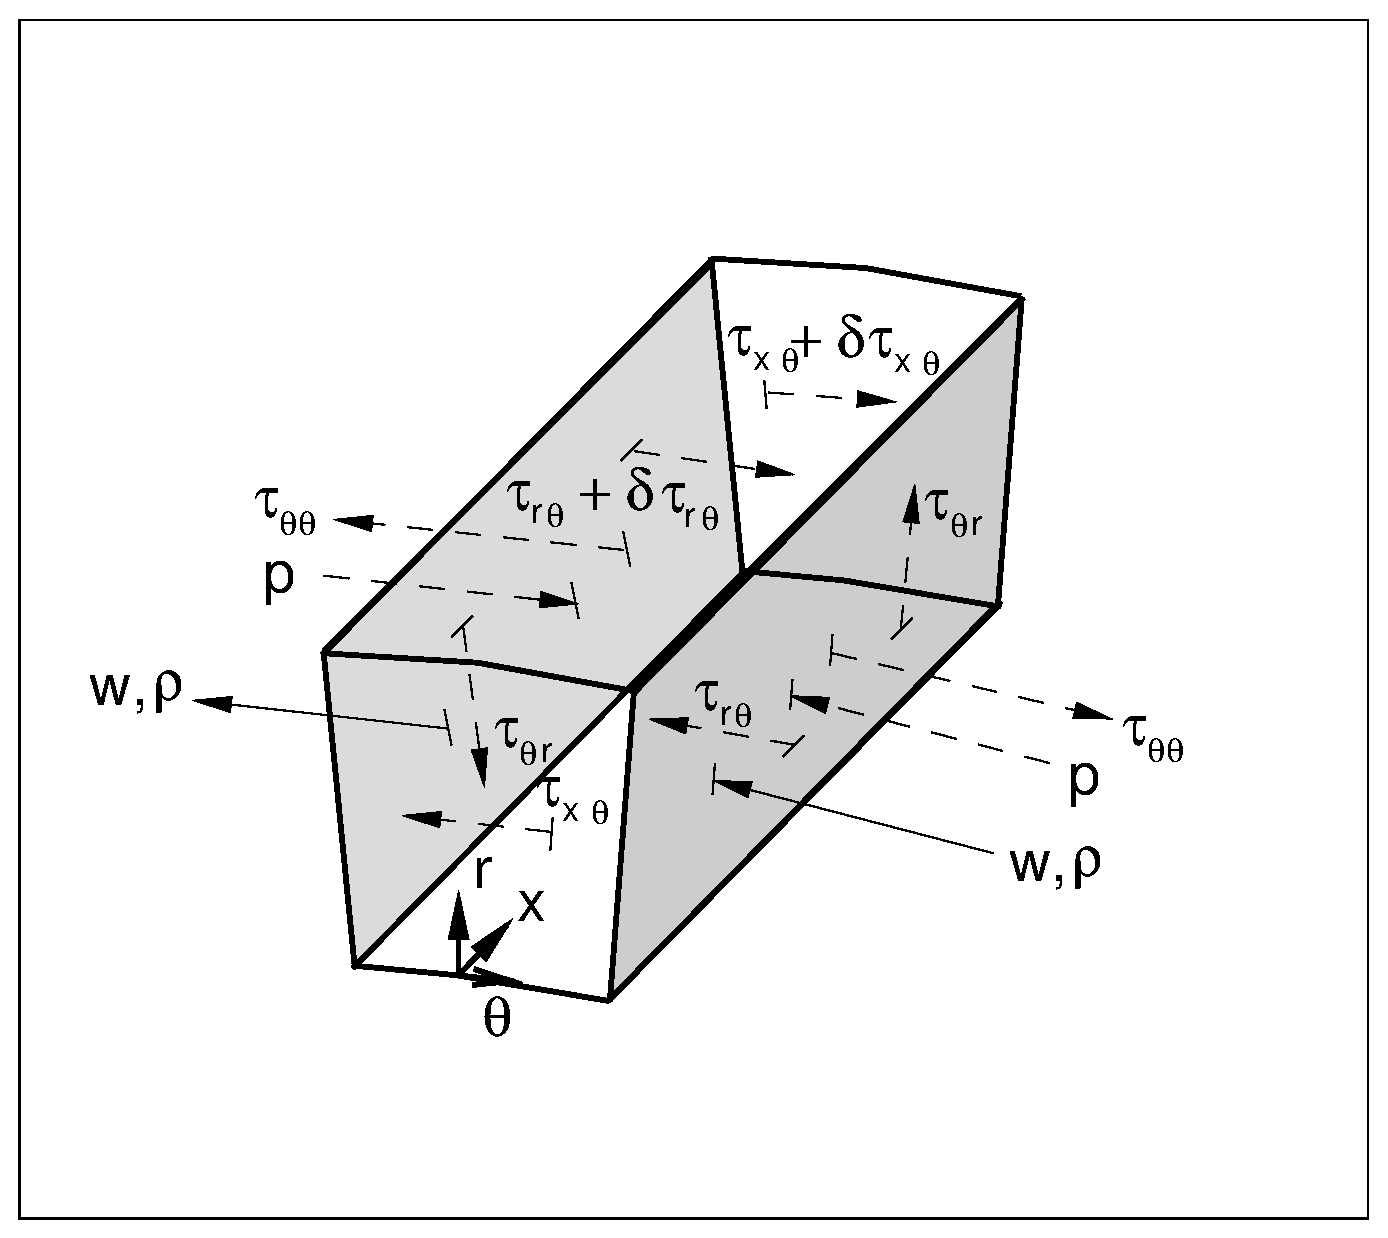
\includegraphics[height=5cm]{./thetadir.eps}
% One can specify [angle=x,width=y,height=z] for the graphics
\caption[$x$ - $r$ planes]{$x$ - $r$ planes : All fluid properties are depicted by solid lines while 
				forces acting on the infantesimal fluid element are depicted by dashed lines (these include
				the pressure acting on the left and right $x$ - $r$ planes
				and the shears acting on all faces of the volume)}
\label{fig:thetadir}
\end{figure}

\begin{displaymath}
	\begin{array}{ccc}
		\textrm{$\theta$ Momentum in through the bottom $x$ - $\theta$ plane} &
		= & (\rho w)(v)dx(R_o \theta)\\
 		& \\ & \\
		\textrm{$\theta$ Momentum out through the top $x$ - $\theta$ plane} &
		= & (\rho w + \frac{\partial \rho w}{\partial r}dr)(v + \frac{\partial v}{\partial r}dr)dx
		(R_o + dr) \theta 
	\end{array}
\end{displaymath}

	Taking the difference between the outflow and inflow $x$ - $\theta$ planes yields (while again neglecting
triple products of differentials and combining terms),

\begin{displaymath}
	\begin{array}{c}
	\Delta \theta_{momentum_{x \theta}}=
		\begin{array}{c}
	(\rho vw + \rho w \frac{\partial v}{\partial r}dr + 
	v \frac{\partial \rho w}{\partial r}dr + \frac{\partial v}{\partial r} \frac{\partial \rho w}{\partial r}dr^2 -
	\rho vw)dx(R_o \theta) \\
	 + (\rho vw + \rho w \frac{\partial v}{\partial r}dr + v \frac{\partial \rho w}{\partial r}dr + 
	\frac{\partial v}{\partial r} \frac{\partial \rho w}{\partial r}dr^2)dxdr \theta
		\end{array} \\ \\
	\Delta \theta_{momentum_{x \theta}}= (\frac{\partial \rho vw}{\partial r})dxdr (R_o \theta) + (\rho vw)dxdr \theta
	\end{array}
\end{displaymath}

\begin{displaymath}
	\begin{array}{ccc}
		\textrm{$\theta$ Momentum in through the front $r$ - $\theta$ plane} &
		= & (\rho w)(u)dr(R_o \theta)\\
 		& \\ & \\
		\textrm{$\theta$ Momentum out through the back $r$ - $\theta$ plane} &
		= & (\rho w + \frac{\partial \rho w}{\partial x}dx)(u + \frac{\partial u}{\partial x}dx)dr(R_o \theta) 
	\end{array}
\end{displaymath}

	Taking the difference between the outflow and inflow $r$ - $\theta$ planes yields,

\begin{displaymath}
	\begin{array}{c}
	\Delta \theta_{momentum_{r \theta}}=(\rho uw + \rho w \frac{\partial u}{\partial x}dx + 
	u \frac{\partial \rho w}{\partial x}dx +
	 \frac{\partial u}{\partial x} \frac{\partial\rho w}{\partial x}dx^2 - \rho uw)dr(R_o \theta) \\ \\
	\Delta \theta_{momentum_{r \theta}}=(\frac{\partial \rho uw}{\partial x})dxdr(R_o \theta)
	\end{array}
\end{displaymath}

	Allowing for an unsteady change in the $\theta$ direction momentum and applying Newton's second law

\begin{displaymath}
	\frac{\partial \rho w}{\partial t}dxdr(R_o \theta) + \Delta \theta_{momentum_{r \theta}} + \Delta \theta_{momentum_{x \theta}} = 
	\sum \textrm{Forces}_\theta
\end{displaymath}

	which after making the appropriate substitutions yields

\begin{displaymath}
	\Big\{(\frac{\partial \rho w}{\partial t} + \frac{\partial \rho uw}{\partial x} +
	\frac{\partial \rho vw}{\partial r})(R_o \theta) + (\rho vw \theta)\Big\}dxdr = \sum \textrm{Forces}_\theta
\end{displaymath}

	However, $\theta$ can be eliminated through the use of Eq.\ref{eqn:theta} to obtain

\begin{equation}
	\Big\{\frac{\partial \rho w}{\partial t} + \frac{\partial \rho uw}{\partial x} +
	\frac{\partial \rho vw}{\partial r} + \frac{1}{r}(\rho vw)\Big\}dxdr = \sum \textrm{Forces}_\theta
\label{eqn:thetamomchg}
\end{equation}

	Examining each of the forces contributing to an overall force in the $\theta$ direction individually, one 
can complete the right hand side of Eq.\ref{eqn:thetamomchg}.  As for the $r$ direction derivations, the distance
between the centre of the infantesimal volume and the boundaries will be considered to be $\frac{\theta}{2}$.
As well, the definition of two additional stress terms is required for the purposes of this derivation.  However, 
since the $\theta$ momentum equation is only a stepping stone used in deriving the turbulent set of axisymmetric 
equations, they are included here for completeness only.

\begin{displaymath}
	\begin{array}{ccc}
		\begin{array}{c}
		\textrm{Force exerted on the left $x$ - $r$ plane} \\
		\textrm{by the pressure and shears (normal and parallel)} \\
		\textrm{on its surface in the $\theta$ direction}
		\end{array} 
		& = &
		\begin{array}{c}
		(-p \cos{\frac{\theta}{2}} + \tau_{\theta \theta}\cos{\frac{\theta}{2}} \\
		-\tau_{\theta r}\sin{\frac{\theta}{2}}) dxdr
		\end{array} \\
	& \\ & \\
		\begin{array}{c}
		\textrm{Force exerted on the right $x$ - $r$ plane}\\
		\textrm{by the pressure and shears (normal and parallel)} \\
		\textrm{on its surface in the $\theta$ direction}
		\end{array} 
		& = &
		\begin{array}{c}
		(p \cos{\frac{\theta}{2}} - \tau_{\theta \theta}\cos{\frac{\theta}{2}} \\
		-\tau_{\theta r}\sin{\frac{\theta}{2}}) dxdr	
		\end{array}
	\end{array} 
\end{displaymath}
\\
\begin{displaymath}
	\begin{array}{ccc}
		\begin{array}{c}
		\textrm{Force exerted on the bottom $x$- $\theta$ plane} \\
		\textrm{by the shear on its surface}
		\end{array} & = &
		-\tau_{r\theta}dx (R_o \theta) \\
   	& \\ & \\
		\begin{array}{c}
		\textrm{Force exerted on the top $x$ - $\theta$ plane}\\
		\textrm{by the shear on its surface}
		\end{array} & = &
		(\tau_{r\theta} + \frac{\partial \tau_{r\theta}}{\partial r}dr) dx (R_o + dr) \theta
	\end{array}
\end{displaymath}

\begin{displaymath}
	\begin{array}{ccc}
		\begin{array}{c}
		\textrm{Force exerted on the front $r$- $\theta$ plane} \\
		\textrm{by the shear on its surface}
		\end{array} & = &
		-\tau_{x\theta}dr (R_o \theta) \\
   	& \\ & \\
		\begin{array}{c}
		\textrm{Force exerted on the back $r$ - $\theta$ plane}\\
		\textrm{by the shear on its surface}
		\end{array} & = &
		(\tau_{x\theta} + \frac{\partial \tau_{x\theta}}{\partial x}dx) dr (R_o \theta) 
	\end{array}
\end{displaymath}

	Summing all the forces considered, the total force in the $\theta$ - direction becomes,

\begin{displaymath}
	\begin{array}{ccc}
	\sum \textrm{Forces}_\theta & = &
		\begin{array}{c}
			(-p \cos{\frac{\theta}{2}} + p \cos{\frac{\theta}{2}} 
			 + \tau_{\theta \theta}\cos{\frac{\theta}{2}} - \tau_{\theta \theta}\cos{\frac{\theta}{2}}
			-\tau_{\theta r}\sin{\frac{\theta}{2}} -\tau_{\theta r}\sin{\frac{\theta}{2}})dxdr \\
			+ (-\tau_{r\theta}dx + \tau_{r\theta}dx + \frac{\partial \tau_{r\theta}}{\partial r}dxdr
			- \tau_{x\theta}dr + \tau_{x\theta}dr + \frac{\partial \tau_{x\theta}}{\partial x}dxdr)(R_o \theta) \\
			+(\tau_{r\theta} + \frac{\partial \tau_{r\theta}}{\partial r}dr)dxdr \theta
		\end{array}
	\end{array}
\end{displaymath}

	which after canceling like terms, inserting Eqs. \ref{eqn:smallangle} and \ref{eqn:theta} while neglecting 
triple products of differentials (and noting $\tau_{\theta r} = \tau_{r \theta}$) reduces to

\begin{equation}
	\begin{array}{ccc}
	\sum \textrm{Forces}_\theta & = &
		\Big\{\frac{\partial \tau_{x\theta}}{\partial x}
		+ \frac{\partial \tau_{r\theta}}{\partial r} + \frac{1}{r}(2\tau_{r \theta})\Big\}dxdr
	\end{array}
\label{eqn:thetaforces}
\end{equation}

	Therefore combining Eqs. \ref{eqn:thetamomchg} and \ref{eqn:thetaforces} yields the desired form of the 
$\theta$ momentum equation,

\begin{equation}
\frac{\partial}{\partial t}(\rho w) + \frac{\partial}{\partial x}(\rho uw) +
\frac{\partial}{\partial r}(\rho vw) + \frac{1}{r}(\rho vw) = 
\frac{\partial}{\partial x}(\tau_{x\theta}) + \frac{\partial}{\partial r}(\tau_{r\theta}) + 
\frac{1}{r}(2\tau_{r\theta})
\label{eqn:thetamom}
\end{equation}

\subsubsection{Definition of Shear Stresses Normal to the $\theta$ - Direction}
 
\begin{displaymath}
	\tau_{x\theta} = \tau_{\theta x} = \mu(\frac{\partial w}{\partial x} + \frac{1}{r}\frac{\partial u}{\partial \theta})
\end{displaymath}
\begin{displaymath}
	\tau_{r\theta} = \tau_{\theta r} = \mu(\frac{1}{r}\frac{\partial v}{\partial \theta} + r\frac{\partial}{\partial r}
	\frac{w}{r})
\end{displaymath}

	where when combined with the axisymmetric assumption of Eq. \ref{eqn:dtheta} both of these quantities can be
reduced to

\begin{equation}
	\tau_{x\theta} = \tau_{\theta x} = \mu\frac{\partial w}{\partial x}	
\label{eqn:tauxtheta}
\end{equation}

\begin{equation}
	\tau_{r\theta} = \tau_{\theta r} = \mu r\frac{\partial}{\partial r}\frac{w}{r} = 
	\mu \frac{\partial w}{\partial r} - \frac{\mu}{r}w	
\label{eqn:taurtheta}
\end{equation}

%----------------------------------------------------------------------------------------------------------------------
\subsection{Circumferential Additions to the Axisymmetric Energy Equation}

	The axisymmetric energy equation as derived previously (see Eq. \ref{eqn:energyshear}) is repeated below
(without the turbulence terms as these will derived presently),

\begin{equation}
	\begin{array}{ccc}
		\begin{array}{c}
		\Big\{\frac{\partial}{\partial t}(\rho E) +\frac{\partial}{\partial x}(\rho E u + pu) \\
		+ \frac{\partial}{\partial r}(\rho E v + pv) + \frac{1}{r}(\rho E v + pv)\Big\}
		\end{array} & = &
		\begin{array}{c}
			\frac{\partial}{\partial x}\Big\{
			\sum_k (\nu_k \frac{\partial c_k}{\partial x}h_k) 
			- q_{c_x} +  \tau_{xx}u + \tau_{xr}v \Big\} \\
			\frac{\partial}{\partial r}\Big\{
			\sum_k (\nu_k \frac{\partial c_k}{\partial r}h_k)
			-  q_{c_r} + \tau_{rx}u + \tau_{rr}v  \Big\} \\
			+\frac{1}{r}\Big\{\sum_k (\nu_k \frac{\partial c_k}{\partial r}h_k) - q_{c_r} + \tau_{rx}u 
			+ \tau_{rr}v\Big\}
		\end{array}  
	\end{array}
\label{eqn:energy2}
\end{equation}

	Any additions to this equation are going to be added to one of the four main components that comprise the
overall energy equation, (i) the rate of change of total energy, (ii) energy transfer due to species diffusion,
(iii) energy transfer due to heat, (iv) rate of work done.  Starting with the first component, since the 
axisymmetric assumption of Eq. \ref{eqn:dtheta} negates any change of properties in the circumferential 
direction, this requires that the total energy entering and exiting the infantesimal volume through the 
left and right $x$ - $r$ planes be equal.  Therefore there is no addition to this component of the energy
equation.  However, one must be careful in the definition of E, the specific energy, as it was defined as the 
sum of the specific internal and kinetic energies (Eq. \ref{eqn:spenergy})

\begin{displaymath}
	E = e + \frac{1}{2}\vec{V}^2 
\end{displaymath}

	Now since the assumption of zero circumferential velocity is not being applied at this point in the derivation, 
the velocity vector must be understood as the vector sum of all \emph{three} co-ordinate direction velocities,

\begin{equation}
	\vec{V}^2 = (u^2 + v^2 + w^2)
\label{eqn:totvel}
\end{equation}

	Considering next the second and third components of the energy equation, since these both rely on 
gradients in concentration and temperature respectively, they too produce no circumferential additions due to the 
assumption of axisymmetric flow.  This leaves only the fourth component, the rate of work done on the infantesimal
volume, to be considered.  In this case, if $w$ is not assumed to be equal to zero, then there is indeed an
addition that must be made to the overall energy equation.  Considering the forces acting in the circumferential
direction as shown in Fig. \ref{fig:thetadir}

\begin{displaymath}
	\begin{array}{ccc}
	   \begin{array}{c}
		\textrm{Work due to pressure acting} \\ \textrm{on the right $x$ - $r$ plane}
	   \end{array} & = &
	(-p\cos{\frac{\theta}{2}})w dxdr
	\\ & & \\
	   \begin{array}{c}
		\textrm{Work due to pressure acting} \\ \textrm{on the left $x$ - $r$ plane}
	   \end{array} & = &
	(+p\cos{\frac{\theta}{2}})w dxdr
	\\ & & \\
	   \begin{array}{c}
		\textrm{Work due to normal shear acting} \\ \textrm{on the right $x$ - $r$ plane}
	   \end{array} & = &
	(\tau_{\theta \theta}\cos{\frac{\theta}{2}})w dxdr
	\\ & & \\
	   \begin{array}{c}
		\textrm{Work due to normal shear acting} \\ \textrm{on the left $x$ - $r$ plane}
	   \end{array} & = &
	-(\tau_{\theta \theta}\cos{\frac{\theta}{2}})w dxdr
	\end{array}
\end{displaymath}

	As can be seen, these work terms cancel by inspection.  However, the remaining stress terms must
be accounted for as follows,

\begin{displaymath}
       \begin{array}{ccc}
	\begin{array}{c}
		\textrm{Work due to shear acting} \\ \textrm{on the bottom $x$ - $\theta$ plane}
	\end{array} & = &
	-(\tau_{r\theta}w)dx(R_o \theta)
	\\ & & \\
	\begin{array}{c}
		\textrm{Work due to shear acting} \\ \textrm{on the top $x$ - $\theta$ plane}
	\end{array} & = &
	(\tau_{r \theta} + \frac{\partial \tau_{r \theta}}{\partial r}dr)(w + \frac{\partial w}{\partial r}dr)
	dx(R_o + dr) \theta
	\\ & & \\
	\begin{array}{c}
		\textrm{Work due to shear acting} \\ \textrm{on the front $r$ - $\theta$ plane}
	\end{array} & = &
	-(\tau_{x \theta}w)dr(R_o \theta)
	\\ & & \\
	\begin{array}{c}
		\textrm{Work due to shear acting} \\ \textrm{on the back $r$ - $\theta$ plane}
	\end{array} & = &
	(\tau_{x \theta} + \frac{\partial \tau_{x \theta}}{\partial x}dx)(w + \frac{\partial w}{\partial x}dx)
	dr (R_o \theta)
       \end{array}
\end{displaymath}

	Summing the above terms yields,

\begin{displaymath}
	\begin{array}{ccc}
		\Delta \dot{W}_\theta & = &
		\begin{array}{c}
		(-\tau_{r \theta}w dx  + \tau_{r \theta}w dx + w\frac{\partial \tau_{r \theta}}{\partial r}dxdr
		+\tau_{r \theta}\frac{\partial w}{\partial r}dxdr + \frac{\partial \tau_{r \theta}}{\partial r}
		\frac{\partial w}{\partial r}dxdr^2 \\
		-\tau_{x \theta}w dr + \tau_{x \theta} w dr + w\frac{\partial \tau_{x \theta}}{\partial x}dxdr
		+\tau_{x \theta}\frac{\partial w}{\partial x}dxdr + \frac{\partial \tau_{x \theta}}{\partial x}
		\frac{\partial w}{\partial x}dx^2dr)(R_o \theta) \\
		+(\tau_{r \theta}w + w\frac{\partial \tau_{r \theta}}{\partial r}dr
		+\tau_{r \theta}\frac{\partial w}{\partial r}dr + \frac{\partial \tau_{r \theta}}{\partial r}
		\frac{\partial w}{\partial r}dr^2)(dxdr\theta)
		\end{array}
	\end{array}
\end{displaymath}

	Using the result expressed in Eq. \ref{eqn:theta}, combining derivatives and neglecting terms with triple 
products of differentials (and higher) yields

\begin{displaymath}
	\begin{array}{ccc}
		\Delta \dot{W}_\theta & = & \Big\{
		\frac{\partial \tau_{x \theta}w}{\partial x} + \frac{\partial \tau_{r \theta}w}{\partial r}
		+ \frac{1}{r}(\tau_{r \theta}w)\Big\}dxdr
	\end{array}
\end{displaymath}

	It is noted again that the remaining shears acting parallel to the left and right $x$ - $r$ planes
produce no contribution to the work terms as they act perpendicular to the circumferential velocity (see 
Eq. \ref{eqn:workdotproduct}).

	Therefore including the possibility of a non-zero value for the circumferential velocity in the 
energy equation by combining $\Delta \dot{W}_\theta$ with Eq. \ref{eqn:energy2} yields,

\begin{equation}
	\begin{array}{ccc}
		\begin{array}{c}
		\Big\{\frac{\partial}{\partial t}(\rho E) +\frac{\partial}{\partial x}(\rho E u + pu) \\
		+ \frac{\partial}{\partial r}(\rho E v + pv) + \frac{1}{r}(\rho E v + pv)\Big\}
		\end{array} & = &
		\begin{array}{c}
			\frac{\partial}{\partial x}\Big\{
			\sum_k (\nu_k \frac{\partial c_k}{\partial x}h_k) 
			- q_{c_x} +  \tau_{xx}u + \tau_{xr}v + \tau_{x\theta}w\Big\} \\
			\frac{\partial}{\partial r}\Big\{
			\sum_k (\nu_k \frac{\partial c_k}{\partial r}h_k)
			-  q_{c_r} + \tau_{rx}u + \tau_{rr}v  + \tau_{r\theta}w\Big\} \\
			\frac{1}{r}\Big\{\sum_k (\nu_k \frac{\partial c_k}{\partial r}h_k) - q_{c_r} + \tau_{rx}u 
			+ \tau_{rr}v + \tau_{r\theta}w\Big\}
		\end{array}  
	\end{array}
\label{eqn:wenergy}
\end{equation}

	Of course, if $w$ is assumed to be zero, then the Eq. \ref{eqn:wenergy} collapses as expected back
to Eq. \ref{eqn:energy2}.

%--------------------------------------------------------------------------------------------------------------
\subsection{Species Conservation}

	Starting with the laminar species conservation equation as previously derived and shown in 
Eq. \ref{eqn:speciesfinal} and rewritten here for convenience,

\begin{equation}
	\frac{\partial}{\partial t}(\rho_k) + \frac{\partial}{\partial x}(\rho_k u) + \frac{\partial}{\partial r}(\rho_k v)
	+ \frac {1}{r}(\rho_k v) = \frac{\partial}{\partial x}(\nu_k \frac{\partial c_k}{\partial x}) + \frac{\partial}
	{\partial r}(\nu_k \frac{\partial c_k}{\partial r}) + \frac {1}{r}(\nu_k \frac{\partial c_k}{\partial r})
\label{eqn:speciesfinal2}
\end{equation}

	we will make use of the relation expressed in Eq. \ref{eqn:conc} to phrase the above equation entirely in 
terms of species concentrations, $c_k$, and then take the Reynolds average of the resulting expression.  However,
as noted earlier, although a Reynolds averag\emph{ing} process is being used, the actual flow properties (concentration
and velocities) being averaged are Favre averag\emph{ed}.

\begin{displaymath}
	\overline{
	\frac{\partial}{\partial t}(\rho c_k) + \frac{\partial}{\partial x}(\rho c_k u) + \frac{\partial}{\partial r}(\rho c_k v)
	+ \frac {1}{r}(\rho c_k v)} = \overline{\frac{\partial}{\partial x}(\nu_k \frac{\partial c_k}{\partial x}) + 
	\frac{\partial}{\partial r}(\nu_k \frac{\partial c_k}{\partial r}) + \frac {1}{r}(\nu_k \frac{\partial c_k}{\partial r})}
\end{displaymath}

	At this point we will need to make use of another property of Reynolds averaging which states that the
Reynolds average of the derivative of a quantity is equal to the derivative of the Reynolds average of that quantity,

\begin{equation}
	\overline{\frac{\partial \phi}{\partial x}} = \frac{\partial \overline{\phi}}{\partial x}
\label{eqn:reyderiv}
\end{equation} 

	Using this result and that expressed in Eq. \ref{eqn:sums} we can consider each term in the modified species
concentration equation individually.  Therefore, starting with the time dependent term,

\begin{displaymath}
	\overline{\frac{\partial}{\partial t}(\rho c_k)} = \frac{\partial}{\partial t}\overline{\rho c_k} = 
	\frac{\partial}{\partial t}\overline{\rho}\tilde c_k
\end{displaymath}

	where Eq. \ref{eqn:rhophi} was used to simplify the double product.  Considering next the spatial derivative
terms (both $u$ and $v$ are treated in the same fashion, thus only one will be shown),

\begin{displaymath}
	\overline{\frac{\partial}{\partial r}(\rho c_k v)} = \frac{\partial}{\partial r}\overline{\rho c_k v} = 
	\frac{\partial}{\partial r}\Big\{(\overline{\rho}\tilde c_k\tilde{v}) + \overline{\rho c_k'' v''}\Big\}
\end{displaymath}

	where Eq. \ref{eqn:tripleprod} is used to simplify the triple product.  Now since the inviscid axisymmetric 
source term is the same as the above with $\frac {1}{r}$ replacing the derivative $\frac{\partial}{\partial r}$,
one arrives at the same result given that the $\frac{1}{r}$ term is constant with respect to the
Reynolds average at a given location and hence is unaffected by the averaging process.  Thus summarizing the 
results of Reynolds averaging the inviscid terms,

\begin{displaymath}
	\frac{\partial}{\partial t}\overline{\rho}\tilde c_k + \frac{\partial}{\partial x}\Big\{
	(\overline{\rho}\tilde c_k\tilde{u}) + \overline{\rho c_k'' u''}\Big\} + \frac{\partial}{\partial r}\Big\{
	(\overline{\rho}\tilde c_k\tilde{v}) + \overline{\rho c_k'' v''}\Big\}	+ \frac{1}{r}\Big\{
	(\overline{\rho}\tilde c_k\tilde{v}) + \overline{\rho c_k'' v''}\Big\} = \textrm{Viscous Terms}
\end{displaymath}

	At this point it is noted that the inviscid axisymmetric turbulent equation has three additional terms when
compared to its laminar counterpart.  These terms are often referred to as \emph{Reynolds stresses} which exist only
for turbulent flow, given that if there exist no fluctuations in the flow properties the double primed quantities are
zero (they are referred to as stresses as their units are $N/m^2$).  Leaving these terms for the moment and considering 
the remaining viscous terms in the species conservation equation (again considering only one spatial dimension as the 
other is treated exactly the same),

\begin{displaymath}
	\overline{\frac{\partial}{\partial r}(\nu_k \frac{\partial c_k}{\partial r})} = 
	\frac{\partial}{\partial r}\Big\{\overline{\nu_k} \overline{\frac{\partial c_k}{\partial r}} +
	\overline{\nu_k' (\frac{\partial c_k}{\partial r})'}\Big\}
\end{displaymath}

	where Eqs. \ref{eqn:product} and \ref{eqn:reyderiv} were applied.  If one further decomposes the concentration 
into its Favre averaged components while making further use of Eqs. \ref{eqn:reyderiv} and \ref{eqn:sums} one can write,

\begin{displaymath}
	\overline{\frac{\partial}{\partial r}(\nu_k \frac{\partial c_k}{\partial r})} = \frac{\partial}{\partial r}\Big\{
	\overline{\nu_k}\frac{\partial}{\partial r}
	\overline{(\tilde c_k + c_k'')} + \overline{\nu_k' (\frac{\partial c_k}{\partial r})'}\Big\} = \frac{\partial}
	{\partial r}\Bigg\{
	\overline{\nu_k}\frac{\partial}{\partial r} \tilde c_k + \Big\{\overline{\nu_k}\frac{\partial}{\partial r}\overline{c_k''} 
	+ \overline{\nu_k' (\frac{\partial c_k}{\partial r})'}\Big\}\Bigg\}
\end{displaymath}

	At this point we make a simplification regarding the terms in the inner curly braces.  It is noted that these
terms represent the effect of the turbulent fluctuating motion on the laminar diffusion terms (as 
these are the terms under consideration).  However, with the knowledge that the diffusion driven by the large scale 
movement of turbulent eddies within the flow field will be orders of magnitude more significant than that driven
by laminar diffusion (i.e. due solely to gradients in concentration) the terms in the inner curly braces will be neglected.
This does not mean one assumes these turbulent fluctuating terms to be zero, but rather that in comparison to the Reynolds
stresses (which are responsible for the large scale movement of turbulent eddies) the effect of the overall laminar
diffusion terms (including those in the inner curly braces) will be neglible.  Thus the turbulent viscous terms will be 
approximated by,

\begin{equation}
	\overline{\frac{\partial}{\partial r}(\nu_k \frac{\partial c_k}{\partial r}}) \approx 
	\frac{\partial}{\partial r}(\overline{\nu_k}\frac{\partial \tilde c_k}{\partial r})
\label{eqn:difffluxapprox}
\end{equation}

	Extending this result to the remaining viscous terms (the $x$ direction derivative and the viscous axisymmetric 
source term) while combining the inviscid results and rearranging yields,

\begin{displaymath}
	\frac{\partial}{\partial t}\overline{\rho}\tilde c_k + \frac{\partial}{\partial x}
	(\overline{\rho}\tilde c_k\tilde{u})  + \frac{\partial}{\partial r}
	(\overline{\rho}\tilde c_k\tilde{v})	+ \frac{1}{r}
	(\overline{\rho}\tilde c_k\tilde{v})  = 
	\begin{array}{c}
		\frac{\partial}{\partial x}\Big\{
		\overline{\nu_k}\frac{\partial \tilde c_k}{\partial x} - \overline{\rho c_k'' u''}\Big\} +
		\frac{\partial}{\partial r} \Big\{\overline{\nu_k}\frac{\partial \tilde c_k}{\partial r} 
		- \overline{\rho c_k'' v''}\Big\} \\
		+ \frac{1}{r}\Big\{\overline{\nu_k}\frac{\partial \tilde c_k}{\partial r} 
		- \overline{\rho c_k'' v''}\Big\}
	\end{array}
\end{displaymath}

	The only task remaining is to develop an expression for calculating the Reynolds stresses.  To do this one
can make use of the Boussinesq approximation, which is an eddy viscosity formulation (i.e., one proposes the existence
of a turbulent eddy viscosity similar in function to the familiar laminar viscosity, with the important difference however
that this eddy viscosity is a property of both the state of the flow and the properties of the fluid itself, as opposed to 
the laminar viscosity which is dependent solely on the state of the fluid) which relates the products of fluctuating 
properties to the gradient in the average value of the property along a given direction,

\begin{equation}
	\overline{\rho \phi'' u''} \approx -\mu_T \frac{\partial \tilde{\phi}}{\partial x}
\label{eqn:boussinesq}
\end{equation}

	where $\mu_T$ is the turbulent eddy viscosity, the derivative is taken with respect to the 
direction of the fluctuating velocity, and $\phi ''$ is the fluctuating property of interest.  Thus using 
Eq. \ref{eqn:boussinesq} one can rewrite the Reynolds stresses as,

\begin{equation}
	\overline{\rho v'' c_k''} = -\frac{\mu_T}{Sc_T}\frac{\partial \tilde c_k}{\partial r}
\label{eqn:turbdiffapprox}
\end{equation}	

	where the Schmidt number is used to relate the turbulent eddy viscosity to the laminar diffusion
co-efficient (see Eq. \ref{eqn:nuk}).  

\begin{equation}
	Sc_T = \frac{\mu_T}{\rho D_{kl}} = \frac{\mu_T}{\nu_k}
\label{eqn:schmidt}
\end{equation} 

	Also note that the above Reynolds stress approximation is exactly the same in the $x$ direction 
but with $x$ replacing $r$.  Therefore one can rewrite the turbulent axisymmetric species continuity equation as,

\begin{displaymath}
	\frac{\partial}{\partial t}\overline{\rho}\tilde c_k + \frac{\partial}{\partial x}
	(\overline{\rho}\tilde c_k\tilde{u})  + \frac{\partial}{\partial r}
	(\overline{\rho}\tilde c_k\tilde{v})	+ \frac{1}{r}
	(\overline{\rho}\tilde c_k\tilde{v}) = 
	\begin{array}{c}
		\frac{\partial}{\partial x}\Big\{(\overline{\nu_k} + \frac{\mu_T}{Sc_T})
		\frac{\partial \tilde c_k}{\partial x}\Big\} +
		\frac{\partial}{\partial r} \Big\{(\overline{\nu_k} + \frac{\mu_T}{Sc_T})
		\frac{\partial \tilde c_k}{\partial r}\Big\} \\
		+ \frac{1}{r}\Big\{(\overline{\nu_k} + \frac{\mu_T}{Sc_T})\frac{\partial \tilde c_k}{\partial r}\Big\}
	\end{array}
\end{displaymath}

	If one further defines a turbulent diffusion co-efficient as,

\begin{equation}
	\nu_k^* = \overline{\nu_k} + \frac{\mu_T}{Sc_T}
\label{eqn:nukstar} 
\end{equation}

	one can write the final version of the turbulent equation as,

\begin{equation}
	\frac{\partial}{\partial t}\overline{\rho}\tilde c_k + \frac{\partial}{\partial x}
	(\overline{\rho}\tilde c_k\tilde{u})  + \frac{\partial}{\partial r}
	(\overline{\rho}\tilde c_k\tilde{v})	+ \frac{1}{r}
	(\overline{\rho}\tilde c_k\tilde{v}) = \frac{\partial}{\partial x}(
	\nu_k^*\frac{\partial \tilde c_k}{\partial x}) +
	\frac{\partial}{\partial r} (\nu_k^*\frac{\partial \tilde c_k}{\partial r})
	+ \frac{1}{r}(\nu_k^*\frac{\partial \tilde c_k}{\partial r})
\label{eqn:turbspeciesfinal}
\end{equation}

	In this form, one can immediately see the benefit of using the Boussinesq approximation as 
when compared with Eq. \ref{eqn:speciesfinal2} (with the substitution made for $\rho_k$),

\begin{displaymath}
	\frac{\partial}{\partial t}(\rho c_k) + \frac{\partial}{\partial x}(\rho c_k u) + \frac{\partial}{\partial r}(\rho c_k v)
	+ \frac {1}{r}(\rho c_k v) = \frac{\partial}{\partial x}(\nu_k \frac{\partial c_k}{\partial x}) + \frac{\partial}
	{\partial r}(\nu_k \frac{\partial c_k}{\partial r}) + \frac {1}{r}(\nu_k \frac{\partial c_k}{\partial r})
\end{displaymath}

	one can see that both the laminar and turbulent equations have exactly the same form.  Thus from the viewpoint
of their solution, the only thing that needs to be modified is the definition of the diffusion co-efficient, using either
Eq. \ref{eqn:nukstar} or Eq. \ref{eqn:nuk} (although it is also noted that in the case of turbulent flow one must remember
that the equation is solving for the Favre averaged value of species concentration).  

	As a final consideration, since the global continuity equation is directly related to the species concentration
equation, it is prudent to develop its turbulent counterpart here as well.  Starting with the laminar axisymmetric 
equation (see Eq. \ref{eqn:globalcont} and taking the Reynolds average
	
\begin{displaymath}
	\overline{\frac{\partial}{\partial t}(\rho) + \frac{\partial}{\partial x}(\rho u) + 
	\frac{\partial}{\partial r}(\rho v) + \frac{1}{r}(\rho v)} = 0 
\end{displaymath}

\begin{equation}
	\frac{\partial}{\partial t}(\overline{\rho}) + \frac{\partial}{\partial x}(\overline{\rho}\tilde{u})
	 + \frac{\partial}{\partial r}(\overline{\rho}\tilde{v}) + \frac{1}{r}(\overline{\rho}\tilde{v}) = 0
\label{eqn:turbglobalcont}
\end{equation}

	where Eqs. \ref{eqn:sums}, \ref{eqn:rhophi}, and \ref{eqn:reyderiv} are used to simplify the above expression.  
It is clearly seen that there is no difference between the laminar and turbulent global continuity equations except for 
the quantities being solved for, as the form of the two equations is identical.

%----------------------------------------------------------------------------------------------------------------------------
\subsection{$x$ Momentum Equation}

	The previously derived laminar $x$ momentum equation without substitution of the stress terms is repeated here
in a slightly rearranged form so that we may derive its turbulent counterpart.

\begin{equation}
\overline{\frac{\partial}{\partial t}(\rho u) + \frac{\partial}{\partial x}(\rho u^2 + p) +
\frac{\partial}{\partial r}(\rho uv) + \frac{1}{r}(\rho u v)} = \overline{ 
\frac{\partial}{\partial x}(\tau_{xx}) + \frac{\partial}{\partial r}(\tau_{rx}) + \frac{1}{r}(\tau_{rx})}
\label{eqn:xmomshear2}
\end{equation}

	Using Eq. \ref{eqn:sums} to break the turbulent equation into individual components and
starting first with the time dependent term, using Eqs. \ref{eqn:reyderiv} and \ref{eqn:rhophi} 
one can write,

\begin{displaymath}
	\overline{\frac{\partial}{\partial t}(\rho u)} = \frac{\partial}{\partial t}(\overline{\rho}\tilde{u})
\end{displaymath}

	Considering next the inviscid $x$ derivative term,

\begin{displaymath}
	\overline{\frac{\partial}{\partial x}(\rho u^2 + p)} = \frac{\partial}{\partial x}(\overline{\rho u u}) + 
	\frac{\partial}{\partial x}(\overline{p}) = \frac{\partial}{\partial x}\Big\{\overline{\rho}\tilde{u}\tilde{u} +
	\overline{\rho u'' u''} + \overline{p}\Big\}
\end{displaymath}

	where Eq. \ref{eqn:tripleprod} was used to evaluate $\overline{\rho u u}$.  Using similar logic for 
the inviscid $r$ derivative term (and hence the inviscid axisymmetric source term as well),

\begin{displaymath}
	\overline{\frac{\partial}{\partial r}(\rho uv)} = \frac{\partial}{\partial r}(\overline{\rho u v}) 
	= \frac{\partial}{\partial r}\Big\{\overline{\rho}\tilde{u}\tilde{v} +
	\overline{\rho u'' v''}\Big\}
\end{displaymath}

\begin{displaymath}
	\overline{\frac{1}{r}(\rho uv)} = \frac{1}{r}(\overline{\rho u v}) 
	= \frac{1}{r}\Big\{\overline{\rho}\tilde{u}\tilde{v} +
	\overline{\rho u'' v''}\Big\}
\end{displaymath}

	Combining the inviscid turbulence results yields,

\begin{equation}
	\frac{\partial}{\partial t}(\overline{\rho}\tilde{u}) + \frac{\partial}{\partial x}\Big\{
	\overline{\rho}\tilde{u}^2 + \overline{p} + \overline{\rho u'' u''}\Big\} + \frac{\partial}{\partial r}\Big\{
	\overline{\rho}\tilde{u}\tilde{v} + \overline{\rho u'' v''}\Big\} + \frac{1}{r}\Big\{
	\overline{\rho}\tilde{u}\tilde{v} + \overline{\rho u'' v''}\Big\} = \textrm{Viscous Terms}
\label{eqn:xmomturbinv}
\end{equation}

	Moving on to the viscous terms, we shall need to make use of the definitions of the various stress terms
defined earlier so that the proper variables can be decomposed into their Favre averaged components.  
Starting with the definition of $\tau _{xx}$ as shown in Eq. \ref{eqn:tauxxlambda}  
and substituting Stokes hypothesis (Eq. \ref{eqn:stokes}) one can write,

\begin{displaymath}
	\overline{\frac{\partial}{\partial x}(\tau_{xx})} = \overline{\frac{\partial}{\partial x}\Big\{
	2\mu \frac{\partial u}{\partial x} - \frac{2}{3}\mu (\nabla \cdot \vec{V})} \Big\}
\end{displaymath}

	Using the by now familiar rules of Reynolds averaging (Eqs. \ref{eqn:sums} and \ref{eqn:reyderiv}) and
decomposing the above terms using Eq. \ref{eqn:product} yields,

\begin{displaymath}
	\overline{\frac{\partial}{\partial x}\Big\{
	2\mu \frac{\partial u}{\partial x} - \frac{2}{3}\mu (\nabla \cdot \vec{V})} \Big\} = \frac{\partial}{\partial x}\Big\{
	2 \overline{\mu} \frac{\partial \overline{u}}{\partial x} + 2\overline{\mu' (\frac{\partial u}{\partial x})'}
	- \frac{2}{3}\overline{\mu} \overline{(\nabla \cdot \vec{V})} - \frac{2}{3}\overline{\mu'(\nabla \cdot \vec{V})'}\Big\}
\end{displaymath}

	At this point one will make use of some foresight combined with the experience gained from deriving
the turbulent version of the species conservation equation.  Since in the species conservation equation each
of the Reynolds stresses arising out of the inviscid flux terms was modeled and then combined with the viscous
term along the matching co-ordinate direction, we assume that this process will also hold true here.  Thus 
we will neglect the Reynolds fluctuating components (') arising from the viscous terms for no other reason than that 
we know they form only a part of the turbulent terms to be added to the $x$ momentum equation.  This does not mean 
that these terms are
assumed to be zero, or even negligible (as was the case in the species conservation equation as the turbulent
diffusion term is known to be magnitudes larger than the laminar counterpart), but rather that these terms are 
capable of being neglected without reducing the resulting equation back down to its laminar origin (as it should
be kept in mind that by taking the Reynolds average of Favre averaged quantities we hope to \emph{add} terms to the 
laminar equation to reflect the existence of turbulence).  However, it is noted that if indeed the Reynolds stresses
are much larger than these terms we are neglecting then this process has a physical justification as well.  
Neglecting these fluctuating terms leaves,

\begin{displaymath}
	\overline{\frac{\partial}{\partial x}\Big\{
	2\mu \frac{\partial u}{\partial x} - \frac{2}{3}\mu (\nabla \cdot \vec{V})} \Big\} = \frac{\partial}{\partial x}\Big\{
	2 \overline{\mu} \frac{\partial \overline{u}}{\partial x} + 
	- \frac{2}{3}\overline{\mu} \overline{(\nabla \cdot \vec{V})} \Big\}
\end{displaymath}

	Examining the second term in more detail using Eq. \ref{eqn:delv},

\begin{displaymath}
	\overline{(\nabla \cdot \vec{V})} = \overline{(\frac{\partial u}{\partial x} +  \frac{\partial v}{\partial r} 
	+ \frac{v}{r} )} = \frac{\partial}{\partial x}\overline{u} + \frac{\partial}{\partial r}\overline{v} +
	\frac{1}{r}\overline{v}
\end{displaymath}
	
	where again the Reynolds averaging rules have been applied.  Decomposing the velocities into their Favre
averaged quantities and their Favre fluctuating components yields,

\begin{displaymath}
	\overline{(\nabla \cdot \vec{V})} = \frac{\partial}{\partial x}\overline{(\tilde{u}+u'')} + 
	\frac{\partial}{\partial r}\overline{(\tilde{v}+v'')} +
	\frac{1}{r}\overline{(\tilde{v}+v'')} = (\frac{\partial \tilde{u}}{\partial x} + \frac{\partial \tilde{v}}
	{\partial r} + \frac{\tilde{v}}{r}) + \Big\{\frac{\partial}{\partial x}\overline{u''} + \frac{\partial}{\partial r}
	\overline{v''} + \frac{1}{r}\overline{v''}\Big\}
\end{displaymath}

	Although it is acknowledged that none of the terms in the curly braces can be assumed to be zero (as shown in 
Eq. \ref{eqn:reyoffavfluc}) we will neglect these terms in order to simplify the Reynolds average of this
term.  Thus with this simplification one can write,

\begin{equation}
	\overline{(\nabla \cdot \vec{V})} \approx (\frac{\partial \tilde{u}}{\partial x} + \frac{\partial \tilde{v}}
	{\partial r} + \frac{\tilde{v}}{r}) 
\label{eqn:delvturb}
\end{equation}

	Going back to the equation for $\tau_{xx}$ and decomposing the $u$ velocity into a Favre average and
Favre fluctuating component,

\begin{displaymath}
	\frac{\partial}{\partial x}\Big\{
	2 \overline{\mu} \frac{\partial \overline{u}}{\partial x} + 
	- \frac{2}{3}\overline{\mu} \overline{(\nabla \cdot \vec{V})} \Big\} = \frac{\partial}{\partial x}\Big\{
	2 \overline{\mu} \frac{\partial}{\partial x}\overline{(\tilde{u}+u'')} + 
	\frac{2}{3}\overline{\mu} \overline{(\nabla \cdot \vec{V})} \Big\} = \frac{\partial}{\partial x}\Big\{
	2\overline{\mu}\frac{\partial \tilde{u}}{\partial x} - \frac{2}{3}\overline{\mu} \overline{(\nabla \cdot \vec{V})}
	+2\overline{\mu}\frac{\partial}{\partial x}\overline{u''}\Big\}
\end{displaymath}

	As was done for the $(\nabla \cdot \vec{V})$ term we will neglect the last term above despite the fact that
it has been proved that the Reynolds average of a Favre fluctuating component is not zero (Eq. \ref{eqn:reyoffavfluc}).
Therefore using the result expressed above and in Eq. \ref{eqn:delvturb}, $\tau_{xx}$ can be approximated by

\begin{equation}
	\overline{\frac{\partial}{\partial x}(\tau_{xx})} \approx \frac{\partial}{\partial x}\Big\{
	2\overline{\mu}\frac{\partial \tilde{u}}{\partial x} - \frac{2}{3}\overline{\mu} (\frac{\partial \tilde{u}}
	{\partial x} + \frac{\partial \tilde{v}}{\partial r} + \frac{\tilde{v}}{r}) 
	\Big\}
\label{eqn:tauxxturb}
\end{equation}

	Using the definition of $\tau_{rx}$ (Eq. \ref{eqn:taurx}) and taking the Reynolds average (using Eqs. \ref{eqn:product}
and \ref{eqn:reyderiv} yields),

\begin{displaymath}
	\overline{\frac{\partial}{\partial r}(\tau_{rx})} = \frac{\partial}{\partial r}\Big\{
	\overline{\mu(\frac{\partial v}{\partial x} + \frac{\partial u}{\partial r})}\Big\} = \frac{\partial}{\partial r}\Big\{
	\overline{\mu}(\overline{\frac{\partial v}{\partial x} + \frac{\partial u}{\partial r}}) + 
	\overline{\mu'(\frac{\partial v}{\partial x} + \frac{\partial u}{\partial r})'}\Big\}
\end{displaymath}

	Here again we note that there will be a Reynolds stress to be combined with this term and hence 
we will neglect the fluctuating components.  Decomposing the
velocities into their Favre averages and Favre fluctuating components while applying Eqs. \ref{eqn:sums} and 
\ref{eqn:reyderiv} yields,

\begin{displaymath}
	\frac{\partial}{\partial r}\Big\{\overline{\mu(\frac{\partial v}{\partial x} + \frac{\partial u}{\partial r})}\Big\} 
	= \frac{\partial}{\partial r}\Big\{\overline{\mu}[\frac{\partial}{\partial x}\overline{(\tilde{v} + v'')} + 
	\frac{\partial}{\partial r}\overline{(\tilde{u} + u'')}]\Big\} =  \frac{\partial}{\partial r}\Big\{\overline{\mu}
	(\frac{\partial \tilde{v}}{\partial x} + \frac{\partial \tilde{u}}{\partial r}) + \overline{\mu}
	(\frac{\partial}{\partial x}\overline{v''} + \frac{\partial}{\partial r}\overline{u''})\Big\}
\end{displaymath}

	As was done for $\tau_{xx}$ and $(\nabla \cdot \vec{V})$, we will again neglect these fluctuating components 
despite the results of Eq. \ref{eqn:reyoffavfluc} thus yielding,

\begin{equation}
	\overline{\frac{\partial}{\partial r}(\tau_{rx})} \approx \frac{\partial}{\partial r}\Big\{\overline{\mu}
	(\frac{\partial \tilde{v}}{\partial x} + \frac{\partial \tilde{u}}{\partial r})\Big\}	
\label{eqn:taurxturb}
\end{equation}

	Given the similarity between the viscous axisymmetric source term and the term derived above, the
same logic can be applied to yield,

\begin{displaymath}
	\overline{\frac{1}{r}(\tau_{rx})} \approx \frac{1}{r}\Big\{\overline{\mu}
	(\frac{\partial \tilde{v}}{\partial x} + \frac{\partial \tilde{u}}{\partial r})\Big\}	
\end{displaymath}

	Thus combining this last result with those obtained in Eqs. \ref{eqn:xmomturbinv}, \ref{eqn:tauxxturb},
and \ref{eqn:taurxturb} and rearranging yields,

\begin{displaymath}
	\begin{array}{ccc}
	\frac{\partial}{\partial t}(\overline{\rho}\tilde{u}) + \frac{\partial}{\partial x}(
	\overline{\rho}\tilde{u}^2 + \overline{p}) + \frac{\partial}{\partial r}(
	\overline{\rho}\tilde{u}\tilde{v}) + \frac{1}{r}(\overline{\rho}\tilde{u}\tilde{v}) 
	& = & 
		\begin{array}{c} 
	\frac{\partial}{\partial x}\Big\{
	2\overline{\mu}\frac{\partial \tilde{u}}{\partial x} - \frac{2}{3}\overline{\mu} (\frac{\partial \tilde{u}}
	{\partial x} + \frac{\partial \tilde{v}}{\partial r} + \frac{\tilde{v}}{r}) - \overline{(\rho u'' u'')} \Big\}
	\\ + \frac{\partial}{\partial r}\Big\{\overline{\mu} 
	(\frac{\partial \tilde{v}}{\partial x} + \frac{\partial \tilde{u}}{\partial r}) - \overline{(\rho u'' v'')}\Big\}\\
	+ \frac{1}{r}\Big\{\overline{\mu}
	(\frac{\partial \tilde{v}}{\partial x} + \frac{\partial \tilde{u}}{\partial r}) - \overline{(\rho u'' v'')}\Big\}	
		\end{array}
	\end{array}
\end{displaymath}

	Using the Boussinesq approach tailored to the fact that we would like each of the Reynolds stresses to be
combined with their viscous counterparts, we will model each of the Reynolds stresses as the product of a turbulent
eddy viscosity and term composed of the same derivatives as found in the matching viscous stress terms.  Thus for
$(\rho u'' u'')$ we will write,

\begin{equation}
	-\overline{(\rho u'' u'')} \approx \mu_T\Big\{2\frac{\partial \tilde{u}}{\partial x} - \frac{2}{3}
	(\frac{\partial \tilde{u}}{\partial x} + \frac{\partial \tilde{v}}{\partial r} + \frac{\tilde{v}}{r})\Big\}
	-\frac{2}{3}\overline{\rho}k
\label{eqn:rhouu}
\end{equation}

	It should be noted that a new term, $\rho k $, has been introduced here which is to be understood as the kinetic
energy of turbulence.  This is a three dimensional quantity composed of the fluctuating components of velocity and
can be expressed as (using Favre fluctuating components),

\begin{equation}
	\overline{\rho} k = \frac {1}{2}(\overline{\rho u'' u''} + \overline{\rho v'' v''} + \overline{\rho w'' w''}) =
	\frac{1}{2}\sum_{i=0}^{i=2}\overline{\rho v_i'' v_i''}
\label{eqn:rhok}
\end{equation} 

	One must be careful not to confuse $w''$ with $\tilde{w}$ in the sense that even if one makes the assumption
that the average circumferential velocity is zero (i.e. $\tilde{w}=0$), this does not necessarily require that the 
fluctuating value of this velocity be zero as well.  Hence for the axisymmetric equations in which there is no
$\theta$ momentum equation used (as is the case for $\tilde{w}=0$) one must still understand the definition of 
$\overline{\rho} k$ to include $w''$.  This point will become clearer after all the Reynolds stresses are modeled, 
where for the approximations to be self consistent the kinetic energy of turbulence must include the fluctuating 
circumferential velocity.

	As for the remaining $(\rho u'' v'')$Reynolds stress we will write,

\begin{equation}
	-\overline{(\rho u'' v'')} \approx \mu_T(\frac{\partial \tilde{v}}{\partial x} + \frac{\partial \tilde{u}}{\partial r})
\label{eqn:rhouv}
\end{equation}

	Thus substituting the approximations made in Eqs. \ref{eqn:rhouu} and \ref{eqn:rhouv} into the $x$ momentum 
equation yields,

\begin{displaymath}
	\begin{array}{ccc}
	\frac{\partial}{\partial t}(\overline{\rho}\tilde{u}) + \frac{\partial}{\partial x}(
	\overline{\rho}\tilde{u}^2 + \overline{p}) + \frac{\partial}{\partial r}(
	\overline{\rho}\tilde{u}\tilde{v}) + \frac{1}{r}(\overline{\rho}\tilde{u}\tilde{v})
	& = & 
		\begin{array}{c} 
	\frac{\partial}{\partial x}\Bigg\{(\overline{\mu}+\mu_T)
	\Big\{2\frac{\partial \tilde{u}}{\partial x} - \frac{2}{3}(\frac{\partial \tilde{u}}
	{\partial x} + \frac{\partial \tilde{v}}{\partial r} + \frac{\tilde{v}}{r})\Big\} -\frac{2}{3}\overline{\rho}k \Bigg\}
	\\ 
	+ \frac{\partial}{\partial r}\Big\{(\overline{\mu} + \mu_T) 
	(\frac{\partial \tilde{v}}{\partial x} + \frac{\partial \tilde{u}}{\partial r})\Big\}\\
	+ \frac{1}{r}\Big\{(\overline{\mu} + \mu_T)
	(\frac{\partial \tilde{v}}{\partial x} + \frac{\partial \tilde{u}}{\partial r})\Big\}	
		\end{array}
	\end{array}
\end{displaymath}

	Defining a total turbulent co-efficient of viscosity as,

\begin{equation}
	\mu^* = \overline{\mu} + \mu_T
\label{eqn:mustar}
\end{equation}

	one can write the turbulent axisymmetric $x$ momentum equation as,

\begin{equation}	
	\frac{\partial}{\partial t}(\rho \tilde{u}) + \frac{\partial}{\partial x}(\rho \tilde{u}^2 + 
	[\overline{p}+\frac{2}{3}\overline{\rho}k]) +
	\frac{\partial}{\partial r}(\rho \tilde{u}\tilde{v}) + \frac{1}{r}(\rho \tilde{u} \tilde{v}) =  
	\frac{\partial}{\partial x}(\tilde{\tau}_{xx}) + \frac{\partial}{\partial r}(\tilde{\tau}_{rx}) 
	+ \frac{1}{r}(\tilde{\tau}_{rx})
\label{eqn:xmomfinalturb}
\end{equation}

	where the definitions of the stresses remain unchanged but with $\mu$ replaced by $\mu^*$ and the
velocities replaced by their Favre averages.  Note that as with the species equation, the turbulent version
of the axisymmetric $x$ momentum equation has the exact same form as its laminar counterpart

\begin{displaymath}
	\frac{\partial}{\partial t}(\rho u) + \frac{\partial}{\partial x}(\rho u^2 + p) +
	\frac{\partial}{\partial r}(\rho uv) + \frac{1}{r}(\rho u v) = 
	\frac{\partial}{\partial x}(\tau_{xx}) + \frac{\partial}{\partial r}(\tau_{rx}) + \frac{1}{r}(\tau_{rx})
\end{displaymath}

but for the use of Favre averaged quantities, a turbulent co-efficient of viscosity and an additional turbulent
pressure component.

%-------------------------------------------------------------------------------------------------------------------------
\subsection{$r$ Momentum Equation}

	Repeating the process used to derive the turbulent $x$ momentum equation, we will start with the laminar
version of the $r$ momentum equation and take the Reynolds average of each term individually,

\begin{equation}
	\overline{\frac{\partial}{\partial t}(\rho v) + \frac{\partial}{\partial x}(\rho uv) +
	\frac{\partial}{\partial r}(\rho v^2 + p) + \frac{1}{r}(\rho v^2)} = 
	\overline{\frac{\partial}{\partial x}(\tau_{xr})
	+ \frac{\partial}{\partial r}(\tau_{rr}) + \frac{1}{r}(\tau_{rr} - \tau_{\theta \theta})}
\label{eqn:rmomshear2}
\end{equation}

	The time dependent term ($\rho v$) and the $x$ derivative term ($\rho u v$) have already been
considered in doing the $x$ momentum equations (but for the fact that the derivative of $\rho u v$ was taken
with respect to $r$ in the previous case and with respect to $x$ in the present case, and instead of $\rho u$
in the time dependent term one has $\rho v$) and so only the results will be repeated here,

\begin{displaymath}
	\overline{\frac{\partial}{\partial t}(\rho v)} = \frac{\partial}{\partial t}(\overline{\rho}\tilde{v})
\end{displaymath}

\begin{displaymath}
	\overline{\frac{\partial}{\partial x}(\rho uv)} = \frac{\partial}{\partial x}\Big\{\overline{\rho}\tilde{u}\tilde{v} +
	\overline{\rho u'' v''}\Big\}
\end{displaymath}

	Likewise, the $r$ derivative term has the same form as the $x$ derivative term of the $x$ momentum equation
but for the use of $v$ in place of $u$, thus the same logic can be applied to obtain the result,

\begin{displaymath}
	\overline{\frac{\partial}{\partial r}(\rho v^2 + p)} = \frac{\partial}{\partial r}\Big\{
	\overline{\rho}\tilde{v}\tilde{v} + \overline{\rho v'' v''} + \overline{p}\Big\}
\end{displaymath}

	Noting that the inviscid axisymmetric source term is identical to the $r$ derivative term minus the 
pressure one can extend the above result to yield,

\begin{displaymath}
	\overline{\frac{1}{r}(\rho v^2)} = \frac{1}{r}\Big\{
	\overline{\rho}\tilde{v}\tilde{v} + \overline{\rho v'' v''}\Big\}
\end{displaymath}

	Thus combining the inviscid results,

\begin{equation}
	\frac{\partial}{\partial t}(\overline{\rho}\tilde{v}) + \frac{\partial}{\partial x}\Big\{
	\overline{\rho}\tilde{u}\tilde{v} + \overline{\rho u'' v''}\Big\} + \frac{\partial}{\partial r}\Big\{
	\overline{\rho}\tilde{v}^2 + \overline{p} + \overline{\rho v'' v''}\Big\} + \frac{1}{r}\Big\{
	\overline{\rho}\tilde{v}^2 + \overline{\rho v'' v''}\Big\} = \textrm{Viscous Terms}
\label{eqn:rmomturbinv}
\end{equation}

	Considering next the viscous terms, we note that since $\tau_{xr} = \tau_{rx}$ we can use the 
results from the $x$ momentum equation on $\tau_{rx}$ (noting that here the derivative is taken with 
respect to $x$ and not $r$).  Therefore,

\begin{displaymath}
	\overline{\frac{\partial}{\partial x}(\tau_{xr})} \approx \frac{\partial}{\partial x}\Big\{\overline{\mu}
	(\frac{\partial \tilde{v}}{\partial x} + \frac{\partial \tilde{u}}{\partial r})\Big\}	
\end{displaymath}

	From the definition of $\tau_{rr}$ shown in Eq. \ref{eqn:taurrlambda},
we note that it has exactly the same form as $\tau_{xx}$ and hence we will extend those results yielding,

\begin{equation}
	\overline{\frac{\partial}{\partial r}(\tau_{rr})} = \overline{\frac{\partial}{\partial r}\Big\{
	2\mu \frac{\partial v}{\partial r} - \frac{2}{3}\mu (\nabla \cdot \vec{V}) \Big\}} 
	 \approx \frac{\partial}{\partial r}\Big\{
	2\overline{\mu}\frac{\partial \tilde{v}}{\partial r} - \frac{2}{3}\overline{\mu} (\frac{\partial \tilde{u}}
	{\partial x} + \frac{\partial \tilde{v}}{\partial r} + \frac{\tilde{v}}{r}) 
	\Big\}
\label{eqn:taurrturb}
\end{equation}

	The last term to be considered is the viscous axisymmetric source term, 

\begin{displaymath}
	\overline{\frac{1}{r}(\tau_{rr} - \tau_{\theta \theta})} = \frac{1}{r}(\overline{\tau_{rr}} - 
	\overline{\tau_{\theta \theta}})
\end{displaymath}

	where Eq. \ref{eqn:sums} was used to obtain the two separate terms.  The first term of the viscous 
axisymmetric source term is nearly 
identical to the $r$ derivative term, but for $\frac{1}{r}$ replacing the derivative, hence the results of
Eq. \ref{eqn:taurrturb} will be extended here.  However, $\tau_{\theta \theta}$ still requires separate
consideration.  Using the definition for this stress in Eq. \ref{eqn:tauthetathetalambda} along with Stokes'
hypothesis \ref{eqn:stokes},

\begin{displaymath}
	-\frac{1}{r}\overline{(\tau_{\theta \theta})} = -\frac{1}{r}\Big\{\overline{2 \mu \frac{v}{r} -\frac{2}{3}\mu
	(\nabla \cdot \vec{V})}\Big\}  
\end{displaymath}

	which when expanded with the results of Eqs. \ref{eqn:sums} and \ref{eqn:product} yields,

\begin{displaymath}
	-\frac{1}{r}\overline{(\tau_{\theta \theta})} = -\frac{1}{r}\Big\{2\overline{\mu}\frac{\overline{v}}{r} 
	 -\frac{2}{3}\overline{\mu}(\overline{\nabla \cdot \vec{V}}) + [2\overline{\mu'(\frac{v}{r})'} -
	\frac{2}{3}\overline{\mu'(\nabla \cdot \vec{V})'}]    \Big\} 
\end{displaymath}

	At this point we are going to break with the normal chain of events, in that we are not going to neglect
the fluctuating components (those in the square brackets) of this particular stress.  Since the reasoning behind 
neglecting similar components
for the other stresses ($\tau_{xx}, \tau_{rr}, \textrm{and} \tau_{rx}$) stemmed from the fact that one would still be left 
with additional turbulent terms once the Reynolds stresses arising out of the inviscid terms was taken into account, 
applying the same reasoning here one is no longer permitted to neglect these fluctuating terms as there is no 
corresponding Reynolds stress to be combined with $\tau_{\theta \theta}$.  Thus if one were to neglect these 
fluctuating terms there would be no difference between the laminar and turbulent versions of $\tau_{\theta \theta}$.

	The reason no corresponding Reynolds stress appears for $\tau_{\theta \theta}$ is due to the fact that
the axisymmetric assumption removed the inviscid term that would have, when treated for turbulence, given rise
to $\overline{(\rho w'' w'')}$.  However, since the Reynolds stress $(\rho w'' w'')$ represents fluctuations in the
circumferential stress component, and the terms in the square brackets above represent fluctuations in the circumferential
stress component, we note that these two terms actually represent the same physical phenomenon and hence can be treated
as the same term, i.e.,  

\begin{equation}
	-\overline{(\rho w'' w'')} = 2\overline{\mu'(\frac{v}{r})'} -
	\frac{2}{3}\overline{\mu'(\nabla \cdot \vec{V})'}
\label{eqn:rhoww}
\end{equation}


	Going back to the overall expression for $\tau_{\theta\theta}$ and decomposing $v$ into its Favre averaged 
components yields,

\begin{displaymath}
	-\frac{1}{r}\overline{(\tau_{\theta \theta})} = -\frac{1}{r}\Big\{2\overline{\mu}\frac{1}{r}\overline{(\tilde{v}+v'')} 
	 -\frac{2}{3}\overline{\mu}(\overline{\nabla \cdot \vec{V}}) -\overline{(\rho w'' w'')} \Big\} = -\frac{1}{r}\Big\{
	 2\overline{\mu}\frac{\tilde{v}}{r} -\frac{2}{3}\overline{\mu}(\overline{\nabla \cdot \vec{V}}) 
	-\overline{(\rho w'' w'')} +2\overline{\mu}\frac{1}{r}(v'')\Big\}
\end{displaymath}

	Given that we have included a Reynolds stress in the turbulent version of $\tau_{\theta \theta}$ we will now 
continue neglecting terms as was done for the previous stresses.  Thus in order to simplify the resulting equations,
we will neglect the last term above (despite Eq. \ref{eqn:reyoffavfluc}) resulting in,

\begin{equation}
	-\frac{1}{r}\overline{(\tau_{\theta \theta})} = -\frac{1}{r}\Big\{
	 2\overline{\mu}\frac{\tilde{v}}{r} -\frac{2}{3}\overline{\mu}(\overline{\nabla \cdot \vec{V}}) 
	-\overline{(\rho w'' w'')}\Big\}
\label{eqn:tauthetathetaturb}
\end{equation}

	Therefore combining Eq. \ref{eqn:rmomturbinv} with the preceding results for the stresses and rearranging
yields,

\begin{displaymath}
	\frac{\partial}{\partial t}(\overline{\rho}\tilde{v}) + \frac{\partial}{\partial x}
	(\overline{\rho}\tilde{u}\tilde{v}) + \frac{\partial}{\partial r}(\overline{\rho}\tilde{v}^2 + \overline{p})
	+ \frac{1}{r}(\overline{\rho}\tilde{v}^2) =
	\begin{array}{c}
		\frac{\partial}{\partial x}\Big\{\overline{\mu}
		(\frac{\partial \tilde{v}}{\partial x} + \frac{\partial \tilde{u}}{\partial r}) - \overline{\rho u'' v''}\Big\} 
		\\ + \frac{\partial}{\partial r}\Big\{
		2\overline{\mu}\frac{\partial \tilde{v}}{\partial r} - \frac{2}{3}\overline{\mu} (\frac{\partial \tilde{u}}
		{\partial x} + \frac{\partial \tilde{v}}{\partial r} + \frac{\tilde{v}}{r}) 
		- \overline{\rho v'' v''}\Big\}  \\
		+ \frac{1}{r}\Big\{
		2\overline{\mu}\frac{\partial \tilde{v}}{\partial r} - \frac{2}{3}\overline{\mu} (\frac{\partial \tilde{u}}
		{\partial x} + \frac{\partial \tilde{v}}{\partial r} + \frac{\tilde{v}}{r}) - \overline{\rho v'' v''}
		\\ 
	 	-[ 2\overline{\mu}\frac{\tilde{v}}{r} - \frac{2}{3}\overline{\mu}(\overline{\nabla \cdot \vec{V}}) 
		 - \overline{\rho w'' w''}] 
		\Big\}
	\end{array}
\end{displaymath}

	The last step is to model each of the Reynolds stresses appearing in the above equation.  Starting with
$\rho u'' v''$ we note that this has already been approximated using Eq. \ref{eqn:rhouv}.  Next considering
$\rho v'' v''$ one can use the approximation for $\rho u'' u''$ as expressed by Eq. \ref{eqn:rhouu} as a guide
to approximating this stress as,

\begin{equation}
	-\overline{(\rho v'' v'')} \approx \mu_T\Big\{2\frac{\partial \tilde{v}}{\partial r} - \frac{2}{3}
	(\frac{\partial \tilde{u}}{\partial x} + \frac{\partial \tilde{v}}{\partial r} + \frac{\tilde{v}}{r})\Big\}
	-\frac{2}{3}\overline{\rho}k
\label{eqn:rhovv}
\end{equation}

	As for the remaining terms, those from the viscous axisymmetric source term, we note that $\overline{(\nabla
\cdot \vec{V})}$ has already been approximated by Eq. \ref{eqn:delvturb} while $\rho w'' w''$ already contains a
guide to its approximation given its definition in Eq. \ref{eqn:rhoww}.  Since this last Reynolds stress was
found to be equal to an already existing fluctuating stress, it follows then to approximate this term by simply
substituting the laminar viscosity for a turbulent one and using Favre averaged quantities,

\begin{equation}
	-\overline{(\rho w'' w'')} \approx \mu_T \Big\{2\frac{v}{r} -
	\frac{2}{3}\overline{(\nabla \cdot \vec{V})} \Big\} - \frac{2}{3}\overline{\rho}k
\label{eqn:rhowwapprox}
\end{equation}

	The one odd addition to each of the Reynolds stresses containing squares of fluctuating velocities in all
three cases has been the term $\frac{2}{3}\overline{\rho}k$.  This term is added so that the approximations made
for each of these stresses are consistent with the definition of the kinetic energy of turbulence expressed in 
Eq. \ref{eqn:rhok}.  Since $\overline{\rho}k$ is simply the sum of the three previously mentioned Reynolds stresses, then 
for the approximations to be consistent with this definition their addition should yield the kinetic energy of
turbulence,

\begin{displaymath}
	\overline{(-\rho u'' u'')} + \overline{(-\rho v'' v'')} + \overline{(-\rho w'' w'')} =
		\begin{array}{c}
	\mu_T\Big\{2\frac{\partial \tilde{u}}{\partial x} - \frac{2}{3}
	(\frac{\partial \tilde{u}}{\partial x} + \frac{\partial \tilde{v}}{\partial r} + \frac{\tilde{v}}{r})\Big\}
	-\frac{2}{3}\overline{\rho}k  \\ +
	\mu_T\Big\{2\frac{\partial \tilde{v}}{\partial r} - \frac{2}{3}
	(\frac{\partial \tilde{u}}{\partial x} + \frac{\partial \tilde{v}}{\partial r} + \frac{\tilde{v}}{r})\Big\}
	-\frac{2}{3}\overline{\rho}k \\ + \mu_T \Big\{2\frac{v}{r} -
	\frac{2}{3}(\frac{\partial \tilde{u}}{\partial x} + \frac{\partial \tilde{v}}{\partial r} + 
	\frac{\tilde{v}}{r}) \Big\} - \frac{2}{3}\overline{\rho}k
		\end{array}
\end{displaymath}

	where Eqs. \ref{eqn:rhouu}, \ref{eqn:rhovv}, and \ref{eqn:rhowwapprox} are used.  Rearranging this slightly 
one can obtain,

\begin{displaymath}
	= \mu_T \Big\{2(\frac{\partial \tilde{u}}{\partial x} + \frac{\partial \tilde{v}}{\partial r} + \frac{\tilde{v}}{r})
	-\frac{6}{3}(\frac{\partial \tilde{u}}{\partial x} + \frac{\partial \tilde{v}}{\partial r} + 
	\frac{\tilde{v}}{r})\Big\} -\frac{6}{3}\overline{\rho}k
\end{displaymath}

	Therefore,

\begin{displaymath}
	\overline{(\rho u'' u'')} + \overline{(\rho v'' v'')} + \overline{(\rho w'' w'')} =
	2\overline{\rho}k	
\end{displaymath}

	which is the same result as expressed in Eq. \ref{eqn:rhok}!  Thus it can be seen that without the 
$\frac{2}{3}\overline{\rho}k$ term added to each of the appropriate Reynolds stress approximations, one would be
providing two separate definitions for the turbulent kinetic energy.  It is also worth noting that the definition of 
$\overline{\rho}k$ must include the fluctuating
circumferential velocity component, even if the average of this value is zero, if one wishes to use the 
above made approximations.
	Going back to the $r$ momentum equation and substituting the approximations for the Reynolds stresses
(Eqs. \ref{eqn:rhouv}, \ref{eqn:rhovv}, and \ref{eqn:rhowwapprox}) yields,

\begin{displaymath}
	\frac{\partial}{\partial t}(\overline{\rho}\tilde{v}) + \frac{\partial}{\partial x}
	(\overline{\rho}\tilde{u}\tilde{v}) + \frac{\partial}{\partial r} (\overline{\rho}\tilde{v}^2 
	+ \overline{p})+ \frac{1}{r}(\overline{\rho}\tilde{v}^2) =
	\begin{array}{c}
		\frac{\partial}{\partial x}\Big\{(\overline{\mu} + \mu_T)
		(\frac{\partial \tilde{v}}{\partial x} + \frac{\partial \tilde{u}}{\partial r})\Big\} 
		\\ + \frac{\partial}{\partial r}\Big\{
		(\overline{\mu} + \mu_T)\Big[2\frac{\partial \tilde{v}}{\partial r} - \frac{2}{3}(\frac{\partial \tilde{u}}
		{\partial x} + \frac{\partial \tilde{v}}{\partial r} + \frac{\tilde{v}}{r})\Big] -\frac{2}{3}\overline{\rho}k
		\Big\}  \\
		+ \frac{1}{r}\Big\{
		(\overline{\mu} + \mu_T)\Big[2\frac{\partial \tilde{v}}{\partial r} - \frac{2}{3}(\frac{\partial \tilde{u}}
		{\partial x} + \frac{\partial \tilde{v}}{\partial r} + \frac{\tilde{v}}{r})\Big] -\frac{2}{3}\overline{\rho}k 
		\\ -  
	 	(\overline{\mu}+\mu_T)\Big[2\frac{\tilde{v}}{r} -\frac{2}{3}(\overline{\nabla \cdot \vec{V}}) 
		\Big] +\frac{2}{3}\overline{\rho}k\Big\}
	\end{array}
\end{displaymath}

	Using the previously defined $\mu^*$ (Eq. \ref{eqn:mustar}) and the definitions of the viscous stresses
(with $\mu^*$ replacing $\mu$ and Favre averaged quantities replacing laminar ones) one can simplify the above equation 
and rewrite it in a more convenient form,

\begin{equation}
	\frac{\partial}{\partial t}(\overline{\rho}\tilde{v}) + \frac{\partial}{\partial x}
	(\overline{\rho}\tilde{u}\tilde{v}) + \frac{\partial}{\partial r}(\overline{\rho}\tilde{v}^2 + 
	[\overline{p} + \frac{2}{3}\overline{\rho}k])
	+ \frac{1}{r}(\overline{\rho}\tilde{v}^2) =
	\frac{\partial}{\partial x}(\tilde\tau_{xr}) + \frac{\partial}{\partial r}(\tilde\tau_{rr}) + 
	\frac{1}{r}(\tilde\tau_{rr} - \tilde\tau_{\theta \theta})
\label{eqn:rmomfinalturb}
\end{equation}

	Compared to the laminar $r$ momentum equation,

\begin{displaymath}
	\frac{\partial}{\partial t}(\rho v) + \frac{\partial}{\partial x}(\rho uv) +
	\frac{\partial}{\partial r}(\rho v^2 + p) + \frac{1}{r}(\rho v^2) = 
	\frac{\partial}{\partial x}(\tau_{xr})
	+ \frac{\partial}{\partial r}(\tau_{rr}) + \frac{1}{r}(\tau_{rr} - \tau_{\theta \theta})
\end{displaymath}

	this form highlights the similarity between the turbulent and laminar versions of the $r$ momentum 
equation, with the only differences being the use of a turbulent co-efficient of viscosity, Favre averaged quantities,
and an additional turbulent pressure contribution (as is the case for the $x$ momentum equation as well).

%-----------------------------------------------------------------------------------------------------------------------
\subsection{Energy Equation}

	To derive the turbulent axisymmetric energy equation, we shall make use of the equation derived
without making use of the added assumption that circumferential velocity be zero (Eq. \ref{eqn:wenergy}.  
This will allow for the substitution of turbulent kinetic energy as defined by Eq. \ref{eqn:rhok} into the 
resulting energy equation.  Thus repeating the laminar axisymmetric energy equation here for convenience,

\begin{displaymath}
	\begin{array}{ccc}
		\begin{array}{c}
		\frac{\partial}{\partial t}(\rho E) +\frac{\partial}{\partial x}(u[\rho E + p]) \\
		+ \frac{\partial}{\partial r}(v[\rho E + p]) + \frac{1}{r}(v[\rho E + p])
		\end{array} & = &
		\begin{array}{c}
			\frac{\partial}{\partial x}\Big\{
			\sum_k (\nu_k \frac{\partial c_k}{\partial x}h_k) 
			- q_{c_x} +   \tau_{xx}u + \tau_{xr}v + \tau_{x\theta}w\Big\} \\
			+ \frac{\partial}{\partial r}\Big\{
			\sum_k (\nu_k \frac{\partial c_k}{\partial r}h_k)
			-  q_{c_r} + \tau_{rx}u +  \tau_{rr}v  + \tau_{r\theta}w\Big\} \\
			+\frac{1}{r}\Big\{\sum_k (\nu_k \frac{\partial c_k}{\partial r}h_k) - q_{c_r} + \tau_{rx}u 
			+ \tau_{rr}v + \tau_{r\theta}w\Big\}
		\end{array}  
	\end{array}
\end{displaymath}
	
	Now since the total specific energy, $E$, can be expressed in terms of the sum of the specific internal energy
of the individual species ($c_k e_k = c_k h_k -p/\rho$) plus the specific kinetic energy (where Eq. \ref{eqn:totvel}
is used to express the velocity as the sum of individual co-ordinate velocities),

\begin{equation}
	E = \sum_{k=0}c_k h_k - \frac{p}{\rho} + \frac{1}{2}\sum_{i=0}^{i=2}v_i^2
\label{eqn:spenergy2}
\end{equation} 
	
	one can use this relation to rewrite the energy equation,

\begin{displaymath}
	\begin{array}{ccc}
		\begin{array}{c}
		\frac{\partial}{\partial t}(\rho[\sum_{k}c_k h_k -\frac{p}{\rho} + \frac{1}{2}\sum_{i=0}^{i=2}v_i^2]) \\ \\
		+\frac{\partial}{\partial x}(\rho u[\sum_{k}c_k h_k + \frac{1}{2}\sum_{i=0}^{i=2}v_i^2]) \\ \\
		+ \frac{\partial}{\partial r}(\rho v[\sum_{k}c_k h_k + \frac{1}{2}\sum_{i=0}^{i=2}v_i^2]) \\ \\
		+ \frac{1}{r}(\rho v[\sum_{k}c_k h_k + \frac{1}{2}\sum_{i=0}^{i=2}v_i^2])
		\end{array} & = &
		\begin{array}{c}
			\frac{\partial}{\partial x}\Big\{
			\sum_k (\nu_k \frac{\partial c_k}{\partial x}h_k)
			- q_{c_x} +   \tau_{xx}u + \tau_{xr}v + \tau_{x\theta}w\Big\} \\
			+ \frac{\partial}{\partial r}\Big\{
			\sum_k (\nu_k \frac{\partial c_k}{\partial r}h_k)
			-  q_{c_r} + \tau_{rx}u +  \tau_{rr}v  + \tau_{r\theta}w\Big\} \\
			+\frac{1}{r}\Big\{\sum_k (\nu_k \frac{\partial c_k}{\partial r}h_k) - q_{c_r} + \tau_{rx}u 
			+ \tau_{rr}v + \tau_{r\theta}w\Big\}
		\end{array}  
	\end{array}
\end{displaymath}

	Taking the Reynolds average of this entire equation, and using the relation expressed in Eq. \ref{eqn:sums}
one can consider the averaging of each of the above terms individually (as has been done for the previous
turbulent equations).  Starting with the inviscid time dependent term,

\begin{displaymath}
	\overline{\frac{\partial}{\partial t}(\rho[\sum_{k} \rho c_k h_k -\frac{p}{\rho} + \frac{1}{2}
	\sum_{i=0}^{i=2}v_i^2])} =
	\overline{\frac{\partial}{\partial t}(\sum_{k}\rho c_k h_k)} - \overline{\frac{\partial p}{\partial t}} 
	+ \overline{\frac{\partial}{\partial t}(\frac{1}{2} \sum_{i=0}^{i=2} \rho v_i v_i)}
\end{displaymath}

	which when combined with the results of Eqs. \ref{eqn:reyderiv} and \ref{eqn:tripleprod} yields,

\begin{displaymath}
	\frac{\partial}{\partial t}\overline{(\sum_{k}\rho c_k h_k)} - \frac{\partial \overline{p}}{\partial t}
	+ \frac{\partial}{\partial t}\overline{(\frac{1}{2} \sum_{i=0}^{i=2} \rho v_i v_i)} =
	\frac{\partial}{\partial t}\Big\{\sum_k \overline{\rho}\tilde c_k \tilde h_k + \overline{\sum_k \rho c_k'' h_k''}
	+\frac{1}{2}\sum_{i=0}^{i=2}\overline{\rho}\tilde{v_i}\tilde{v_i} + \frac{1}{2}
	\overline{\sum_{i=0}^{i=2}\rho v_i'' v_i''} -\overline{p}\Big\}
\end{displaymath}

	If we now define the enthalpic energy of turbulence, $g$, as

\begin{equation}
	\overline{\rho}g = \sum_{k}\overline{\rho c_k'' h_k''}	
\label{eqn:rhog}
\end{equation}

	while using the relation expressed earlier for the specific internal energy of a given species as
a guide to defining the Favre averaged specific internal energy of the gas as a whole (i.e. summed over
the individual species),

\begin{equation}
	\tilde e = \sum_{k} \tilde c_k \tilde h_k - \frac{\overline{p}}{\overline{\rho}}
\label{eqn:spintenergyturb}
\end{equation}

	we can rewrite the above result as,

\begin{displaymath}
	\frac{\partial}{\partial t}\Big\{\sum_k \overline{\rho}\tilde c_k \tilde h_k -\overline{p}
	+ \overline{\sum_k \rho c_k'' h_k''}
	 + \frac{1}{2}\overline{\sum_{i=0}^{i=2}\rho v_i'' v_i''}
	+\frac{1}{2}\sum_{i=0}^{i=2}\overline{\rho}\tilde{v_i}\tilde{v_i}  \Big\} =
	\frac{\partial}{\partial t}\Big\{\overline{\rho}(\tilde e + g + k 
	+\frac{1}{2}\sum_{i=0}^{i=2}\tilde{v_i}\tilde{v_i}) \Big\}
\end{displaymath}

	where the relation expressed in Eq. \ref{eqn:rhok} for the kinetic energy of turbulence
has also been used.  Considering next the $x$ derivative term and applying Eqs. \ref{eqn:reyderiv} and \ref{eqn:quadprod} one
can write,

\begin{displaymath}
	\frac{\partial}{\partial x}\overline{(\sum_{k}\rho u c_k h_k)} + \frac{\partial}{\partial x}
	\overline{(\frac{1}{2}\sum_{i=0}^{i=2}\rho u v_i v_i)} = 
	\begin{array}{c}
		\frac{\partial}{\partial x}\Big\{\sum_k \overline{\rho}\tilde{u}\tilde c_k \tilde h_k 
		+\overline{\sum_k \rho u'' c_k'' h_k''} + \sum_k \tilde u \overline{\rho c_k'' h_k''}
		+\sum_k \tilde c_k \overline{\rho u'' h_k''} + \sum_k \tilde h_k \overline{\rho u'' c_k''} \\
		+ \frac{1}{2}\sum_{i=0}^{i=2}\overline{\rho}\tilde u \tilde v_i \tilde v_i + \frac{1}{2}
		\overline{\sum_{i=0}^{i=2} \rho u'' v_i'' v_i''} + \frac{1}{2}\sum_{i=0}^{i=2}\tilde u 
		\overline{\rho v_i'' v_i''} + \sum_{i=0}^{i=2}\tilde v_i \overline{\rho u'' v_i''}\Big\}
	\end{array}
\end{displaymath}

	Rearranging a bit and using the expression in Eqs. \ref{eqn:rhog}, \ref{eqn:spintenergyturb}, and \ref{eqn:rhok} 
the above result can be rewritten as,

\begin{displaymath}
	\frac{\partial}{\partial x}\overline{(\sum_{k}\rho u c_k h_k)} + \frac{\partial}{\partial x}
	\overline{(\frac{1}{2}\sum_{i=0}^{i=2}\rho u v_i v_i)} = 
	\begin{array}{c}
		\frac{\partial}{\partial x}\Big\{\overline{\rho}\tilde u(\tilde e + \frac{\overline{p}}{\overline{\rho}} 
		 + g + k + \frac{1}{2}\sum_{i=0}^{i=2}\tilde v_i \tilde v_i)
		+\sum_k \tilde c_k \overline{\rho u'' h_k''} + \sum_k \tilde h_k \overline{\rho u'' c_k''} \\
		 +\overline{\sum_k \rho u'' c_k'' h_k''} + \frac{1}{2}
		\overline{\sum_{i=0}^{i=2} \rho u'' v_i'' v_i''}  + \sum_{i=0}^{i=2}\tilde v_i \overline{\rho u'' v_i''}\Big\}
	\end{array}
\end{displaymath}
	
	The $r$ and $x$ derivative terms are treated in the exact same manner given
that the only differences between the two are that $u$ is replaced by $v$ and that the derivative is taken along a
different direction, both of which make no difference in the averaging process.  Thus,

\begin{displaymath}
	\frac{\partial}{\partial r}\overline{(\sum_{k}\rho v c_k h_k)} + \frac{\partial}{\partial r}
	\overline{(\frac{1}{2}\sum_{i=0}^{i=2}\rho v v_i v_i)} = 
	\begin{array}{c}
		\frac{\partial}{\partial r}\Big\{\sum_k \overline{\rho}\tilde{v}\tilde c_k \tilde h_k 
		+\overline{\sum_k \rho v'' c_k'' h_k''} + \sum_k \tilde v \overline{\rho c_k'' h_k''}
		+\sum_k \tilde c_k \overline{\rho v'' h_k''} + \sum_k \tilde h_k \overline{\rho v'' c_k''} \\
		+ \frac{1}{2}\sum_{i=0}^{i=2}\overline{\rho}\tilde v \tilde v_i \tilde v_i + \frac{1}{2}
		\overline{\sum_{i=0}^{i=2} \rho v'' v_i'' v_i''} + \frac{1}{2}\sum_{i=0}^{i=2}\tilde v 
		\overline{\rho v_i'' v_i''} + \sum_{i=0}^{i=2}\tilde v_i \overline{\rho v'' v_i''}\Big\}
	\end{array}
\end{displaymath}

	which can be simplified similarly to the $x$ derivative terms,

\begin{displaymath}
	\frac{\partial}{\partial r}\overline{(\sum_{k}\rho v c_k h_k)} + \frac{\partial}{\partial r}
	\overline{(\frac{1}{2}\sum_{i=0}^{i=2}\rho v v_i v_i)} = 
	\begin{array}{c}
		\frac{\partial}{\partial r}\Big\{\overline{\rho}\tilde v(\tilde e + \frac{\overline{p}}{\overline{\rho}} 
		 + g + k + \frac{1}{2}\sum_{i=0}^{i=2}\tilde v_i \tilde v_i)
		+\sum_k \tilde c_k \overline{\rho v'' h_k''} + \sum_k \tilde h_k \overline{\rho v'' c_k''} \\
		 +\overline{\sum_k \rho v'' c_k'' h_k''} + \frac{1}{2}
		\overline{\sum_{i=0}^{i=2} \rho v'' v_i'' v_i''}  + \sum_{i=0}^{i=2}\tilde v_i \overline{\rho v'' v_i''}\Big\}
	\end{array}
\end{displaymath}

	This result also applies to the inviscid axisymmetric source term, with $\frac{\partial}{\partial r}$ replaced
by $\frac{1}{r}$.  Therefore, summarizing the inviscid results so far while rearranging the additional turbulent terms 
by placing them with various viscous terms one has,

\begin{equation}
	\begin{array}{ccc}
	   \begin{array}{c}
		\frac{\partial}{\partial t}\Big\{\overline{\rho}(\tilde e + g + k 
		+ \frac{1}{2}\sum_{i=0}^{i=2}\tilde{v_i}\tilde{v_i}) \Big\}  \\
		+ \frac{\partial}{\partial x}\Big\{\overline{\rho}\tilde u(\tilde e + \frac{\overline{p}}{\overline{\rho}}  
		+ g + k + \frac{1}{2}\sum_{i=0}^{i=2}\tilde v_i \tilde v_i)\Big\}  \\
		+ \frac{\partial}{\partial r}\Big\{\overline{\rho}\tilde v(\tilde e + \frac{\overline{p}}{\overline{\rho}}  
		+ g + k + \frac{1}{2}\sum_{i=0}^{i=2}\tilde v_i \tilde v_i)\Big\}  \\
		+ \frac{1}{r}\Big\{\overline{\rho}\tilde v(\tilde e + \frac{\overline{p}}{\overline{\rho}}  
		+ g + k + \frac{1}{2}\sum_{i=0}^{i=2}\tilde v_i \tilde v_i)\Big\}
	   \end{array} 
	   & = &
	   \begin{array}{c}
		\frac{\partial}{\partial x}\Big\{
		(\overline{\sum_k (\nu_k h_k\frac{\partial c_k}{\partial x})} - \sum_k \tilde h_k \overline{\rho u'' c_k''}) 
		\\ +(- \overline{q_{c_x}} - \sum_k \tilde c_k \overline{\rho u'' h_k''}) \\ + (\overline{\tau_{xx}u} + 
		\overline{\tau_{xr}v} + \overline{\tau_{x\theta}w}
		- \sum_{i=0}^{i=2}\tilde v_i \overline{\rho u'' v_i''}) \\ - (\overline{\sum_k \rho u'' c_k'' h_k''} 
		+ \frac{1}{2}\overline{\sum_{i=0}^{i=2} \rho u'' v_i'' v_i''}) \Big\} 
		\\ \\ + 
		\frac{\partial}{\partial r}\Big\{
		(\overline{\sum_k (\nu_k h_k\frac{\partial c_k}{\partial r})} - \sum_k \tilde h_k \overline{\rho v'' c_k''}) 
		\\ +(- \overline{q_{c_r}} - \sum_k \tilde c_k \overline{\rho v'' h_k''}) \\ + (\overline{\tau_{rx}u} + 
		\overline{\tau_{rr}v} + \overline{\tau_{r\theta}w}
		- \sum_{i=0}^{i=2}\tilde v_i \overline{\rho v'' v_i''}) \\ - (\overline{\sum_k \rho v'' c_k'' h_k''} 
		+ \frac{1}{2}\overline{\sum_{i=0}^{i=2} \rho v'' v_i'' v_i''}) \Big\} 
		\\ \\+ 
		\frac{1}{r}\Big\{
		(\overline{\sum_k (\nu_k h_k\frac{\partial c_k}{\partial r})} - \sum_k \tilde h_k \overline{\rho v'' c_k''}) 
		\\ +(- \overline{q_{c_r}} - \sum_k \tilde c_k \overline{\rho v'' h_k''}) \\ + (\overline{\tau_{rx}u} + 
		\overline{\tau_{rr}v} + \overline{\tau_{r\theta}w}
		- \sum_{i=0}^{i=2}\tilde v_i \overline{\rho v'' v_i''}) \\ - (\overline{\sum_k \rho v'' c_k'' h_k''} 
		+ \frac{1}{2}\overline{\sum_{i=0}^{i=2} \rho v'' v_i'' v_i''}) \Big\} 
	   \end{array}	
	\end{array}
\label{eqn:invenergyturb}
\end{equation}

	where is it noted that the results of Eqs. \ref{eqn:sums} and \ref{eqn:reyderiv} have already been applied.
As well, if we define a new turbulent total specific energy, $\tilde E$, as 

\begin{equation}
	\tilde E = \tilde e + g + k + \sum_{i=0}^{i=2}\tilde v_i^2
\label{eqn:spenergyturb}
\end{equation}

	which contains the extra turbulent enthalpic and kinetic energies, as well as Favre averaged values of
specific internal and kinetic energies when compared to the laminar specific total energy $E$, the inviscid terms 
can be greatly simplified.

	Although Eq. \ref{eqn:invenergyturb} looks complicated, upon closer inspection one notes that the
three large viscous terms all have similar forms, and in fact are composed of only four distinct parts, each
of which relating to either diffusion, heat conduction, viscosity, or pure turbulence (this last grouping 
being composed of terms solely arising from turbulence, while the other three contain laminar and turbulent
components).  Each of these parts will be considered individually as follows.

\subsubsection{Diffusion Terms}

	Considering the diffusive terms on the viscous side of the energy equation, given the similarity between the
$x$ and $r$ derivative terms, as well as the similarity between the $r$ derivative and viscous axisymmetric source term,
only the $r$ derivative terms will be examined in detail as these results can be easily extended to the other two
sets of terms.  From the derivation of the laminar species conservation equation, the diffusive flux ${j_k}_x$ 
can be defined using Eqs. \ref{eqn:fick} and \ref{eqn:nuk} as 

\begin{equation}
	{j_k}_x = -\nu_k \frac{\partial c_k}{\partial x}
\label{eqn:diffflux}
\end{equation}

	which also holds true in the radial direction, with $x$ replaced by $r$ in Eq. \ref{eqn:diffflux}.  Thus
the diffusive terms can be rewritten,

\begin{displaymath}
	\overline{\sum_k (\nu_k h_k\frac{\partial c_k}{\partial r})} - \sum_k \tilde h_k \overline{\rho v'' c_k''} = 
	-\overline{\sum_{k}h_k {j_k}_r} - \sum_k \tilde h_k \overline{\rho v'' c_k''} = 
	-\overline{\sum_{k}(\tilde h_k + h_k''){j_k}_r} - \sum_k \tilde h_k \overline{\rho v'' c_k''}
\end{displaymath}

	where it is noted here that by decomposing enthalpy into a Favre averaged value and a Favre fluctuating
component, we are assuming a constant specific heat at constant pressure, $c_p$, as enthalpy can be 
expressed as the product of temperature and this specific heat.  At the very least, if one assumes a thermally perfect
gas (where $c_p$ can vary with temperature) then one must realize that we are neglecting the fluctuating components 
of this variable caused by the fluctuations in temperature.  

	It is also noted that comparing 
Eqs. \ref{eqn:diffflux} and \ref{eqn:difffluxapprox} we note that the diffusive flux has already been 
approximated while deriving the turbulent axisymmetric species conservation equation and hence one can write, 

\begin{displaymath}
	-\overline{\sum_{k}(\tilde h_k + h_k''){j_k}_r} - \sum_k \tilde h_k \overline{\rho v'' c_k''} =
	\sum_{k}\Big\{h_k (\overline{\nu_k} \frac{\partial \tilde c_k}{\partial r} - \overline{\rho v'' c_k''})
	+ \overline{h_k'' \nu_k \frac{\partial c_k}{\partial r}}\Big\}
\end{displaymath}

	where Eq. \ref{eqn:sums} is also used.  For the turbulent term arising out of the inviscid diffusive
term ($\overline{\rho v'' c_k''}$), recalling the species conservation equation one realizes that this quantity
has already been approximated by Eq. \ref{eqn:turbdiffapprox} thus,

\begin{displaymath}
	=\sum_{k}\Big\{\tilde h_k (\overline{\nu_k} \frac{\partial \tilde c_k}{\partial r} + \frac{\mu_T}{Sc_T}
	\frac{\partial \tilde c_k}{\partial r})
	+ \overline{h_k'' \nu_k \frac{\partial c_k}{\partial r}}\Big\}
\end{displaymath}

	and using $\nu_k^*$ as defined by Eq. \ref{eqn:nukstar} yields,

\begin{equation}
	\overline{\sum_k (\nu_k h_k\frac{\partial c_k}{\partial r})} - \sum_k \tilde h_k \overline{\rho v'' c_k''} =
	\sum_{k}\Big\{\tilde h_k \nu_k^* \frac{\partial \tilde c_k}{\partial r} 
	+ \overline{h_k'' \nu_k \frac{\partial c_k}{\partial r}}\Big\}
\label{eqn:rdiffturb}
\end{equation}

	This result can be used directly in the axisymmetric viscous source term, while in the $x$ direction 
this result can be extended as,

\begin{equation}
	\overline{\sum_k (\nu_k h_k\frac{\partial c_k}{\partial x})} - \sum_k \tilde h_k \overline{\rho u'' c_k''} =
	\sum_{k}\Big\{\tilde h_k \nu_k^* \frac{\partial \tilde c_k}{\partial x} 
	+ \overline{h_k'' \nu_k \frac{\partial c_k}{\partial x}}\Big\}
\label{eqn:xdiffturb}
\end{equation}

\subsubsection{Heat Flux Terms}

	Evaluating the heat transfer terms, we will make use of Eq. \ref{eqn:rheatflux} to replace ${q_c}_r$
while also applying the results of Eq. \ref{eqn:product}

\begin{displaymath}
	-\overline{q_{c_r}} - \sum_k \tilde c_k \overline{\rho v'' h_k''} = \overline{\kappa \frac{\partial T}{\partial r}}
	- \sum_k \tilde c_k \overline{\rho v'' h_k''} = \overline{\kappa}\overline{\frac{\partial T}{\partial r}}
	+\overline{\kappa ' (\frac{\partial T}{\partial r})'} - \sum_k \tilde c_k \overline{\rho v'' h_k''}
\end{displaymath}

	Using Eq. \ref{eqn:reyderiv} and decomposing the temperature into a Favre averaged and Favre fluctuating component,

\begin{displaymath}
	= \overline{\kappa}\frac{\partial}{\partial r}
	\overline{(\tilde T + T'')} + \overline{\kappa '(\frac{\partial T}{\partial r})'}
	- \sum_k \tilde c_k \overline{\rho v'' h_k''} = \overline{\kappa}\frac{\partial \tilde T}{\partial r}
	+ [\overline{\kappa}\frac{\partial}{\partial r}\overline{(T'')} + \overline{\kappa '(\frac{\partial T}{\partial r})'}]
	- \sum_k \tilde c_k \overline{\rho v'' h_k''}	
\end{displaymath}

	As has been done previously to aid in the simplification of the resulting equations, the terms in the
square brackets will be neglected (although this does not assume that these terms are zero) as the 
presence of the inviscid turbulent term assures the resulting equation will not collapse back to its laminar form.
Thus one is left with,

\begin{displaymath}
	-\overline{q_{c_r}} - \sum_k \tilde c_k \overline{\rho v'' h_k''} = 
	\overline{\kappa}\frac{\partial \tilde T}{\partial r} - \sum_k \tilde c_k \overline{\rho v'' h_k''}	
\end{displaymath}	

	Now since enthalpy can be expressed as the product of a constant specific heat (at constant pressure) and temperature
($h=c_p T$), if one assumes a calorically perfect gas, then one can write

\begin{displaymath}
	\tilde h_k + h_k'' = {c_p}_k (\tilde T + T'') 
\end{displaymath}

	using Favre averaged temperature.  From the above relation one can define

\begin{equation}
	\tilde h_k = {c_p}_k \tilde T
\label{eqn:enthturb}
\end{equation}

\begin{equation}
	h_k'' = {c_p}_k T''
\label{eqn:flucenthturb}
\end{equation}

	Further, if one defines a turbulent specific heat for the entire flow as,

\begin{equation}
	\overline{c_p} = \sum_{k} \tilde c_k {c_p}_k
\label{eqn:cpturb}
\end{equation}

	then one can write for the heat flux terms,

\begin{displaymath}
	-\overline{q_{c_r}} - \sum_k \tilde c_k \overline{\rho v'' h_k''} = 
	\overline{\kappa}\frac{\partial \tilde T}{\partial r} - \sum_k \tilde c_k {c_p}_k \overline{\rho v'' T''} = 
	\overline{\kappa}\frac{\partial \tilde T}{\partial r} - \overline{c_p} \overline{\rho v'' T''}	
\end{displaymath}

	Using the Boussinesq approximation the last term in the above expression can be approximated as,

\begin{equation}
	\overline{\rho v'' T''} = -\frac{\mu_T}{Pr_T}\frac{\partial \tilde T}{\partial r}
\label{eqn:heatfluxapprox}
\end{equation}

	using the turbulent Prandtl number to relate turbulent eddy viscosity to the laminar heat flux
co-efficient,

\begin{equation}
	Pr_T = \frac{\mu_T \overline{c_p}}{\kappa}
\label{eqn:prandtl}
\end{equation}

	Therefore the heat flux terms can be rewritten as,

\begin{displaymath}
	-\overline{q_{c_r}} - \sum_k \tilde c_k \overline{\rho v'' h_k''} = 
	(\overline{\kappa} + \frac{\mu_T \overline{c_p}}{Pr_T})\frac{\partial \tilde T}{\partial r}	
\end{displaymath}

	and defining a turbulent heat flux co-efficient as,

\begin{equation}
	\kappa^* = \overline{\kappa} +  \frac{\mu_T \overline{c_p}}{Pr_T}
\label{eqn:kappastar}
\end{equation}

	then one can write the final result,

\begin{equation}
	-\overline{q_{c_r}} - \sum_k \tilde c_k \overline{\rho v'' h_k''} = 
	\kappa^*\frac{\partial \tilde T}{\partial r}	
\label{eqn:rheatturb}
\end{equation}

	and extending this result to the $x$ direction,

\begin{equation}
	-\overline{q_{c_x}} - \sum_k \tilde c_k \overline{\rho u'' h_k''} = 
	\kappa^*\frac{\partial \tilde T}{\partial x}	
\label{eqn:xheatturb}
\end{equation}

\subsubsection{Viscosity Terms}

	Examining the viscous terms present in Eq. \ref{eqn:invenergyturb} we note that many of these
terms have been previously approximated while deriving the momentum equations, thus those results will 
be used here as well.  Starting with the $x$ derivative terms there are three viscous stresses to be considered,

\begin{displaymath}
	\overline{u \tau_{xx}} = \overline{(\tilde u + u'') \tau_{xx}} = \tilde u \overline{\tau_{xx}} + 
	\overline{u'' \tau_{xx}}
\end{displaymath}

\begin{displaymath}
	\overline{v \tau_{xr}} = \overline{(\tilde v + v'') \tau_{xr}} = \tilde v \overline{\tau_{xr}} + 
	\overline{v'' \tau_{xr}}
\end{displaymath}

\begin{displaymath}
	\overline{w \tau_{x\theta}} = \overline{(\tilde w + w'') \tau_{x\theta}} = \tilde w \overline{\tau_{x\theta}} + 
	\overline{w'' \tau_{x\theta}}
\end{displaymath}

	where the velocities have been decomposed using Favre averaging and the results of Eqs. \ref{eqn:sums} and
\ref{eqn:aveofave} have been applied.  Expanding the remaining term from this group over its sum and 
combining with the above results yields,

\begin{displaymath}
	\tilde u (\overline{\tau_{xx}} - \overline{\rho u'' u''}) + \tilde v (\overline{\tau_{xr}} 
	- \overline{\rho u'' v''}) + \tilde w(\overline{\tau_{x\theta}} - \overline{\rho u'' w''})
	+ (\overline{u''\tau_{xx}} + \overline{v''\tau_{xr}} + \overline{w''\tau_{x\theta}})
\end{displaymath}

	At this point we note that Eqs. \ref{eqn:tauxxturb} and \ref{eqn:taurxturb} can be used
to approximate $\overline{\tau_{xx}}$ and $\overline{\tau_{xr}} = \overline{\tau_{rx}}$ while
Eqs. \ref{eqn:rhouu} and \ref{eqn:rhouv} can be used to approximate the first two Reynolds stresses.
The remaining circumferential terms have not been previously treated and hence will be considered here.
Using the definition of $\tau_{x\theta}$ as given by Eq. \ref{eqn:tauxtheta}

\begin{displaymath}
	\overline{\tau_{x\theta}} = \overline{\mu\frac{\partial w}{\partial x}} =
	\overline{\mu}\frac{\partial \overline{w}}{\partial x} + \overline{\mu'(\frac{\partial w}{\partial x})'} = 
	\overline{\mu}\frac{\partial}{\partial x}\overline{(\tilde w + w'')} + \overline{\mu'(\frac{\partial w}{\partial x})'} =
	\overline{\mu}\frac{\partial \tilde w}{\partial x} + [\overline{\mu}\frac{\partial \overline{w''}}{\partial x} +
	\overline{\mu'(\frac{\partial w}{\partial x})'}]	
\end{displaymath}

	where Eqs. \ref{eqn:product} and \ref{eqn:reyderiv} have also been used while decomposing the
circumferential velocity.  Following the same logic as used for the other viscous stresses, since we know that there 
is a Reynolds stress to be combined with this term, we will neglect the fluctuating components in the square brackets.  
The corresponding Reynolds stress, $-\overline{\rho u'' w''}$, can be approximated using the Boussinesq approximation,

\begin{equation}
	-\overline{\rho u'' w''} \approx \mu_T  \frac{\partial \tilde w}{\partial x}
\label{eqn:rhouw}
\end{equation}

	Rewriting these viscous terms in light of all of the above yields,

\begin{displaymath}
	\begin{array}{c}
	\tilde u \Big\{(\overline \mu + \mu_T)[2\frac{\partial \tilde u}{\partial x} -\frac{2}{3}
	\overline{(\nabla \cdot \vec{V})}] -\frac{2}{3}\overline{\rho} k \Big\} +
	\tilde v \Big\{(\overline \mu + \mu_T)(\frac{\partial \tilde v}{\partial x} + \frac{\partial \tilde u}
	{\partial r}) \Big\} 
	\\
	+ \tilde w \Big\{(\overline{\mu} + \mu_T)(\frac{\partial \tilde w}{\partial x})
	\Big\} + (\overline{u''\tau_{xx}} + \overline{v''\tau_{xr}} + \overline{w''\tau_{x\theta}})	
	\end{array}
\end{displaymath}

	Using the definitions of the various stresses (noting the use of Favre averaged quanitites) along with 
Eq. \ref{eqn:mustar}, the above can be reduced to,

\begin{equation}
	(\overline{\tau_{xx}u} + \overline{\tau_{xr}v} + \overline{\tau_{x\theta}w}
	- \sum_{i=0}^{i=2}\tilde v_i \overline{\rho u'' v_i''}) = (\tilde \tau_{xx} \tilde u + 
	\tilde \tau_{xr} \tilde v + \tilde \tau_{x\theta} \tilde w -\frac{2}{3}\overline{\rho}k)
	 + (\overline{u''\tau_{xx}} + \overline{v''\tau_{xr}} + \overline{w''\tau_{x\theta}})
\label{eqn:enerxvisturb}
\end{equation}

	Moving on to the viscous $r$ derivative terms (and hence the viscous axisymmetric source terms)
there are again three stresses to be considered,

\begin{displaymath}
	\overline{u \tau_{rx}} = \overline{(\tilde u + u'') \tau_{rx}} = \tilde u \overline{\tau_{rx}} + 
	\overline{u'' \tau_{rx}}
\end{displaymath}

\begin{displaymath}
	\overline{v \tau_{rr}} = \overline{(\tilde v + v'') \tau_{rr}} = \tilde v \overline{\tau_{rr}} + 
	\overline{v'' \tau_{rr}}
\end{displaymath}

\begin{displaymath}
	\overline{w \tau_{r\theta}} = \overline{(\tilde w + w'') \tau_{r\theta}} = \tilde w \overline{\tau_{r\theta}} + 
	\overline{w'' \tau_{r\theta}}
\end{displaymath}

	where the velocities have been decomposed using Favre averaging and the results of Eqs. \ref{eqn:sums} and
\ref{eqn:aveofave} have been applied.  Expanding again the remaining term in this group over its sum and combining with
the above yields,

\begin{displaymath}
	\tilde u (\overline{\tau_{rx}} - \overline{\rho v'' u''}) + \tilde v (\overline{\tau_{rr}} 
	- \overline{\rho v'' v''}) + \tilde w(\overline{\tau_{r\theta}} - \overline{\rho v'' w''})
	+ (\overline{u''\tau_{rx}} + \overline{v''\tau_{rr}} + \overline{w''\tau_{r\theta}})
\end{displaymath}

	Here again we note that Eqs. \ref{eqn:taurrturb} and \ref{eqn:taurxturb} can be used
to approximate $\overline{\tau_{rr}}$ and $\overline{\tau_{xr}} = \overline{\tau_{rx}}$ respectively while
Eqs. \ref{eqn:rhouv} and \ref{eqn:rhovv} can be used to approximate the first two Reynolds stresses.
The circumferential term $\tau_{r\theta}$ as given by Eq. \ref{eqn:taurtheta} can be treated as follows,

\begin{displaymath}
	\overline{\tau_{r\theta}} = \overline{\mu r\frac{\partial}{\partial r}\frac{w}{r}} = r\Big\{
	\overline \mu \frac{\partial}{\partial r}\frac{\overline{w}}{r} + 
	\overline{\mu'(\frac{\partial}{\partial r}\frac{w}{r})'} \Big\} = r\Big\{
	\overline \mu \frac{\partial}{\partial r}\overline{(\frac{\tilde w}{r} + \frac{w''}{r})} + 
	\overline{\mu'(\frac{\partial}{\partial r}\frac{w}{r})'} \Big\}
\end{displaymath}

	where $w$ has been decomposed into Favre averaged components and the results of 
Eqs. \ref{eqn:product} and \ref{eqn:reyderiv} have also been applied.  Following the same
logic as before, since we know that there is a Reynolds stress to be combined with this term we will neglect the 
fluctuating components leaving,

\begin{equation}
	\overline{\tau_{r\theta}} \approx r
	\overline \mu \frac{\partial}{\partial r}\frac{\tilde w}{r}
\label{eqn:taurthetaturb}
\end{equation}  

	Approximating the remaining Reynolds stress using the Boussinesq approach and a knowledge of the stress
this term is to be combined with,

\begin{equation}
	-\overline{\rho v'' w''} \approx r \mu_T \frac{\partial}{\partial r}\frac{\tilde w}{r}
\label{eqn:rhovw}
\end{equation}

	Substituting the various approximations yields,

\begin{displaymath}
	\begin{array}{c}
	\tilde u \Big\{(\overline \mu + \mu_T)(\frac{\partial \tilde v}{\partial x} + \frac{\partial \tilde u}
	{\partial r}) \Big\} + \tilde v \Big\{(\overline \mu + \mu_T)[2\frac{\partial \tilde v}{\partial r} -\frac{2}{3}
	\overline{(\nabla \cdot \vec{V})}] -\frac{2}{3}\overline{\rho} k \Big\}
	\\
	+ \tilde w \Big\{(\overline{\mu} + \mu_T)(r\frac{\partial}{\partial r}\frac{\tilde w}{r})
	\Big\} + (\overline{u''\tau_{rx}} + \overline{v''\tau_{rr}} + \overline{w''\tau_{r\theta}})	
	\end{array}
\end{displaymath}

	Again if Eq. \ref{eqn:mustar} is used in the definition of the various stresses along with Favre averaged
quantities the above can be reduced to,

\begin{equation}
	(\overline{\tau_{rx}u} + \overline{\tau_{rr}v} + \overline{\tau_{r\theta}w}
	- \sum_{i=0}^{i=2}\tilde v_i \overline{\rho v'' v_i''}) = (\tilde \tau_{rx} \tilde u + 
	\tilde \tau_{rr} \tilde v + \tilde \tau_{r\theta} \tilde w -\frac{2}{3}\overline{\rho}k)
	 + (\overline{u''\tau_{rx}} + \overline{v''\tau_{rr}} + \overline{w''\tau_{r\theta}})
\label{eqn:enerrvisturb}
\end{equation}

	The only terms left to be considered are the pure turbulent ones.  However, before considering these terms it
will prove helpful to summarize the results obtained so far.  Combining the results of 
Eqs. \ref{eqn:rdiffturb} and \ref{eqn:xdiffturb} (diffusion), Eqs. \ref{eqn:rheatturb} and \ref{eqn:xheatturb}
(heat conduction), and Eqs. \ref{eqn:enerxvisturb} and \ref{eqn:enerrvisturb} (viscosity) with Eqs. \ref{eqn:spenergyturb} (inviscid)
and \ref{eqn:invenergyturb} yields,

\begin{displaymath}
	\begin{array}{c}
		\frac{\partial}{\partial t}(\overline{\rho}E) +
		\frac{\partial}{\partial x}(\tilde u[\overline{\rho}E + \overline{p}]) \\ +
		\frac{\partial}{\partial r}(\tilde v[\overline{\rho}E + \overline{p}]) +
		\frac{1}{r}(\tilde v[\overline{\rho}E + \overline{p}])
	\end{array} = 
	\begin{array}{c}
		\frac{\partial}{\partial x}\Big\{
		(\sum_{k}[\tilde h_k \nu_k^* \frac{\partial \tilde c_k}{\partial x} 
		+ \overline{h_k'' \nu_k \frac{\partial c_k}{\partial x}}]) 
		\\ +(\kappa^*\frac{\partial \tilde T}{\partial x}) \\ + [(\tilde \tau_{xx} \tilde u + 
		\tilde \tau_{xr} \tilde v + \tilde \tau_{x\theta} \tilde w -\frac{2}{3}\overline{\rho}k)
	 	+ (\overline{u''\tau_{xx}} + \overline{v''\tau_{xr}} + \overline{w''\tau_{x\theta}})] \\ 
		- (\overline{\sum_k \rho u'' c_k'' h_k''} 
		+ \frac{1}{2}\overline{\sum_{i=0}^{i=2} \rho u'' v_i'' v_i''}) \Big\} 
		\\ \\ + 
		\frac{\partial}{\partial r}\Big\{
		(\sum_{k}[\tilde h_k \nu_k^* \frac{\partial \tilde c_k}{\partial r} 
		+ \overline{h_k'' \nu_k \frac{\partial c_k}{\partial r}}]) 
		\\ +(\kappa^*\frac{\partial \tilde T}{\partial r}) \\ + [(\tilde \tau_{rx} \tilde u + 
		\tilde \tau_{rr} \tilde v + \tilde \tau_{r\theta} \tilde w -\frac{2}{3}\overline{\rho}k)
	 	+ (\overline{u''\tau_{rx}} + \overline{v''\tau_{rr}} + \overline{w''\tau_{r\theta}})] \\ 
		- (\overline{\sum_k \rho v'' c_k'' h_k''} 
		+ \frac{1}{2}\overline{\sum_{i=0}^{i=2} \rho v'' v_i'' v_i''}) \Big\} 
		\\ \\+ 
		\frac{1}{r}\Big\{
		(\sum_{k}[\tilde h_k \nu_k^* \frac{\partial \tilde c_k}{\partial r} 
		+ \overline{h_k'' \nu_k \frac{\partial c_k}{\partial r}}]) 
		\\ +(\kappa^*\frac{\partial \tilde T}{\partial r}) \\ + [(\tilde \tau_{rx} \tilde u + 
		\tilde \tau_{rr} \tilde v + \tilde \tau_{r\theta} \tilde w -\frac{2}{3}\overline{\rho}k)
	 	+ (\overline{u''\tau_{rx}} + \overline{v''\tau_{rr}} + \overline{w''\tau_{r\theta}})] \\ 
		- (\overline{\sum_k \rho v'' c_k'' h_k''} 
		+ \frac{1}{2}\overline{\sum_{i=0}^{i=2} \rho v'' v_i'' v_i''}) \Big\} 
	\end{array}
\end{displaymath}

	Rearranging the above by considering the $\frac{2}{3}\overline{\rho}k$ terms as additions to the pressure
and placing the new turbulence terms with the ones yet to be considered,

\begin{displaymath}
	\begin{array}{c}
		\frac{\partial}{\partial t}(\overline{\rho}E) +
		\frac{\partial}{\partial x}(\tilde u[\overline{\rho}E + \overline{p} + \frac{2}{3}\overline{\rho}k]) \\ +
		\frac{\partial}{\partial r}(\tilde v[\overline{\rho}E + \overline{p} + \frac{2}{3}\overline{\rho}k]) +
		\frac{1}{r}(\tilde v[\overline{\rho}E + \overline{p} + \frac{2}{3}\overline{\rho}k])
	\end{array} = 
	\begin{array}{c}
		\frac{\partial}{\partial x}\Big\{
		(\sum_{k}\tilde h_k \nu_k^* \frac{\partial \tilde c_k}{\partial x} + \kappa^*\frac{\partial \tilde T}
		{\partial x} + \tilde \tau_{xx} \tilde u + \tilde \tau_{xr} \tilde v + \tilde \tau_{x\theta} \tilde w) 
	 	\\
		(\sum_k \overline{h_k'' \nu_k \frac{\partial c_k}{\partial x}} - \overline{\sum_k \rho u'' c_k'' h_k''})
		\\
		+ (\overline{u''\tau_{xx}} + \overline{v''\tau_{xr}} + \overline{w''\tau_{x\theta}} 
		-\frac{1}{2}\overline{\sum_{i=0}^{i=2} \rho u'' v_i'' v_i''}) \Big\} 
		\\ \\ + 
		\frac{\partial}{\partial r}\Big\{
		(\sum_{k}\tilde h_k \nu_k^* \frac{\partial \tilde c_k}{\partial r} + \kappa^*\frac{\partial \tilde T}
		{\partial r} + \tilde \tau_{rx} \tilde u + \tilde \tau_{rr} \tilde v + \tilde \tau_{r\theta} \tilde w) 
	 	\\
		(\sum_k \overline{h_k'' \nu_k \frac{\partial c_k}{\partial r}} - \overline{\sum_k \rho v'' c_k'' h_k''})
		\\
		+ (\overline{u''\tau_{rx}} + \overline{v''\tau_{rr}} + \overline{w''\tau_{r\theta}} 
		-\frac{1}{2}\overline{\sum_{i=0}^{i=2} \rho v'' v_i'' v_i''}) \Big\} 
		\\ \\+ 
		\frac{1}{r}\Big\{
		(\sum_{k}\tilde h_k \nu_k^* \frac{\partial \tilde c_k}{\partial r} + \kappa^*\frac{\partial \tilde T}
		{\partial r} + \tilde \tau_{rx} \tilde u + \tilde \tau_{rr} \tilde v + \tilde \tau_{r\theta} \tilde w) 
	 	\\
		(\sum_k \overline{h_k'' \nu_k \frac{\partial c_k}{\partial r}} - \overline{\sum_k \rho v'' c_k'' h_k''})
		\\
		+ (\overline{u''\tau_{rx}} + \overline{v''\tau_{rr}} + \overline{w''\tau_{r\theta}} 
		-\frac{1}{2}\overline{\sum_{i=0}^{i=2} \rho v'' v_i'' v_i''}) \Big\} 
	\end{array}
\end{displaymath}

	At this point we are forced to concede that there exist a large number of fluctuating quantities
left in the viscous terms which cannot be computed directly.  Therefore, the enthalpic terms will be 
approximated as a group, as will the velocity terms using the following relations:

\begin{equation}
	\sum_k \overline{h_k'' \nu_k \frac{\partial c_k}{\partial x}} - \overline{\sum_k \rho u'' c_k'' h_k''} \approx
	(\overline{\mu} + \frac{\mu_T}{\sigma_g})\frac{\partial g}{\partial x}
\label{eqn:energyxend1}
\end{equation}

\begin{equation}
	\overline{u''\tau_{xx}} + \overline{v''\tau_{xr}} + \overline{w''\tau_{x\theta}} 
	-\frac{1}{2}\overline{\sum_{i=0}^{i=2} \rho u'' v_i'' v_i''} \approx
	(\overline{\mu} + \frac{\mu_T}{\sigma_k})\frac{\partial k}{\partial x}
\label{eqn:energyxend2}
\end{equation}

	while in the $r$ direction

\begin{equation}
	\sum_k \overline{h_k'' \nu_k \frac{\partial c_k}{\partial r}} - \overline{\sum_k \rho v'' c_k'' h_k''} \approx
	(\overline{\mu} + \frac{\mu_T}{\sigma_g})\frac{\partial g}{\partial r}
\label{eqn:energyrend1}
\end{equation}

\begin{equation}
	\overline{u''\tau_{rx}} + \overline{v''\tau_{rr}} + \overline{w''\tau_{r\theta}} 
	-\frac{1}{2}\overline{\sum_{i=0}^{i=2} \rho v'' v_i'' v_i''} \approx
	(\overline{\mu} + \frac{\mu_T}{\sigma_k})\frac{\partial k}{\partial r}
\label{eqn:energyrend2}
\end{equation}

	where $\sigma_g$ and $\sigma_k$ are commonly referred to as closure co-efficients.  Substituting these approximations 
into the turbulent axisymmetric energy equation yields the desired form,

\begin{equation}
	\begin{array}{c}
		\frac{\partial}{\partial t}(\overline{\rho}E) +
		\frac{\partial}{\partial x}\Big\{\tilde u(\overline{\rho}E + [\overline{p} + \frac{2}{3}\overline{\rho}k])\Big\} 
		 \\ +
		\frac{\partial}{\partial r}\Big\{\tilde v(\overline{\rho}E + [\overline{p} + \frac{2}{3}\overline{\rho}k])\Big\} +
		\frac{1}{r}\Big\{\tilde v(\overline{\rho}E + [\overline{p} + \frac{2}{3}\overline{\rho}k])\Big\}
	\end{array} = 
	\begin{array}{c}
		\frac{\partial}{\partial x}\Big\{
		(\sum_{k}\tilde h_k \nu_k^* \frac{\partial \tilde c_k}{\partial x} + \kappa^*\frac{\partial \tilde T}
		{\partial x} + \tilde \tau_{xx} \tilde u + \tilde \tau_{xr} \tilde v + \tilde \tau_{x\theta} \tilde w) 
	 	\\
		+ (\overline{\mu} + \frac{\mu_T}{\sigma_g})\frac{\partial g}{\partial x} 
		+ (\overline{\mu} + \frac{\mu_T}{\sigma_k})\frac{\partial k}{\partial x} \Big\}
		\\ \\ + 
		\frac{\partial}{\partial r}\Big\{
		(\sum_{k}\tilde h_k \nu_k^* \frac{\partial \tilde c_k}{\partial r} + \kappa^*\frac{\partial \tilde T}
		{\partial r} + \tilde \tau_{rx} \tilde u + \tilde \tau_{rr} \tilde v + \tilde \tau_{r\theta} \tilde w) 
	 	\\
		+ (\overline{\mu} + \frac{\mu_T}{\sigma_g})\frac{\partial g}{\partial r}
		+ (\overline{\mu} + \frac{\mu_T}{\sigma_k})\frac{\partial k}{\partial r} \Big\} 
		\\ \\+ 
		\frac{1}{r}\Big\{
		(\sum_{k}\tilde h_k \nu_k^* \frac{\partial \tilde c_k}{\partial r} + \kappa^*\frac{\partial \tilde T}
		{\partial r} + \tilde \tau_{rx} \tilde u + \tilde \tau_{rr} \tilde v + \tilde \tau_{r\theta} \tilde w) 
	 	\\
		+ (\overline{\mu} + \frac{\mu_T}{\sigma_g})\frac{\partial g}{\partial r}
		+ (\overline{\mu} + \frac{\mu_T}{\sigma_k})\frac{\partial k}{\partial r} \Big\} 
	\end{array}
\label{eqn:energyturb}
\end{equation}


	Comparing this to the laminar version of the axisymmetric energy equation,

\begin{displaymath}
	\begin{array}{ccc}
		\begin{array}{c}
		\frac{\partial}{\partial t}(\rho E) +\frac{\partial}{\partial x}(u[\rho E + p]) \\
		+ \frac{\partial}{\partial r}(v[\rho E + p]) + \frac{1}{r}(v[\rho E + p])
		\end{array} & = &
		\begin{array}{c}
			\frac{\partial}{\partial x}\Big\{
			\sum_k (\nu_k \frac{\partial c_k}{\partial x}h_k) 
			- q_{c_x} +   \tau_{xx}u + \tau_{xr}v + \tau_{x\theta}w\Big\} \\
			+ \frac{\partial}{\partial r}\Big\{
			\sum_k (\nu_k \frac{\partial c_k}{\partial r}h_k)
			-  q_{c_r} + \tau_{rx}u +  \tau_{rr}v  + \tau_{r\theta}w\Big\} \\
			\frac{1}{r}\Big\{\sum_k (\nu_k \frac{\partial c_k}{\partial r}h_k) - q_{c_r} + \tau_{rx}u 
			+ \tau_{rr}v + \tau_{r\theta}w\Big\}
		\end{array}  
	\end{array}
\end{displaymath}

	the additional turbulent terms can be easily identified.  There is an additional turbulent pressure component and
a transfer of both turbulent kinetic and enthalpic energy in Eq. \ref{eqn:energyturb}, as well as the necessary substitution
of Favre averaged quantities in place of laminar ones.  It is also worth noting that if one wishes to re-assert the 
assumption of zero circumferential average velocity ($\tilde w = 0$) in order to eliminate the $\theta$ direction
momentum equation, Eq. \ref{eqn:energyturb} still holds true but with the three corresponding $\tau_{i\theta}$ stress terms removed.

%----------------------------------------------------------------------------------------------------------------------------
\subsection{Turbulent Kinetic Energy (TKE) Equation} 

	Given that a new flow variable has been introduced through the definition of $k$ (Eq. \ref{eqn:rhok}), we 
now require at least one additional equation in order to solve the system.  To do this one can make use of the
momentum equations to produce an equation that governs the conservation of turbulent kinetic energy.  This is 
accomplished by multiplying each of the co-ordinate direction momentum equations by the corresponding fluctuating
velocity, and then summing these equations.  

%------------------------------------------------------------------------------------------------------------------------------
\subsubsection{$x$ Direction Contribution}

	Starting with the laminar $x$ momentum equation rewritten here for
convenience (see Eq. \ref{eqn:xmomshear2}),

\begin{displaymath}
	\frac{\partial}{\partial t}(\rho u) + \frac{\partial}{\partial x}(\rho u^2 + p) +
	\frac{\partial}{\partial r}(\rho uv) + \frac{1}{r}(\rho u v) =  
	\frac{\partial}{\partial x}(\tau_{xx}) + \frac{\partial}{\partial r}(\tau_{rx}) + \frac{1}{r}(\tau_{rx})
\end{displaymath}

	and expanding the inviscid derivative terms using the chain rule from the Calculus, the above equation can
be rewritten as,

\begin{displaymath}
	\Big\{\rho \frac{\partial u}{\partial t} + u\frac{\partial \rho}{\partial t}\Big\} + \Big\{
	\rho u \frac{\partial u}{\partial x} + u \frac{\partial \rho u}{\partial x} + \frac{\partial p}{\partial x}\Big\} 
	+ \Big\{\rho v \frac{\partial u}{\partial r} + u\frac{\partial \rho v}{\partial r}\Big\} + \frac{1}{r}(\rho u v) =  
	 \frac{\partial}{\partial x}(\tau_{xx}) + \frac{\partial}{\partial r}(\tau_{rx}) + \frac{1}{r}(\tau_{rx})
\end{displaymath}
	
	which can be rearranged to a more convenient format,

\begin{displaymath}
	\rho \frac{\partial u}{\partial t} + \rho u \frac{\partial u}{\partial x} 
	+ \rho v \frac{\partial u}{\partial r}  + \frac{\partial p}{\partial x} + 
	u\Big\{\frac{\partial \rho}{\partial t} +\frac{\partial \rho u}{\partial x} + 
	\frac{\partial \rho v}{\partial r} + \frac{1}{r}(\rho u v)\Big\} =  
	 \frac{\partial}{\partial x}(\tau_{xx}) + \frac{\partial}{\partial r}(\tau_{rx}) + \frac{1}{r}(\tau_{rx})
\end{displaymath}

	In this form, the terms in the curly braces can be seen to be equal to the axisymmetric global continuity equation,
Eq. \ref{eqn:globalcont}, and are hence equal to zero.  Multiplying the remaining terms by the Favre fluctuating component
of $x$ direction velocity ($u''$) and then taking the Reynolds average of the entire equation (which is equal to taking the
average of the individual terms due to Eq. \ref{eqn:sums}) yields,

\begin{equation}
	\overline{\rho u'' \frac{\partial u}{\partial t}} + \overline{\rho u u'' \frac{\partial u}{\partial x}} 
	+ \overline{\rho v u'' \frac{\partial u}{\partial r}}  + \overline{u''\frac{\partial p}{\partial x}} 
	= \overline{u''\frac{\partial}{\partial x}(\tau_{xx})} + \overline{u''\frac{\partial}{\partial r}(\tau_{rx})} 
	 + \overline{u''\frac{1}{r}(\tau_{rx})}
\label{eqn:uxmomshear}
\end{equation}

	Starting with the time derivative term and decomposing $u$ into its Favre averaged components,

\begin{displaymath}
	\overline{\rho u'' \frac{\partial u}{\partial t}} = \overline{\rho u'' \frac{\partial}{\partial t}(\tilde u
	+ u'')} = \overline{\rho u''}\frac{\partial \tilde u}{\partial t} + \overline{\rho u'' \frac{\partial u''}{\partial t}}
	= \overline{\rho u'' \frac{\partial u''}{\partial t}} = \overline{\frac{1}{2}\rho u''
	\frac{\partial u''}{\partial t}} + \overline{\frac{1}{2}\rho u''\frac{\partial u''}{\partial t}}
\end{displaymath}

	where Eqs. \ref{eqn:reyderiv}, \ref{eqn:aveofave}, and \ref{eqn:rhophidp} have been used.  At this point
one can manipulate the remaining terms using the relation,

\begin{displaymath}
	\overline{\frac{\partial}{\partial t}(\frac{1}{2}\rho u'' u'')} = \overline{\frac{1}{2}\rho\frac{\partial}{\partial t}
	(u''u'')} + \overline{\frac{1}{2}u''u''\frac{\partial \rho}{\partial t}} = \Big\{\overline{\frac{1}{2}\rho u''
	\frac{\partial u''}{\partial t}} + \overline{\frac{1}{2}\rho u''\frac{\partial u''}{\partial t}} \Big\}
	+ \overline{\frac{1}{2}u''u''\frac{\partial \rho}{\partial t}}
\end{displaymath}

	from which we will use the relationship,

\begin{displaymath}
	\overline{\frac{1}{2}\rho u''
	\frac{\partial u''}{\partial t}} + \overline{\frac{1}{2}\rho u''\frac{\partial u''}{\partial t}} = 
	\overline{\frac{1}{2}\rho\frac{\partial}{\partial t}(u''u'')} = \overline{\frac{\partial}{\partial t}
	(\frac{1}{2}\rho u'' u'')} - \overline{\frac{1}{2}u''u''\frac{\partial \rho}{\partial t}}
\end{displaymath}

	Thus one can write the time derivative term as,

\begin{equation}
	\overline{\rho u'' \frac{\partial u}{\partial t}} = \frac{\partial}{\partial t}\overline{
	(\frac{1}{2}\rho u'' u'')} - \overline{\frac{1}{2}u''u''\frac{\partial \rho}{\partial t}}	
\label{eqn:timeterm}
\end{equation}

	Moving on to the $x$ derivative term and again decomposing $u$ into Favre average components,

\begin{displaymath}
	\overline{\rho u u'' \frac{\partial u}{\partial x}} = \overline{\rho(\tilde u + u'')u''\frac{\partial}{\partial x}
	(\tilde u + u'')} = \overline{\rho \tilde u u'' \frac{\partial \tilde u}{\partial x}} + \overline{\rho u'' u''
	\frac{\partial \tilde u}{\partial x}} + \overline{\rho \tilde u u'' \frac{\partial u''}{\partial x}} +
	\overline{\rho u'' u'' \frac{\partial u''}{\partial x}}
\end{displaymath}

	Applying the results of Eqs. \ref{eqn:reyderiv},\ref{eqn:aveofave}, and \ref{eqn:rhophidp} one can write,

\begin{displaymath}
	\overline{\rho u u'' \frac{\partial u}{\partial x}} = \overline{\rho u''} \tilde u \frac{\partial \tilde u}{\partial x}
	+ \overline{\rho u'' u''}\frac{\partial \tilde u}{\partial x} + \overline{(\tilde u + u'')(\rho u'' 
	\frac{\partial u''}{\partial x})} = \overline{\rho u'' u''}\frac{\partial \tilde u}{\partial x} + \overline{(u \rho u'' 
	\frac{\partial u''}{\partial x})}
\end{displaymath}

	where it is noted that one Favre averaged and one Favre fluctuating component were recombined to create a single
term containing the derivative of $u''$.  This term can then be rewritten using the following relation,

\begin{displaymath}
	\overline{\frac{\partial}{\partial x}(\frac{1}{2}\rho u u'' u'')}= \overline{\frac{1}{2}u''u''\frac{\partial}
	{\partial x}(\rho u)} + \overline{\frac{1}{2}\rho u\frac{\partial}{\partial x}(u'' u'')} = \overline{\frac{1}{2}u''u''
	\frac{\partial}{\partial x}(\rho u)} + \Big\{ \overline{\frac{1}{2}\rho u u'' \frac{\partial u''}{\partial x}}
	+ \overline{\frac{1}{2}\rho u u'' \frac{\partial u''}{\partial x}}\Big\}
\end{displaymath}

	from which one can make use of the result,

\begin{displaymath}
	\overline{(u \rho u'' \frac{\partial u''}{\partial x})} = \overline{\frac{1}{2}\rho u u'' \frac{\partial u''}{\partial x}}
	+ \overline{\frac{1}{2}\rho u u'' \frac{\partial u''}{\partial x}} = \overline{\frac{\partial}{\partial x}
	(\frac{1}{2}\rho u u'' u'')} - \overline{\frac{1}{2}u''u''\frac{\partial}{\partial x}(\rho u)} 
\end{displaymath}

	which allows the $x$ derivative term to be expressed as,

\begin{displaymath}
	\overline{\rho u u'' \frac{\partial u}{\partial x}} = \overline{\rho u'' u''}\frac{\partial \tilde u}{\partial x}
	+  \overline{\frac{\partial}{\partial x}
	(\frac{1}{2}\rho u u'' u'')} - \overline{\frac{1}{2}u''u''\frac{\partial}{\partial x}(\rho u)} 
\end{displaymath}

	Now re-decomposing the $x$ velocity in the largest derivative term of the above equation into Favre components
and applying Eqs. \ref{eqn:reyderiv} and \ref{eqn:aveofave} yields,

\begin{equation}
	\overline{\rho u u'' \frac{\partial u}{\partial x}} = \overline{\rho u'' u''}\frac{\partial \tilde u}{\partial x}
	+ \frac{\partial}{\partial x}(\tilde u \overline{\frac{1}{2}\rho u'' u''}) + \frac{\partial}{\partial x}(\frac{1}{2}
	\overline{\rho u'' u'' u''})- \overline{\frac{1}{2}u''u''\frac{\partial}{\partial x}(\rho u)}
\label{eqn:xderivterm}
\end{equation}

	For the $r$ derivative term the logic is the same with the outcome only slightly different.  Starting again
by decomposing the velocities into Favre averaged components,

\begin{displaymath}
	\overline{\rho v u'' \frac{\partial u}{\partial r}} = \overline{\rho (\tilde v + v'')u''\frac{\partial}{\partial r}
	(\tilde u + u'')} = \overline{\rho \tilde v u'' \frac{\partial \tilde u}{\partial r}} + \overline{\rho v'' u''
	\frac{\partial \tilde u}{\partial r}} + \overline{\rho \tilde v u'' \frac{\partial u''}{\partial r}} +
	\overline{\rho v'' u'' \frac{\partial u''}{\partial r}} 
\end{displaymath}

	and again making use of Eqs. \ref{eqn:reyderiv}, \ref{eqn:aveofave}, and \ref{eqn:rhophidp} one obtains

\begin{displaymath}
	\overline{\rho v u'' \frac{\partial u}{\partial r}} = \overline{\rho u''} \tilde v \frac{\partial \tilde u}{\partial r}
	+ \overline{\rho u'' v''}\frac{\partial \tilde u}{\partial r} + \overline{(\tilde v + v'')(\rho u'' 
	\frac{\partial u''}{\partial r})} = \overline{\rho u'' v''}\frac{\partial \tilde u}{\partial r} + \overline{(v \rho u'' 
	\frac{\partial u''}{\partial r})}
\end{displaymath}

	where it is again noted that one Favre averaged and one Favre fluctuating component were recombined to create a single
term containing the derivative of $u''$.  This term can then be rewritten using the following relation,

\begin{displaymath}
	\overline{\frac{\partial}{\partial r}(\frac{1}{2}\rho v u'' u'')}= \overline{\frac{1}{2}u''u''\frac{\partial}
	{\partial r}(\rho v)} + \overline{\frac{1}{2}\rho v\frac{\partial}{\partial r}(u'' u'')} = \overline{\frac{1}{2}u''u''
	\frac{\partial}{\partial r}(\rho v)} + \Big\{ \overline{\frac{1}{2}\rho v u'' \frac{\partial u''}{\partial r}}
	+ \overline{\frac{1}{2}\rho v u'' \frac{\partial u''}{\partial r}}\Big\}
\end{displaymath}

	from which one can extract the result,

\begin{displaymath}
	\overline{(v \rho u''\frac{\partial u''}{\partial r})} = \overline{\frac{1}{2}\rho v u'' \frac{\partial u''}{\partial r}}
	+ \overline{\frac{1}{2}\rho v u'' \frac{\partial u''}{\partial r}} = \overline{\frac{\partial}{\partial r}
	(\frac{1}{2}\rho v u'' u'')} - \overline{\frac{1}{2}u''u''\frac{\partial}{\partial r}(\rho v)}
\end{displaymath}

	thus allowing the $r$ derivative term to be written as,

\begin{displaymath}
	\overline{\rho v u'' \frac{\partial u}{\partial r}} = \overline{\rho u'' v''}\frac{\partial \tilde u}{\partial r}	
	+ \overline{\frac{\partial}{\partial r}
	(\frac{1}{2}\rho v u'' u'')} - \overline{\frac{1}{2}u''u''\frac{\partial}{\partial r}(\rho v)}
\end{displaymath}

	Re-decomposing the $r$ velocity in the largest derivative term of the above equation into Favre components
and applying Eqs. \ref{eqn:reyderiv} and \ref{eqn:aveofave} yields the desired form of the $r$ derivative term,

\begin{equation}
	\overline{\rho v u'' \frac{\partial u}{\partial r}} = \overline{\rho v'' u''}\frac{\partial \tilde u}{\partial r}
	+ \frac{\partial}{\partial r}(\tilde v \overline{\frac{1}{2}\rho u'' u''}) + \frac{\partial}{\partial r}(\frac{1}{2}
	\overline{\rho v'' u'' u''})- \overline{\frac{1}{2}u''u''\frac{\partial}{\partial r}(\rho v)}
\label{eqn:rderivterm}
\end{equation}

	The last derivative term to be considered is the pressure term, which we shall treat as follows,

\begin{displaymath}
	\overline{u''\frac{\partial p}{\partial x}} = \overline{u''\frac{\partial}{\partial x}(\overline{p} + p')} = 
	\overline{u''}\frac{\partial \overline{p}}{\partial x} + \overline{u''\frac{\partial p'}{\partial x}}
\end{displaymath}

	The last term in the above expression can be rewritten using the relation,

\begin{displaymath}
	\overline{\frac{\partial}{\partial x}(u''p')} = \overline {u''\frac{\partial p'}{\partial x}} + \overline {p'\frac
	{\partial u''}{\partial x}}
\end{displaymath}

	Therefore,

\begin{equation}
	\overline{u''\frac{\partial p}{\partial x}} = \overline{u''}\frac{\partial \overline{p}}{\partial x} 
	+ \overline{\frac{\partial}{\partial x}(u''p')} - \overline {p'\frac{\partial u''}{\partial x}}
\label{eqn:pderivterm}
\end{equation}

	The only terms left to be considered are the ones involving the viscous stresses.  To phrase these terms in 
forms that will amend themselves to convenient approximation in the final TKE equation, these terms can be expressed
as components of larger derivatives using the inverse of the Chain Rule as follows:

\begin{equation}
	\overline{u''\frac{\partial \tau_{xx}}{\partial x}} = \frac{\partial}{\partial x}\overline{(u''\tau_{xx})} -
	\overline{\tau_{xx}\frac{\partial u''}{\partial x}}
\label{eqn:tauxxterm}
\end{equation}
	
	while for the other stress term,

\begin{equation}
	\overline{u''\frac{\partial \tau_{rx}}{\partial r}} = \frac{\partial}{\partial r}\overline{(u''\tau_{rx})} -
	\overline{\tau_{rx}\frac{\partial u''}{\partial r}}
\label{eqn:taurxterm}
\end{equation}

	The last term to be considered is the viscous axisymmetric source term, which since it contains no derivative 
terms will be left as is (noting that the $\frac{1}{r}$ term is constant and can be removed from the Reynolds averaging).  
Thus combining Eqs. \ref{eqn:timeterm}- \ref{eqn:taurxterm} one can write Eq. \ref{eqn:uxmomshear} as,

\begin{displaymath}
   \begin{array}{ccc}
      \begin{array}{c}	
	\frac{\partial}{\partial t}\overline{(\frac{1}{2}\rho u'' u'')} - \overline{\frac{1}{2}u''u''
	\frac{\partial \rho}{\partial t}} \\
	+ \overline{\rho u'' u''}\frac{\partial \tilde u}{\partial x}
	+ \frac{\partial}{\partial x}(\tilde u \overline{\frac{1}{2}\rho u'' u''}) + \frac{\partial}{\partial x}(\frac{1}{2}
	\overline{\rho u'' u'' u''})- \overline{\frac{1}{2}u''u''\frac{\partial}{\partial x}(\rho u)} \\
	+ \overline{\rho v'' u''}\frac{\partial \tilde u}{\partial r}
	+ \frac{\partial}{\partial r}(\tilde v \overline{\frac{1}{2}\rho u'' u''}) + \frac{\partial}{\partial r}(\frac{1}{2}
	\overline{\rho v'' u'' u''})- \overline{\frac{1}{2}u''u''\frac{\partial}{\partial r}(\rho v)} \\
	+ \overline{u''}\frac{\partial \overline{p}}{\partial x} 
	+ \overline{\frac{\partial}{\partial x}(u''p')} - \overline {p'\frac{\partial u''}{\partial x}} \\
      \end{array}
	& = &
      \begin{array}{c}
	\frac{\partial}{\partial x}\overline{(u''\tau_{xx})} - \overline{\tau_{xx}\frac{\partial u''}{\partial x}}\\
	 + \frac{\partial}{\partial r}\overline{(u''\tau_{rx})} -
	\overline{\tau_{rx}\frac{\partial u''}{\partial r}} +  \frac{1}{r}\overline{u''\tau_{rx}}
      \end{array}	
   \end{array}
\end{displaymath}

	This equation can be rearranged to highlight which terms are related and phrase it in a more recognizable form as
follows,

\begin{displaymath}
   \begin{array}{ccc}
      \begin{array}{c}
	\frac{\partial}{\partial t}\overline{(\frac{1}{2}\rho u'' u'')}	+ \frac{\partial}{\partial x}
	(\tilde u \overline{\frac{1}{2}\rho u'' u''}) + \frac{\partial}{\partial r}(\tilde v \overline{\frac{1}{2}\rho u'' u''})\\
	-\overline{\frac{1}{2}u''u''\Big\{\frac{\partial}{\partial t}(\rho) + \frac{\partial}{\partial x}(\rho u)
	+ \frac{\partial}{\partial r}(\rho v)\Big\}} \\ 
	+ \Big\{ \overline{u''}\frac{\partial \overline{p}}{\partial x} + \overline{\frac{\partial}{\partial x}(u''p')} 
	- \overline {p'\frac{\partial u''}{\partial x}} \Big\} \\
	-\frac{\partial}{\partial x}\Big\{ \overline{(u''\tau_{xx})} - \frac{1}{2}\overline{\rho u'' u'' u''}\Big\} \\
	-\frac{\partial}{\partial r}\Big\{ \overline{(u''\tau_{rx})} - \frac{1}{2}\overline{\rho v'' u'' u''}\Big\} \\
	+ \Big\{\overline{\rho u'' u''}\frac{\partial \tilde u}{\partial x} +  \overline{\rho v'' u''}
	\frac{\partial \tilde u}{\partial r}  \Big\} \\
	+ \Big\{\overline{\tau_{xx}\frac{\partial u''}{\partial x}} + \overline{\tau_{rx}\frac{\partial u''}{\partial r}}  \Big\}
	-\frac{1}{r}\Big\{\overline{u''\tau_{rx}} \Big\}
      \end{array}
   & = & 0
   \end{array}	
\end{displaymath}

	Recalling the global continuity equation (Eq. \ref{eqn:globalcont}), multiplying it by the term
$-\frac{1}{2}u''u''$ and taking the Reynolds average of the entire equation, one can write

\begin{displaymath}
	 -\overline{\frac{1}{2}u''u''\Big\{\frac{\partial}{\partial t}(\rho) + \frac{\partial}{\partial x}(\rho u)
	+ \frac{\partial}{\partial r}(\rho v) + \frac{1}{r}(\rho v)\Big\}} = 0
\end{displaymath}

	Therefore,

\begin{displaymath}
	\overline{\frac{1}{r}\frac{1}{2}\rho v u''u''} = -\overline{\frac{1}{2}u''u''\Big\{\frac{\partial}{\partial t}(\rho) 
	+ \frac{\partial}{\partial x}(\rho u) + \frac{\partial}{\partial r}(\rho v)\Big\}}
\end{displaymath}

	Thereby allowing this new form of the $x$ direction turbulent momentum to be written as,

\begin{equation}
   \begin{array}{ccc}
      \begin{array}{c}
	\frac{\partial}{\partial t}\overline{(\frac{1}{2}\rho u'' u'')}	+ \frac{\partial}{\partial x}
	(\tilde u \overline{\frac{1}{2}\rho u'' u''}) + \frac{\partial}{\partial r}(\tilde v \overline{\frac{1}{2}\rho u'' u''})\\

	+ \Big\{ \overline{u''}\frac{\partial \overline{p}}{\partial x} + \overline{\frac{\partial}{\partial x}(u''p')} 
	- \overline {p'\frac{\partial u''}{\partial x}} \Big\} \\

	-\frac{\partial}{\partial x}\Big\{ \overline{(u''\tau_{xx})} - \frac{1}{2}\overline{\rho u'' u'' u''}\Big\} \\

	-\frac{\partial}{\partial r}\Big\{ \overline{(u''\tau_{rx})} - \frac{1}{2}\overline{\rho v'' u'' u''}\Big\} \\

	+ \Big\{\overline{\rho u'' u''}\frac{\partial \tilde u}{\partial x} +  \overline{\rho v'' u''}
	\frac{\partial \tilde u}{\partial r}  \Big\} \\

	+ \Big\{\overline{\tau_{xx}\frac{\partial u''}{\partial x}} + \overline{\tau_{rx}\frac{\partial u''}{\partial r}}\Big\} \\

	-\frac{1}{r}\Big\{\overline{u''\tau_{rx}} - \overline{\frac{1}{2} \rho v u'' u''} \Big\}
      \end{array}
   & = 0 = & 
      \begin{array}{c}
	\Big\{\textrm{Turbulent Kinetic Energy Terms}\Big\} \\
	+ \Big\{\textrm{Pressure Terms}\Big\} \\
	- \frac{\partial}{\partial x}\Big\{\textrm{Turbulent Kinetic Energy Flux Terms}\Big\} \\
	- \frac{\partial}{\partial r}\Big\{\textrm{Turbulent Kinetic Energy Flux Terms}\Big\} \\
	+ \Big\{\textrm{Production Terms}\Big\} \\
	+ \Big\{\textrm{Dissipation Terms}\Big\} \\
	- \frac{1}{r}\Big\{\textrm{Axisymmetric Source Terms}\}
      \end{array}	
   \end{array}		
\label{eqn:turbxmom}
\end{equation}

	where each group of terms has been given a description.  The final turbulent kinetic energy equation
will be comprised of these various broad components summed over all three co-ordinate directions. 

%------------------------------------------------------------------------------------------------------------------------------
\subsubsection{$r$ Direction Contribution}

	Having completed the required manipulations on the $x$ direction momentum equation, we will continue with the 
same process on the $r$ direction momentum equation.  However, given that the processes in both cases are very similar,
some of the derivations will be abbreviated if it is clear how to arrive at the result from comparison with the preceding
section.  Starting again with the laminar $r$ direction momentum equation (but already expanded using the Chain Rule and
simplified using the global continuity equation), multiplying in this case by the fluctuating component of $r$ direction
velocity, and taking the Reynolds average yields,

\begin{equation}
	\overline{\rho v'' \frac{\partial v}{\partial t}} + \overline{\rho u v'' \frac{\partial v}{\partial x}} 
	+ \overline{\rho v v'' \frac{\partial v}{\partial r}}  + \overline{v''\frac{\partial p}{\partial r}} 
	= \overline{v''\frac{\partial}{\partial x}(\tau_{xr})} + \overline{v''\frac{\partial}{\partial r}(\tau_{rr})} 
	 + \overline{v''\frac{1}{r}(\tau_{rr} - \tau_{\theta \theta})}
\label{eqn:vrmomshear}
\end{equation}

	All of the derivative terms in the $r$ direction are treated in the same manner as in the $x$ direction, with
only the variables changed.  Thus considering first the time derivative term and extending the result shown in 
Eq. \ref{eqn:timeterm}	

\begin{equation}
	\overline{\rho v'' \frac{\partial v}{\partial t}} = \overline{\frac{\partial}{\partial t}
	(\frac{1}{2}\rho v'' v'')} - \overline{\frac{1}{2}v''v''\frac{\partial \rho}{\partial t}}	
\label{eqn:timeterm2}
\end{equation}

	For both the $x$ and $r$ derivative terms we note that these are very similar in form to those found
in the $x$ direction derivation with $v''$ substituted for $u''$ and $v$ for $u$ in the actual derivatives.  Thus
extending the results of Eqs. \ref{eqn:xderivterm} and \ref{eqn:rderivterm} to yield the $r$ and $x$ derivative terms 
respectively yields,

\begin{equation}
	\overline{\rho u v'' \frac{\partial v}{\partial x}} = \overline{\rho u'' v''}\frac{\partial \tilde v}{\partial x}
	+ \frac{\partial}{\partial x}(\tilde u \overline{\frac{1}{2}\rho v'' v''}) + \frac{\partial}{\partial x}(\frac{1}{2}
	\overline{\rho u'' v'' v''})- \overline{\frac{1}{2}v''v''\frac{\partial}{\partial x}(\rho u)}
\label{eqn:xderivterm2}
\end{equation}

	and

\begin{equation}
	\overline{\rho v v'' \frac{\partial v}{\partial r}} = \overline{\rho v'' v''}\frac{\partial \tilde v}{\partial r}
	+ \frac{\partial}{\partial r}(\tilde v \overline{\frac{1}{2}\rho v'' v''}) + \frac{\partial}{\partial r}(\frac{1}{2}
	\overline{\rho v'' v'' v''})- \overline{\frac{1}{2}v''v''\frac{\partial}{\partial r}(\rho v)}
\label{eqn:rderivterm2}
\end{equation}

	The pressure derivative term is treated exactly the same but for the direction along which the derivative is taken,
thus from Eq. \ref{eqn:pderivterm},

\begin{equation}
	\overline{v''\frac{\partial p}{\partial r}} = \overline{v''}\frac{\partial \overline{p}}{\partial r} 
	+ \overline{\frac{\partial}{\partial r}(v''p')} - \overline {p'\frac{\partial v''}{\partial r}}
\label{eqn:pderivterm2}
\end{equation}

	Moving on to the viscous stress terms again the inverse of the Chain Rule can be applied to yield,

\begin{equation}
	\overline{v''\frac{\partial \tau_{xr}}{\partial x}} = \frac{\partial}{\partial x}\overline{(v''\tau_{xr})} -
	\overline{\tau_{xr}\frac{\partial v''}{\partial x}}
\label{eqn:tauxrterm}
\end{equation}
	
	as well as,

\begin{equation}
	\overline{v''\frac{\partial \tau_{rr}}{\partial r}} = \frac{\partial}{\partial r}\overline{(v''\tau_{rr})} -
	\overline{\tau_{rr}\frac{\partial v''}{\partial r}}
\label{eqn:taurrterm}
\end{equation}

	The axisymmetric source term will be left as is but for the removal of the $\frac{1}{r}$ term from 
under the Reynolds average,

\begin{equation}
	\overline{v''\frac{1}{r}(\tau_{rr} - \tau_{\theta \theta})} = 
	\frac{1}{r}(\overline{v''\tau_{rr} - v''\tau_{\theta \theta}})
\label{eqn:sourceterm2}
\end{equation}

	At this point we can again rewrite Eq. \ref{eqn:vrmomshear} with the results of 
Eqs. \ref{eqn:timeterm2}-\ref{eqn:sourceterm2} to yield (where the terms have already been placed in a more 
convenient arrangement),

\begin{displaymath}
   \begin{array}{ccc}
      \begin{array}{c}
	\frac{\partial}{\partial t}\overline{(\frac{1}{2}\rho v'' v'')}	+ \frac{\partial}{\partial x}
	(\tilde u \overline{\frac{1}{2}\rho v'' v''}) + \frac{\partial}{\partial r}(\tilde v \overline{\frac{1}{2}\rho v'' v''})\\
	-\overline{\frac{1}{2}v''v''\Big\{\frac{\partial}{\partial t}(\rho) + \frac{\partial}{\partial x}(\rho u)
	+ \frac{\partial}{\partial r}(\rho v)\Big\}} \\ 
	+ \Big\{ \overline{v''}\frac{\partial \overline{p}}{\partial r} + \overline{\frac{\partial}{\partial r}(v''p')} 
	- \overline {p'\frac{\partial v''}{\partial r}} \Big\} \\
	-\frac{\partial}{\partial x}\Big\{ \overline{(v''\tau_{xr})} - \frac{1}{2}\overline{\rho u'' v'' v''}\Big\} \\
	-\frac{\partial}{\partial r}\Big\{ \overline{(v''\tau_{rr})} - \frac{1}{2}\overline{\rho v'' v'' v''}\Big\} \\
	+ \Big\{\overline{\rho u'' v''}\frac{\partial \tilde v}{\partial x} +  \overline{\rho v'' v''}
	\frac{\partial \tilde v}{\partial r}  \Big\} \\
	+ \Big\{\overline{\tau_{xr}\frac{\partial v''}{\partial x}} + \overline{\tau_{rr}\frac{\partial v''}{\partial r}}  \Big\}
	-\frac{1}{r}\Big\{\overline{v''\tau_{rr}} -\overline{v''\tau_{\theta \theta}} \Big\}
      \end{array}
   & = & 0
   \end{array}	
\end{displaymath}

	Again recalling the global continuity equation (Eq. \ref{eqn:globalcont}), multiplying it this time by the term
$-\frac{1}{2}v''v''$ and taking the Reynolds average of the entire equation yields,

\begin{displaymath}
	 -\overline{\frac{1}{2}v''v''\Big\{\frac{\partial}{\partial t}(\rho) + \frac{\partial}{\partial x}(\rho u)
	+ \frac{\partial}{\partial r}(\rho v)\Big\}} = \overline{\frac{1}{r}\frac{1}{2} \rho v v'' v''}
\end{displaymath}

	which again allows the simplification of the first term in curly braces.  Adding the above results to
Eq. \ref{eqn:turbxmom} by placing the various terms into their corresponding categories yields,

\begin{equation}
   \begin{array}{ccc}
      \begin{array}{c}
	\frac{\partial}{\partial t}\Big\{\overline{\frac{1}{2}\rho u'' u''} + \overline{\frac{1}{2}\rho v'' v''}\Big\}	
	+\frac{\partial}{\partial x}\Big\{\tilde u (\overline{\frac{1}{2}\rho u'' u''} 
	+ \overline{\frac{1}{2}\rho v'' v''})\Big\} \\
	+\frac{\partial}{\partial r}\Big\{\tilde v (\overline{\frac{1}{2}\rho u'' u''} 
	+ \overline{\frac{1}{2}\rho v'' v''})\Big\}\\

	+ \Big\{ \overline{u''}\frac{\partial \overline{p}}{\partial x} + \overline{\frac{\partial}{\partial x}(u''p')} 
	- \overline {p'\frac{\partial u''}{\partial x}} + \overline{v''}\frac{\partial \overline{p}}{\partial r} + 
	\overline{\frac{\partial}{\partial r}(v''p')} - \overline {p'\frac{\partial v''}{\partial r}} \Big\} \\

	-\frac{\partial}{\partial x}\Big\{ \overline{u''\tau_{xx}} + \overline{v''\tau_{xr}}
	- \frac{1}{2}\overline{\rho u'' u'' u''} - \frac{1}{2}\overline{\rho u'' v'' v''}\Big\} \\

	-\frac{\partial}{\partial r}\Big\{ \overline{u''\tau_{rx}} +  \overline{v''\tau_{rr}} 
	- \frac{1}{2}\overline{\rho v'' u'' u''} - \frac{1}{2}\overline{\rho v'' v'' v''}\Big\} \\

	+ \Big\{\overline{\rho u'' u''}\frac{\partial \tilde u}{\partial x} + \overline{\rho v'' u''}
	\frac{\partial \tilde u}{\partial r} + \overline{\rho u'' v''}\frac{\partial \tilde v}{\partial x}
	+ \overline{\rho v'' v''}\frac{\partial \tilde v}{\partial r}  \Big\} \\

	+ \Big\{\overline{\tau_{xx}\frac{\partial u''}{\partial x}} + \overline{\tau_{rx}\frac{\partial u''}{\partial r}}
	+ \overline{\tau_{xr}\frac{\partial v''}{\partial x}} + \overline{\tau_{rr}\frac{\partial v''}{\partial r}} \Big\} \\

	-\frac{1}{r}\Big\{\overline{u''\tau_{rx}} + \overline{v''\tau_{rr}} -\overline{v''\tau_{\theta \theta}}
	- \overline{\frac{1}{2} \rho v u'' u''} - \overline{\frac{1}{2} \rho v v''v''} \Big\}
      \end{array}
   & = & 
      \begin{array}{c}
	\Big\{\textrm{Turbulent Kinetic Energy Terms}\Big\} \\ \\
	+ \Big\{\textrm{Pressure Terms}\Big\} \\
	- \frac{\partial}{\partial x}\Big\{\textrm{Turbulent Kinetic Energy Flux Terms}\Big\} \\
	- \frac{\partial}{\partial r}\Big\{\textrm{Turbulent Kinetic Energy Flux Terms}\Big\} \\
	+ \Big\{\textrm{Production Terms}\Big\} \\
	+ \Big\{\textrm{Dissipation Terms}\Big\} \\
	- \frac{1}{r}\Big\{\textrm{Axisymmetric Source Terms}\}
      \end{array}	
   \end{array}		
\label{eqn:turbxrmom}
\end{equation}

%------------------------------------------------------------------------------------------------------------------------------
\subsubsection{$\theta$ Direction Contribution}

	At this point the true usefulness of deriving the $\theta$ direction momentum equation shows itself, as without it
the turbulent kinetic energy equation cannot be derived.  This is due to the fact that some of the approximations used 
to develop the turbulent Navier-Stokes equations (see Eqs. \ref{eqn:rhouu}, \ref{eqn:rhoww}, and \ref{eqn:rhovv}) and the
definition of $k$ itself (Eq. \ref{eqn:rhok}), require that there exist three dimensions to remain 
self consistent.  Thus although the ultimate application of these equations will be to flows where the Favre averaged 
circumferential velocity is zero ($\tilde w = 0$) where no third momentum equation is then required, the turbulent kinetic
energy remains a three dimensional quantity, ergo the equation describing its conservation must be derived using these three
dimensions.  This is clearly evident by examining Eq. \ref{eqn:turbxrmom} where it can be seen that the turbulent 
kinetic energy as defined by Eq. \ref{eqn:rhok} does not yet appear.  Therefore taking the laminar $\theta$ direction 
momentum equation as expressed in Eq. \ref{eqn:thetamom}, expanding derivatives and simplifying using the global
continuity equation, multiplying the result by $w''$, and taking the Reynolds average (the same process as was done for the
laminar $x$ and $r$ momentum equations) one can write,

\begin{equation}
	\overline{\rho w'' \frac{\partial w}{\partial t}} + \overline{\rho u w'' \frac{\partial w}{\partial x}} 
	+ \overline{\rho v w'' \frac{\partial w}{\partial r}}  
	= \overline{w''\frac{\partial}{\partial x}(\tau_{x \theta})} 
	+ \overline{w''\frac{\partial}{\partial r}(\tau_{r \theta})} 
	+ \overline{w''\frac{1}{r}(2\tau_{r \theta})}
\label{eqn:wthetamomshear}
\end{equation}

	Starting again with the time derivative term and extending the results of Eq. \ref{eqn:timeterm} (replacing 
$u''$ with $w''$ and $u$ with $w$) yields,

\begin{equation}
	\overline{\rho w'' \frac{\partial w}{\partial t}} = \overline{\frac{\partial}{\partial t}
	(\frac{1}{2}\rho w'' w'')} - \overline{\frac{1}{2}w''w''\frac{\partial \rho}{\partial t}}	
\label{eqn:timeterm3}
\end{equation}
	
	Moving next to the $x$ and $r$ derivative terms and making the same substitutions in Eqs. \ref{eqn:xderivterm}
and \ref{eqn:rderivterm} yields,

\begin{equation}
	\overline{\rho u w'' \frac{\partial w}{\partial x}} = \overline{\rho u'' w''}\frac{\partial \tilde w}{\partial x}
	+ \frac{\partial}{\partial x}(\tilde u \overline{\frac{1}{2}\rho w'' w''}) + \frac{\partial}{\partial x}(\frac{1}{2}
	\overline{\rho u'' w'' w''})- \overline{\frac{1}{2}w''w''\frac{\partial}{\partial x}(\rho u)}
\label{eqn:xderivterm3}
\end{equation}

	and

\begin{equation}
	\overline{\rho v w'' \frac{\partial w}{\partial r}} = \overline{\rho v'' w''}\frac{\partial \tilde w}{\partial r}
	+ \frac{\partial}{\partial r}(\tilde v \overline{\frac{1}{2}\rho w'' w''}) + \frac{\partial}{\partial r}(\frac{1}{2}
	\overline{\rho v'' w'' w''})- \overline{\frac{1}{2}w''w''\frac{\partial}{\partial r}(\rho v)}
\label{eqn:rderivterm3}
\end{equation}

	Since the axisymmetric assumption of Eq. \ref{eqn:dtheta} precludes any pressure changes in the circumferential
direction, there is no pressure term to be considered.  Going directly to the viscous stress terms, again a simple 
application of the inverse of the Chain rule yields,

\begin{equation}
	\overline{w''\frac{\partial \tau_{x \theta}}{\partial x}} = \frac{\partial}{\partial x}\overline{(w''\tau_{x\theta})} -
	\overline{\tau_{x\theta}\frac{\partial w''}{\partial x}}
\label{eqn:tauxthetaterm}
\end{equation}
	
	as well as,

\begin{equation}
	\overline{w''\frac{\partial \tau_{r\theta}}{\partial r}} = \frac{\partial}{\partial r}\overline{(w''\tau_{r\theta})} -
	\overline{\tau_{r\theta}\frac{\partial w''}{\partial r}}
\label{eqn:taurthetaterm}
\end{equation}

	while the source term will be rewritten as,

\begin{equation}
	\overline{w''\frac{1}{r}(2\tau_{\theta r})} = \frac{2}{r}(\overline{w'' \tau_{r \theta}})
\label{eqn:sourceterm3}
\end{equation}
	
	Combining the results of Eqs. \ref{eqn:timeterm3} - \ref{eqn:sourceterm3} with Eq. \ref{eqn:wthetamomshear}
yields,

\begin{displaymath}
   \begin{array}{ccc}
      \begin{array}{c}
	\overline{\frac{\partial}{\partial t}(\frac{1}{2}\rho w'' w'')}	+ \frac{\partial}{\partial x}
	(\tilde u \overline{\frac{1}{2}\rho w'' w''}) + \frac{\partial}{\partial r}(\tilde v \overline{\frac{1}{2}\rho w'' w''})\\
	-\overline{\frac{1}{2}w''w''\Big\{\frac{\partial}{\partial t}(\rho) + \frac{\partial}{\partial x}(\rho u)
	+ \frac{\partial}{\partial r}(\rho v)\Big\}} \\ 
	-\frac{\partial}{\partial x}\Big\{ \overline{w''\tau_{x\theta}} - \frac{1}{2}\overline{\rho u'' w'' w''}\Big\} \\
	-\frac{\partial}{\partial r}\Big\{ \overline{w''\tau_{r\theta}} - \frac{1}{2}\overline{\rho v'' w'' w''}\Big\} \\
	+ \Big\{\overline{\rho u'' w''}\frac{\partial \tilde w}{\partial x} +  \overline{\rho v'' w''}
	\frac{\partial \tilde w}{\partial r}  \Big\} \\
	+ \Big\{\overline{\tau_{x\theta}\frac{\partial w''}{\partial x}} 
	+ \overline{\tau_{r\theta}\frac{\partial w''}{\partial r}}  \Big\}
	-\frac{2}{r}\Big\{\overline{w''\tau_{r\theta}} \Big\}
      \end{array}
   & = & 0
   \end{array}	
\end{displaymath}

	The first term in the curly braces can again be simplified using the global continuity equation multiplied by
the term $\frac{1}{2}w''w''$ and Reynolds averaged,

\begin{displaymath}
	 -\overline{\frac{1}{2}w''w''\Big\{\frac{\partial}{\partial t}(\rho) + \frac{\partial}{\partial x}(\rho u)
	+ \frac{\partial}{\partial r}(\rho v)\Big\}} = \overline{\frac{1}{r}\frac{1}{2} \rho v w'' w''}
\end{displaymath}

	Using the above results and adding these to the result expressed in Eq. \ref{eqn:turbxrmom} one can write,

\begin{equation}
  \begin{array}{ccc}
   \begin{array}{c}
	\frac{\partial}{\partial t}\Bigg\{\Big\{\overline{\frac{1}{2}\rho u'' u''} + \overline{\frac{1}{2}\rho v'' v''} 
	+\overline{\frac{1}{2}\rho w'' w''} \Big\}	
	+\frac{\partial}{\partial x}\Big\{\tilde u (\overline{\frac{1}{2}\rho u'' u''} 
	+ \overline{\frac{1}{2}\rho v'' v''} + \overline{\frac{1}{2}\rho w'' w''} )\Big\} \\
	+\frac{\partial}{\partial r}\Big\{\tilde v (\overline{\frac{1}{2}\rho u'' u''} 
	+ \overline{\frac{1}{2}\rho v'' v''} + \overline{\frac{1}{2}\rho w'' w''} )\Big\} \Bigg\}\\

	+ \Big\{ \overline{u''}\frac{\partial \overline{p}}{\partial x} + \overline{\frac{\partial}{\partial x}(u''p')} 
	- \overline {p'\frac{\partial u''}{\partial x}} + \overline{v''}\frac{\partial \overline{p}}{\partial r} + 
	\overline{\frac{\partial}{\partial r}(v''p')} - \overline {p'\frac{\partial v''}{\partial r}} \Big\} \\

	-\frac{\partial}{\partial x}\Big\{ \overline{u''\tau_{xx}} + \overline{v''\tau_{xr}} + \overline{w''\tau_{x\theta}}
	- \frac{1}{2}\overline{\rho u'' u'' u''} - \frac{1}{2}\overline{\rho u'' v'' v''} 
	- \frac{1}{2}\overline{\rho u'' w'' w''}\Big\} \\

	-\frac{\partial}{\partial r}\Big\{ \overline{u''\tau_{rx}} +  \overline{v''\tau_{rr}} + \overline{w''\tau_{r\theta}} 
	- \frac{1}{2}\overline{\rho v'' u'' u''} - \frac{1}{2}\overline{\rho v'' v'' v''}  
	- \frac{1}{2}\overline{\rho v'' w'' w''}\Big\} \\

	+ \Big\{\overline{\rho u'' u''}\frac{\partial \tilde u}{\partial x} + \overline{\rho v'' u''}  
	\frac{\partial \tilde u}{\partial r} + \overline{\rho u'' v''}\frac{\partial \tilde v}{\partial x}
	+ \overline{\rho v'' v''}\frac{\partial \tilde v}{\partial r} + \overline{\rho u'' w''}
	\frac{\partial \tilde w}{\partial x}+ \overline{\rho v'' w''}\frac{\partial \tilde w}{\partial r} \Big\} \\

	+ \Big\{\overline{\tau_{xx}\frac{\partial u''}{\partial x}} + \overline{\tau_{rx}\frac{\partial u''}{\partial r}} 
	+ \overline{\tau_{xr}\frac{\partial v''}{\partial x}} + \overline{\tau_{rr}\frac{\partial v''}{\partial r}}
	+ \overline{\tau_{x\theta}\frac{\partial w''}{\partial x}} 
	+ \overline{\tau_{r\theta}\frac{\partial w''}{\partial r}}\Big\} \\
	
	-\frac{1}{r}\Big\{\overline{u''\tau_{rx}} + \overline{v''\tau_{rr}} + \overline{w''\tau_{r\theta}}
	+ \overline{w''\tau_{r\theta}} -\overline{v''\tau_{\theta \theta}}
	- \overline{\frac{1}{2} \rho v u'' u''} - \overline{\frac{1}{2} \rho v v''v''} 
	- \overline{\frac{1}{2} \rho v w'' w''} \Big\}
   \end{array}
  & = & 0
  \end{array}		
\label{eqn:turbxrthetamom}
\end{equation}

	where the above equation can be broken down into smaller groups as before,

\begin{equation}
   \begin{array}{ccc}
      \begin{array}{c}
	\Bigg \{ \Big \{ \textrm{Turbulent Kinetic Energy Terms}\Big \} \Bigg \} \\ \\
	+ \Big \{ \textrm{Pressure Terms}\Big \} \\
	- \frac{\partial}{\partial x}\Big\{\textrm{Turbulent Kinetic Energy Flux Terms}\Big\} \\
	- \frac{\partial}{\partial r}\Big\{\textrm{Turbulent Kinetic Energy Flux Terms}\Big\} \\
	+ \Big\{\textrm{Production Terms}\Big\} \\
	+ \Big\{\textrm{Dissipation Terms}\Big\} \\
	- \frac{1}{r}\Big\{\textrm{Axisymmetric Source Terms}\Big\}
      \end{array}
	& = & 0
   \end{array}
\label{eqn:turbgroups}
\end{equation}

%------------------------------------------------------------------------------------------------------------------------------
\subsection{Simplification of the TKE Equation}

	Equation \ref{eqn:turbxrthetamom} is the complete turbulent kinetic energy equation.  Although it contains 
numerous unknown turbulent terms, certain simplifications can be made.  The first is to notice that the 
\emph{Turbulent Kinetic Energy Terms} can be simplified using the definition of $k$ (Eq. \ref{eqn:rhok}) so that they 
can be rewritten as,

\begin{equation}
	\textrm{Turbulent Kinetic Energy Terms} = \frac{\partial}{\partial t}(\overline{\rho} k)
	+ \frac{\partial}{\partial x}(\tilde u \overline{\rho} k) + \frac{\partial}{\partial r}(\tilde v \overline{\rho} k)
\label{eqn:tketerms}
\end{equation}

	Taking a closer look at the \emph{Turbulent Kinetic Energy Flux Terms} and recalling the derivation of the 
turbulent energy equation, it is noted that the approximations made in Eqs. \ref{eqn:energyxend2} and \ref{eqn:energyrend2}
can be used to simplify these terms,

\begin{equation}
	\textrm{Turbulent Kinetic Energy Flux Terms} = (\overline{\mu} + \frac{\mu_T}{\sigma_k})\frac{\partial k}{\partial x}
	+ (\overline{\mu} + \frac{\mu_T}{\sigma_k})\frac{\partial k}{\partial r}
\label{eqn:tkefluxterms}
\end{equation}	

	The \emph{Axisymmetric Source Terms} still contain the velocity $v$, which must first be decomposed into its Favre 
averaged and fluctuating components,

\begin{displaymath}
   \begin{array}{c}
	\Big\{\overline{u''\tau_{rx}} + \overline{v''\tau_{rr}} + \overline{w''\tau_{r\theta}}
	+ \overline{w''\tau_{r\theta}} -\overline{v''\tau_{\theta \theta}}
	- \overline{\frac{1}{2} \rho v u'' u''} - \overline{\frac{1}{2} \rho v v''v''} 
	- \overline{\frac{1}{2} \rho v w'' w''} \Big\} 
	\\
	= \Big\{\overline{u''\tau_{rx}} + \overline{v''\tau_{rr}} + \overline{w''\tau_{r\theta}}
	+ \overline{w''\tau_{r\theta}} -\overline{v''\tau_{\theta \theta}}
	- \overline{\frac{1}{2} \rho (\tilde v + v'') u'' u''} - \overline{\frac{1}{2} \rho (\tilde v + v'') v''v''} 
	- \overline{\frac{1}{2} \rho (\tilde v + v'') w'' w''} \Big\} 
   \end{array}	
\end{displaymath}

	which can be simplified using the result of Eq. \ref{eqn:aveofave} and rearranged to

\begin{displaymath}
   \begin{array}{c}
	= \Big\{\tilde v (-\frac{1}{2} \overline{\rho u'' u''} - \frac{1}{2}\overline{\rho v'' v''}
	-\frac{1}{2}\overline{\rho w'' w''}) 
	\\
	+ \overline{u''\tau_{rx}} + \overline{v''\tau_{rr}} + \overline{w''\tau_{r\theta}}
	+ \overline{w''\tau_{r\theta}} -\overline{v''\tau_{\theta \theta}}
	- \overline{\frac{1}{2} \rho v'' u'' u''} - \overline{\frac{1}{2} \rho v'' v''v''} 
	- \overline{\frac{1}{2} \rho v'' w'' w''} \Big\} 
   \end{array}
\end{displaymath}

	In this form the definition of $\overline{\rho} k$ and the approximation made in Eq. \ref{eqn:energyrend2} can be
used to simplify the above expression into

\begin{equation}
	\textrm{Axisymmetric Source Terms} = -\tilde v \overline{\rho} k
	+ (\overline{\mu} + \frac{\mu_T}{\sigma_k})\frac{\partial k}{\partial r}
	+ \overline{w''\tau_{r\theta}} - \overline{v''\tau_{\theta \theta}}
\label{eqn:tkesourceterms}
\end{equation}

	Looking at the units of the last two terms in Eq. \ref{eqn:tkesourceterms} we will call these terms ``Turbulent 
Work Terms'',

\begin{equation}
	\textrm{Turbulent Work Terms} = \overline{w''\tau_{r\theta}} - \overline{v''\tau_{\theta \theta}}
\label{eqn:tketurbworkterms}
\end{equation}

	Next we can define a quantity called the dissipation rate, $\varepsilon$ as being equal to the \emph{Dissipation
Terms},

\begin{equation}
	\overline{\rho} \varepsilon = \overline{\tau_{xx}\frac{\partial u''}{\partial x}} 
	+ \overline{\tau_{xr}\frac{\partial v''}{\partial x}} 
	+ \overline{\tau_{x\theta}\frac{\partial w''}{\partial x}} + \overline{\tau_{rx}\frac{\partial u''}{\partial r}}
	+ \overline{\tau_{rr}\frac{\partial v''}{\partial r}} + \overline{\tau_{r\theta}\frac{\partial w''}{\partial r}}
\label{eqn:dissipation}
\end{equation}

	If one further defines the rate at which turbulent kinetic energy is created, $P_k$,  as equal to the negative of
the \emph{Production Terms} (the negative is used so that $P_k$ will become positive when placed on the right side 
of the equality),

\begin{displaymath}
	- P_k = \overline{\rho u'' u''}\frac{\partial \tilde u}{\partial x} + \overline{\rho v'' u''}  
	\frac{\partial \tilde u}{\partial r} + \overline{\rho u'' v''}\frac{\partial \tilde v}{\partial x}
	+ \overline{\rho v'' v''}\frac{\partial \tilde v}{\partial r} + \overline{\rho u'' w''}
	\frac{\partial \tilde w}{\partial x}+ \overline{\rho v'' w''}\frac{\partial \tilde w}{\partial r}
\end{displaymath} 

\begin{equation}
	P_k = -\overline{\rho u'' u''}\frac{\partial \tilde u}{\partial x} - \overline{\rho u'' v''}
	(\frac{\partial \tilde u}{\partial r} + \frac{\partial \tilde v}{\partial x})  
	- \overline{\rho v'' v''}\frac{\partial \tilde v}{\partial r} - \Big\{\overline{\rho u'' w''}
	\frac{\partial \tilde w}{\partial x}+ \overline{\rho v'' w''}\frac{\partial \tilde w}{\partial r}\Big\}
\label{eqn:pk}
\end{equation} 

	which can be rewritten using the approximations made for the various Reynolds stresses (Eqs. \ref{eqn:rhouu},
\ref{eqn:rhouv},\ref{eqn:rhovv}, \ref{eqn:rhouw}, and \ref{eqn:rhovw}) to yield,

\begin{equation}
	P_k = 
	\begin{array}{c}
	\Bigg\{ \mu_T\Big\{2\frac{\partial \tilde{u}}{\partial x} - \frac{2}{3}
	(\frac{\partial \tilde{u}}{\partial x} + \frac{\partial \tilde{v}}{\partial r} + \frac{\tilde{v}}{r})\Big\}
	-\frac{2}{3}\overline{\rho}k\Bigg\} \frac{\partial \tilde u}{\partial x}  
	+ \Big\{ \mu_T(\frac{\partial \tilde{v}}{\partial x} + \frac{\partial \tilde{u}}{\partial r})\Big\}
	(\frac{\partial \tilde u}{\partial r} + \frac{\partial \tilde v}{\partial x})
	\\ + \Bigg\{ \mu_T\Big\{2\frac{\partial \tilde{v}}{\partial r} - \frac{2}{3}
	(\frac{\partial \tilde{u}}{\partial x} + \frac{\partial \tilde{v}}{\partial r} + \frac{\tilde{v}}{r})\Big\}
	-\frac{2}{3}\overline{\rho}k \Bigg\} \frac{\partial \tilde v}{\partial r}
	+ \Bigg\{ \Big\{\mu_T \frac{\partial \tilde w}{\partial x}\Big\}\frac{\partial \tilde w}{\partial x}
	+ \Big\{ \mu_T r\frac{\partial}{\partial r}(\frac{\tilde w}{r})\Big\}\frac{\partial \tilde w}{\partial r} \Bigg\}
	\end{array}
\label{eqn:totalpk}
\end{equation}
	
	At this point a simplification will be made.  Since the major thrust of using the axisymmetric equations
is to reduce the computational effort required to solve the flow, this requires that the circumferential velocity, $w$, or
its average (in the case of turbulence), be equal to zero thereby negating the need for the third momentum equation. 
This assumption has already been applied implicitly by the fact that no turbulent $\theta$ direction momentum equation
has been derived (although the laminar version was used \emph{within} the derivation of the TKE equation).  Applying this
further assumption to Eq. \ref{eqn:totalpk} eliminates the last terms in the large curly braces leaving,

\begin{equation}
	P_k = 
	\begin{array}{c}
	\Bigg\{ \mu_T\Big\{2\frac{\partial \tilde{u}}{\partial x} - \frac{2}{3}
	(\frac{\partial \tilde{u}}{\partial x} + \frac{\partial \tilde{v}}{\partial r} + \frac{\tilde{v}}{r})\Big\}
	-\frac{2}{3}\overline{\rho}k\Bigg\} \frac{\partial \tilde u}{\partial x}  
	+ \Big\{ \mu_T(\frac{\partial \tilde{v}}{\partial x} + \frac{\partial \tilde{u}}{\partial r})\Big\}
	(\frac{\partial \tilde u}{\partial r} + \frac{\partial \tilde v}{\partial x})
	\\ + \Bigg\{ \mu_T\Big\{2\frac{\partial \tilde{v}}{\partial r} - \frac{2}{3}
	(\frac{\partial \tilde{u}}{\partial x} + \frac{\partial \tilde{v}}{\partial r} + \frac{\tilde{v}}{r})\Big\}
	-\frac{2}{3}\overline{\rho}k \Bigg\} \frac{\partial \tilde v}{\partial r}
	\end{array}
\label{eqn:pknotaus}
\end{equation}

	Examining this equation in closer detail, we note that many of the terms are simply the
viscous stress terms with $\mu$ replaced by $\mu_T$ and the velocities replaced with their Favre averaged counterparts.
Denoting these changes with $^*$ (in this case $\tilde \tau$ is not used as the co-efficient of viscosity is simply
$\mu_T$ and not $(\overline{\mu} + \mu_T)$) we can write,

\begin{equation}
	P_k = 
	\begin{array}{c}
	(\tau^*_{xx} -\frac{2}{3}\overline{\rho}k) \frac{\partial \tilde u}{\partial x}  
	+ \tau^*_{xr} (\frac{\partial \tilde u}{\partial r} + \frac{\partial \tilde v}{\partial x})
	+ (\tau^*_{rr} -\frac{2}{3}\overline{\rho}k) \frac{\partial \tilde v}{\partial r}
	\end{array}
\label{eqn:pktaus}
\end{equation} 

	where the various stresses are still defined by Eqs. \ref{eqn:taurx} - \ref{eqn:taurrlambda} but with the 
changes mentioned above applied.  As was done during the derivation of the laminar axisymmetric equations, in order to 
keep all the terms unique to the axisymmetric formulation of the Navier-Stokes equations separated from the remaining 
traditional 2D terms one can define,

\begin{equation}
	\hat{\tau}^*_{xx} = \mu_T(\frac{4}{3}\frac{\partial \tilde u}{\partial x}-\frac{2}{3}\frac{\partial \tilde v}{\partial r})
\label{eqn:tauxxhatstar}
\end{equation}

\begin{equation}
	\hat{\tau}^*_{rr} = \mu_T(-\frac{2}{3}\frac{\partial \tilde u}{\partial x}+\frac{4}{3}\frac{\partial \tilde v}{\partial r})
\label{eqn:taurrhatstar}
\end{equation}

	which then allows $\tau^*_{xx}$ and $\tau^*_{rr}$ to be written as

\begin{equation}
	\tau^*_{xx} = \hat{\tau}^*_{xx} - \mu_T \frac{2}{3} \frac{\tilde v}{r}
\label{eqn:tauxxstar}
\end{equation}

\begin{equation}
	\tau^*_{rr} = \hat{\tau}^*_{rr} - \mu_T \frac{2}{3} \frac{\tilde v}{r}
\label{eqn:taurrstar}
\end{equation}

	and thus Eq. \ref{eqn:pktaus} can be rewritten as,

\begin{displaymath}
	P_k = 
	\begin{array}{c}
	(\hat{\tau}^*_{xx} -\frac{2}{3}\overline{\rho}k) \frac{\partial \tilde u}{\partial x}  
	+ \tau^*_{xr} (\frac{\partial \tilde u}{\partial r} + \frac{\partial \tilde v}{\partial x})
	+ (\hat{\tau}^*_{rr} -\frac{2}{3}\overline{\rho}k) \frac{\partial \tilde v}{\partial r}
	-\mu_T\frac{2}{3}\frac{\tilde v}{r}(\frac{\partial \tilde u}{\partial x} + \frac{\partial \tilde v}{\partial r})
	\end{array}
\end{displaymath} 

	If we further define

\begin{equation}
	P_{k_{2D}} = (\hat{\tau}^*_{xx} -\frac{2}{3}\overline{\rho}k) \frac{\partial \tilde u}{\partial x}  
	+ \tau^*_{xr} (\frac{\partial \tilde u}{\partial r} + \frac{\partial \tilde v}{\partial x})
	+ (\hat{\tau}^*_{rr} -\frac{2}{3}\overline{\rho}k) \frac{\partial \tilde v}{\partial r}
\label{eqn:pk2d}
\end{equation}

	and

\begin{equation}
	P_{k_{be3D}} = -\mu_T\frac{2}{3}\frac{\tilde v}{r}(\frac{\partial \tilde u}{\partial x} + \frac{\partial \tilde v}
	{\partial r})
\label{eqn:pkbe3d}
\end{equation}

	then the total turbulent kinetic energy production can be written as the sum of these two terms,

\begin{equation}
	P_k = P_{k_{2D}} + P_{k_{be3D}}
\label{eqn:pktauhats}
\end{equation}

	As a last step, we will neglect the \emph{Turbulent Work Terms} (Eq. \ref{eqn:tketurbworkterms} as well as 
the \emph{Pressure Terms} due to
the lack of a means to sufficiently approximate these quantities.  Combining the remaining results expressed in 
Eqs. \ref{eqn:tketerms}-\ref{eqn:dissipation} and Eq. \ref{eqn:pktauhats} into Eq. \ref{eqn:turbxrthetamom} while further
defining the co-efficient $\mu^*_k$ as,

\begin{equation}
	\mu^*_k = \overline{\mu} + \frac{\mu_T}{\sigma_k}
\label{eqn:mukstar}
\end{equation}

yields the final form of the turbulent kinetic energy equation,

\begin{equation}
	\frac{\partial}{\partial t}(\overline{\rho} k)
	+ \frac{\partial}{\partial x}(\tilde u \overline{\rho} k) + \frac{\partial}{\partial r}(\tilde v \overline{\rho} k)
	+ \frac{1}{r}(\tilde v \overline{\rho} k)
	- \frac{\partial}{\partial x}(\mu^*_k\frac{\partial k}{\partial x})
	- \frac{\partial}{\partial r}(\mu^*_k\frac{\partial k}{\partial r}) 
	- \frac{1}{r}(\mu^*_k\frac{\partial k}{\partial r})
	= P_k - \overline{\rho} \varepsilon
\label{eqn:tkefinalb}
\end{equation}

	It should be noted here that if one lets 

\begin{equation}
	S_k = P_k - \overline{\rho}\varepsilon
\label{eqn:sk}
\end{equation}

	then Eq. \ref{eqn:tkefinalb} matches
exactly the conservation equation derived in the laminar section (Eq. \ref{eqn:tkefinal}) where the existence of the turbulent 
kinetic energy was simply assumed.  This is convenient for the simple fact that one can derive the TKE equation by treating 
$k$ in a manner similar to any other conserved quantity (with the addition of a 
specific source term) and arrive at the correct conservation equation.

%----------------------------------------------------------------------------------------------------------------------------
\subsection{Reynolds Averaged Pressure}
	
	Some mention should be made of the fact that the pressure was decomposed into a Reynolds average and 
a Reynolds fluctuating component while deriving the TKE equation, which differs from the manner in which all other flow 
variables are treated.  Recalling
the sections on the derivation of the turbulent $x$ and $r$ direction momentum equations, it is noted that the pressure
was left un-decomposed and hence resulted in a $\overline{p}$ term occurring in each of these equations.  Thus for consistency,
the pressure is not Favre averaged as this would create two pressure terms, a $\tilde p$ and a $\overline{p}$.  However,
since we are treating pressure slightly differently than the other flow variables, it is appropriate to examine this term 
in closer detail.  The equation of state can be used to define pressure, which for a multi-species perfect gas is simply
the sum of the individual gas species partial pressures (Dalton's Law of Partial Pressures),

\begin{equation}
	p = \sum_k p_k
\label{eqn:dalton}
\end{equation}   
	
	where the individual species partial pressures, $p_k$, also obey the equation of state for perfect gases (i.e., no
intermolecular forces)

\begin{equation}
	p_k = \rho_k R_k T = \rho c_k R_k T
\label{eqn:pres_k}
\end{equation}
	
	Decomposing the species concentration ($c_k$) and temperature into their Favre averaged and Favre fluctuating
components while taking the Reynolds average of the entire equation yields,

\begin{displaymath}
	\overline{p_k} = \overline{\rho (\tilde c_k + c_k'') R_k (\tilde T + T'')} = R_k \Big\{ \overline{\rho}\tilde c_k 
	\tilde T + \overline{\rho c_k''}\tilde T + \overline{\rho T''}\tilde c_k + \overline{\rho c_k'' T''}\Big\}
\end{displaymath}

	since $R_k$ is a constant for each species.  This equation can be simplified using Eq. \ref{eqn:rhophidp} and then
substituted into Eq. \ref{eqn:dalton} to yield

\begin{equation}
	\overline{p} = \sum_{k} R_k \overline{\rho}\tilde c_k \tilde T + \sum_{k}R_k\overline{\rho c_k'' T''}
\label{eqn:pbar}
\end{equation}

	Now to approximate the turbulent term in Eq. \ref{eqn:pbar}, we will make use of Eq. \ref{eqn:flucenthturb} which
was based on the assumption of a calorically perfect gas (constant specific heat) and hence resulted in the fact that
fluctuations in $c_p$ are ignored when a thermally perfect gas is assumed (i.e. $c_p$ is a function of temperature).  
Having noted this fact, using Eq. \ref{eqn:flucenthturb} along with the definition of the specific gas constant ($R_k$) 

\begin{equation}
	R_k = c_{p_k} - c_{v_k}
\label{eqn:spgasconst}
\end{equation}
	
	one can write,

\begin{displaymath}
	\overline{p} = \sum_{k} R_k \overline{\rho}\tilde c_k \tilde T + \sum_{k}R_k\overline{\rho c_k'' (\frac{h_k''}{c_{p_k}})}
	= \sum_{k} R_k \overline{\rho}\tilde c_k \tilde T + \sum_{k}\frac{(c_{p_k} - c_{v_k})}{c_{p_k}}
	\overline{\rho c_k'' h_k''}
\end{displaymath}

	Recalling the definition of the ratio of specific heats ($\gamma$) for an individual gas species

\begin{equation}
	\gamma_k = \frac{c_{p_k}}{c_{v_k}}
\label{eqn:gamma}
\end{equation}

	one can simplify the expression of the Reynolds averaged pressure to,

\begin{displaymath}
	\overline{p} = \sum_{k} R_k \overline{\rho}\tilde c_k \tilde T + \sum_{k}\frac{\gamma_k -1}{\gamma_k}
	\overline{\rho c_k'' h_k''}
\end{displaymath}

	As a last step, if one approximates the ratio of specific heats for each species to be constant over all the 
species (for a monatomic gas this value is 1.667 while for a diatomic gas it is 1.4, for temperatures between $\approx
300 - 2000$ K) then the terms involving $\gamma_k$ can be taken out of the summation.  Recalling Eq. \ref{eqn:rhog}
we note that the final result can be written as,

\begin{equation}
	\overline{p} \approx \sum_{k} R_k \overline{\rho}\tilde c_k \tilde T + \frac{\gamma -1}{\gamma}\overline{\rho}g
\label{eqn:pbarturb}	
\end{equation}

%---------------------------------------------------------------------------------------------------------------------------
\subsection{Turbulent Energy Dissipation Equation}

	In deriving the TKE equation, an as of yet unseen quantity was defined as the dissipation rate of turbulent kinetic
energy ($\varepsilon$).  Since the purpose of developing the TKE equation was to provide closure to the set of governing 
equations (as the definition of $k$ required an additional equation to complete the system), the addition of another unknown 
quantity defeated the original goal.  However, in this section we will define one more turbulence equation which will provide 
a solution for the new quantity, $\varepsilon$, while refraining from introducing any other new variables.  Recalling 
Eq. \ref{eqn:dissipation} we have a definition of the rate at which the turbulent kinetic energy dissipates,

\begin{displaymath}
	\overline{\rho} \varepsilon = \overline{\tau_{xx}\frac{\partial u''}{\partial x}} 
	+ \overline{\tau_{xr}\frac{\partial v''}{\partial x}} 
	+ \overline{\tau_{x\theta}\frac{\partial w''}{\partial x}} + \overline{\tau_{rx}\frac{\partial u''}{\partial r}}
	+ \overline{\tau_{rr}\frac{\partial v''}{\partial r}} + \overline{\tau_{r\theta}\frac{\partial w''}{\partial r}}
\end{displaymath} 

	The derivation of a conservation equation for $\varepsilon$ involves decomposing the dissipation rate into two
components called the solenoidal and dilatational dissipation rates, $\varepsilon_s$ and $\varepsilon_d$ respectively,

\begin{equation}
	\varepsilon = \varepsilon_s + \varepsilon_d
\label{eqn:epsilon}
\end{equation}

	The main difference between these two terms is that the solenoidal dissipation rate is dependent solely on the
fluctuations in vorticity ($\vec{\omega} = \vec{\nabla}  \times \vec{V}$) while the dilatational dissipation is a 
compressibility effect and is postulated to relate directly to $\varepsilon_s$.  This decomposition 
process has the advantage of allowing a conservation equation for $\varepsilon_s$ to be derived from the vorticity balance
equation.  Starting by defining $\varepsilon_s$ as

\begin{equation}
	\overline{\rho}\varepsilon_s = \overline{(\frac{\mu}{\rho})} \Big\{\overline{\rho \omega_x'' \omega_x''} +
	\overline{\rho \omega_r'' \omega_r''} + \overline{\rho \omega_\theta'' \omega_\theta''}\Big\} =
	\overline{(\frac{\mu}{\rho})}\sum_{i=0}{^i=2}\overline{\rho w_i''w_i''}
\label{eqn:epsilons}
\end{equation}

	then taking the vorticity balance equation (also referred to as the Helmholtz vorticity equation) written as,

\begin{equation}
	\frac{\partial \vec{\omega}}{\partial t} + (\vec{V} \cdot \vec{\nabla})\vec{\omega} - (\vec{\omega} \cdot \vec{\nabla})
	\vec{V} + \vec{\omega}(\vec{\nabla} \cdot \vec{V}) = \vec{\nabla} \times
	\Big\{\frac{1}{\rho}(\vec{\nabla} \cdot \vec{\tau} - \vec{\nabla}p) \Big\}
\label{eqn:helmholtz}
\end{equation}

	one can break Eq. \ref{eqn:helmholtz} down into its co-ordinate direction components to arrive at a conservation equation 
for the solenoidal dissipation rate as follows.  In a fashion similar to that done for the TKE equation, if one multiplies
each of these components by the factor $2\overline{(\frac{\mu}{\rho})}\rho \omega_i''$ and takes the Reynolds average of the
resulting three equations (one for each of the $x$, $r$, and $\theta$ directions), when these three equations are summed one 
obtains an equation of $\varepsilon_s$ of the form (after some simplification),

\begin{displaymath}
	\frac{\partial}{\partial t}(\overline{\rho}\varepsilon_s) + \frac{\partial}{\partial x}(\tilde u \overline{\rho}
	\varepsilon_s) + \frac{\partial}{\partial r}(\tilde v \overline{\rho}\varepsilon_s) + \frac{1}{r}
	(\overline{\rho}\tilde v \varepsilon_s) = \ldots
\end{displaymath}

	This process is not shown explicitly because the terms obtained on the right hand side of the above 
expression are very complex and not modeled on a term by term basis (as was done for the TKE equation) and thus
are not used.  Instead, a more global approach is taken and the solenoidal dissipation rate is modeled after the 
TKE equation as,

\begin{equation}
	\frac{\partial}{\partial t}(\overline{\rho}\varepsilon_s) + \frac{\partial}{\partial x}(\tilde u \overline{\rho}
	\varepsilon_s) + \frac{\partial}{\partial r}(\tilde v \overline{\rho}\varepsilon_s) + \frac{1}{r}
	(\overline{\rho}\tilde v \varepsilon_s) 
	- \frac{\partial}{\partial x}(\mu_\varepsilon^* \frac{\partial \varepsilon_s}{\partial x}) 
	- \frac{\partial}{\partial r}(\mu_\varepsilon^* 
	\frac{\partial \varepsilon_s}{\partial r}) - \frac{1}{r}(\mu_\varepsilon^* 
	\frac{\partial \varepsilon_s}{\partial r})
	\approx \frac{\varepsilon_s}{k}
	(C_{\varepsilon_1}P_k - C_{\varepsilon_2}\overline{\rho}\varepsilon_s)
\label{eqn:soldissipation}
\end{equation}

	where

\begin{equation}
	\mu_\varepsilon^* = \overline{\mu} + \frac{\mu_T}{\sigma_{\varepsilon_s}} 
\label{eqn:muepsilonstar}
\end{equation}

	and both $C_{\varepsilon_1}$ and $C_{\varepsilon_2}$ are closure co-efficients.  At this point a choice must be made 
as to how one wishes to complete these turbulence equations, in that the various closure co-efficients, or constants, appearing 
the in both the TKE and solenoidal dissipation rate equations must be determined.  There are numerous methods available in the 
literature, however the one that will be used in this case is the $k\omega$ model of Wilcox.  In order to use 
this method, Eq. \ref{eqn:soldissipation} must first be modified slightly through the introduction of the specific dissipation 
rate, $\omega$ (which is not to be confused with the vorticity),

\begin{equation}
	\omega = \frac{\varepsilon_s}{k} 
\label{eqn:length}
\end{equation}

	which is simply the ratio of solenoidal dissipation to turbulent kinetic energy (or the rate of dissipation of turbulence
per unit of energy).  If we now use the substantial derivative defined as,

\begin{displaymath}
	\frac{D}{Dt} = \frac{\partial}{\partial t} + (\vec{V} \cdot \nabla)
\end{displaymath}

	which for cylindrical co-ordinates becomes

\begin{equation}
	\frac{D}{Dt} = \frac{\partial}{\partial t} + \tilde u \frac{\partial}{\partial x} 
	+ \tilde v \frac{\partial}{\partial r} + \frac{\tilde w}{r}\frac{\partial}{\partial \theta}
\label{eqn:substderiv}
\end{equation}

	we can take the substantial derivative of $\varepsilon_s$ (Eq. \ref{eqn:length}) while using the Chain rule from the 
Calculus to obtain,

\begin{displaymath}
	\frac{D\varepsilon_s}{Dt} = \omega\frac{Dk}{Dt} + k\frac{D\omega}{Dt}
\end{displaymath}

	which when multiplied by $\overline{\rho}$, divided through by $k$, and expanding using Eq. \ref{eqn:substderiv} 
yields (while also applying the axisymmetric condition, Eq. \ref{eqn:dtheta}, to simplify Eq. \ref{eqn:substderiv}),

\begin{displaymath}
	\overline{\rho}\frac{D\omega}{Dt} = \frac{\overline{\rho}}{k}\frac{D\varepsilon_s}{Dt} 
	-\frac{\overline{\rho}}{k}\omega\frac{Dk}{Dt} 
\end{displaymath}

\begin{equation}
	\overline{\rho}\Big\{\frac{\partial\omega}{\partial t} + \tilde u\frac{\partial\omega}{\partial x} 
	+ \tilde v\frac{\partial\omega}{\partial r}\Big\} = 
	\frac{1}{k}\overline{\rho}\Big\{\frac{\partial\varepsilon_s}{\partial t} + \tilde u\frac{\partial\varepsilon_s}{\partial x}
	+ \tilde v\frac{\partial\varepsilon_s}{\partial r}\Big\} - \frac{\omega}{k}\overline{\rho}
	\Big\{\frac{\partial k}{\partial t} + \tilde u\frac{\partial k}{\partial x} 
	+ \tilde v\frac{\partial k}{\partial r}\Big\}
\label{eqn:diss}
\end{equation}

	The above expression can be rewritten by examining the following relations,

\begin{displaymath}
	\begin{array}{ccc}
		\frac{\partial}{\partial t}(\overline{\rho}\omega) & = & \omega\frac{\partial}{\partial t}(\overline{\rho})
		+ \overline{\rho}\frac{\partial\omega}{\partial t} \\ \\
		\frac{\partial}{\partial x}(\overline{\rho}\tilde u\omega) & = & 
		\omega\frac{\partial}{\partial x}(\overline{\rho}\tilde u)+ \overline{\rho}\tilde u\frac{\partial\omega}{\partial x}
		\\ \\
		\frac{\partial}{\partial r}(\overline{\rho}\tilde v\omega) & = & 
		\omega\frac{\partial}{\partial r}(\overline{\rho}\tilde v)+ \overline{\rho}\tilde v\frac{\partial\omega}{\partial r}
	\end{array}
\end{displaymath}

	which when summed can be written as,

\begin{displaymath}
	\frac{\partial}{\partial t}(\overline{\rho}\omega)+ \frac{\partial}{\partial x}(\overline{\rho}\tilde u\omega)
	+ \frac{\partial}{\partial r}(\overline{\rho}\tilde v\omega) = \omega\Big\{\frac{\partial}{\partial t}(\overline{\rho})
	+ \frac{\partial}{\partial x}(\overline{\rho}\tilde u) + \frac{\partial}{\partial r}(\overline{\rho}\tilde v) \Big\}
	+ \overline{\rho}\Big\{\frac{\partial\omega}{\partial t} + \tilde u\frac{\partial\omega}{\partial x}
	+ \tilde v\frac{\partial\omega}{\partial r}\Big\}
\end{displaymath}

	It is noted that the first term in curly braces can be simplified using the global continuity equation 
(Eq. \ref{eqn:globalcont}) thus yielding the final desired relation upon rearranging,

\begin{equation}
	\overline{\rho}\Big\{\frac{\partial\omega}{\partial t} + \tilde u\frac{\partial\omega}{\partial x}
	+ \tilde v\frac{\partial\omega}{\partial r}\Big\} = \frac{\partial}{\partial t}(\overline{\rho}\omega)
	+ \frac{\partial}{\partial x}(\overline{\rho}\tilde u\omega)+ \frac{\partial}{\partial r}(\overline{\rho}\tilde v\omega)
	+ \frac{1}{r}(\overline{\rho}\tilde v\omega)
\label{eqn:dissA}
\end{equation}

	where the terms on the left hand side of Eq. \ref{eqn:dissA} match those found on the left hand side
of Eq. \ref{eqn:diss}.  Similar logic can be used to obtain relations of the same form for the remaining
two sets of terms in curly braces found in Eq. \ref{eqn:diss},

\begin{equation}
	\overline{\rho}\Big\{\frac{\partial\varepsilon_s}{\partial t} + \tilde u\frac{\partial\varepsilon_s}{\partial x}
	+ \tilde v\frac{\partial\varepsilon_s}{\partial r}\Big\} = \frac{\partial}{\partial t}(\overline{\rho}\varepsilon_s)
	+ \frac{\partial}{\partial x}(\overline{\rho}\tilde u\varepsilon_s)
	+ \frac{\partial}{\partial r}(\overline{\rho}\tilde v\varepsilon_s)
	+ \frac{1}{r}(\overline{\rho}\tilde v\varepsilon_s)
\label{eqn:dissB}
\end{equation}

\begin{equation}
	\overline{\rho}\Big\{\frac{\partial k}{\partial t} + \tilde u\frac{\partial k}{\partial x}
	+ \tilde v\frac{\partial k}{\partial r}\Big\} = \frac{\partial}{\partial t}(\overline{\rho}k)
	+ \frac{\partial}{\partial x}(\overline{\rho}\tilde u k)+ \frac{\partial}{\partial r}(\overline{\rho}\tilde v k)
	+ \frac{1}{r}(\overline{\rho}\tilde v k)
\label{eqn:dissC}
\end{equation}

	Therefore, combining the results of Eqs. \ref{eqn:dissA} - \ref{eqn:dissC} with Eq. \ref{eqn:diss} one obtains,

\begin{displaymath}
	\begin{array}{ccc}
	 \frac{\partial}{\partial t}(\overline{\rho}\omega)
	+ \frac{\partial}{\partial x}(\overline{\rho}\tilde u\omega)+ \frac{\partial}{\partial r}(\overline{\rho}\tilde v\omega)
	+ \frac{1}{r}(\overline{\rho}\tilde v\omega) & = &
	   \begin{array}{c}
		\frac{1}{k}\Big\{\frac{\partial}{\partial t}(\overline{\rho}\varepsilon_s)
		+ \frac{\partial}{\partial x}(\overline{\rho}\tilde u\varepsilon_s)
		+ \frac{\partial}{\partial r}(\overline{\rho}\tilde v\varepsilon_s)
		+ \frac{1}{r}(\overline{\rho}\tilde v\varepsilon_s)\Big\} \\
		- \frac{\omega}{k}\Big\{ \frac{\partial}{\partial t}(\overline{\rho}k)
		+ \frac{\partial}{\partial x}(\overline{\rho}\tilde u k)+ \frac{\partial}{\partial r}(\overline{\rho}\tilde v k)
		+ \frac{1}{r}(\overline{\rho}\tilde v k)\Big\}
	   \end{array}
	\end{array}
\end{displaymath}

	At this point it is noticed that the terms in the first set of curly braces can be replaced by 
Eq. \ref{eqn:soldissipation} while the second set of curly braces can be replaced by Eq. \ref{eqn:tkefinalb} to yield,

\begin{displaymath}
	\begin{array}{ccc}
	 \frac{\partial}{\partial t}(\overline{\rho}\omega)
	+ \frac{\partial}{\partial x}(\overline{\rho}\tilde u\omega)+ \frac{\partial}{\partial r}(\overline{\rho}\tilde v\omega)
	+ \frac{1}{r}(\overline{\rho}\tilde v\omega) & = &
	   \begin{array}{c}
		\frac{1}{k}\Big\{\frac{\partial}{\partial x}[(\overline{\mu} + \frac{\mu_T}{\sigma_{\varepsilon_s}})
		\frac{\partial \varepsilon_s}{\partial x}] 
		+ \frac{\partial}{\partial r}[(\overline{\mu} + \frac{\mu_T}{\sigma_{\varepsilon_s}})
		\frac{\partial \varepsilon_s}{\partial r}]
		+ \frac{1}{r}[(\overline{\mu} + \frac{\mu_T}{\sigma_{\varepsilon_s}})
		\frac{\partial \varepsilon_s}{\partial r}] \\ 
		+ \frac{\varepsilon_s}{k}(C_{\varepsilon_1}P_k - C_{\varepsilon_2}\overline{\rho}\varepsilon_s)\Big\} \\
		- \frac{\omega}{k}\Big\{\frac{\partial}{\partial x}[(\overline{\mu} + \frac{\mu_T}{\sigma_k})
		\frac{\partial k}{\partial x}] 
		+ \frac{\partial}{\partial r}[(\overline{\mu} + \frac{\mu_T}{\sigma_k})
		\frac{\partial k}{\partial r}]
		+ \frac{1}{r}[(\overline{\mu} + \frac{\mu_T}{\sigma_k})
		\frac{\partial k}{\partial r}] \\
		+ P_k - \overline{\rho}\varepsilon \Big\}
	   \end{array}
	\end{array}
\end{displaymath}

	Applying the relations expressed in Eqs. \ref{eqn:epsilon} and \ref{eqn:length} the above can be rearranged to

\begin{equation}
	\begin{array}{ccc}
	 \frac{\partial}{\partial t}(\overline{\rho}\omega)
	+ \frac{\partial}{\partial x}(\overline{\rho}\tilde u\omega)+ \frac{\partial}{\partial r}(\overline{\rho}\tilde v\omega)
	+ \frac{1}{r}(\overline{\rho}\tilde v\omega) & = &
	   \begin{array}{c}
		\frac{\omega}{k}\Big\{(C_{\varepsilon_1}P_k - C_{\varepsilon_2}\overline{\rho}\varepsilon_s)
		- P_k + \overline{\rho}(\varepsilon_s + \varepsilon_d) \Big\} \\
		+ \frac{1}{k}\Big\{
		\frac{\partial}{\partial x}[(\overline{\mu} + \frac{\mu_T}{\sigma_{\varepsilon_s}})
		\frac{\partial \varepsilon_s}{\partial x}] 
		+ \frac{\partial}{\partial r}[(\overline{\mu} + \frac{\mu_T}{\sigma_{\varepsilon_s}})
		\frac{\partial \varepsilon_s}{\partial r}]
		+ \frac{1}{r}[(\overline{\mu} + \frac{\mu_T}{\sigma_{\varepsilon_s}})
		\frac{\partial \varepsilon_s}{\partial r}]\Big\} 
		\\
		- \frac{\omega}{k}\Big\{\frac{\partial}{\partial x}[(\overline{\mu} + \frac{\mu_T}{\sigma_k})
		\frac{\partial k}{\partial x}] 
		+ \frac{\partial}{\partial r}[(\overline{\mu} + \frac{\mu_T}{\sigma_k})
		\frac{\partial k}{\partial r}]
		+ \frac{1}{r}[(\overline{\mu} + \frac{\mu_T}{\sigma_k})
		\frac{\partial k}{\partial r}] 
		\Big\}
	   \end{array}
	\end{array}
\label{eqn:diss2}
\end{equation}

	From Eq. \ref{eqn:length}, it is noted that the derivatives involving $\varepsilon_s$ can be expressed in terms
of derivatives of $\omega$ and $k$ as follows.  Taking the first term as an example,

\begin{displaymath}
	\frac{1}{k}\frac{\partial}{\partial x}\Big\{(\overline{\mu} + \frac{\mu_T}{\sigma_{\varepsilon_s}})
	\frac{\partial \varepsilon_s}{\partial x}\Big\} = \frac{1}{k}\frac{\partial}{\partial x}\Big\{(\overline{\mu} 
	+ \frac{\mu_T}{\sigma_{\varepsilon_s}})\frac{\partial}{\partial x}(\omega k)\Big\} = \frac{1}{k} 
	\frac{\partial}{\partial x}\Big\{(\overline{\mu} + \frac{\mu_T}{\sigma_{\varepsilon_s}})
	(\omega \frac{\partial k}{\partial x} + k \frac{\partial \omega}{\partial x})\Big\}
\end{displaymath}

	Applying the Chain Rule from the Calculus once again yields,

\begin{displaymath}
	= \frac{1}{k}\Bigg\{ \omega \frac{\partial}{\partial x}\Big\{(\overline{\mu} + \frac{\mu_T}{\sigma_{\varepsilon_s}})
	\frac{\partial k}{\partial x}\Big\} + \frac{\partial k}{\partial x}(\overline{\mu} + \frac{\mu_T}{\sigma_{\varepsilon_s}})
	\frac{\partial \omega}{\partial x} + k \frac{\partial}{\partial x}\Big\{(\overline{\mu} + 
	\frac{\mu_T}{\sigma_{\varepsilon_s}})\frac{\partial \omega}{\partial x}\Big\} + \frac{\partial \omega}{\partial x}
	(\overline{\mu} + \frac{\mu_T}{\sigma_{\varepsilon_s}})\frac{\partial k}{\partial x} \Bigg\}
\end{displaymath}

	where it is noted that the first term in the above expression can be combined with the first 
$\frac{\partial k}{\partial x}$ term in Eq. \ref{eqn:diss2} which allows the following relation to be written,

\begin{equation}
	\frac{1}{k}\Big\{\frac{\partial}{\partial x}[(\overline{\mu} + \frac{\mu_T}{\sigma_{\varepsilon_s}})
	\frac{\partial \varepsilon_s}{\partial x}] - \omega \frac{\partial}{\partial x}[(\overline{\mu} + \frac{\mu_T}{\sigma_k})
	\frac{\partial k}{\partial x}]\Big\} = \frac{\omega}{k}\frac{\partial}{\partial x}
	\Big\{(\frac{\mu_T}{\sigma_{\varepsilon_s}} 
	-\frac{\mu_T}{\sigma_k})\frac{\partial k}{\partial x}\Big\} + \frac{2}{k}(\overline{\mu} 
	+ \frac{\mu_T}{\sigma_{\varepsilon_s}})\frac{\partial k}{\partial x}\frac{\partial \omega}{\partial x}
	+ (\overline{\mu} + \frac{\mu_T}{\sigma_{\varepsilon_s}})\frac{\partial \omega}{\partial x}
\label{eqn:simpx}
\end{equation}

	Similar logic can be applied for the $r$ derivative terms to yield,

\begin{equation}
	\frac{1}{k}\Big\{\frac{\partial}{\partial r}[(\overline{\mu} + \frac{\mu_T}{\sigma_{\varepsilon_s}})
	\frac{\partial \varepsilon_s}{\partial r}] - \omega \frac{\partial}{\partial r}[(\overline{\mu} + \frac{\mu_T}{\sigma_k})
	\frac{\partial k}{\partial r}]\Big\} = \frac{\omega}{k}\frac{\partial}{\partial r}
	\Big\{(\frac{\mu_T}{\sigma_{\varepsilon_s}} 
	-\frac{\mu_T}{\sigma_k})\frac{\partial k}{\partial r}\Big\} + \frac{2}{k}(\overline{\mu} 
	+ \frac{\mu_T}{\sigma_{\varepsilon_s}})\frac{\partial k}{\partial r}\frac{\partial \omega}{\partial r}
	+ (\overline{\mu} + \frac{\mu_T}{\sigma_{\varepsilon_s}})\frac{\partial \omega}{\partial r}
\label{eqn:simpr}
\end{equation}

	The remaining source terms can be treated in the same manner by substituting Eq. \ref{eqn:length}, 

\begin{displaymath}
	\frac{1}{k}\frac{1}{r}\Big\{(\overline{\mu} + \frac{\mu_T}{\sigma_{\varepsilon_s}})
	\frac{\partial \varepsilon_s}{\partial r}\Big\} = \frac{1}{k}\frac{1}{r}\Big\{(\overline{\mu} 
	+ \frac{\mu_T}{\sigma_{\varepsilon_s}})\frac{\partial}{\partial r}(\omega k)\Big\} = \frac{1}{k} 
	\frac{1}{r}\Big\{(\overline{\mu} + \frac{\mu_T}{\sigma_{\varepsilon_s}})
	(\omega \frac{\partial k}{\partial r} + k \frac{\partial \omega}{\partial r})\Big\}
\end{displaymath}
	
	which can be added to the remaining $\frac{\partial k}{\partial r}$ source term,

\begin{displaymath}
	\frac{1}{k}\frac{1}{r}\Big\{\omega(\overline{\mu} + \frac{\mu_T}{\sigma_{\varepsilon_s}}) \frac{\partial k}{\partial r}
	+ k(\overline{\mu} + \frac{\mu_T}{\sigma_{\varepsilon_s}}) \frac{\partial \omega}{\partial r}
 	- \omega(\overline{\mu} + \frac{\mu_T}{\sigma_k})\frac{\partial k}{\partial r}\Big\} 
\end{displaymath}
	
	and thus be simplified to 

\begin{equation}
	\frac{1}{k}\Big\{\frac{1}{r}[(\overline{\mu} + \frac{\mu_T}{\sigma_{\varepsilon_s}})
	\frac{\partial \varepsilon_s}{\partial r}] - \omega\frac{1}{r}[(\overline{\mu} + \frac{\mu_T}{\sigma_k})
	\frac{\partial k}{\partial r}] \Big\} = \frac{1}{r}\Big\{\frac{\omega}{k}(\frac{\mu_T}{\sigma_{\varepsilon_s}}
	- \frac{\mu_T}{\sigma_k})\frac{\partial k}{\partial r} + (\overline{\mu} + \frac{\mu_T}{\sigma_{\varepsilon_s}}) 
	\frac{\partial \omega}{\partial r}\Big\}
\label{eqn:simpsource}
\end{equation}

	Therefore, combining the expressions in Eqs. \ref{eqn:simpx}-\ref{eqn:simpsource} with Eq. \ref{eqn:diss2} yields
the desired form for the specific dissipation rate equation,

\begin{displaymath}
	\begin{array}{ccc}
 	   \begin{array}{c}
	 \frac{\partial}{\partial t}(\overline{\rho}\omega)
	+ \frac{\partial}{\partial x}(\tilde u\overline{\rho}\omega)+ \frac{\partial}{\partial r}(\tilde v\overline{\rho}\omega)
	+ \frac{1}{r}(\tilde v\overline{\rho}\omega) \\ \\
	- \frac{\partial}{\partial x}(\mu^*_{\varepsilon}
	\frac{\partial \omega}{\partial x}) - \frac{\partial}{\partial r}(\mu^*_{\varepsilon}\frac{\partial \omega}{\partial r})
	- \frac{1}{r}(\mu^*_{\varepsilon}\frac{\partial \omega}{\partial r})
	   \end{array}
	& = &
	   \begin{array}{c}
		\frac{\omega}{k}\Big\{(C_{\varepsilon_1}- 1)P_k - (C_{\varepsilon_2}-1)\overline{\rho}\varepsilon_s
		+ \overline{\rho}\varepsilon_d \Big\} \\ \\
		+ \Bigg\{\frac{2}{k}\mu^*_{\varepsilon}(\frac{\partial \omega}{\partial x}\frac{\partial k}{\partial x} 
		+\frac{\partial \omega}{\partial r}\frac{\partial k}{\partial r}) 
		\\ \\ + \frac{\omega}{k}\Big\{
		\frac{\partial}{\partial x}\big\{(\frac{\mu_T}{\sigma_{\varepsilon_s}} - \frac{\mu_T}{\sigma_k})
		\frac{\partial k}{\partial x}\big\} 
		+ \frac{\partial}{\partial r}\big\{(\frac{\mu_T}{\sigma_{\varepsilon_s}} 
		- \frac{\mu_T}{\sigma_k})\frac{\partial k}{\partial r}\big\} + \frac{1}{r}(\frac{\mu_T}{\sigma_{\varepsilon_s}} 
		- \frac{\mu_T}{\sigma_k})\frac{\partial k}{\partial r}	\Big\} \Bigg\}
	   \end{array}
	\end{array}
\end{displaymath}

	where Eq. \ref{eqn:muepsilonstar} has been applied.  If one lets the terms on the right side of the above 
equation equal $S_\omega$,

\begin{equation}
	S_\omega = \begin{array}{c}
		\frac{\omega}{k}[(C_{\varepsilon_1}- 1)P_k - (C_{\varepsilon_2}-1)\overline{\rho}\varepsilon_s
		+ \overline{\rho}\varepsilon_d ] 
		+ \Bigg\{\frac{2}{k}\mu^*_{\varepsilon}(\frac{\partial \omega}{\partial x}\frac{\partial k}{\partial x} 
		+\frac{\partial \omega}{\partial r}\frac{\partial k}{\partial r}) 
		\\ + \frac{\omega}{k}\Big\{
		\frac{\partial}{\partial x}\big\{(\frac{\mu_T}{\sigma_{\varepsilon_s}} - \frac{\mu_T}{\sigma_k})
		\frac{\partial k}{\partial x}\big\} 
		+ \frac{\partial}{\partial r}\big\{(\frac{\mu_T}{\sigma_{\varepsilon_s}} 
		- \frac{\mu_T}{\sigma_k})\frac{\partial k}{\partial r}\big\} + \frac{1}{r}(\frac{\mu_T}{\sigma_{\varepsilon_s}} 
		- \frac{\mu_T}{\sigma_k})\frac{\partial k}{\partial r}	\Big\} \Bigg\}
	   \end{array}
\label{eqn:somega}
\end{equation}

	then the specific dissipation rate equation can be written as,

\begin{equation}
	 \frac{\partial}{\partial t}(\overline{\rho}\omega)
	+ \frac{\partial}{\partial x}(\tilde u\overline{\rho}\omega)+ \frac{\partial}{\partial r}(\tilde v\overline{\rho}\omega)
	+ \frac{1}{r}(\tilde v\overline{\rho}\omega) \\ \\
	- \frac{\partial}{\partial x}(\mu^*_{\varepsilon}
	\frac{\partial \omega}{\partial x}) - \frac{\partial}{\partial r}(\mu^*_{\varepsilon}\frac{\partial \omega}{\partial r})
	- \frac{1}{r}(\mu^*_{\varepsilon}\frac{\partial \omega}{\partial r})
	 =  S_\omega
\label{eqn:spdissipation}
\end{equation}

	which matches exactly the equation derived in the laminar section treating $\omega$ as a conserved quantity.  it should
be noted here that in the $k\omega$ turbulence model of Wilcox, the terms in the curly braces of Eq. \ref{eqn:somega} are
neglected resulting in a source term for $\omega$ equal to,

\begin{equation}
	S_\omega = \frac{\omega}{k}\Big\{(C_{\varepsilon_1}- 1)P_k - (C_{\varepsilon_2}-1)\overline{\rho}\varepsilon_s
		+ \overline{\rho}\varepsilon_d \Big\}
\label{eqn:somega2}
\end{equation}

%----------------------------------------------------------------------------------------------------------------------------
\subsection{Wilcox $k\omega$ Turbulence Model}

	In the previous sections we derived two additional conservation equations to describe the behavior of 
the turbulent quantities arising out of the Favre averaging process.  However, in doing so one is left with other 
quantities that remain to be evaluated and are not part of the set of flow variables.  Thus one is required to 
make further approximations in order to provide closure to the overall set of equations to be solved.  This process
can be done in numerous ways, however this section will examine the approximations made when using the $k\omega$ 
turbulence model of Wilcox.  The first and most notable approximation required is the definition of the 
turbulent viscosity, $\mu_T$, as this term is introduced as soon as the Reynolds stresses are
approximated.  In this particular turbulence model $\mu_T$ is approximated as,

\begin{equation}
	\mu_T \approx \frac{9}{100}\overline{\rho}\frac{k}{\omega}
\label{eqn:mut}
\end{equation}

	In approximating the turbulent species conservation equation the turbulent Schmidt number was introduced, while 
when considering the turbulent heat flux terms in the energy equation the turbulent Prandtl appears for the first time.  
These two values are approximated as,

\begin{equation}
	\begin{array}{cc}
	Sc_T \approx 1.0 & Pr_T \approx 0.9
	\end{array}
\label{eqn:sctandprt}
\end{equation}

	The remaining terms to be defined are all introduced while deriving the two turbulence equations for $k$ and 
$\omega$.  The various constants found in these equations (Eqs. \ref{eqn:tkefinalb} and \ref{eqn:spdissipation})
are taken as,

\begin{equation}
	\begin{array}{cccc}
	\sigma_k \approx 2 & \sigma_{\varepsilon_s} \approx 2 & C_{\varepsilon_1} \approx \frac{14}{9} & 
	C_{\varepsilon_2} \approx \frac{11}{6}
	\end{array}
\label{eqn:turbconstants}
\end{equation}

	In deriving the specific dissipation rate equation, nothing was said of the dilatational dissipation term.  In
the model of Wilcox used here, this term is simply an algebraic function of its solenoidal counterpart,

\begin{equation}
	\overline{\rho}\varepsilon_d = \frac{3}{2}\overline{\rho}\varepsilon_s \textrm{max}(M^2_T - \frac{1}{16},0)
\label{eqn:dildissipation}
\end{equation}

	where $M_T$ is the turbulent Mach number defined as,

\begin{equation}
	M_T = \frac{\sqrt{2k}}{a}
\label{eqn:turbmach}
\end{equation}

	and $a$ is the familiar speed of sound.  At this point one now has all that is required to find the
turbulent kinetic energy source term $S_k$ (Eq. \ref{eqn:sk}),

\begin{displaymath}
	S_k = P_k - \overline{\rho}\varepsilon  = P_k -\overline{\rho}\varepsilon_s - \overline{\rho}\varepsilon_d
\end{displaymath}

	and the specific dissipation rate source term as defined by Eq. \ref{eqn:somega2}, 

\begin{displaymath}
		S_\omega = \frac{\omega}{k}\Big\{(C_{\varepsilon_1}- 1)P_k - (C_{\varepsilon_2}-1)\overline{\rho}\varepsilon_s
		+ \overline{\rho}\varepsilon_d) \Big\}
\end{displaymath}

%--------------------------------------------------------------------------------------------------------------------------------
\subsection{Summary of Equations}

	The final set of axisymmetric, Favre-averaged equations can be written in exactly the same form as previously 
derived in Eqs. \ref{eqn:final}-\ref{eqn:finalHv}.  Written out on an equation by equation basis they look like the 
following:

\begin{description}
	\item[Species Conservation Equation]
	\begin{displaymath}
	\frac{\partial}{\partial t}\overline{\rho}\tilde c_k + \frac{\partial}{\partial x}
	(\overline{\rho}\tilde c_k\tilde{u})  + \frac{\partial}{\partial r}
	(\overline{\rho}\tilde c_k\tilde{v})	+ \frac{1}{r}
	(\overline{\rho}\tilde c_k\tilde{v}) = \frac{\partial}{\partial x}(
	\nu_k^*\frac{\partial \tilde c_k}{\partial x}) +
	\frac{\partial}{\partial r} (\nu_k^*\frac{\partial \tilde c_k}{\partial r})
	+ \frac{1}{r}(\nu_k^*\frac{\partial \tilde c_k}{\partial r})
	\end{displaymath}
	\item[$x$ Direction Momentum Equation]
	\begin{displaymath}
	\frac{\partial}{\partial t}(\rho \tilde{u}) + \frac{\partial}{\partial x}(\rho \tilde{u}^2 + 
	[\overline{p}+\frac{2}{3}\overline{\rho}k]) +
	\frac{\partial}{\partial r}(\rho \tilde{u}\tilde{v}) + \frac{1}{r}(\rho \tilde{u} \tilde{v}) =  
	\frac{\partial}{\partial x}(\hat{\tilde{\tau}}_{xx}) + \frac{\partial}{\partial r}(\tilde{\tau}_{rx}) 
	+ \frac{1}{r}(\tilde{\tau}_{rx}) - \frac{2}{3}\frac{\partial}{\partial x}(\mu^* \frac{\tilde v}{r})
	\end{displaymath}
	\item[$r$ Direction Momentum Equation]
	\begin{displaymath}
	\frac{\partial}{\partial t}(\overline{\rho}\tilde{v}) + \frac{\partial}{\partial x}
	(\overline{\rho}\tilde{u}\tilde{v}) + \frac{\partial}{\partial r}(\overline{\rho}\tilde{v}^2 + 
	[\overline{p} + \frac{2}{3}\overline{\rho}k])
	+ \frac{1}{r}(\overline{\rho}\tilde{v}^2) = 
	\end{displaymath}
	\begin{displaymath}
	\frac{\partial}{\partial x}(\tilde\tau_{xr}) + \frac{\partial}{\partial r}(\hat{\tilde\tau}_{rr}) + 
	\frac{1}{r}(\hat{\tilde\tau}_{rr} - \tilde\tau_{\theta \theta} -\frac{2}{3}\mu^*\frac{\tilde v}{r}) - \frac{2}{3}
	\frac{\partial}{\partial r}(\mu^*\frac{\tilde v}{r})
	\end{displaymath}
	\item[Energy Equation]
	\begin{displaymath}
	\begin{array}{c}
		\frac{\partial}{\partial t}(\overline{\rho}E) +
		\frac{\partial}{\partial x}\Big\{\tilde u(\overline{\rho}E + [\overline{p} + \frac{2}{3}\overline{\rho}k])\Big\} 
		 \\ +
		\frac{\partial}{\partial r}\Big\{\tilde v(\overline{\rho}E + [\overline{p} + \frac{2}{3}\overline{\rho}k])\Big\} +
		\frac{1}{r}\Big\{\tilde v(\overline{\rho}E + [\overline{p} + \frac{2}{3}\overline{\rho}k])\Big\}
	\end{array} = 
	\begin{array}{c}
		\frac{\partial}{\partial x}\Big\{
		\sum_{k}\tilde h_k \nu_k^* \frac{\partial \tilde c_k}{\partial x} + \kappa^*\frac{\partial \tilde T}
		{\partial x} + \hat{\tilde \tau}_{xx} \tilde u + \tilde \tau_{xr} \tilde v  
	 	\\
		+ \tilde \tau_{x\theta} \tilde w + (\overline{\mu} + \frac{\mu_T}{\sigma_g})\frac{\partial g}{\partial x} 
		+ (\overline{\mu} + \frac{\mu_T}{\sigma_k})\frac{\partial k}{\partial x} \Big\}
		\\ \\ + 
		\frac{\partial}{\partial r}\Big\{
		\sum_{k}\tilde h_k \nu_k^* \frac{\partial \tilde c_k}{\partial r} + \kappa^*\frac{\partial \tilde T}
		{\partial r} + \tilde \tau_{rx} \tilde u + \hat{\tilde \tau}_{rr} \tilde v  
	 	\\
		+ \tilde \tau_{r\theta} \tilde w + (\overline{\mu} + \frac{\mu_T}{\sigma_g})\frac{\partial g}{\partial r}
		+ (\overline{\mu} + \frac{\mu_T}{\sigma_k})\frac{\partial k}{\partial r} \Big\} 
		\\ \\+ 
		\frac{1}{r}\Big\{
		\sum_{k}\tilde h_k \nu_k^* \frac{\partial \tilde c_k}{\partial r} + \kappa^*\frac{\partial \tilde T}
		{\partial r} + \tilde \tau_{rx} \tilde u + \hat{\tilde \tau}_{rr} \tilde v  
	 	\\
		+ \tilde \tau_{r\theta} \tilde w+ (\overline{\mu} + \frac{\mu_T}{\sigma_g})\frac{\partial g}{\partial r}
		+ (\overline{\mu} + \frac{\mu_T}{\sigma_k})\frac{\partial k}{\partial r}-\frac{2}{3}\mu^*\frac{\tilde v^2}{r} 
		\Big\}
		\\
		-\frac{2}{3}\frac{\partial}{\partial x}(\mu^*\frac{\tilde u \tilde v}{r}) 
		-\frac{2}{3}\frac{\partial}{\partial r}(\mu^*\frac{\tilde v^2}{r})  
	\end{array}
	\end{displaymath}
	\item[Turbulent Kinetic Energy Equation]
	\begin{displaymath}
	\frac{\partial}{\partial t}(\overline{\rho} k)
	+ \frac{\partial}{\partial x}(\tilde u \overline{\rho} k) + \frac{\partial}{\partial r}(\tilde v \overline{\rho} k)
	+ \frac{1}{r}(\tilde v \overline{\rho} k)
	- \frac{\partial}{\partial x}(\mu^*_k\frac{\partial k}{\partial x})
	- \frac{\partial}{\partial r}(\mu^*_k\frac{\partial k}{\partial r}) 
	- \frac{1}{r}(\mu^*_k\frac{\partial k}{\partial r}) = S_k
	\end{displaymath}	
	\item[Turbulent Energy Dissipation Rate Equation]
	\begin{displaymath}
	 \frac{\partial}{\partial t}(\overline{\rho}\omega)
	+ \frac{\partial}{\partial x}(\tilde u\overline{\rho}\omega)+ \frac{\partial}{\partial r}(\tilde v\overline{\rho}\omega)
	+ \frac{1}{r}(\tilde v\overline{\rho}\omega) \\ \\
	- \frac{\partial}{\partial x}(\mu^*_{\varepsilon}
	\frac{\partial \omega}{\partial x}) - \frac{\partial}{\partial r}(\mu^*_{\varepsilon}\frac{\partial \omega}{\partial r})
	- \frac{1}{r}(\mu^*_{\varepsilon}\frac{\partial \omega}{\partial r})
	 =  S_\omega
	\end{displaymath}
\end{description}

	where it must be remembered that the stress terms although still defined by Eqs. \ref{eqn:taurx},
\ref{eqn:tauthetatheta}, \ref{eqn:tauxxhat}, \ref{eqn:taurrhat}, \ref{eqn:tauxtheta}, and \ref{eqn:taurtheta} are
now understood to be evaluated using Favre averaged quantities while using the total turbulent co-efficient of 
viscosity as defined by Eq. \ref{eqn:mustar}.

\section{Computational Co-Ordinates Transformation}

	Having phrased the Navier-Stokes equations in matrix form (Eqs. \ref{eqn:final}-\ref{eqn:finalHv}), 
the next step is to cast these equations in a form suitable for numerical simulation.  To do this, two things
are required to make this transformation as useful as possible.  The first, and most involved
step, is to transform the equations onto computational co-ordinates.  This will allow 
for the fact that the orthogonal computational grid need not necessarily be aligned with the space 
physical co-ordinates  
of the system under consideration, and thus cannot be applied directly to an arbitrary physical gridding.  However,
by using computational co-ordinates one can easily allow for any type of grid (i.e.
clustered along given directions or in specified areas) through the incorporation of metric 
terms in the governing equations.

	The second step is to phrase the variables in a language suitable for computation, which
involves only direct substitution and is hence fairly straightforward.  However one would like to 
have indices that match those used by the programming language, as although in reality the number of
species goes from 1 to $n_s$, for a programming language such as \emph{C} the indices would vary 
from 0 to $n_s - 1$.  As well, common variables differentiated by subscripts alone rather than distinct
Greek or arithmetic symbols are easier to program, as these can be represented by arrays of various dimensions.


%---------------------------------------------------------------------------------------------------------
\subsection{Metric Derivatives}

	In order to properly transform the governing equations from the Cartesian to the computational
co-ordinate system metric derivatives will be needed, as it is these terms that describe the geometrical
relationship between the two domains.  Thus before tackling the main set of equations, it is helpful to 
derive relations for the metric terms and have them at the ready for substitution into the governing
equations when needed.   We can make use of the fact that there are only two independent space variables, 
$x$ and $r$, (in axisymmetric flow) and one variable in time, $t$, which allows a slight simplification from
a fully three dimensional transformation.  Making use of the relationship between differential quantities as 
defined by the Calculus one can write,

\begin{displaymath}
	\begin{array}{c}
		dt=\frac{\partial t}{\partial \tau}d\tau + \frac{\partial t}{\partial \xi}d\xi +
		\frac{\partial t}{\partial \eta}d\eta \\
		dx=\frac{\partial x}{\partial \tau}d\tau + \frac{\partial x}{\partial \xi}d\xi +
		\frac{\partial x}{\partial \eta}d\eta \\
		dr=\frac{\partial r}{\partial \tau}d\tau + \frac{\partial r}{\partial \xi}d\xi +
		\frac{\partial r}{\partial \eta}d\eta
	\end{array}
\end{displaymath}

	Now since real time is independent of the physical grid location (and hence independent of the computational
grid location as there is a one to one correspondence between points in the two domains) then one can write 
$\frac{\partial t}{\partial \xi}$ = 
$\frac{\partial t}{\partial \eta}$ = 0, and if one further assumes that computational time is identical to
real time then $\frac{\partial t}{\partial \tau}$ = 1, the above relations can be expressed in matrix form
as,

\begin{equation}
	\begin{array}{cccc}
		\left\{
		\begin{array}{c}
		dt \\ dx \\ dr 
		\end{array} 
		\right\}
		& = &
		\left[
		\begin{array}{ccc}
		1 & 0 & 0 \\ x_{t} & x_{\xi} & x_{\eta} \\ r_{t} & r_{\xi} & r_{\eta} 
		\end{array}
		\right] 
		&
		\left\{
		\begin{array}{c}
		d\tau \\ d\xi \\ d\eta 
		\end{array}
		\right\}
	\end{array} 
\label{eqn:matrix1}
\end{equation}

	Using the Calculus again, one can express these relations from the opposite point of view 
expressing the differential computational quantities in terms of derivatives with respect to the 
original Cartesian co-ordinates,

\begin{displaymath}
	\begin{array}{c}
		d\tau=\frac{\partial \tau}{\partial t}dt + \frac{\partial \tau}{\partial x}dx +
		\frac{\partial \tau}{\partial r}dr \\
		d\xi=\frac{\partial \xi}{\partial t}dt + \frac{\partial \xi}{\partial x}dx +
		\frac{\partial \xi}{\partial r}dr \\
		d\eta=\frac{\partial \eta}{\partial t}dt + \frac{\partial \eta}{\partial x}dx +
		\frac{\partial \eta}{\partial r}dr
	\end{array}
\end{displaymath}

	which again, after applying the same logic as before, can be simplified and rewritten as

\begin{equation}
	\begin{array}{cccc}
		\left\{
		\begin{array}{c}
		d\tau \\ d\xi \\ d\eta 
		\end{array} 
		\right\}
		& = &
		\left[
		\begin{array}{ccc}
		1 & 0 & 0 \\ \xi_t & \xi_x & \xi_r \\ \eta_t & \eta_x & \eta_r 
		\end{array}
		\right] 
		&
		\left\{
		\begin{array}{c}
		dt \\ dx \\ dr 
		\end{array}
		\right\}
	\end{array} 
\label{eqn:matrix2}
\end{equation}

	Examining Eqs. \ref{eqn:matrix1} and \ref{eqn:matrix2} it can be seen that the square matrices in 
each equation are inverses of each other, thus using the property of inverse matrices that states $AA^{-1} = I$ one can
write

\begin{equation}
\begin{array}{ccccc}
	\begin{array}{c}
		\left[
		\begin{array}{ccc}
		1 & 0 & 0 \\ x_{\tau} & x_{\xi} & x_{\eta} \\ r_{\tau} & r_{\xi} & r_{\eta} 
		\end{array}
		\right] 
	\end{array} 
& \cdot  &
	\begin{array}{c}
		\left[
		\begin{array}{ccc}
		1 & 0 & 0 \\ \xi_t & \xi_x & \xi_r \\ \eta_t & \eta_x & \eta_r 
		\end{array}
		\right] 
	\end{array}
& = &
	\begin{array}{c}
		\left[
		\begin{array}{ccc}
		1 & 0 & 0 \\ 0 & 1 & 0 \\ 0 & 0 & 1
		\end{array}
		\right]
	\end{array}
\end{array}
\label{eqn:identity} 
\end{equation}

	Eq. \ref{eqn:identity} yields nine equations when multiplied out, three of which provide no useful
relations (i.e. 0 = 0), two provide relations for the metric derivatives with respect to time (which in the case of a grid
that is constant in time reduce to zero) and the remaining four express relations for the pertinent metric derivatives

\begin{displaymath}
	\begin{array}{c}
	\xi_t = -x_t \xi_x - r_t \xi_r \\
	\eta_t = -x_t \eta_x - r_t \eta_r \\
	\xi_x = \frac{1}{x_\xi}(1 - r_\xi \xi_r) \\
	\xi_x = -\frac{1}{x_\eta}(r_\eta \xi_r) \\
	\eta_r = -\frac{1}{r_\xi}(x_\xi \eta_x) \\
	\eta_r = \frac{1}{r_\eta}(1 - x_\eta \eta_x)
	\end{array}
\end{displaymath}

	After suitable manipulations of the last four equations above (eliminating one of the metric derivatives, 
solving for the remaining metric derivative, and then substituting this result back into the equations to solve
for the eliminated variable) one arrives at the following results,

\begin{displaymath}
	\begin{array}{c}
	\xi_x = J r_\eta \\
	\xi_r = -J x_\eta \\
	\eta_x = -J r_\xi \\
	\eta_r = J x_\xi
	\end{array}
\end{displaymath}

	where is J is the Jacobian of transformation (also known as the metric Jacobian) and is defined as,

\begin{equation}
	J = \frac{1}{x_\xi r_\eta - x_\eta r_{\xi}}
\label{eqn:J}
\end{equation}

	Substituting the above results in the previous expressions for $\xi_t$ and $\eta_t$ also yields

\begin{equation}
	\xi_t = J(-x_t r_\eta + r_t x_\eta)
\label{eqn:xit}
\end{equation}

\begin{equation}
	\eta_t = J(x_t r_\xi - r_t x_\xi)
\label{eqn:etat}
\end{equation}

	Going one step further and rephrasing the above relations (except for Eqs. \ref{eqn:xit} and \ref{eqn:etat}) 
in variables more suited to a programming
language, we will let the Cartesian co-ordinates be represented as $x$ = $x_0$ and $r$ = $x_1$ while the 
computational co-ordinates as $\xi$ = $X_0$, $\eta$ = $X_1$.  Therefore,

\begin{displaymath}
	\begin{array}{c}
	\xi_x = \frac{\partial \xi}{\partial x} = \frac{\partial X_0}{\partial x_0} = X_{0,0} = 
		J \frac{\partial x_1}{\partial X_1} \\
	\xi_r = \frac{\partial \xi}{\partial r} = \frac{\partial X_0}{\partial x_1} = X_{0,1} = 
		-J \frac{\partial x_0}{\partial X_1} \\
	\eta_x = \frac{\partial \eta}{\partial x} = \frac{\partial X_1}{\partial x_0} = X_{1,0} = 
		-J \frac{\partial x_1}{\partial X_0} \\
	\eta_r = \frac{\partial \eta}{\partial r} = \frac{\partial X_1}{\partial x_1} = X_{1,1} = 
		J \frac{\partial x_0}{\partial X_0} 
	\end{array}
\end{displaymath}

	These relations can be succinctly described by a single formula 

\begin{equation}
	X_{i,j} = J(2\delta_{i,j} -1)\frac{\partial x_{j+1}}{\partial X_{i+1}}
\label{eqn:metrics}
\end{equation}

	where $\delta_{i,j}$ is the Kronecker delta which is equal to 1 if $i = j$ and 0 
otherwise (i.e. $i \neq j$).  Also note that when the index goes higher than the number of dimensions
minus one, it cycles back to its lowest value (i.e. for two dimensions $i$ = 0,1 thus $i+1$ = 1,0 and
similarly for $j$).

%--------------------------------------------------------------------------------------------------------------
\subsection{Governing Equations} 

	Starting with the axisymmetric, multi-species, viscous, turbulent Navier-Stokes equations as
shown in Eqs. \ref{eqn:final}-\ref{eqn:finalHv}, it is desired to transform these 
equations onto the general computational co-ordinates $\xi$ and $\eta$, as well as the computational time
$\tau$.  In the following derivations, the Euler equations will be considered (i.e. the viscous terms will be
neglected) however the analysis applies equally as well to these terms and hence the results will be simply be 
extended to include the full set of equations.  Thus the axisymmetric Euler equations can be written as

\begin{equation}
	\frac{\partial Q}{\partial t} + \frac{\partial E}{\partial x} + \frac{\partial F}{\partial r} + S_{be3D} = 0
\label{eqn:euler}
\end{equation}

	Now if we divide each term in Eq. \ref{eqn:euler} by the metric Jacobian $J$ (as defined by Eq. \ref{eqn:J}) 
one can write

\begin{displaymath}
	\frac{1}{J}\frac{\partial Q}{\partial t} + \frac{1}{J}\frac{\partial E}{\partial x} 
	+ \frac{1}{J}\frac{\partial F}{\partial r} + \frac{1}{J}S_{be3D} = 0
\end{displaymath}

	Taking a closer look at the first term, the conservative variables vector, one can express the 
derivative with respect to time using the Calculus as

\begin{displaymath}
	\frac{1}{J}\frac{\partial Q}{\partial t} = \frac{1}{J}\Big[\frac{\partial \tau}{\partial t}
	\frac{\partial Q}{\partial \tau} + \frac{\partial \xi}{\partial t}
	\frac{\partial Q}{\partial \xi} + \frac{\partial \eta}{\partial t} \frac{\partial Q}{\partial \eta}\Big]
\end{displaymath}

	Now if one adds groups of terms which in and of themselves sum to zero (these terms are shown in curly braces $\{\}$) 
one can write for the conservative variables vector 

\begin{displaymath}
	\frac{\tau_t}{J}\frac{\partial Q}{\partial \tau} + 
	\frac{\xi_t}{J} \frac{\partial Q}{\partial \xi} + \frac{\eta_t}{J} \frac{\partial Q}{\partial \eta}
	+ \{ Q\frac{\partial}{\partial \tau}(\frac{\tau_t}{J}) - Q\frac{\partial}{\partial \tau}(\frac{\tau_t}{J}) \}
	+ \{ Q\frac{\partial}{\partial \xi}(\frac{\xi_t}{J}) - Q\frac{\partial}{\partial \xi}(\frac{\xi_t}{J}) \}
	+ \{ Q\frac{\partial}{\partial \eta}(\frac{\eta_t}{J}) - Q\frac{\partial}{\partial \eta}(\frac{\eta_t}{J}) \}
\end{displaymath}

	which can be regrouped as

\begin{equation}
	\Big[\frac{\tau_t}{J}\frac{\partial Q}{\partial \tau} + Q\frac{\partial}{\partial \tau}(\frac{\tau_t}{J})\Big] +
	\Big[\frac{\xi_t}{J}\frac{\partial Q}{\partial \xi} + Q\frac{\partial}{\partial \xi}(\frac{\xi_t}{J})\Big] + 
	\Big[\frac{\eta_t}{J}\frac{\partial Q}{\partial \eta} + Q\frac{\partial}{\partial \eta}(\frac{\eta_t}{J})\Big]
	-Q \Big\{\frac{\partial}{\partial \tau}(\frac{\tau_t}{J}) + \frac{\partial}{\partial \xi}(\frac{\xi_t}{J})
	+ \frac{\partial}{\partial \eta}(\frac{\eta_t}{J}) \Big\}
\label{eqn:Qbig}
\end{equation}

	In this form it can be seen that the terms in the square brackets can be combined into a single derivative
using the inverse of the chain rule from the Calculus, while the last term in curly braces sums to zero as follows.  
Since time in both Cartesian and computational co-ordinates is the same (as was specified in the derivation of the 
metric terms) then $\tau$ = $t$ and thus $\tau_t$ = 1.  Now if the
relation between the Cartesian and computational co-ordinates is held constant in time, then the derivative of the metric 
Jacobian with respect to time must be zero which eliminates the first term in the curly braces (note however, that 
this assumption does not require a grid that is constant in time, only that the relation between the physical and 
computational domains remains fixed).  Substitution of Eqs. \ref{eqn:xit} and \ref{eqn:etat} into the last two terms 
in the curly braces yields,

\begin{displaymath}
	\frac{\partial}{\partial \xi}J^{-1}\Big\{J(-x_t r_\eta + r_t x_\eta)\Big\} 
	+ \frac{\partial}{\partial \eta}J^{-1}\Big\{J(x_t r_\xi - r_t x_\xi)\Big\}
\end{displaymath}

	If we further assume that the derivatives with respect to time are independent of grid location (i.e. changes
in gridding with time are applied uniformly over the entire grid), then $x_t$ and $r_t$
can be pulled outside of the derivatives.  Also, using Clairaut's Theorem which states that

\begin{equation}
	\frac{\partial r^2}{\partial \eta \partial \xi} = \frac{\partial r^2}{\partial \xi \partial \eta}
\label{eqn:clairaut}
\end{equation}

	then the above equation sums to zero.  It should be noted that although restrictions
were placed on the manner in which the grid may change in time, it was not stated that the grid must stay constant in time
(although in most circumstances this will indeed be the case).  Thus Eq. \ref{eqn:Qbig} can be written

\begin{displaymath}
	\frac{1}{J}\frac{\partial Q}{\partial t} = \frac{\partial}{\partial t}(\frac{Q}{J}) 
	+ \frac{\partial}{\partial \xi}(\xi_t \frac{Q}{J}) + \frac{\partial}{\partial \eta}(\eta_t \frac{Q}{J})
\end{displaymath}  

	which when combined with the assertion that the grid spacing is constant in time reduces to 

\begin{equation}
	\frac{1}{J}\frac{\partial Q}{\partial t} = \frac{\partial}{\partial t}(\frac{Q}{J}) 
\label{eqn:Q}
\end{equation}

	It is worth noting here that the above expression in Eq. \ref{eqn:Q} could have been arrived at quite
easily by specifying at the outset a physical domain that remains constant in time, and that time in both the Cartesian
and computational domains is equivalent.

	Considering next the flux vector along the $x$ direction and remembering that one has already divided by the
metric Jacobian, one can write 

\begin{displaymath}
	\frac{1}{J}\frac{\partial E}{\partial x} = \frac{1}{J}\Big[\frac{\partial \xi}{\partial x}\frac{\partial E}{\partial \xi}
	+ \frac{\partial \eta}{\partial x}\frac{\partial E}{\partial \eta}\Big]
\end{displaymath} 

	Adding terms that sum to zero in a fashion similar to that done for the $Q$ vector

\begin{displaymath}
	\frac{1}{J}\frac{\partial E}{\partial x} = \frac{\xi_x}{J}\frac{\partial E}{\partial \xi}
	+\frac{\eta_x}{J}\frac{\partial E}{\partial \eta} + \Big\{E \frac{\partial}{\partial \xi}
	(\frac{\xi_x}{J}) - E\frac{\partial}{\partial \xi}(\frac{\xi_x}{J})\Big\}
	+ \Big\{E\frac{\partial}{\partial \eta}(\frac{\eta_x}{J}) - E\frac{\partial}{\partial \eta}(\frac{\eta_x}{J})\Big\}
\end{displaymath}

	Regrouping terms yields

\begin{displaymath}
	\frac{1}{J}\frac{\partial E}{\partial x} = 
	\Big[\frac{\xi_x}{J}\frac{\partial E}{\partial \xi}
	+ E \frac{\partial}{\partial \xi}(\frac{\xi_x}{J})\Big]
	+ \Big[\frac{\eta_x}{J}\frac{\partial E}{\partial \eta} 
	+ E \frac{\partial}{\partial \eta}(\frac{\eta_x}{J}) \Big]
	-E \Big\{\frac{\partial}{\partial \xi}(\frac{\xi_x}{J})
	+ \frac{\partial}{\partial \eta}(\frac{\eta_x}{J})\Big\}
\end{displaymath}

	The first two groups of terms in square brackets can be combined into a single derivative while the last
term in the curly braces sums to zero by substituting for the definitions of the metric derivatives as follows,

\begin{displaymath}
	-E \Big\{\frac{\partial}{\partial \xi}(\frac{\xi_x}{J})
	+ \frac{\partial}{\partial \eta}(\frac{\eta_x}{J})\Big\} = 
	-E \Big\{\frac{\partial}{\partial \xi}J^{-1}(J r_\eta)
	+ \frac{\partial}{\partial \eta}J^{-1}(J r_\xi)\Big\}
\end{displaymath}

	Again applying Clairaut's Theorem (Eq. \ref{eqn:clairaut}) the above relation reduces to zero.  Therefore, the
derivative of the flux vector $E$ can be expressed as,

\begin{equation}
	\frac{1}{J}\frac{\partial E}{\partial x} = 
	\frac{\partial}{\partial \xi} (\xi_x \frac{E}{J})
	+ \frac{\partial}{\partial \eta} (\eta_x \frac{E}{J}) 
\label{eqn:E}
\end{equation}

	The exact same procedure is followed for the $F$ flux vector resulting in

\begin{equation}
	\frac{1}{J}\frac{\partial F}{\partial r} = 
	\frac{\partial}{\partial \xi} (\xi_r \frac{F}{J})
	+ \frac{\partial}{\partial \eta} (\eta_r \frac{F}{J}) 
\label{eqn:F}
\end{equation}

	Combining the results of Eqs. \ref{eqn:Q}, \ref{eqn:E}, and \ref{eqn:F} into Eq. \ref{eqn:euler} and
realizing that since the axisymmetric source term $S_{be3D}$ is not differentiated it can be left as is yields the
result

\begin{displaymath}
	\frac{\partial}{\partial t}(\frac{Q}{J}) + \frac{\partial}{\partial \xi} \Big[\frac{1}{J}(\xi_x E
	+ \xi_r F)\Big] + \frac{\partial}{\partial \eta}\Big[\frac{1}{J} (\eta_x E 
	+ \eta_r F)\Big] + \frac{1}{J}S_{be3D} = 0
\end{displaymath}

	As a final step, one would like to substitute computational variables for those above, thus following the
conventions established when deriving the metric terms ($x$ = $x_0$, $r$ = $x_1$, $\xi$ = $X_0$, and $\eta$ = $X_1$)
and defining a new variable 

\begin{equation}
	\Omega = J^{-1}
\label{eqn:omega}
\end{equation} 

	one can write

\begin{equation}
	\frac{\partial \bar{Q}}{\partial t} + \frac{\partial \bar{E}}{\partial \xi} 
	+ \frac{\partial \bar{F}}{\partial \eta} + \bar{S}_{be3D} = 0	
\label{eqn:eulerbar}
\end{equation}

	where

\begin{equation}
	\begin{array}{ccc}
		\bar{Q} &=& \Omega Q \\
		\bar{E} &=& \Omega (X_{0,0}E + X_{0,1}F) \\
		\bar{F} &=& \Omega (X_{1,0}E + X_{1,1}F) \\
		\bar{S}_{be3D} &=& \Omega S_{be3D}
	\end{array}
\label{eqn:eulerbars}
\end{equation}

	with $Q$, $E$, $F$, and $S_{be3D}$ defined by Eqs. \ref{eqn:finalQ}, \ref{eqn:finalEF}, and \ref{eqn:finalH} 
respectively.  Extending the same logic to the viscous terms yields the desired form of the governing equations,

\begin{equation}
	\frac{\partial \bar{Q}}{\partial t} + \frac{\partial \bar{E}}{\partial \xi} 
	+ \frac{\partial \bar{F}}{\partial \eta} + \bar{S}_{be3D} -\frac{\partial \bar{E}_v}{\partial \xi} 
	- \frac{\partial \bar{F}_v}{\partial \eta} - \bar{S}_{be3D_v} = 0	
\label{eqn:finalbar}
\end{equation}

	with

\begin{equation}
	\begin{array}{ccc}
		\bar{Q} &=& \Omega Q \\
		\bar{E}_v &=& \Omega (X_{0,0}E_v + X_{0,1}F_v) \\
		\bar{F}_v &=& \Omega (X_{1,0}E_v + X_{1,1}F_v) \\
		\bar{S}_{be3D_v} &=& \Omega S_{be3D_v}
	\end{array}
\label{eqn:viscousbars}
\end{equation}

	However, it must be noted here that the viscous terms themselves contain derivatives and hence
Eqs. \ref{eqn:finalEvFv} and \ref{eqn:finalHv} must be modified to account for the transformation
as well.

%-------------------------------------------------------------------------------------------------------------------
\subsection{Axisymmetric Source Term Transformation}

	Given that without the axisymmetric source terms, the governing equations are simply those for
normal two-dimensional flow, the transformation of the viscous flux vectors will not be demonstrated as these can
be found in other sources.  However of particular interest here are the source terms, which will be transformed
explicitly given that there exist numerous ways in which these terms can be expressed depending on the 
form of the computational governing equations used (i.e. definition of $\Omega$ or  $Q$).

\subsubsection{Inviscid Axisymmetric Source Term}

	Although this term contains no derivatives, it is useful to cast the variables in ones similar in form
to the computational space variables, i.e., similar terms differentiated by subscripts alone.  This would also
apply to the conservative variable vector $Q$ and to the inviscid flux vectors $E$ and $F$ although the process 
will not be shown here.  If we let the physical space velocities $u$ and $v$ be represented by $v_o$ and $v_1$ 
respectively then one can write

\begin{equation}
	\bar{S}_{be3D} = \frac{\Omega}{x_1}\left[ \begin{array}{c}
		\rho_1 v_1 \\
		\vdots \\
		\rho_k v_1 \\
		\rho v_0v_1 \\
		\rho {v_1}^2 \\
		(\rho E + p)v_1 \\
		\rho k v_1 \\
		\rho \omega v_1
		   \end{array}
	    \right]
\label{eqn:finalHbar}
\end{equation}


\subsubsection{Viscous Axisymmetric Source Term}

	Since this term contains derivatives in the Cartesian domain, these quantities must be appropriately
transformed in addition to substituting computational variables for Cartesian ones as was done for the inviscid source
term.  Although the viscous flux vectors require the appropriate transformations as well, given that these vectors
are exactly the same as those for two-dimensional flow, their transformation will not be shown here.  Rewriting the 
viscous source term here for clarity,

\begin{displaymath}
	S_{be3D_v} = \frac{1}{r}\left[ \begin{array}{c}
		\nu_1 \frac{\partial c_1}{\partial r} \\
		\vdots \\
		\nu_k \frac{\partial c_k}{\partial r} \\
		\tau_{rx} - r\frac{2}{3}\frac{\partial}{\partial x}(\mu \frac{v}{r}) \\
		\hat{ \tau}_{rr} -\tau_{\theta \theta} - \frac{2}{3}\mu \frac{v}{r} 
		- r\frac{2}{3}\frac{\partial}{\partial r}(\mu \frac{v}{r}) \\
		\sum_k (\nu_k \frac{\partial c_k}{\partial r}h_k) - q_{c_r} + \tau_{rx}u 
		+ \hat{ \tau}_{rr}v + {\mu_k}^* \frac{\partial k}{\partial r} - \frac{2}{3} \mu \frac{v^2}{r}
			- r\frac{2}{3} \frac{\partial}{\partial x}(\mu \frac{uv}{r})
			- r\frac{2}{3} \frac{\partial}{\partial r}(\mu \frac{v^2}{r}) \\
		{\mu_k}^* \frac{\partial k}{\partial r} + rS_k\\
		{\mu_\omega}^* \frac{\partial \omega}{\partial r} + rS_\omega
		   \end{array}
	    \right]
\end{displaymath}

	Remembering that $r$ = $x_1$ and that $\bar{S}_{be3D_v}$ = $\Omega S_{be3D_v}$ one can immediately
rewrite the above as

\begin{equation}
	\bar{S}_{be3D_v} = \frac{\Omega}{x_1}\left[ \begin{array}{c}
		\nu_1 \frac{\partial c_1}{\partial r} \\
		\vdots \\
		\nu_k \frac{\partial c_k}{\partial r} \\
		\tau_{rx} - x_1\frac{2}{3}\frac{\partial}{\partial x}(\mu \frac{v}{r}) \\
		\hat{ \tau}_{rr} -\tau_{\theta \theta} - \frac{2}{3}\mu \frac{v}{r} 
		- x_1\frac{2}{3}\frac{\partial}{\partial r}(\mu \frac{v}{r}) \\
		\sum_k (\nu_k \frac{\partial c_k}{\partial r}h_k) - q_{c_r} + \tau_{rx}u 
		+ \hat{ \tau}_{rr}v + {\mu_k}^* \frac{\partial k}{\partial r} - \frac{2}{3} \mu \frac{v^2}{r}
			- x_1\frac{2}{3} \frac{\partial}{\partial x}(\mu \frac{uv}{r})
			- x_1\frac{2}{3} \frac{\partial}{\partial r}(\mu \frac{v^2}{r}) \\
		{\mu_k}^* \frac{\partial k}{\partial r} + x_1S_k\\
		{\mu_\omega}^* \frac{\partial \omega}{\partial r} + x_1S_\omega
		   \end{array}
	    \right]
\label{eqn:beginHvbar}
\end{equation}

%---------------------------------------------------------------------------------------------------------------
\subsubsection{Species Continuity Source Term}

	For the remaining transformations, each equation will be considered separately.  Starting with the
species conservation source terms, and letting the number of species vary between 0 and $n_s -1 = \bar{n}_s$
one can write for the first species

\begin{displaymath}
	\nu_0 \frac{\partial}{\partial r}(c_0) = \nu_0 \Big\{\xi_r \frac{\partial c_0}{\partial \xi}
	+ \eta_r \frac{\partial c_0}{\partial \eta}\Big\} = \nu_0 \Big\{X_{0,1} \frac{\partial c_0}{\partial X_0}
	+ X_{1,1} \frac{\partial c_0}{\partial X_1} \Big\}
\end{displaymath}

	Thus for a general species \emph{i} one can write

\begin{equation}
	\nu_i \frac{\partial c_i}{\partial r} = \nu_i \sum_{\theta = 0}^{\bar{n}_d}X_{\theta,1} 
	\frac{\partial c_i}{\partial X_\theta}
\label{eqn:speciescomp}
\end{equation}

	where $\bar{n}_d$ is the number of dimensions minus one, which for axisymmetric flow has a value equal
to 1.  Therefore combining Eq. \ref{eqn:speciescomp} and Eq. \ref{eqn:beginHvbar} yields

\begin{displaymath}
	\bar{S}_{be3D_v} = \frac{\Omega}{x_1}\left[ \begin{array}{c}
		\nu_0 \sum_{\theta = 0}^{\bar{n}_d}X_{\theta,1} 
		\frac{\partial c_0}{\partial X_\theta} \\
		\vdots \\
		\nu_{\bar{n}_s} \sum_{\theta = 0}^{\bar{n}_d}X_{\theta,1} 
		\frac{\partial c_{\bar{n}_s}}{\partial X_\theta} \\
		\vdots
		   \end{array}
	    \right]
\end{displaymath}

%----------------------------------------------------------------------------------------------------------------------
\subsubsection{$x$ Momentum Source Term}

	Considering next the equation of motion along the first physical co-ordinate, by substitution
of Eq. \ref{eqn:taurx} and replacing Cartesian variables one can write

\begin{displaymath}
	\tau_{rx} - x_1\frac{2}{3}\frac{\partial}{\partial x}(\mu \frac{v}{r}) = \mu\Big[\frac{\partial}{\partial x}(v_1) 
	+ \frac{\partial}{\partial r}(v_0)\Big] - x_1\frac{2}{3} \frac{\partial}{\partial x}(\mu \frac{v_1}{x_1})
\end{displaymath}

	Rewriting the Cartesian derivatives using the Calculus as functions of metrics and derivatives along
computational co-ordinate directions yields

\begin{displaymath}
  \begin{array}{c}
	\mu \Big\{\xi_x \frac{\partial v_1}{\partial \xi} + \eta_x \frac{\partial v_1}{\partial \eta} 
	+ \xi_r \frac{\partial v_0}{\partial \xi} + \eta_r \frac{\partial v_0}{\partial \eta}\Big\}
	- x_1 \frac{2}{3} \Big\{\xi_x \frac{\partial}{\partial \xi}(\mu \frac{v_1}{x_1}) 
	+ \eta_x \frac{\partial}{\partial \eta}(\mu \frac{v_1}{x_1}) \Big\}  
	\\
	\mu \Big\{X_{0,0} \frac{\partial v_1}{\partial X_0} + X_{1,0} \frac{\partial v_1}{\partial X_1} 
	+ X_{0,1} \frac{\partial v_0}{\partial X_0} + X_{1,1} \frac{\partial v_0}{\partial X_1}\Big\}
	- x_1 \frac{2}{3} \Big\{X_{0,0} \frac{\partial}{\partial X_0}(\mu \frac{v_1}{x_1}) 
	+ X_{1,0} \frac{\partial}{\partial X_1}(\mu \frac{v_1}{x_1}) \Big\}  
	\\
	\mu \Big\{ \sum_{\theta = 0}^{\bar{n}_d} X_{\theta,1}\frac{\partial v_0}{\partial X_\theta}
	+ \sum_{\theta = 0}^{\bar{n}_d} X_{\theta,0} \frac{\partial v_1}{\partial X_\theta} \Big\}
	- x_1 \frac{2}{3} \sum_{\theta = 0}^{\bar{n}_d} X_{\theta,0} \frac{\partial}{\partial X_\theta}
	(\mu \frac{v_1}{x_1})
  \end{array}
\end{displaymath}

	which can be simplified to 

\begin{equation}
	\tau_{rx} - x_1\frac{2}{3}\frac{\partial}{\partial x}(\mu \frac{v}{r}) =
	\mu \sum_{\theta = 0}^{\bar{n}_d} X_{\theta,1}\frac{\partial v_0}{\partial X_\theta}
	+ \sum_{\theta = 0}^{\bar{n}_d} X_{\theta,0} \Big\{\mu \frac{\partial v_1}{\partial X_\theta} 
	- x_1 \frac{2}{3} \frac{\partial}{\partial X_\theta}(\mu \frac{v_1}{x_1}) \Big\}
\label{eqn:xmomcomp}
\end{equation}

	which when combined with Eqs. \ref{eqn:speciescomp} and Eq. \ref{eqn:beginHvbar} yields

\begin{displaymath}
	\bar{S}_{be3D_v} = \frac{\Omega}{x_1}\left[ \begin{array}{c}
		\nu_0 \sum_{\theta = 0}^{\bar{n}_d}X_{\theta,1} 
		\frac{\partial c_0}{\partial X_\theta} \\
		\vdots \\
		\nu_{\bar{n}_s} \sum_{\theta = 0}^{\bar{n}_d}X_{\theta,1} 
		\frac{\partial c_{\bar{n}_s}}{\partial X_\theta} \\
		\mu \sum_{\theta = 0}^{\bar{n}_d} X_{\theta,1}\frac{\partial v_0}{\partial X_\theta}
		+ \sum_{\theta = 0}^{\bar{n}_d} X_{\theta,0} \Big\{\mu \frac{\partial v_1}{\partial X_\theta} 
		- x_1 \frac{2}{3} \frac{\partial}{\partial X_\theta}(\mu \frac{v_1}{x_1}) \Big\} \\
		\vdots
		   \end{array}
	    \right]
\end{displaymath}

%--------------------------------------------------------------------------------------------------------------
\subsubsection{$r$ Momentum Source Term}

	Considering the momentum equation source term along the second co-ordinate direction and 
substituting the results of Eqs. \ref{eqn:taurrhat} and \ref{eqn:tauthetatheta} in for
the viscous stress terms yields,

\begin{displaymath}
	\hat{ \tau}_{rr} -\tau_{\theta \theta} - \frac{2}{3}\mu \frac{v}{r} 
	- x_1\frac{2}{3}\frac{\partial}{\partial r}(\mu \frac{v}{r}) =  
	\mu ( - \frac{2}{3} \frac{\partial u}{\partial x} + \frac{4}{3} \frac{\partial v}{\partial r})
	- \mu \Big\{- \frac{2}{3} (\frac{\partial u}{\partial x} + \frac{\partial v}{\partial r})  
	+ \frac{4}{3} \frac{v}{r} \Big\} - \frac{2}{3}\mu \frac{v}{r} 
	- x_1\frac{2}{3}\frac{\partial}{\partial r}(\mu \frac{v}{r})
\end{displaymath}

	Rearranging and simplifying results in

\begin{displaymath}
	\mu \Big\{\frac{4}{3}\frac{\partial v}{\partial r} + \frac{2}{3}\frac{\partial v}{\partial r}
	- \frac{2}{3}\frac{\partial u}{\partial x} + \frac{2}{3}\frac{\partial u}{\partial x}  \Big\}
	-\frac{4}{3}(\mu \frac{v}{r}) - \frac{2}{3}(\mu \frac{v}{r}) - x_1\frac{2}{3}\frac{\partial}{\partial r}
	(\mu \frac{v}{r})
\end{displaymath}

\begin{displaymath}
	2\mu \frac{\partial}{\partial r}(v) - x_1\frac{2}{3}\frac{\partial}{\partial r}(\mu \frac{v}{r})
	-2\mu \frac{v}{r}
\end{displaymath}
	
	Rewriting the derivatives and substituting for the computational variables

\begin{displaymath}
  \begin{array}{c}
	2\mu\Big\{\xi_r \frac{\partial v_1}{\partial \xi} + \eta_r \frac{\partial v_1}{\partial \eta} \Big\}
	-x_1\frac{2}{3}\Big\{\xi_r\frac{\partial}{\partial \xi}(\mu\frac{v_1}{x_1}) + \eta_r\frac{\partial}
	{\partial \eta}(\mu\frac{v_1}{x_1})\Big\} - 2\mu \frac{v_1}{x_1}
	\\
	2\mu\Big\{X_{0,1} \frac{\partial v_1}{\partial X_0} + X_{1,1} \frac{\partial v_1}{\partial X_1} \Big\}
	-x_1\frac{2}{3}\Big\{X_{0,1}\frac{\partial}{\partial X_0}(\mu\frac{v_1}{x_1}) + X_{1,1}\frac{\partial}
	{\partial X_1}(\mu\frac{v_1}{x_1})\Big\} - 2\mu \frac{v_1}{x_1}
	\\
	2\mu\Big\{\sum_{\theta = 0}^{\bar{n}_d}X_{\theta,1}\frac{\partial v_1}{\partial X_\theta} 
	-\frac{v_1}{x_1} \Big\}
	-x_1\frac{2}{3}\sum_{\theta = 0}^{\bar{n}_d}X_{\theta,1}\frac{\partial}{\partial X_\theta}(\mu\frac{v_1}{x_1})
  \end{array}
\end{displaymath}

	and thus one can finally write

\begin{equation}
	\hat{ \tau}_{rr} -\tau_{\theta \theta} - \frac{2}{3}\mu \frac{v}{r} 
	- x_1\frac{2}{3}\frac{\partial}{\partial r}(\mu \frac{v}{r}) = 
	\sum_{\theta = 0}^{\bar{n}_d}X_{\theta,1}\Big\{2\mu\frac{\partial v_1}{\partial X_\theta} 
	-x_1\frac{2}{3}\frac{\partial}{\partial X_\theta}(\mu\frac{v_1}{x_1})\Big\} - 2\mu\frac{v_1}{x_1}
\label{eqn:rmomcomp}
\end{equation}

	which when combined with Eqs. \ref{eqn:speciescomp}, \ref{eqn:xmomcomp}, \ref{eqn:rmomcomp}, 
and \ref{eqn:beginHvbar} yields

\begin{displaymath}
	\bar{S}_{be3D_v} = \frac{\Omega}{x_1}\left[ \begin{array}{c}
		\nu_0 \sum_{\theta = 0}^{\bar{n}_d}X_{\theta,1} 
		\frac{\partial c_0}{\partial X_\theta} \\
		\vdots \\
		\nu_{\bar{n}_s} \sum_{\theta = 0}^{\bar{n}_d}X_{\theta,1} 
		\frac{\partial c_{\bar{n}_s}}{\partial X_\theta} \\
		\mu \sum_{\theta = 0}^{\bar{n}_d} X_{\theta,1}\frac{\partial v_0}{\partial X_\theta}
		+ \sum_{\theta = 0}^{\bar{n}_d} X_{\theta,0} \Big\{\mu \frac{\partial v_1}{\partial X_\theta} 
		- x_1 \frac{2}{3} \frac{\partial}{\partial X_\theta}(\mu \frac{v_1}{x_1}) \Big\} \\
		\sum_{\theta = 0}^{\bar{n}_d}X_{\theta,1}\Big\{2\mu\frac{\partial v_1}{\partial X_\theta} 
		-x_1\frac{2}{3}\frac{\partial}{\partial X_\theta}(\mu\frac{v_1}{x_1})\Big\} - 2\mu\frac{v_1}{x_1} \\
		\vdots
		   \end{array}
	    \right]
\end{displaymath}

%----------------------------------------------------------------------------------------------------------------------
\subsubsection{Energy Equation Source Term}

	The next term to be considered is the energy equation source term, which will be broken down into its
individual components given the number of terms that need to be rewritten.  Starting with the species diffusion
contribution and setting $k$ equal to  0 to $\bar{n}_s$

\begin{displaymath}
	\sum_{k = 0}^{\bar{n}_s}(\nu_k \frac{\partial c_k}{\partial r}h_k) = 
	\sum_{k = 0}^{\bar{n}_s}\nu_k h_k \Big\{\xi_r \frac{\partial c_k}{\partial \xi} +
	\eta_r \frac{\partial c_k}{\partial \eta}\Big\} =
	\sum_{k = 0}^{\bar{n}_s}\nu_k h_k \Big\{X_{0,1}\frac{\partial c_k}{\partial X_0} +
	X_{1,1} \frac{\partial c_k}{\partial X_1}\Big\}
\end{displaymath}

	which can be simplified to 

\begin{equation}
	\sum_{k = 0}^{\bar{n}_s}(\nu_k \frac{\partial c_k}{\partial r}h_k) = 
	\sum_{k = 0}^{\bar{n}_s}\nu_k h_k \Big\{\sum_{\theta = 0}^{\bar{n}_d} X_{\theta,1}
	\frac{\partial c_k}{\partial X_\theta}\Big\}
\label{eqn:energyA}
\end{equation}
	
	Next is the heat transfer term, where we will let $k^*$ represent the turbulent coefficient of
thermal conductivity, so as not to confuse it with $k$, the specific turbulent kinetic energy

\begin{displaymath}
	- q_{c_r} = -(-k^* \frac{\partial T}{\partial r}) = k^* \Big\{\xi_r \frac{\partial T}{\partial \xi}
	+ \eta_r \frac{\partial T}{\partial \eta}\Big\} = k^*\Big\{X_{0,1} \frac{\partial T}{\partial X_0}
	+ X_{1,1} \frac{\partial T}{\partial X_1}\Big\}
\end{displaymath}

	where it is noted that Eq. \ref{eqn:rheatflux} was used to describe the heat flux term.  Simplifying
the above yields,

\begin{equation}
	- q_{c_r} = k^*\sum_{\theta = 0}^{\bar{n}_d} X_{\theta,1} \frac{\partial T}{\partial X_\theta}
\label{eqn:energyB}
\end{equation}
	
	Considering next the first stress term $\tau_{rx}$ and using the results of Eq. \ref{eqn:taurx}

\begin{displaymath}
	\tau_{rx}u = u\Big\{\mu\Big[\frac{\partial}{\partial x}(v) + \frac{\partial}{\partial r}(u)\Big]\Big\} =
	u\mu\Big\{\xi_x \frac{\partial v}{\partial \xi} + \eta_x \frac{\partial v}{\partial \eta} +
	\xi_r \frac{\partial u}{\partial \xi} + \eta_r \frac{\partial u}{\partial \eta} \Big\} 
\end{displaymath}

\begin{displaymath}
	\tau_{rx}u = 
	v_0 \mu \Big\{X_{0,0} \frac{\partial v_1}{\partial X_0} + X_{1,0} \frac{\partial v_1}{\partial X_1} +
	X_{0,1} \frac{\partial v_0}{\partial X_0} + X_{1,1} \frac{\partial v_0}{\partial X_1} \Big\}
\end{displaymath}

	which can be simplified to

\begin{equation}
	\tau_{rx}u = v_0\mu
	\Big\{\sum_{\theta = 0}^{\bar{n}_d} X_{\theta,1}\frac{\partial v_0}{\partial X_\theta} +
	\sum_{\theta = 0}^{\bar{n}_d} X_{\theta,0}\frac{\partial v_1}{\partial X_\theta}\Big\}
\label{eqn:energyC}
\end{equation}

	The second stress term can be written with the help of Eq. \ref{eqn:taurrhat} as
	
\begin{displaymath}
	\hat{ \tau}_{rr}v = v\Big\{\mu\Big[ -\frac{2}{3} \frac{\partial}{\partial x}(u) 
	+ \frac{4}{3} \frac{\partial}{\partial r}(v)\Big]\Big\} = v\mu\Big\{-\frac{2}{3}\Big[
	\xi_x\frac{\partial u}{\partial \xi} + \eta_x\frac{\partial u}{\partial \eta}\Big] + \frac{4}{3}\Big[
	\xi_r\frac{\partial v}{\partial \eta} + \eta_r\frac{\partial v}{\partial \eta}\Big] \Big\}
\end{displaymath}

\begin{displaymath}
	\hat{ \tau}_{rr}v = v_1\mu\Big\{-\frac{2}{3}\Big[
	X_{0,0}\frac{\partial v_0}{\partial X_0} + X_{1,0}\frac{\partial v_0}{\partial X_1}\Big] + \frac{4}{3}\Big[
	X_{0,1}\frac{\partial v_1}{\partial X_0} + X_{1,1}\frac{\partial v_1}{\partial X_1}\Big] \Big\} 
\end{displaymath}

	which can be simplified to

\begin{equation}
	\hat{ \tau}_{rr}v = v_1\mu\Big\{-\frac{2}{3}\sum_{\theta = 0}^{\bar{n}_d}X_{\theta,0}
	\frac{\partial v_0}{\partial X_\theta} + \frac{4}{3}\sum_{\theta = 0}^{\bar{n}_d}X_{\theta,1}
	\frac{\partial v_1}{\partial X_\theta} \Big\}	
\label{eqn:energyD}
\end{equation}

	The turbulent energy diffusion term is similar to the heat transfer term

\begin{displaymath}
	{\mu_k}^* \frac{\partial k}{\partial r} = {\mu_k}^* \Big\{\xi_r\frac{\partial k}{\partial \xi} 
	+ \eta_r\frac{\partial k}{\partial \eta}\Big\} = {\mu_k}^* \Big\{X_{0,1}\frac{\partial k}{\partial X_0}
	+ X_{1,1}\frac{\partial k}{\partial X_1}\Big\}
\end{displaymath}	

	which is simplified to

\begin{equation}
	{\mu_k}^* \frac{\partial k}{\partial r} = {\mu_k}^* \Big\{\sum_{\theta = 0}^{\bar{n}_d}X_{\theta,1}
	\frac{\partial k}{\partial X_\theta}\Big\}
\label{eqn:energyE}
\end{equation}

	The next term has no derivative terms and hence requires only direct substitution for the computational 
variables

\begin{equation}
	- \frac{2}{3}\mu\frac{v^2}{r} = - \frac{2}{3}\mu\frac{{v_1}^2}{x_1}
\label{eqn:energyF}
\end{equation}

	The last two terms are treated as follows

\begin{displaymath}
	- x_1\frac{2}{3}\frac{\partial}{\partial x}(\mu \frac{uv}{r}) = -x_1\frac{2}{3}\Big\{\xi_x
	\frac{\partial}{\partial \xi}(\mu\frac{v_0 v_1}{x_1}) + \eta_x\frac{\partial}{\partial \eta}
	(\mu\frac{v_0 v_1}{x_1})\Big\} = -x_1\frac{2}{3}\Big\{X_{0,0}
	\frac{\partial}{\partial X_0}(\mu\frac{v_0 v_1}{x_1}) + X_{1,0}\frac{\partial}{\partial X_1}
	(\mu\frac{v_0 v_1}{x_1})\Big\}	
\end{displaymath}

\begin{displaymath}
	- x_1\frac{2}{3}\frac{\partial}{\partial r}(\mu \frac{v^2}{r}) = -x_1\frac{2}{3}\Big\{\xi_r
	\frac{\partial}{\partial \xi}(\mu\frac{{v_1}^2}{x_1}) + \eta_r\frac{\partial}{\partial \eta}(\mu\frac{{v_1}^2}{x_1})\Big\}
	= -x_1\frac{2}{3}\Big\{X_{0,1}
	\frac{\partial}{\partial X_0}(\mu\frac{{v_1}^2}{x_1}) + X_{1,1}\frac{\partial}{\partial X_1}(\mu\frac{{v_1}^2}{x_1})\Big\}
\end{displaymath}

	which can combined and rewritten as

\begin{equation}
	- x_1\frac{2}{3}\frac{\partial}{\partial x}(\mu \frac{uv}{r}) - x_1\frac{2}{3}\frac{\partial}{\partial r}
	(\mu \frac{v^2}{r}) = -x_1\frac{2}{3}\Big\{\sum_{\theta = 0}^{\bar{n}_d} \sum_{\vartheta = 0}^{\bar{n}_d}
	X_{\theta,\vartheta}\frac{\partial}{\partial X_\theta}(\mu\frac{v_\vartheta v_1}{x_1}) \Big\}
\label{eqn:energyG}
\end{equation}

	At this point all the individual terms have been rewritten using the appropriate metric terms and hence the
axisymmetric energy equation source term can be expressed as a combination of Eqs. \ref{eqn:energyA} - \ref{eqn:energyG}

\begin{equation}
  \begin{array}{c}
	\sum_{k = 0}^{\bar{n}_s}\nu_k h_k \Big\{\sum_{\theta = 0}^{\bar{n}_d} X_{\theta,1}
	\frac{\partial c_k}{\partial X_\theta}\Big\} + k^*\sum_{\theta = 0}^{\bar{n}_d} X_{\theta,1} 
	\frac{\partial T}{\partial X_\theta} + v_0\mu\Big\{\sum_{\theta = 0}^{\bar{n}_d} X_{\theta,1}
	\frac{\partial v_0}{\partial X_\theta} + \sum_{\theta = 0}^{\bar{n}_d} X_{\theta,0}
	\frac{\partial v_1}{\partial X_\theta}\Big\} \\
	+ v_1\mu\Big\{-\frac{2}{3}\sum_{\theta = 0}^{\bar{n}_d}X_{\theta,0}
	\frac{\partial v_0}{\partial X_\theta} + \frac{4}{3}\sum_{\theta = 0}^{\bar{n}_d}X_{\theta,1}
	\frac{\partial v_1}{\partial X_\theta} \Big\} 
	+ {\mu_k}^* \Big\{\sum_{\theta = 0}^{\bar{n}_d}X_{\theta,1}
	\frac{\partial k}{\partial X_\theta}\Big\} \\
	- \frac{2}{3}\mu\frac{{v_1}^2}{x_1}
	 -x_1\frac{2}{3}\Big\{\sum_{\theta = 0}^{\bar{n}_d} \sum_{\vartheta = 0}^{\bar{n}_d}
	X_{\theta,\vartheta}\frac{\partial}{\partial X_\theta}(\mu\frac{v_\vartheta v_1}{x_1}) \Big\}
  \end{array}
\label{eqn:energycomp}
\end{equation}

	which when combined with Eqs. \ref{eqn:speciescomp}, \ref{eqn:xmomcomp}, \ref{eqn:rmomcomp}, 
and \ref{eqn:beginHvbar} yields 

\begin{displaymath}
	\bar{S}_{be3D_v} = \frac{\Omega}{x_1}\left[ \begin{array}{c}
		\nu_0 \sum_{\theta = 0}^{\bar{n}_d}X_{\theta,1} 
		\frac{\partial c_0}{\partial X_\theta} \\
		\vdots \\
		\nu_{\bar{n}_s} \sum_{\theta = 0}^{\bar{n}_d}X_{\theta,1} 
		\frac{\partial c_{\bar{n}_s}}{\partial X_\theta} 
		\\
		\mu \sum_{\theta = 0}^{\bar{n}_d} X_{\theta,1}\frac{\partial v_0}{\partial X_\theta}
		+ \sum_{\theta = 0}^{\bar{n}_d} X_{\theta,0} \Big\{\mu \frac{\partial v_1}{\partial X_\theta} 
		- x_1 \frac{2}{3} \frac{\partial}{\partial X_\theta}(\mu \frac{v_1}{x_1}) \Big\} 
		\\
		\sum_{\theta = 0}^{\bar{n}_d}X_{\theta,1}\Big\{2\mu\frac{\partial v_1}{\partial X_\theta} 
		-x_1\frac{2}{3}\frac{\partial}{\partial X_\theta}(\mu\frac{v_1}{x_1})\Big\} - 2\mu\frac{v_1}{x_1} 
		\\
	\left(\begin{array}{c}
		\sum_{\theta = 0}^{\bar{n}_d}X_{\theta,0} \Big\{v_0\mu\frac{\partial v_1}{\partial X_\theta} -\frac{2}{3}
		v_1\mu\frac{\partial v_0}{\partial X_\theta} \Big\} + \sum_{\theta = 0}^{\bar{n}_d}X_{\theta,1}\Big\{
		\sum_{k = 0}^{\bar{n}_s}\nu_k h_k \frac{\partial c_k}{\partial X_\theta} + 
		k^*\frac{\partial T}{\partial X_\theta} + {\mu_k}^*\frac{\partial k}{\partial X_\theta} \\ 
		+ v_0 \mu \frac{\partial v_0}{\partial X_\theta} + \frac{4}{3}v_1 \mu \frac{\partial v_1}{\partial X_\theta}
		\Big\} -\frac{2}{3}\Big\{\mu\frac{{v_1}^2}{x_1} + x_1\sum_{\theta = 0}^{\bar{n}_d}\sum_{\vartheta = 0}^{\bar{n}_d}
		X_{\theta,\vartheta}(\mu\frac{v_\vartheta v_1}{x_1})\Big\}
	\end{array}\right)
		\\	
		\vdots
		   \end{array}
	    \right]
\end{displaymath}

%--------------------------------------------------------------------------------------------------------------------------
\subsubsection{Turbulent Source Terms}

	Examining the remaining source terms for the turbulence quantities one can write

\begin{displaymath}
	{\mu_k}^* \frac{\partial k}{\partial r} + x_1S_k = {\mu_k}^* \Big\{\xi_r \frac{\partial k}{\partial \xi}
	+\eta_r \frac{\partial k}{\partial \eta}\Big\} + x_1S_k = {\mu_k}^* \Big\{X_{0,1} \frac{\partial k}{\partial X_0}
	+ X_{1,1} \frac{\partial k}{\partial X_1}\Big\} + x_1S_k
\end{displaymath}	

\begin{displaymath}
	{\mu_\omega}^* \frac{\partial \omega}{\partial r} + x_1S_\omega = {\mu_\omega}^* 
	\Big\{\xi_r \frac{\partial \omega}{\partial \xi}
	+\eta_r \frac{\partial \omega}{\partial \eta}\Big\} + x_1S_\omega = {\mu_\omega}^* 
	\Big\{X_{0,1} \frac{\partial \omega}{\partial X_0}
	+ X_{1,1} \frac{\partial \omega}{\partial X_1}\Big\} + x_1S_\omega
\end{displaymath}	

	both of which can be simplified similarly to

\begin{equation}
	{\mu_k}^*\sum_{\theta = 0}^{\bar{n}_d}X_{\theta,1}\frac{\partial k}{\partial X_\theta} + x_1S_k
\label{eqn:kcomp}
\end{equation}

\begin{equation}
	{\mu_\omega}^*\sum_{\theta = 0}^{\bar{n}_d}X_{\theta,1}\frac{\partial \omega}{\partial X_\theta} + x_1S_\omega
\label{eqn:omegacomp}
\end{equation}

	As a last step, since both $S_k$ and $S_\omega$ contain the variable $P_k$ which itself contains an axisymmetric
term (Eq. \ref{eqn:pkbe3d}), this term must be transformed as well.  Starting from the definition of $P_{k_be3D}$ (where
the $\tilde v$ has been removed for simplicity but is still understood),

\begin{displaymath}
	P_{k_{be3D}} = -\mu_T\frac{2}{3}\frac{v}{r}(\frac{\partial u}{\partial x} + \frac{\partial v}{\partial r})
\end{displaymath}

	Making the substitution for $u$ and $v$ into the computational space variables $v_0$ and $v_1$ respectively while at the 
same time replacing the physical space variables in a similar fashion yields,

\begin{displaymath}
	P_{k_{be3D}} = -\mu_T\frac{2}{3}\frac{v_1}{x_1}(\frac{\partial v_0}{\partial x_0} + \frac{\partial v_1}{\partial x_1})
\end{displaymath}

	Using the Calculus to rewrite the Cartesian derivatives in terms of metrics and derivatives along the computational
co-ordinates,

\begin{displaymath}
	P_{k_{be3D}} = -\mu_T\frac{2}{3}\frac{v_1}{x_1}\Big\{\xi_x \frac{\partial v_o}{\partial \xi} +
	\eta_x \frac{\partial v_o}{\partial \eta} + \xi_r \frac{\partial v_1}{\partial \xi} + \eta_r
	\frac{\partial v_1}{\partial \eta}\Big\}
\end{displaymath}

\begin{displaymath}
	= -\mu_T\frac{2}{3}\frac{v_1}{x_1}\Big\{X_{0,0} \frac{\partial v_o}{\partial X_O} +
	X_{1,0} \frac{\partial v_o}{\partial X_1} + X_{0,1} \frac{\partial v_1}{\partial X_0} + X_{1,1}
	\frac{\partial v_1}{\partial X_1}\Big\}
\end{displaymath}

	which can be simplified in summation form to,

\begin{equation}
	P_{k_{be3D}}= -\mu_T\frac{2}{3}\frac{v_1}{x_1}\sum_{\theta=0}^{\theta=1}\sum_{\vartheta=0}^{\vartheta=1}
	X_{\theta,\vartheta}\frac{\partial v_{\vartheta}}{\partial X_{\theta}}
\label{eqn:pkbe3dtrans}
\end{equation}

%----------------------------------------------------------------------------------------------------------------------
\subsubsection{Summary of Axisymmetric Source Terms}

	Therefore the final form of the axisymmetric, multi-species, viscous, turbulent source term can be written as
the combination of Eqs. \ref{eqn:speciescomp}, \ref{eqn:xmomcomp}, \ref{eqn:rmomcomp}, \ref{eqn:kcomp}, and 
\ref{eqn:omegacomp} 
 
\begin{equation}
	\bar{S}_{be3D_v} = \frac{\Omega}{x_1}\left[ \begin{array}{c}
		\nu_0 \sum_{\theta = 0}^{\bar{n}_d}X_{\theta,1} 
		\frac{\partial c_0}{\partial X_\theta} \\
		\vdots \\
		\nu_{\bar{n}_s} \sum_{\theta = 0}^{\bar{n}_d}X_{\theta,1} 
		\frac{\partial c_{\bar{n}_s}}{\partial X_\theta} 
		\\
		\mu \sum_{\theta = 0}^{\bar{n}_d} X_{\theta,1}\frac{\partial v_0}{\partial X_\theta}
		+ \sum_{\theta = 0}^{\bar{n}_d} X_{\theta,0} \Big\{\mu \frac{\partial v_1}{\partial X_\theta} 
		- x_1 \frac{2}{3} \frac{\partial}{\partial X_\theta}(\mu \frac{v_1}{x_1}) \Big\} 
		\\
		\sum_{\theta = 0}^{\bar{n}_d}X_{\theta,1}\Big\{2\mu\frac{\partial v_1}{\partial X_\theta} 
		-x_1\frac{2}{3}\frac{\partial}{\partial X_\theta}(\mu\frac{v_1}{x_1})\Big\} - 2\mu\frac{v_1}{x_1} 
		\\
	\left(\begin{array}{c}
		\sum_{\theta = 0}^{\bar{n}_d}X_{\theta,0} \Big\{v_0\mu\frac{\partial v_1}{\partial X_\theta} -\frac{2}{3}
		v_1\mu\frac{\partial v_0}{\partial X_\theta} \Big\} + \sum_{\theta = 0}^{\bar{n}_d}X_{\theta,1}\Big\{
		\sum_{k = 0}^{\bar{n}_s}\nu_k h_k \frac{\partial c_k}{\partial X_\theta} + 
		k^*\frac{\partial T}{\partial X_\theta} + {\mu_k}^*\frac{\partial k}{\partial X_\theta} \\ 
		+ v_0 \mu \frac{\partial v_0}{\partial X_\theta} + \frac{4}{3}v_1 \mu \frac{\partial v_1}{\partial X_\theta}
		\Big\} -\frac{2}{3}\Big\{\mu\frac{{v_1}^2}{x_1} + x_1\sum_{\theta = 0}^{\bar{n}_d}\sum_{\vartheta = 0}^{\bar{n}_d}
		X_{\theta,\vartheta}(\mu\frac{v_\vartheta v_1}{x_1})\Big\}
	\end{array}\right)
		\\	
		{\mu_k}^*\sum_{\theta = 0}^{\bar{n}_d}X_{\theta,1}\frac{\partial k}{\partial X_\theta} + x_1S_k 
		\\
		{\mu_\omega}^*\sum_{\theta = 0}^{\bar{n}_d}X_{\theta,1}\frac{\partial \omega}{\partial X_\theta} + x_1S_\omega
		   \end{array}
	    \right]
\label{finalHvbar}
\end{equation} 

	while the inviscid source term is defined by Eq. \ref{eqn:finalHbar}

\begin{displaymath}
	\bar{S}_{be3D} = \frac{\Omega}{x_1}\left[ \begin{array}{c}
		\rho_1 v_1 \\
		\vdots \\
		\rho_k v_1 \\
		\rho v_0v_1 \\
		\rho {v_1}^2 \\
		(\rho E + p)v_1 \\
		\rho k v_1 \\
		\rho \omega v_1
		   \end{array}
	    \right]
\end{displaymath}
%\appendix
% \input{appendix} 

\nocite{*}
  \bibliographystyle{warpdoc}
  \bibliography{dac2refs}


\end{document}












